%! program = pdflatex

\documentclass[12pt]{article}

%%% PACKAGES
\usepackage{ifpdf}
\usepackage{booktabs}   % for much better looking tables
\usepackage{array}      % for better arrays (eg matrices) in maths
\usepackage{paralist}   % very flexible & customisable lists (eg. enumerate/itemize, etc.)
%\usepackage{verbatim}   % adds environment for commenting out blocks of text & for better verbatim
\usepackage{subfigure}  % make it possible to include more than one captioned figure/table in a single float
% These packages are all incorporated in the memoir class to one degree or another...
\ifpdf
\usepackage[pdftex]{graphicx}
\else
\usepackage[dvips]{graphicx}
\fi
\usepackage{epstopdf}
\usepackage[cmex10]{amsmath}
\interdisplaylinepenalty=2500

%%% PAGE DIMENSIONS
\usepackage{geometry} % to change the page dimensions
\geometry{letterpaper}
%\geometry{margins=2in} % for example, change the margins to 2 inches all round
%\geometry{landscape} % set up the page for landscape
% read geometry.pdf for detailed page layout information

%% HEADERS & FOOTERS
\usepackage{fancyhdr} % This should be set AFTER setting up the page geometry
\pagestyle{fancy} % options: empty , plain , fancy
\renewcommand{\headrulewidth}{0pt} % customise the layout...
%\lhead{}\chead{}\rhead{\hl{--- DRAFT ---}}
\lhead{}\chead{}\rhead{}
\lfoot{}\cfoot{\thepage}\rfoot{}

% *** MY ADDITIONAL PACKAGES ***
\usepackage{amsfonts}
\usepackage{amstext}
%\usepackage{ctable}        % messes up table captions among other things
\usepackage{booktabs}       % defines \toprule, \midrule, \bottomrule
\usepackage{threeparttable} % needed for table notes
\usepackage{longtable}      % for multi-page tables
\usepackage[font=normalsize]{caption}   % to keep caption for multi-page
                            % table normal size after using \footnotesize
                            % to reduce rest of table
%\usepackage{multirow}
%\usepackage{mathenv}
\usepackage{textcomp}      % improves \textregistered, provides \textquotesingle
\usepackage[usenames]{color}
\usepackage{soul}
\usepackage{fancyvrb}
\usepackage{relsize}
\usepackage[noadjust]{cite} % prevent adding a space
%\usepackage{url}
\usepackage{xr-hyper}
\usepackage[usenames,dvipsnames,svgnames,table]{xcolor} % additional named colors
\usepackage[colorlinks=true,urlcolor=blue,hyperfootnotes=false,backref=section,citecolor=LimeGreen]{hyperref}
%\usepackage[colorlinks=true,urlcolor=blue,hyperfootnotes=false]{hyperref}
% These are (supposedly) the defaults
% \hypersetup{
%     bookmarks=true,         % show bookmarks bar?
%     unicode=false,          % non-Latin characters in Acrobat's bookmarks
%     pdftoolbar=true,        % show Acrobat's toolbar?
%     pdfmenubar=true,        % show Acrobat's menu?
%     pdffitwindow=true,      % page fit to window when opened
%     pdftitle={My title},    % title
%     pdfauthor={Author},     % author
%     pdfsubject={Subject},   % subject of the document
%     pdfcreator={Creator},   % creator of the document
%     pdfproducer={Producer}, % producer of the document
%     pdfkeywords={keywords}, % list of keywords
%     pdfnewwindow=true,      % links in new window
%     colorlinks=false,       % false: boxed links; true: colored links
%     linkcolor=red,          % color of internal links
%     citecolor=green,        % color of links to bibliography
%     filecolor=magenta,      % color of file links
%     urlcolor=cyan           % color of external links
% }
\usepackage{upquote}        % single quotes in verbatim environments
\usepackage[title,titletoc]{appendix}

%%% SECTION TITLE APPEARANCE
% \usepackage{sectsty}
% \allsectionsfont{\sffamily\mdseries\upshape} % (See the fntguide.pdf for font help)
% (This matches ConTeXt defaults)

%%% ToC APPEARANCE
\usepackage[nottoc,notlof,notlot]{tocbibind} % Put the bibliography in the ToC
% \usepackage[titles]{tocloft} % Alter the style of the Table of Contents
% \renewcommand{\cftsecfont}{\rmfamily\mdseries\upshape}
% \renewcommand{\cftsecpagefont}{\rmfamily\mdseries\upshape} % No bold!

% Namelist environment generates a list with an item width of your choice.
% Syntax:  \begin{namelist}{widthstring} .  From Buerger's book.
\newcommand{\namelistlabel}[1]{\mbox{#1}\hfil}
\newenvironment{namelist}[1]{%
\begin{list}{}
  {
    \let\makelabel\namelistlabel
    \settowidth{\labelwidth}{#1}
    \setlength{\leftmargin}{1.1\labelwidth}
  }
 }{%
\end{list}}

%%% CIRCUIT DIAGRAMS
\usepackage[americanvoltages,americancurrents,europeanresistors]{circuitikz}
\usetikzlibrary{arrows}
\newcommand*\circled[1]{
  \tikz[baseline=(char.base)]{
    \node[shape=circle,draw,inner sep=2pt] (char) {#1};}
}
\def\centerarc[#1](#2)(#3:#4:#5)% Syntax: [draw options] (center) (initial angle:final angle:radius)
{ \draw[#1] ($(#2)+({#5*cos(#3)},{#5*sin(#3)})$) arc (#3:#4:#5); }


% define my verbatim environment, requires packages fancyvrb & relsize
\renewcommand{\FancyVerbFormatLine}[1]{\makebox[2mm][l]{}#1}
\DefineVerbatimEnvironment%
  {Code}{Verbatim}
  {fontsize=\relsize{-1.5},
  samepage=true,
  frame=single}

% define my verbatim environment, requires packages fancyvrb & relsize
\renewcommand{\FancyVerbFormatLine}[1]{\makebox[2mm][l]{}#1}
\DefineVerbatimEnvironment%
  {Notice}{Verbatim}
  {fontsize=\relsize{-1.5},
  samepage=true,
  xleftmargin=15mm,
  framesep=5mm,
  frame=single}

%% makes verbatim text 'small' (using verbatim package)
%\makeatletter
%\g@addto@macro\@verbatim\small
%\makeatother

%\hyphenation{matpower}

\newcommand{\mpver}[0]{7.0.1-dev}
%\newcommand{\matlab}[0]{{Matlab}}
%\newcommand{\matlab}[0]{{\sc Matlab}\textsuperscript{\tiny \textregistered}}
\newcommand{\matlab}[0]{{\sc Matlab}}
\newcommand{\matpower}[0]{{\sc Matpower}}
% newcommand{\matpoweremph}[0]{\textit{\normalsize{M}\scriptsize{ATPOWER}}}
\newcommand{\matpowerurl}[0]{https://matpower.org}
\newcommand{\matpowerlink}[0]{\href{\matpowerurl}{\matpower{}}}
\newcommand{\matpowergithuburl}[0]{https://github.com/MATPOWER/matpower}
\newcommand{\matpowerextrasgithuburl}[0]{https://github.com/MATPOWER/matpower-extras}
\newcommand{\matpowerdockerpage}[0]{https://github.com/MATPOWER/matpower/blob/master/docker/MATPOWER-Docker.md}
\newcommand{\mptest}[0]{{MP-Test}}
\newcommand{\mptesturl}[0]{https://github.com/MATPOWER/mptest}
\newcommand{\mptestlink}[0]{\href{\mptesturl}{\mptest{}}}
\newcommand{\mips}[0]{{MIPS}}
\newcommand{\mipsurl}[0]{https://github.com/MATPOWER/mips}
\newcommand{\mipslink}[0]{\href{\mipsurl}{\mips{}}}
\newcommand{\mipsname}[0]{{{\bf M}{\sc atpower} \textbf{I}nterior \textbf{P}oint \textbf{S}olver}}
\newcommand{\mipsver}[0]{1.3.1}
\newcommand{\most}[0]{{MOST}}
\newcommand{\mostname}[0]{{{\bf M}{\sc atpower} \textbf{O}ptimal \textbf{S}cheduling \textbf{T}ool}}
\newcommand{\mosturl}[0]{https://github.com/MATPOWER/most}
\newcommand{\mostlink}[0]{\href{\mosturl}{\most{}}}
\newcommand{\mostver}[0]{1.0.2}
\newcommand{\md}[0]{{\most{} Data struct}}
\newcommand{\syngrid}[0]{{SynGrid}}
\newcommand{\syngridver}[0]{1.0.1}
\newcommand{\syngridurl}[0]{https://github.com/MATPOWER/mx-syngrid}
\newcommand{\syngridlink}[0]{\href{\syngridurl}{\syngrid{}}}
\newcommand{\powerweb}[0]{{\sc PowerWeb}}
\newcommand{\pserc}[0]{{\sc PSerc}}
\newcommand{\PSERC}[0]{{Power Systems Engineering Research Center (\pserc{})}}
\newcommand{\ipopt}[0]{{\sc Ipopt}}
\newcommand{\knitro}[0]{{Artelys Knitro}}
\newcommand{\clp}[0]{{CLP}}
\newcommand{\cplex}[0]{{CPLEX}}
\newcommand{\glpk}[0]{{GLPK}}
\newcommand{\gurobi}[0]{{Gurobi}}
\newcommand{\mosek}[0]{{MOSEK}}
\newcommand{\ot}[0]{{Optimization Toolbox}}
\newcommand{\pardiso}[0]{{PARDISO}}
\newcommand{\sdppf}[0]{\texttt{SDP\_PF}}
\newcommand{\sdppfver}[0]{1.0.1}
\newcommand{\sdpopf}[0]{SDPOPF}
\newcommand{\code}[1]{{\relsize{-0.5}{\tt{{#1}}}}}  % requires package relsize
% Note: to get straight single quotes in \code you have to use one of the
%       following: \char13 \char'15 \char"0D \textquotesingle
\newcommand{\codeq}[1]{\code{\textquotesingle{}#1\textquotesingle}}  % requires package textcomp
\newcommand{\mppath}[1]{\textsf{\textsl{{\relsize{-1.0}\textless{}\mbox{MATPOWER}\textgreater{}}}}\code{{#1}}}  % requires package relsize
%\newcommand{\mostpath}[1]{\code{\$MOST{#1}}}
%\newcommand{\mipspath}[1]{\textsf{\textsl{{\relsize{-1.0}\textless{}\mbox{MIPS}\textgreater{}}}}\code{{#1}}}  % requires package relsize
\newcommand{\mptestpath}[1]{\mppath{}\code{/mptest{#1}}}
\newcommand{\mipspath}[1]{\mppath{}\code{/mips{#1}}}
\newcommand{\mostpath}[1]{\mppath{}\code{/most{#1}}}
\newcommand{\baseMVA}[0]{\code{baseMVA}}
\newcommand{\bus}[0]{\code{bus}}
\newcommand{\branch}[0]{\code{branch}}
\newcommand{\gen}[0]{\code{gen}}
\newcommand{\gencost}[0]{\code{gencost}}
\newcommand{\areas}[0]{\code{areas}}
\newcommand{\mpc}[0]{\code{mpc}}
\newcommand{\results}[0]{\code{results}}
\newcommand{\mumurl}[0]{https://matpower.org/docs/MATPOWER-manual-\mpver.pdf}
\newcommand{\mum}[0]{\href{\mumurl}{\matpower{} User's Manual}}
\newcommand{\mipsmanurl}[0]{https://matpower.org/docs/MIPS-manual-\mipsver.pdf}
\newcommand{\mostmanurl}[0]{https://matpower.org/docs/MOST-manual-\mostver.pdf}
\newcommand{\currentmumurl}[0]{https://matpower.org/docs/MATPOWER-manual.pdf}
\newcommand{\currentmipsmanurl}[0]{\mipsurl/blob/master/docs/MIPS-manual.pdf}
\newcommand{\currentmostmanurl}[0]{https://matpower.org/docs/MOST-manual.pdf}
\newcommand{\mipsman}[0]{\href{\mipsmanurl}{\mips{} User's Manual}}
\newcommand{\mostman}[0]{\href{\mostmanurl}{\most{} User's Manual}}
\newcommand{\syngridmanurl}[0]{https://matpower.org/docs/SynGrid-manual-\syngridver.pdf}
\newcommand{\syngridman}[0]{\href{\syngridmanurl}{\syngrid{} User's Manual}}
\newcommand{\currentsyngridmanurl}[0]{\syngridurl/blob/master/docs/SynGrid-manual.pdf}
\newcommand{\dg}[0]{\sp\dagger}                         % hermitian conjugate
\newcommand{\trans}[1]{{#1}^{\ensuremath{\mathsf{T}}}}  % transpose
%\newcommand{\trans}[1]{#1^{\ensuremath{\mathsf{T}}}}    % transpose
\newcommand{\cc}[1]{{#1}^{\ast}}                        % complex conjugate
\newcommand{\hc}[1]{{#1}^{\dg}}                         % hermitian conjugate
\newcommand{\conj}[1]{{#1}^{+}}                         % hermitian conjugate
\newcommand{\diag}[1]{\left[{#1}\right]}                % diagonal
\newcommand{\R}{\mathbb{R}}          % requires \usepackage{amsfonts|bbold}
\newcommand{\der}[2]{\frac{\partial{#1}}{\partial{#2}}} % partial derivative
\newcommand{\TNoneurl}[0]{https://matpower.org/docs/TN1-OPF-Auctions.pdf}
\newcommand{\TNone}[0]{\href{\TNoneurl}{\it \matpower{} Technical Note 1}}
\newcommand{\TNtwourl}[0]{https://matpower.org/docs/TN2-OPF-Derivatives.pdf}
\newcommand{\TNtwo}[0]{\href{\TNtwourl}{\it \matpower{} Technical Note 2}}
\newcommand{\TNthreeurl}[0]{https://matpower.org/docs/TN3-More-OPF-Derivatives.pdf}
\newcommand{\TNthree}[0]{\href{\TNthreeurl}{\it \matpower{} Technical Note 3}}
\newcommand{\TNfoururl}[0]{https://matpower.org/docs/TN4-OPF-Derivatives-Cartesian.pdf}
\newcommand{\TNfour}[0]{\href{\TNfoururl}{\it \matpower{} Technical Note 4}}
\newcommand{\doi}[1]{doi:~\href{https://doi.org/#1}{#1}}

\def\sectionautorefname{Chapter}
\def\subsectionautorefname{Section}
\def\subsubsectionautorefname{Section}
\newcommand{\secref}[1]{\autoref{#1} \nameref{#1}}

\numberwithin{equation}{section}
\numberwithin{table}{section}
\renewcommand{\thetable}{\thesection\mbox{-}\arabic{table}}
\numberwithin{figure}{section}
\renewcommand{\thefigure}{\thesection\mbox{-}\arabic{figure}}

\externaldocument[MOSTMAN-]{MOST-manual}[\mostmanurl]

%\title{\hl{--- DRAFT  ---}\\\hl{\em do not distribute}\\~\\\matpower{} \mpver{}\\User's Manual}
\title{User's Manual}
\author{Ray~D.~Zimmerman \and Carlos~E.~Murillo-S\'anchez}
%\date{June 20, 2019} % comment this line to display the current date
%\date{December 14, 2011\thanks{Second revision. First revision was December 13, 2011}} % comment this line to display the current date

%%% BEGIN DOCUMENT
\begin{document}

\makeatletter
    \begin{titlepage}
        \begin{center}
            \includegraphics[width=0.75\textwidth]{./figures/MATPOWER-logo}%
            \vskip 0.5ex%
            {\huge \bfseries  \@title \par}%\\[2ex]
            \vskip 2em%
            {\LARGE Version \mpver{} \par}%\\[2ex]
            \vskip 3em%
            {\large
                \lineskip .75em%
                \begin{tabular}[t]{c}%
                \@author
            \end{tabular}\par}%\\[50ex]
            \vskip 1.5em%
            {\large \@date \par}%
\vfill
{\scriptsize
\copyright~2010--2019~\PSERC\\
All Rights Reserved}
        \end{center}
    \end{titlepage}
\makeatother
\thispagestyle{empty}
\newpage

%Add content for page two here (useful for two-sided printing)
\thispagestyle{empty}
\newpage

% \maketitle
\setcounter{page}{1} %Start the actually document on page 1

\clearpage
%\setcounter{page}{2}
\tableofcontents
\clearpage
\listoffigures
\listoftables

%%------------------------------------------
\clearpage
\begin{center}
\noindent\includegraphics[width=0.5\textwidth]{./figures/MATPOWER-logo}
\end{center}
\section{Introduction}

\subsection{Background}

\matpower{}~\cite{zimmerman2011,matpower} is a package of \matlab{}\textsuperscript{\tiny \textregistered} M-files for solving power flow and optimal power flow problems. It is intended as a simulation tool for researchers and educators that is easy to use and modify. \matpower{} is designed to give the best performance possible while keeping the code simple to understand and modify. The \matpower{} website can be found at:

\bigskip

~~~~~~~~\url{\matpowerurl}

\bigskip

\matpower{} was initially developed by Ray~D.~Zimmerman, Carlos~E.~Murillo-S\'anchez and Deqiang~Gan of \pserc{}\footnote{\url{http://pserc.org/}} at Cornell University under the direction of Robert~J.~Thomas. The initial need for \matlab{}-based power flow and optimal power flow code was born out of the computational requirements of the PowerWeb project\footnote{\url{http://www.pserc.cornell.edu/powerweb/}}. Many others have contributed to \matpower{} over the years and it continues to be developed and maintained under the direction of Ray~Zimmerman.

Beginning with version 6, \matpower{} includes a framework for solving generalized steady-state electric power scheduling problems. This framework is known as \most{}, for \mostname{}~\cite{murillo-sanchez2013a,lamadrid2018}.

\most{} can be used to solve problems as simple as a deterministic, single period economic dispatch problem with no transmission constraints or as complex as a stochastic, security-constrained, combined unit-commitment and multiperiod optimal power flow problem with locational contingency and load-following reserves, ramping costs and constraints, deferrable demands, lossy storage resources and uncertain renewable generation.

\most{} is documented separately from the main \matpower{} package in its own manual, the \mostman{}.

\clearpage
\subsection{License and Terms of Use}

Beginning with version 5.1, the code in \matpower{} is distributed under the 3-clause BSD license\footnote{Versions 4.0 through 5.0 of \matpower{} were distributed under version 3.0 of the GNU General Public License (GPL)~\cite{gpl} with an exception added to clarify our intention to allow \matpower{} to interface with \matlab{} as well as any other \matlab{} code or MEX-files a user may have installed, regardless of their licensing terms. The full text of the GPL can be found at \url{https://www.gnu.org/licenses/gpl-3.0.txt}. \matpower{} versions prior to version 4 had their \href{https://matpower.org/license/old}{own license}.}
~\cite{bsd}. The full text of the license can be found in the \code{LICENSE} file at the top level of the distribution or at \url{https://matpower.org/license/} and reads as follows.

\begin{Notice}
Copyright (c) 1996-2016, Power Systems Engineering Research Center
(PSERC) and individual contributors (see AUTHORS file for details).
All rights reserved.

Redistribution and use in source and binary forms, with or without
modification, are permitted provided that the following conditions
are met:

1. Redistributions of source code must retain the above copyright
notice, this list of conditions and the following disclaimer.

2. Redistributions in binary form must reproduce the above copyright
notice, this list of conditions and the following disclaimer in the
documentation and/or other materials provided with the distribution.

3. Neither the name of the copyright holder nor the names of its
contributors may be used to endorse or promote products derived from
this software without specific prior written permission.

THIS SOFTWARE IS PROVIDED BY THE COPYRIGHT HOLDERS AND CONTRIBUTORS
"AS IS" AND ANY EXPRESS OR IMPLIED WARRANTIES, INCLUDING, BUT NOT
LIMITED TO, THE IMPLIED WARRANTIES OF MERCHANTABILITY AND FITNESS
FOR A PARTICULAR PURPOSE ARE DISCLAIMED. IN NO EVENT SHALL THE
COPYRIGHT HOLDER OR CONTRIBUTORS BE LIABLE FOR ANY DIRECT, INDIRECT,
INCIDENTAL, SPECIAL, EXEMPLARY, OR CONSEQUENTIAL DAMAGES (INCLUDING,
BUT NOT LIMITED TO, PROCUREMENT OF SUBSTITUTE GOODS OR SERVICES;
LOSS OF USE, DATA, OR PROFITS; OR BUSINESS INTERRUPTION) HOWEVER
CAUSED AND ON ANY THEORY OF LIABILITY, WHETHER IN CONTRACT, STRICT
LIABILITY, OR TORT (INCLUDING NEGLIGENCE OR OTHERWISE) ARISING IN
ANY WAY OUT OF THE USE OF THIS SOFTWARE, EVEN IF ADVISED OF THE
POSSIBILITY OF SUCH DAMAGE.
\end{Notice}

Please note that the \matpower{} case files distributed with \matpower{} are not covered by the BSD license. In most cases, the data has either been included with permission or has been converted from data available from a public source.

\subsection{Citing \matpower{}}

We request that publications derived from the use of \matpower{}, or the
included data files, explicitly acknowledge that fact by citing the
appropriate paper(s) and the software itself.\footnote{This information is also available in the \code{CITATION} file at the top level of the \matpower{} distribution.}

\subsubsection*{Papers}

All publications derived from the use of \matpower{}, or the included data files, should cite the 2011 \matpower{} paper~\cite{zimmerman2011}:

\begin{quote}
\footnotesize
R.~D. Zimmerman, C.~E. Murillo-S{\'a}nchez, and R.~J. Thomas, ``\matpower{}: Steady-State Operations, Planning and Analysis Tools for Power Systems Research and Education,'' \emph{Power Systems, IEEE Transactions on}, vol.~26, no.~1, pp.~12--19, Feb.~2011.\\
\doi{10.1109/TPWRS.2010.2051168}
\end{quote}

Publications derived from the use of the \mostname{} (\most{}) should cite the 2013 MOST paper~\cite{murillo-sanchez2013a}, in addition to the 2011 \matpower{} paper~\cite{zimmerman2011} above.

\begin{quote}
\footnotesize
C.~E. Murillo-S{\'a}nchez, R.~D. Zimmerman, C.~L. Anderson, and R.~J. Thomas, ``Secure Planning and Operations of Systems with Stochastic Sources, Energy Storage and Active Demand,'' \emph{Smart Grid, IEEE Transactions on}, vol.~4, no.~4, pp.~2220--2229, Dec.~2013.\\
\doi{10.1109/TSG.2013.2281001}
\end{quote}

Work making specific reference to the \mipsname{} (\mips{}) should also cite~\cite{wang2007a}:

\begin{quote}
\footnotesize
H.~Wang, C.~E. Murillo-S{\'a}nchez, R.~D. Zimmerman, and R.~J. Thomas, ``On
Computational Issues of Market-Based Optimal Power Flow,'' \emph{Power
Systems, IEEE Transactions on}, vol.~22, no.~3, pp.~1185--1193, August 2007.\\
\doi{10.1109/TPWRS.2007.901301}
\end{quote}

\textbf{Note:} Some of the case files included with \matpower{} request the citation
of additional publications. This includes the ACTIVSg, PEGASE, and
RTE cases. Details are available in the help text at the top of the
corresponding case files.

\subsubsection*{Software}

For the sake of reproducibility of research results, it is best to cite
the specific version of the software used, with the version-specfic DOI.
For example, for version 7.0 of \matpower{}:

\begin{quote}
\footnotesize
R.~D. Zimmerman, C.~E. Murillo-S{\'a}nchez (2019). \matpower{} (Version 7.0)\\~
[Software]. Available: \url{https://matpower.org}\\
\doi{10.5281/zenodo.3251119}
\end{quote}

To cite the \matpower{} software generally, without reference to a specific
version, use the following citation and DOI, with \emph{\textless{}YEAR\textgreater{}} replaced by the
year of the most recent release:

\begin{quote}
\footnotesize
R.~D. Zimmerman, C.~E. Murillo-S{\'a}nchez (\emph{\textless{}YEAR\textgreater{}}). \matpower{}\\~
[Software]. Available: \url{https://matpower.org}\\
\doi{10.5281/zenodo.3236535}
\end{quote}

A list of versions with release dates and version-specific DOI's can be
found via the general DOI at \url{https://doi.org/10.5281/zenodo.3236535}.

\subsubsection*{User's Manuals}

The \matpower{}, \mips{} and \most{} User's Manuals should also be cited
explicitly in work that refers to or is derived from their content.\footnote{For information on citing the \mips{} or \most{} User's Manuals, please see the \code{mips/CITATION} and \code{most/CITATION} files, respectively.} As
with the software, the citation and DOI can be version-specific or
general, as appropriate. For version 7.0 of the \mum{}, use:

\begin{quote}
\footnotesize
R.~D. Zimmerman, C.~E. Murillo-S{\'a}nchez. \matpower{} User's Manual, Version 7.0. 2019.
[Online]. Available: \url{https://matpower.org/docs/MATPOWER-manual-7.0.pdf}\\
\doi{10.5281/zenodo.3251118}
\end{quote}

For a version non-specific citation, use the following citation and DOI,
with \emph{\textless{}YEAR\textgreater{}} replaced by the year of the most recent release:

\begin{quote}
\footnotesize
R.~D. Zimmerman, C.~E. Murillo-S{\'a}nchez. \matpower{} User's Manual. \emph{\textless{}YEAR\textgreater{}}.\\~
[Online]. Available: \url{https://matpower.org/docs/MATPOWER-manual.pdf}\\
\doi{10.5281/zenodo.3236519}
\end{quote}

A list of versions of the User's Manual with release dates and
version-specific DOI's can be found via the general DOI at
\url{https://doi.org/10.5281/zenodo.3236519}.

\subsubsection*{Recommendation}

In the interest of facilitating research reproducibility and thereby
increasing the value of your \matpower{}-related research publications,
we strongly encourage you to also publish, whenever possible, all of the
code and data required to generate the results you are publishing.
\href{https://about.zenodo.org}{Zenodo}/\href{https://github.com}{GitHub}\footnote{See the GitHub Guide on \href{https://guides.github.com/activities/citable-code/}{"Making Your Code Citable"} at \url{https://guides.github.com/activities/citable-code/}.} and \href{https://ieee-dataport.org}{IEEE DataPort}\footnote{\url{https://ieee-dataport.org}} are two of many available options\footnote{See the Registry of Research Data Repositories at \url{https://www.re3data.org}.}.


\subsection{\matpower{} Development}
\label{sec:development}

Following the release of \matpower{} 6.0, the \matpower{} project moved to an open development paradigm, hosted on the \matpower{} GitHub project page:

\bigskip

~~~~~~~~\url{\matpowergithuburl}

\bigskip

The \matpower{} GitHub project hosts the public Git code repository as well as a public issue tracker for handling bug reports, patches, and other issues and contributions. There are separate GitHub hosted repositories and issue trackers for \matpower{}, \most{}, \mips{} and the testing framework used by all of them, \mptest{}, all available from \url{https://github.com/MATPOWER/}.

\subsection{Sponsoring the \matpower{} Project}
\label{sec:sponsor}

If you have found \matpower{} to be valuable, please consider supporting the project by becoming a sponsor at \url{https://matpower.org/sponsor}.

As a free, open-source tool, \matpower{} development relies on research grants and contracts as well as support from sponsors and donors. The software is and always has been provided free of charge under an open-source license, but its development and support require significant resources. Any contributions from the community or other sponsors free us to focus on that support and the development of valuable new features.

%%------------------------------------------
\clearpage
\section{Getting Started}

\subsection{System Requirements}
\label{sec:sysreq}
To use \matpower{} \mpver{} you will need:
\begin{itemize}
\item \matlab{}\textsuperscript{\tiny \textregistered} version 7.3 (R2006b) or later\footnote{\matlab{} is available from The MathWorks, Inc. (\url{https://www.mathworks.com/}). \matpower{}~5 and \matpower{}~6 required \matlab{}~7 (R14), \matpower{}~4 required \matlab{}~6.5 (R13), \matpower{}~3.2 required \matlab{}~6 (R12), \matpower{}~3.0 required \matlab{}~5 and \matpower{}~2.0 and earlier required only \matlab{}~4. \matlab{} is a registered trademark of The MathWorks, Inc.}, or
\item GNU Octave version 4 or later\footnote{GNU Octave \cite{octave} is free software, available online at \url{https://www.gnu.org/software/octave/}. \matpower{}~5 and \matpower{}~6 required Octave~3.4, \matpower{}~4 required Octave~3.2.}
\end{itemize}

See Section~\ref{MOSTMAN-sec:sysreq} in the \mostman{} for any requirements specific to \most{}.

For the hardware requirements, please refer to the system requirements for the version of \matlab{}\footnote{\url{https://www.mathworks.com/support/sysreq/previous_releases.html}} or Octave that you are using. If the \matlab{} \ot{} is installed as well, \matpower{} enables an option to use it to solve optimal power flow problems.

In this manual, references to \matlab{} usually apply to Octave as well. At the time of writing, none of the optional MEX-based \matpower{} packages have been built for Octave, but Octave does typically include \glpk{}.

\clearpage
\subsection{Getting \matpower{}}
\label{sec:gettingmatpower}

You can either download an official \emph{versioned release} or you can obtain the \emph{current development version}, which we also attempt to keep stable enough for everyday use. The development version includes new features and bug fixes added since the last versioned release.

\subsubsection{Versioned Releases}

Download the ZIP file of the latest official versioned release from the \href{\matpowerurl}{\matpower{} website}.\footnote{\url{\matpowerurl}}
{\bf Note:} This \emph{does} include the \href{\matpowerextrasgithuburl}{\matpower{} Extras}.\footnote{For details on the \matpower{} Extras, see Appendix~\ref{app:extras} and the corresponding GitHub repository at \url{\matpowerextrasgithuburl}.}

\subsubsection{Current Development Version}

There are also two options for obtaining the most recent development version
of \matpower{} from the \code{master} branch on GitHub.
{\bf Note:} This does \emph{not} include the \href{\matpowerextrasgithuburl}{\matpower{} Extras}.

\begin{enumerate}
\item Clone the \matpower{} repository from GitHub.
    \begin{itemize}
        \item From the command line:
        \begin{itemize}
            \item \code{git clone https://github.com/MATPOWER/matpower.git}
        \end{itemize}
        \item Or, from the \href{\matpowergithuburl}{\matpower{} GitHub
            repository page}\footnote{\url{\matpowergithuburl}}:
        \begin{itemize}
            \item Click the green {\bfseries Clone or download} button,
            then {\bfseries Open in Desktop}.
        \end{itemize}
    \end{itemize}

    \emph{Use this option if you want to be able to easily update to the
        current development release, with the latest bug fixes and new
        features, using a simple \code{git pull} command, or if you want
        to help with testing or development. This requires that you have
        a Git client\footnote{See \url{https://git-scm.com/downloads} for
        information on downloading Git clients.}
        (GUI or command-line) installed.}
\item Download a zip file of the \matpower{} repository from GitHub.
    \begin{itemize}
        \item Go to the
            \href{\matpowergithuburl}{\matpower{} GitHub repository
            page}.
            \item Click the green {\bfseries Clone or download} button,
            then {\bfseries Download ZIP}.
    \end{itemize}

    \emph{Use this option if you need features or fixes
            introduced since the latest versioned release, but you do not
            have access to or are not ready to begin using Git
            (but don't be afraid to give Git a try).}\footnote{
            A good place to start is \url{https://git-scm.com}.}
\end{enumerate}

See \code{CONTRIBUTING.md} for information on how to get a local copy
of your own \matpower{} fork, if you are interesting in contributing
your own code or modifications.

\subsubsection{\matpower{} Docker Image}

\matpower{} is also available on \href{https://hub.docker.com/}{Docker Hub}\footnote{\url{https://hub.docker.com/}} as the pre-packaged \href{https://www.docker.com/}{Docker}\footnote{\url{https://www.docker.com/}} image tagged \href{https://hub.docker.com/r/matpower/matpower-desktop}{\code{matpower/matpower-desktop}},\footnote{\url{https://hub.docker.com/r/matpower/matpower-desktop}} providing an Ubuntu desktop environment
with Octave, \matpower{}, and the \href{\matpowerextrasgithuburl}{\matpower{} Extras} pre-installed.
See the \href{\matpowerdockerpage}{\matpower{} Docker page}\footnote{\url{\matpowerdockerpage}} for more details.

Docker images are provided for both versioned releases and
development versions.

\clearpage
\subsection{Installation}
\label{sec:installation}

Installation and use of \matpower{} requires familiarity with the basic operation of \matlab{} or Octave. Make sure you follow the installation instructions for the version of \matpower{} you are installing. The process was simplified with an install script following version 6.0.

\begin{enumerate}[\bfseries Step 1:] % requires package paralist
\item {\bf Get a copy of \matpower{}} as described above.

    Clone the repository or download and extract the ZIP file of the
    \matpower{} distribution and place the resulting directory in the
    location of your choice and call it anything you like.\footnote{Do \emph{not} place \matpower{}'s
    files in a directory named \codeq{matlab} or \codeq{optim} (both
    case-insensitive), as these can cause \matlab{}'s built-in
    \code{ver} command to behave strangely in ways that affect \matpower{}.}
    We will use \mppath{} as a placeholder to denote the path to this
    directory (the one containing \code{install\_matpower.m}).
    The files in \mppath{} should not need to be modified, so it
    is recommended that they be kept separate from your own code.
% \item Add the following directories to your \matlab{} path:
% \begin{itemize}
% \item \mppath{/lib} -- core \matpower{} functions
% \item \mppath{/lib/t} -- test scripts for \matpower{}
% \item (optional) sub-directories of \mppath{/extras} -- additional functionality and contributed code (see Appendix~\ref{app:extras} for details).
% \end{itemize}
\item {\bf Run the installer.}

    Open \matlab{} or Octave and change to the \mppath{} directory.

    Run the installer and follow the directions to add the
            required directories to your \matlab{} or Octave path,
            by typing:

            \code{~~~install\_matpower}

\item {\bf That's it.} There is no step~3.

    But, if you chose not to have the installer run the test suite for
    you in step~2, you can run it now to verify that \matpower{} is
    installed and functioning properly, by typing:\footnote{The \most{} test suite is run separately by typing \code{test\_most}. See the \mostman{} for details.}

            \code{~~~test\_matpower}

    The result should resemble the following, possibly including extra tests, depending on the availablility of optional packages, solvers and extras.


%\clearpage
% UPDATE BEFORE RELEASE
\begin{Code}
>> test_matpower
t_nested_struct_copy....ok
t_have_fcn..............ok
t_feval_w_path..........ok
t_mpoption..............ok
t_loadcase..............ok
t_ext2int2ext...........ok
t_jacobian..............ok
t_hessian...............ok
t_margcost..............ok
t_totcost...............ok
t_modcost...............ok
t_hasPQcap..............ok
t_mplinsolve............ok (6 of 44 skipped)
t_mips..................ok
t_mips_pardiso..........ok (60 of 60 skipped)
t_qps_matpower..........ok (288 of 360 skipped)
t_miqps_matpower........ok (240 of 240 skipped)
t_pf....................ok
t_pf_radial.............ok
t_cpf...................ok
t_islands...............ok
t_opf_model.............ok
t_opf_model_legacy......ok
t_opf_default...........ok
t_opf_mips..............ok (278 of 1296 skipped)
t_opf_dc_mips...........ok
t_opf_dc_mips_sc........ok
t_opf_userfcns..........ok
t_opf_softlims..........ok
t_runopf_w_res..........ok
t_dcline................ok
t_get_losses............ok
t_load2disp.............ok
t_makePTDF..............ok
t_makeLODF..............ok
t_printpf...............ok
t_vdep_load.............ok
t_total_load............ok
t_scale_load............ok
t_apply_changes.........ok
t_psse..................ok
t_off2case..............ok
t_auction_mips..........ok
t_runmarket.............ok
All tests successful (8242 passed, 872 skipped of 9114)
Elapsed time 40.35 seconds.
\end{Code}
\end{enumerate}

\subsection{Running a Simulation}
\label{sec:runsimulation}

The primary functionality of \matpower{} is to solve power flow and optimal power flow (OPF) problems. This involves (1)~preparing the input data defining the all of the relevant power system parameters, (2)~invoking the function to run the simulation and (3)~viewing and accessing the results that are printed to the screen and/or saved in output data structures or files.

\subsubsection{Preparing Case Input Data}
\label{sec:prepdata}

The input data for the case to be simulated are specified in a set of data matrices packaged as the fields of a \matlab{} struct, referred to as a ``\matpower{} case'' struct and conventionally denoted by the variable \mpc{}. This struct is typically defined in a case file, either a function M-file whose return value is the \mpc{} struct or a MAT-file that defines a variable named \mpc{} when loaded\footnote{This describes version~2 of the \matpower{} case format, which is used internally and is the default. The version~1 format, now deprecated, but still accessible via the \code{loadcase} and \code{savecase} functions, defines the data matrices as individual variables rather than fields of a struct, and some do not include all of the columns defined in version~2.}. The main simulation routines, whose names begin with \code{run} (e.g. \code{runpf}, \code{runopf}), accept either a file name or a \matpower{} case struct as an input.

Use \code{loadcase} to load the data from a case file into a struct if you want to make modifications to the data before passing it to the simulation.
\begin{Code}
>> mpc = loadcase(casefilename);
\end{Code}
See also \code{savecase} for writing a \matpower{} case struct to a case file.

The structure of the \matpower{} case data is described a bit further in Section~\ref{sec:data} and the full details are documented in Appendix~\ref{app:caseformat} and can be accessed at any time via the command \code{help~caseformat}. The \matpower{} distribution also includes many example case files listed in Table~\ref{tab:casefiles}.

\subsubsection{Solving the Case}

The solver is invoked by calling one of the main simulation functions, such as \code{runpf} or \code{runopf}, passing in a case file name or a case struct as the first argument. For example, to run a simple Newton power flow with default options on the 9-bus system defined in \code{case9.m}, at the \matlab{} prompt, type:

\begin{Code}
>> runpf('case9');
\end{Code}

If, on the other hand, you wanted to load the 30-bus system data from \code{case30.m}, increase its real power demand at bus~2 to 30~MW, then run an AC optimal power flow with default options, this could be accomplished as follows:

\begin{Code}
>> define_constants;
>> mpc = loadcase('case30');
>> mpc.bus(2, PD) = 30;
>> runopf(mpc);
\end{Code}
The \code{define\_constants} in the first line is simply a convenience script that defines a number of variables to serve as named column indices for the data matrices. In this example, it allows us to access the ``real power demand'' column of the \bus{} matrix using the name \code{PD} without having to remember that it is the 3\textsuperscript{rd} column.

Other top-level simulation functions are available for running DC versions of power flow and OPF, for running an OPF with the option for \matpower{} to shut down (decommit) expensive generators, etc. These functions are listed in Table~\ref{tab:run} in Appendix~\ref{app:functions}.


\subsubsection{Accessing the Results}

By default, the results of the simulation are pretty-printed to the screen, displaying a system summary, bus data, branch data and, for the OPF, binding constraint information. The bus data includes the voltage, angle and total generation and load at each bus. It also includes nodal prices in the case of the OPF. The branch data shows the flows and losses in each branch. These pretty-printed results can be saved to a file by providing a filename as the optional 3\textsuperscript{rd} argument to the simulation function.

The solution is also stored in a \results{} struct available as an optional return value from the simulation functions. This \results{} struct is a superset of the \matpower{} case struct \mpc{}, with additional columns added to some of the existing data fields and additional fields. The following example shows how simple it is, after running a DC OPF on the 118-bus system in \code{case118.m}, to access the final objective function value, the real power output of generator~6 and the power flow in branch~51.
\begin{Code}
>> define_constants;
>> results = rundcopf('case118');
>> final_objective = results.f;
>> gen6_output     = results.gen(6, PG);
>> branch51_flow   = results.branch(51, PF);
\end{Code}

Full documentation for the content of the \results{} struct can be found in Sections~\ref{sec:runpf} and~\ref{sec:runopf}.

\subsubsection{Setting Options}
\label{sec:options}

\matpower{} has many options for selecting among the available solution algorithms, controlling the behavior of the algorithms and determining the details of the pretty-printed output. These options are passed to the simulation routines as a \matpower{} options struct. The fields of the struct have names that can be used to set the corresponding value via the \code{mpoption} function. Calling \code{mpoption} with no arguments returns the default options struct, the struct used if none is explicitly supplied. Calling it with a set of name and value pairs modifies the default vector.

For example, the following code runs a power flow on the 300-bus example in \code{case300.m} using the fast-decoupled (XB version) algorithm, with verbose printing of the algorithm progress, but suppressing all of the pretty-printed output.
\begin{Code}
>> mpopt = mpoption('pf.alg', 'FDXB', 'verbose', 2, 'out.all', 0);
>> results = runpf('case300', mpopt);
\end{Code}

To modify an existing options struct, for example, to turn the verbose option off and re-run with the remaining options unchanged, simply pass the existing options as the first argument to \code{mpoption}.

\begin{Code}
>> mpopt = mpoption(mpopt, 'verbose', 0);
>> results = runpf('case300', mpopt);
\end{Code}

See Appendix~\ref{app:options} or type:
\begin{Code}
>> help mpoption
\end{Code}
for more information on \matpower{}'s options.


\subsection{Documentation}
\label{sec:documentation}

There are four primary sources of documentation for \matpower{}. The first is \href{\mumurl}{this manual}, which gives an overview of \matpower{}'s capabilities and structure and describes the modeling and formulations behind the code. It can be found in your \matpower{} distribution at \mppath{/docs/MATPOWER-manual.pdf} and the \href{\currentmumurl}{latest version} is always available at: \url{\currentmumurl}.

Secondly, the \mostman{} describes \most{} and its problem formulation, features, data formats and options. It is located at \mppath{/docs/MOST-manual.pdf} in your \matpower{} distribution and the \href{\currentmostmanurl}{latest version} is also available online at: \url{\currentmostmanurl}.

The \href{https://matpower.org/docs/ref}{\matpower{} Online Function Reference} is the third source of documentation, allowing you to view not only the help text, but also the code itself for each \matpower{} function directly from a web browser. It is available online at: \url{https://matpower.org/docs/ref}

Last, but certainly not least, is the built-in \code{help} command. As with \matlab{}'s built-in functions and toolbox routines, you can type \code{help} followed by the name of a command or M-file to get help on that particular function. Nearly all of \matpower{}'s M-files have such documentation and this should be considered the main reference for the calling options for each individual function. See Appendix~\ref{app:functions} for a list of \matpower{} functions.

%\clearpage
As an example, the help for \code{runopf} looks like:
% UPDATE BEFORE RELEASE
\begin{Code}
>> help runopf
 RUNOPF  Runs an optimal power flow.
    [RESULTS, SUCCESS] = RUNOPF(CASEDATA, MPOPT, FNAME, SOLVEDCASE)
 
    Runs an optimal power flow (AC OPF by default), optionally returning
    a RESULTS struct and SUCCESS flag.
 
    Inputs (all are optional):
        CASEDATA : either a MATPOWER case struct or a string containing
            the name of the file with the case data (default is 'case9')
            (see also CASEFORMAT and LOADCASE)
        MPOPT : MATPOWER options struct to override default options
            can be used to specify the solution algorithm, output options
            termination tolerances, and more (see also MPOPTION).
        FNAME : name of a file to which the pretty-printed output will
            be appended
        SOLVEDCASE : name of file to which the solved case will be saved
            in MATPOWER case format (M-file will be assumed unless the
            specified name ends with '.mat')
 
    Outputs (all are optional):
        RESULTS : results struct, with the following fields:
            (all fields from the input MATPOWER case, i.e. bus, branch,
                gen, etc., but with solved voltages, power flows, etc.)
            order - info used in external <-> internal data conversion
            et - elapsed time in seconds
            success - success flag, 1 = succeeded, 0 = failed
            (additional OPF fields, see OPF for details)
        SUCCESS : the success flag can additionally be returned as
            a second output argument
 
    Calling syntax options:
        results = runopf;
        results = runopf(casedata);
        results = runopf(casedata, mpopt);
        results = runopf(casedata, mpopt, fname);
        results = runopf(casedata, mpopt, fname, solvedcase);
        [results, success] = runopf(...);
 
        Alternatively, for compatibility with previous versions of MATPOWER,
        some of the results can be returned as individual output arguments:
 
        [baseMVA, bus, gen, gencost, branch, f, success, et] = runopf(...);
 
    Example:
        results = runopf('case30');
 
    See also RUNDCOPF, RUNUOPF.
\end{Code}


%%------------------------------------------
\clearpage
\section{Modeling}
\label{sec:modeling}

\matpower{} employs all of the standard steady-state models typically used for power flow analysis. The AC models are described first, then the simplified DC models. Internally, the magnitudes of all values are expressed in per unit and angles of complex quantities are expressed in radians. Internally, all off-line generators and branches are removed before forming the models used to solve the power flow, continuation power flow or optimal power flow problem, and all buses are numbered consecutively, beginning at~1. Conversions to and from this internal indexing is done by the functions \code{ext2int} and \code{int2ext}. The notation in this section, as well as Sections~\ref{sec:pf} and~\ref{sec:opf}, is based on this internal numbering, with all generators and branches assumed to be in-service. Due to the strengths of the \matlab{} programming language in handling matrices and vectors, the models and equations are presented here in matrix and vector form.

\subsection{Data Formats}
\label{sec:data}

The data files used by \matpower{} are \matlab{} M-files or MAT-files which define and return a single \matlab{} struct. The M-file format is plain text that can be edited using any standard text editor. The fields of the struct are \baseMVA{}, \bus{}, \branch{}, \gen{} and optionally \gencost{}, where \baseMVA{} is a scalar and the rest are matrices. In the matrices, each row corresponds to a single bus, branch, or generator. The columns are similar to the columns in the standard IEEE CDF and PTI formats. The number of rows in \bus{}, \branch{} and \gen{} are $n_b$, $n_l$ and $n_g$, respectively. If present, \gencost{} has either $n_g$ or $2 n_g$ rows, depending on whether it includes costs for reactive power or just real power. Full details of the \matpower{} case format are documented in Appendix~\ref{app:caseformat} and can be accessed from the \matlab{} command line by typing \code{help~caseformat}.

\subsection{Branches}
\label{sec:branch}

All transmission lines\footnote{This does not include DC transmission lines. For more information the handling of DC transmission lines in \matpower{}, see Section~\ref{sec:dclines}.}, transformers and phase shifters are modeled with a common branch model, consisting of a standard $\pi$ transmission line model, with series impedance $z_s = r_s + j x_s$ and total charging susceptance $b_c$, in series with an ideal phase shifting transformer. The transformer, whose tap ratio has magnitude $\tau$ and phase shift angle $\theta_\mathrm{shift}$, is located at the \emph{from} end of the branch, as shown in \figurename~\ref{fig:branch_model}. The parameters $r_s$, $x_s$, $b_c$, $\tau$ and $\theta_\mathrm{shift}$ are specified directly in columns \code{BR\_R} (3), \code{BR\_X} (4), \code{BR\_B} (5), \code{TAP} (9) and \code{SHIFT} (10), respectively, of the corresponding row of the \branch{} matrix.\footnote{A value of zero in the \code{TAP} column indicates that the branch is a transmission line and not a transformer, i.e. mathematically equivalent to a transformer with tap ratio set to 1.}

The complex current injections $i_f$ and $i_t$ at the \emph{from} and \emph{to} ends of the branch, respectively, can be expressed in terms of the $2 \times 2$ branch admittance matrix $Y_{br}$ and the respective terminal voltages $v_f$ and $v_t$
\begin{equation}
\left[\begin{array}{c}i_f \\ i_t\end{array}\right] = Y_{br}\left[\begin{array}{c}v_f \\ v_t\end{array}\right]. \label{eq:if_it}
\end{equation}
With the series admittance element in the $\pi$ model denoted by $y_s = 1 / z_s$, the branch admittance matrix can be written
\begin{equation}
Y_{br} = \left[\begin{array}{cc}
\left(y_s + j \frac{b_c}{2}\right) \frac{1}{\tau^2} &
-y_s \frac{1}{\tau e^{-j\theta_\mathrm{shift}}} \\
-y_s \frac{1}{\tau e^{ j\theta_\mathrm{shift}}} &
y_s + j \frac{b_c}{2}
\end{array}\right].
\label{eq:Ybr}
\end{equation}

\begin{figure}[hbtp]
  \centering
  \includegraphics[width=0.7\textwidth]{./figures/pi-model}
  \caption{Branch Model}
  \label{fig:branch_model}
\end{figure}

If the four elements of this matrix for branch~$i$ are labeled as follows:
\begin{equation}
Y_{br}^i = \left[\begin{array}{cc}
y_{f\!f}^i & y_{ft}^i \\
y_{t\!f}^i & y_{tt}^i
\end{array}\right]
\label{eq:Ybri}
\end{equation}
then four $n_l \times 1$ vectors $Y_{f\!f}$, $Y_{ft}$, $Y_{t\!f}$ and $Y_{tt}$ can be constructed, where the $i$-th element of each comes from the corresponding element of $Y_{br}^i$. Furthermore, the $n_l \times n_b$ sparse connection matrices $C_f$ and $C_t$ used in building the system admittance matrices can be defined as follows. The $(i,j)^\mathrm{th}$ element of $C_f$ and the $(i,k)^\mathrm{th}$ element of $C_t$ are equal to 1 for each branch~$i$, where branch~$i$ connects from bus~$j$ to bus~$k$. All other elements of $C_f$ and $C_t$ are zero.


\subsection{Generators}

A generator is modeled as a complex power injection at a specific bus. For generator~$i$, the injection is
\begin{equation}
s^i_g = p^i_g + j q^i_g.
\end{equation}
Let $S_g = P_g + j Q_g$ be the $n_g \times 1$ vector of these generator injections. The MW and MVAr equivalents (before conversion to p.u.) of $p^i_g$ and $q^i_g$ are specified in columns \code{PG} (2) and \code{QG} (3), respectively of row~$i$ of the \gen{} matrix. A sparse $n_b \times n_g$ generator connection matrix $C_g$ can be defined such that its $(i,j)^\mathrm{th}$ element is 1 if generator~$j$ is located at bus~$i$ and 0 otherwise. The $n_b \times 1$ vector of all bus injections from generators can then be expressed as
\begin{equation}
S_{g,\mathrm{bus}} = C_g \cdot S_g.
\end{equation}
A generator with a negative injection can also be used to model a dispatchable load.

\subsection{Loads}

Constant power loads are modeled as a specified quantity of real and reactive power consumed at a bus. For bus~$i$, the load is
\begin{equation}
s^i_d = p^i_d + j q^i_d
\end{equation}
and $S_d = P_d + j Q_d$ denotes the $n_b \times 1$ vector of complex loads at all buses. The MW and MVAr equivalents (before conversion to p.u.) of $p^i_d$ and $q^i_d$ are specified in columns \code{PD} (3) and \code{QD} (4), respectively of row~$i$ of the \bus{} matrix. These fields can also take on negative quantities to represent fixed (e.g. distributed) generation.

Constant impedance and constant current loads are not implemented directly, but the constant impedance portions can be modeled as a shunt element described below. Dispatchable loads are modeled as negative generators and appear as negative values in $S_g$.


\subsection{Shunt Elements}

A shunt connected element such as a capacitor or inductor is modeled as a fixed impedance to ground at a bus. The admittance of the shunt element at bus~$i$ is given as
\begin{equation}
y^i_{sh} = g^i_{sh} + j b^i_{sh}
\end{equation}
and $Y_{sh} = G_{sh} + j B_{sh}$ denotes the $n_b \times 1$ vector of shunt admittances at all buses. The parameters $g^i_{sh}$ and $b^i_{sh}$ are specified in columns \code{GS} (5) and \code{BS} (6), respectively, of row~$i$ of the \bus{} matrix as equivalent MW (consumed) and MVAr (injected) at a nominal voltage magnitude of 1.0~p.u and angle of zero.

A shunt element can also be used to model a constant impedance load and, though correctly, \matpower{} does not currently report these quantities as ``load''.


\subsection{Network Equations}

For a network with $n_b$ buses, all constant impedance elements of the model are incorporated into a complex $n_b \times n_b$ bus admittance matrix $Y_\mathrm{bus}$ that relates the complex nodal current injections $I_\mathrm{bus}$ to the complex node voltages $V$:
\begin{equation}
I_\mathrm{bus} = Y_\mathrm{bus} V. \label{eq:Ibus}
\end{equation}
Similarly, for a network with $n_l$ branches, the $n_l \times n_b$ system branch admittance matrices $Y_f$ and $Y_t$ relate the bus voltages to the $n_l \times 1$ vectors $I_f$ and $I_t$ of branch currents at the \emph{from} and \emph{to} ends of all branches, respectively:
\begin{align}
I_f &= Y_f V \label{eq:If} \\
I_t &= Y_t V. \label{eq:It}
\end{align}
If $\diag{\,\cdot\,}$ is used to denote an operator that takes an $n \times 1$ vector and creates the corresponding $n \times n$ diagonal matrix with the vector elements on the diagonal, these system admittance matrices can be formed as follows:
\begin{align}
Y_f &= \diag{ Y_{f\!f} } C_f + \diag{ Y_{ft} } C_t \label{eq:Yf} \\
Y_t &= \diag{ Y_{t\!f} } C_f + \diag{ Y_{tt} } C_t \label{eq:Yt} \\
Y_\mathrm{bus} &= \trans{C_f \!} Y_f + \trans{C_t \!} Y_t + \diag{ Y_{sh} }. \label{eq:Ybus}
\end{align}

The current injections of \eqref{eq:Ibus}--\eqref{eq:It} can be used to compute the corresponding complex power injections as functions of the complex bus voltages $V$:
\begin{alignat}{2}
S_\mathrm{bus}(V) &= \diag{V}I_\mathrm{bus}^* &&= \diag{V}Y_\mathrm{bus}^* V^* \label{eq:Sbus} \\
S_f(V) &= \diag{C_f V}I_f^* &&= \diag{C_f V}Y_f^* V^* \label{eq:Sf} \\
S_t(V) &= \diag{C_t V}I_t^* &&= \diag{C_t V}Y_t^* V^*.  \label{eq:St}
\end{alignat}
The nodal bus injections are then matched to the injections from loads and generators to form the AC nodal power balance equations, expressed as a function of the complex bus voltages and generator injections in complex matrix form as
% \begin{equation}
% \diag{V}Y_\mathrm{bus}^* V^* + S_d - C_g S_g = 0
% \label{eq:acpf}
% \end{equation}
\begin{equation}
g_S(V, S_g) = S_\mathrm{bus}(V) + S_d - C_g S_g = 0.	\label{eq:acpf}
\end{equation}
% \begin{alignat}{3}
% g_S(V, S_g) &= S_\mathrm{bus}(V) &&+ S_d - C_g S_g && \\
% &= \diag{V}Y_\mathrm{bus}^* V^* &&+ S_d - C_g S_g &&= 0.	\label{eq:acpf}
% \end{alignat}
% or more traditionally, splitting up the real and imaginary parts,
% \begin{align}
% P_\mathrm{bus}(V) + P_d - C_g P_g &= 0	\label{eq:acpf_p} \\
% Q_\mathrm{bus}(V) + Q_d - C_g Q_g &= 0	\label{eq:acpf_q}.
% \end{align}

\subsection{DC Modeling}

The DC formulation~\cite{wood1996} is based on the same parameters, but with the following three additional simplifying assumptions.

\begin{itemize}
\item Branches can be considered lossless. In particular, branch resistances $r_s$ and charging capacitances $b_c$ are negligible:
\begin{equation}
y_s = \frac{1}{r_s + j x_s} \approx \frac{1}{j x_s}, \quad b_c \approx 0.
\label{eq:lossless}
\end{equation}
\item All bus voltage magnitudes are close to 1 p.u.
\begin{equation}
v_i \approx e^{j \theta_i}.
\label{eq:V1}
\end{equation}
\item Voltage angle differences across branches are small enough that
\begin{equation}
\sin( \theta_f - \theta_t - \theta_\mathrm{shift}) \approx \theta_f - \theta_t - \theta_\mathrm{shift}.
\label{eq:sin}
\end{equation}
\end{itemize}

Substituting the first set of assumptions regarding branch parameters from \eqref{eq:lossless}, the branch admittance matrix in \eqref{eq:Ybr} approximates to
\begin{equation}
Y_{br} \approx \frac{1}{j x_s}\left[\begin{array}{cc}
\frac{1}{\tau^2} &
- \frac{1}{\tau e^{-j\theta_\mathrm{shift}}} \\
- \frac{1}{\tau e^{ j\theta_\mathrm{shift}}} &
1
\end{array}\right].
\end{equation}
Combining this and the second assumption with \eqref{eq:if_it} yields the following approximation for $i_f$:
\begin{align}
i_f & \approx \frac{1}{j x_s} (\frac{1}{\tau^2} e^{j \theta_f} - \frac{1}{\tau e^{-j \theta_\mathrm{shift}}} e^{j \theta_t}) \nonumber\\
    & = \frac{1}{j x_s \tau} (\frac{1}{\tau} e^{j \theta_f} - e^{j (\theta_t + \theta_\mathrm{shift})}).
\label{eq:if}
\end{align}
The approximate real power flow is then derived as follows, first applying \eqref{eq:V1} and \eqref{eq:if}, then extracting the real part and applying \eqref{eq:sin}.
\begin{align}
p_f &= \Re \left\{ s_f \right\} \nonumber\\
&= \Re \left\{ v_f \cdot i_f^* \right\} \nonumber\\
&\approx \Re \left\{ e^{j \theta_f} \cdot \frac{j}{x_s \tau} (\frac{1}{\tau} e^{-j \theta_f}  - e^{-j (\theta_t + \theta_\mathrm{shift})}) \right\} \nonumber\\
&= \Re \left\{ \frac{j}{x_s \tau} \left(\frac{1}{\tau} - e^{j (\theta_f - \theta_t - \theta_\mathrm{shift})} \right) \right\} \nonumber\\
&= \Re \left\{ \frac{1}{x_s \tau} \bigg[ \sin(\theta_f - \theta_t - \theta_\mathrm{shift}) + j \left( \frac{1}{\tau} - \cos(\theta_f - \theta_t - \theta_\mathrm{shift}) \right) \bigg] \right\} \nonumber\\
&\approx \frac{1}{x_s \tau} (\theta_f - \theta_t - \theta_\mathrm{shift})
\end{align}
As expected, given the lossless assumption, a similar derivation for the power injection at the \emph{to} end of the line leads to leads to $p_t = -p_f$.

The relationship between the real power flows and voltage angles for an individual branch~$i$ can then be summarized as
\begin{equation}
\left[\begin{array}{c}p_f \\ p_t\end{array}\right] = B_{br}^i\left[\begin{array}{c} \theta_f \\ \theta_t \end{array}\right] + P_\mathrm{shift}^i
\end{equation}
where
\begin{align}
B_{br}^i &= b_i \left[\begin{array}{rr} 1 & -1 \\ -1 & 1  \end{array}\right], \nonumber\\
P_\mathrm{shift}^i &= \theta^i_\mathrm{shift} b_i \left[\begin{array}{r}-1 \\ 1\end{array}\right]\nonumber
\end{align}
and $b_i$ is defined in terms of the series reactance $x_s^i$ and tap ratio $\tau^i$ for branch~$i$ as
\begin{displaymath}
b_i = \frac{1}{x^i_s \tau^i}.
\end{displaymath}

For a shunt element at bus~$i$, the amount of complex power consumed is
\begin{align}
s^i_{sh} &= v_i (y^i_{sh} v_i)^* \nonumber\\
&\approx e^{j \theta_i} (g^i_{sh} - j b^i_{sh}) e^{-j \theta_i} \nonumber\\
&= g^i_{sh} - j b^i_{sh}.
\end{align}
So the vector of real power consumed by shunt elements at all buses can be approximated by
\begin{equation}
P_{sh} \approx G_{sh}.
\end{equation}

With a DC model, the linear network equations relate real power to bus voltage angles, versus complex currents to complex bus voltages in the AC case. Let the $n_l \times 1$ vector $B_{f\!f}$ be constructed similar to $Y_{f\!f}$, where the $i$-th element is $b_i$ and let $P_{f,\mathrm{shift}}$ be the $n_l \times 1$ vector whose $i$-th element is equal to $- \theta_\mathrm{shift}^i b_i$. Then the nodal real power injections can be expressed as a linear function of $\Theta$, the $n_b \times 1$ vector of bus voltage angles
\begin{equation}
P_\mathrm{bus}(\Theta) = B_\mathrm{bus} \Theta + P_\mathrm{bus,shift}
\end{equation}
where
\begin{equation}
P_\mathrm{bus,shift} = \trans{(C_f - C_t)} P_{f,\mathrm{shift}}.
\end{equation}
Similarly, the branch flows at the \emph{from} ends of each branch are linear functions of the bus voltage angles
\begin{equation}
P_f(\Theta) = B_f \Theta + P_{f,\mathrm{shift}}
\label{eq:Pf}
\end{equation}
and, due to the lossless assumption, the flows at the \emph{to} ends are given by $P_t = -P_f$. The construction of the system $B$ matrices is analogous to the system $Y$ matrices for the AC model:
\begin{align}
B_f &= \diag{ B_{f\!f} } (C_f - C_t) \label{eq:Bf} \\
B_\mathrm{bus} &= \trans{(C_f - C_t)} B_f. \label{eq:Bbus}
\end{align}

The DC nodal power balance equations for the system can be expressed in matrix form as
\begin{equation}
g_P(\Theta, P_g) = B_\mathrm{bus} \Theta + P_\mathrm{bus,shift} + P_d + G_{sh} - C_g P_g = 0
\label{eq:dcpf}
\end{equation}


%%------------------------------------------
\clearpage
\section{Power Flow}
\label{sec:pf}

The standard power flow or loadflow problem involves solving for the set of voltages and flows in a network corresponding to a specified pattern of load and generation. \matpower{} includes solvers for both AC and DC power flow problems, both of which involve solving a set of equations of the form
\begin{equation}
g(x) = 0,	\label{eq:gx0}
\end{equation}
constructed by expressing a subset of the nodal power balance equations as functions of unknown voltage quantities.

All of \matpower{}'s solvers exploit the sparsity of the problem and, except for Gauss-Seidel, scale well to very large systems. Currently, none of them include any automatic updating of transformer taps or other techniques to attempt to satisfy typical optimal power flow constraints, such as generator, voltage or branch flow limits.

\subsection{AC Power Flow}

In \matpower{}, by convention, a single generator bus is typically chosen as a reference bus to serve the roles of both a voltage angle reference and a real power slack. The voltage angle at the reference bus has a known value, but the real power generation at the slack bus is taken as unknown to avoid overspecifying the problem. The remaining generator buses are typically classified as PV buses, with the values of voltage magnitude and generator real power injection given. These are specified in the \code{VG} (6) and \code{PG} (3) columns of the \gen{} matrix, respectively. Since the loads $P_d$ and $Q_d$ are also given, all non-generator buses are classified as PQ buses, with real and reactive injections fully specified, taken from the \code{PD} (3) and \code{QD} (4) columns of the \bus{} matrix. Let $\mathcal{I}_\mathrm{ref}$, $\mathcal{I}_\mathrm{PV}$ and $\mathcal{I}_\mathrm{PQ}$ denote the sets of bus indices of the reference bus, PV buses and PQ buses, respectively. The bus type classification is specified in the \matpower{} case file in the \code{BUS\_TYPE} column (2) of the \bus{} matrix. Any isolated buses must be identified as such in this column as well.

In the traditional formulation of the AC power flow problem, the power balance equation in \eqref{eq:acpf} is split into its real and reactive components, expressed as functions of the voltage angles $\Theta$ and magnitudes $V_m$ and generator injections $P_g$ and $Q_g$, where the load injections are assumed constant and given:
\begin{alignat}{2}
g_P(\Theta, V_m, P_g) &= P_\mathrm{bus}(\Theta, V_m) + P_d - C_g P_g &&= 0	\label{eq:acpf_p} \\
g_Q(\Theta, V_m, Q_g) &= Q_\mathrm{bus}(\Theta, V_m) + Q_d - C_g Q_g &&= 0.	\label{eq:acpf_q}
\end{alignat}

For the AC power flow problem, the function $g(x)$ from \eqref{eq:gx0} is formed by taking the left-hand side of the real power balance equations \eqref{eq:acpf_p} for all non-slack buses and the reactive power balance equations \eqref{eq:acpf_q} for all PQ buses and plugging in the reference angle, the loads and the known generator injections and voltage magnitudes:
\begin{equation}
g(x) = \left[\begin{array}{c}
g_P^{\{i\}}(\Theta, V_m, P_g) \\
g_Q^{\{j\}}(\Theta, V_m, Q_g)
\end{array}\right] \quad
\begin{array}{l}
\forall i \in \mathcal{I}_\mathrm{PV} \cup \mathcal{I}_\mathrm{PQ} \\
\forall j \in \mathcal{I}_\mathrm{PQ}.
\end{array}
\label{eq:g_acpf}
\end{equation}
The vector $x$ consists of the remaining unknown voltage quantities, namely the voltage angles at all non-reference buses and the voltage magnitudes at PQ buses:
\begin{equation}
x = \left[\begin{array}{c}
\theta_{\{i\}} \\
v_m^{\{j\}}
\end{array}\right] \quad
\begin{array}{l}
\forall i \notin \mathcal{I}_\mathrm{ref} \\
\forall j \in \mathcal{I}_\mathrm{PQ}.
\end{array}
\label{eq:x_acpf}
\end{equation}

This yields a system of nonlinear equations with $n_{pv} + 2n_{pq}$ equations and unknowns, where $n_{pv}$ and $n_{pq}$ are the number of PV and PQ buses, respectively. After solving for $x$, the remaining real power balance equation can be used to compute the generator real power injection at the slack bus. Similarly, the remaining $n_{pv} + 1$ reactive power balance equations yield the generator reactive power injections.

\matpower{} includes four different algorithms for solving the general AC power flow problem.\footnote{Three more that are specific to radial networks typical of distribution systems are described in Section~\ref{sec:pfdist}.} The default solver is based on a standard Newton's method~\cite{tinney1967} using a polar form and a full Jacobian updated at each iteration. Each Newton step involves computing the mismatch $g(x)$, forming the Jacobian based on the sensitivities of these mismatches to changes in $x$ and solving for an updated value of $x$ by factorizing this Jacobian. This method is described in detail in many textbooks. As of version~7, \matpower{} also includes variants of the Newton method using nodal current balance equations and/or cartesian/hybrid representations for voltage as described in~\cite{sereeter2019}.

Also included are solvers based on variations of the fast-decoupled method~\cite{stott1974}, specifically, the XB and BX methods described in~\cite{amerongen1989}. These solvers greatly reduce the amount of computation per iteration, by updating the voltage magnitudes and angles separately based on constant approximate Jacobians which are factored only once at the beginning of the solution process. These per-iteration savings, however, come at the cost of more iterations.

The fourth algorithm is the standard Gauss-Seidel method from Glimm and Stagg~\cite{glimm1957}. It has numerous disadvantages relative to the Newton method and is included primarily for academic interest.

By default, the AC power flow solvers simply solve the problem described above, ignoring any generator limits, branch flow limits, voltage magnitude limits, etc. However, there is an option (\code{pf.enforce\_q\_lims}) that allows for the generator reactive power limits to be respected at the expense of the voltage setpoint. This is done in a rather brute force fashion by adding an outer loop around the AC power flow solution. If any generator has a violated reactive power limit, its reactive injection is fixed at the limit, the corresponding bus is converted to a PQ bus and the power flow is solved again. This procedure is repeated until there are no more violations. Note that this option is based solely on the \code{QMAX} and \code{QMIN} parameters for the generator, from columns 4 and 5 of the \gen{} matrix, and does not take into account the trapezoidal generator capability curves described in Section~\ref{sec:cap_curve} and specifed in columns \code{PC1}--\code{QC2MAX} (11--16). Note also that this option affects generators even if the bus they are attached to is already of type PQ.

In all, there are 4 different formulations implemented for the Newton power flow, described briefly below, with the details found in reference~\cite{sereeter2019}.

\subsubsection{Cartesian vs. Polar Coordinates for Voltage}

Another variation of the standard AC power flow problem represents the bus voltages in cartesian, rather than polar, coordinates. That is, instead of $\Theta$ and $V_m$, the vector $x$ of unknowns includes the real and imaginary parts of the complex voltage, denoted respectively by $U$ and $W$, where $V = U + j W$. The active and reactive power balance equations from \eqref{eq:acpf_p}--\eqref{eq:acpf_q} are then expressed as functions of $U$ and $W$.
\begin{alignat}{2}
g_P(U, W, P_g) &= P_\mathrm{bus}(U, W) + P_d - C_g P_g &&= 0	\label{eq:acpf_p_SC} \\
g_Q(U, W, Q_g) &= Q_\mathrm{bus}(U, W) + Q_d - C_g Q_g &&= 0	\label{eq:acpf_q_SC}
\end{alignat}
An additional equation must be added to constrain the voltage magnitudes at PV buses to their specified values.
\begin{alignat}{2}
g_V(U, W) &= U^2 + W^2 - V_\mathrm{sp}^2 &&= 0	\label{eq:acpf_v_SC}
\end{alignat}

The power flow problem of \eqref{eq:g_acpf} becomes
\begin{equation}
g(x) = \left[\begin{array}{c}
g_P^{\{i\}}(U, W, P_g) \\
g_Q^{\{j\}}(U, W, Q_g) \\
g_V^{\{k\}}(U, W)
\end{array}\right] \quad
\begin{array}{l}
\forall i \in \mathcal{I}_\mathrm{PV} \cup \mathcal{I}_\mathrm{PQ} \\
\forall j \in \mathcal{I}_\mathrm{PQ} \\
\forall k \in \mathcal{I}_\mathrm{PV}
\end{array}
\label{eq:g_acpf_SC}
\end{equation}
where
\begin{equation}
x = \left[\begin{array}{c}
u_{\{i\}} \\
w_{\{i\}}
\end{array}\right] \quad
\begin{array}{l}
\forall i \notin \mathcal{I}_\mathrm{ref}.
\end{array}
\label{eq:x_acpf_SC}
\end{equation}
This results in a system of nonlinear equations with $2 n_{pv} + 2 n_{pq}$ equations and unknowns.

In \matpower{}, setting the \code{pf.v\_cartesian} option to 1 (0 by default) selects the cartesian representation for voltages when running a Newton-Raphson AC power flow, that is, when the \code{pf.alg} option is set to \codeq{NR}.\footnote{Setting the \code{pf.alg} option to \codeq{NR-SC} is also a shortcut for selecting this version based on cartesian voltage representation.}

\matpower{} also includes a hybrid method based on what is described in~\cite{sereeter2019} as a ``cartesian'' formulation. It uses a modified Newton method to compute polar voltage updates using a modified Jacobian from the cartesian formuation. In this case, $\Delta u$ and $\Delta w$ updates are converted to corresponding updates to voltage angles and magnitudes at PQ buses. And for PV buses, since the voltage magnitude is constant, the updates $\Delta u$ and $\Delta w$ are linearly dependent and can be collapsed to a single update step along the direction perpendicular to the voltage phasor. This is done by combining the corresponding columns of the Jacobian into a single column via the appropriate linear combination. This turns out to be identical to the standard voltage angle update in polar coordinates.

This allows the elimination of $g_Q$ for PV buses (as in the polar case) and results once again in a system of nonlinear equations with $n_{pv} + 2n_{pq}$ equations and unknowns. This hybrid method can be selected by setting the \code{pf.v\_cartesian} option to 2.\footnote{Setting the \code{pf.alg} option to \codeq{NR-SH} is also a shortcut for selecting this hybrid version based on polar updates computed via a modified cartesian Jacobian.}

\subsubsection{Current vs. Power for Nodal Balance Equations}

Another variation of the standard AC power flow problem uses current balance equations in place of the power balance equations in \eqref{eq:g_acpf} and \eqref{eq:g_acpf_SC}. If we let $M$ and $N$ represent the real and imaginary parts, respectively, of the current, we can express the current balance functions for the polar form as
\begin{alignat}{2}
g_M(\Theta, V_m, P_g, Q_g) &= \Re\{I_\mathrm{bus}(\Theta, V_m) + [V^*]^{-1}(S_d - C_g S_g)^*\} &&= 0 \label{eq:polar_curbal_m_pf} \\
g_N(\Theta, V_m, P_g, Q_g) &= \Im\{I_\mathrm{bus}(\Theta, V_m) + [V^*]^{-1}(S_d - C_g S_g)^*\} &&= 0 \label{eq:polar_curbal_n_pf}
\end{alignat}
and for the cartesian form as
\begin{alignat}{2}
g_M(U, W, P_g, Q_g) &= \Re\{I_\mathrm{bus}(U, W) + [V^*]^{-1}(S_d - C_g S_g)^*\} &&= 0 \label{eq:cart_curbal_m_pf} \\
g_N(U, W, P_g, Q_g) &= \Im\{I_\mathrm{bus}(U, W) + [V^*]^{-1}(S_d - C_g S_g)^*\} &&= 0 \label{eq:cart_curbal_n_pf}
\end{alignat}
where $S_d = P_d + j Q_d$, $S_g = P_g + j Q_g$ and $[V^*]^{-1}$ is a diagonal matrix whose $i$-th diagonal entry is $1/v_i^*$, that is $\frac{1}{v_m^i}e^{j\theta_i}$ or $1/(u_i - j w_i)$.

In order to handle PV buses, $g(x)$ is expanded to include the full set of mismatch equations for all PV and PQ buses, and the reactive power injections at PV buses are added to $x$ as independent variables, resulting in a system of nonlinear equations with $2 n_{pv} + 2 n_{pq}$ equations and unknowns for the polar and hybrid formulations and $3 n_{pv} + 2 n_{pq}$ equations and unknowns for the cartesian formulation.

In \matpower{} setting the \code{pf.current\_balance} option to 1 (0 by default) selects the current balance version when running a Newton-Raphson AC power flow, i.e., when the \code{pf.alg} option is set to \codeq{NR}. This option can be used in conjunction with any of the polar, cartesian or hybrid representations of bus voltages.\footnote{Setting the \code{pf.alg} option to \codeq{NR-IP}, \codeq{NR-IC} or \codeq{NR-IH}, are also shortcuts for selecting the polar, cartesian and hybrid versions, respectively, of the current balance formulation.}


\subsection{DC Power Flow}

For the DC power flow problem~\cite{wood1996}, the vector $x$ consists of the set of voltage angles at non-reference buses
\begin{equation}
x = \left[ \theta_{\{i\}} \right], \quad \forall i \notin \mathcal{I}_\mathrm{ref}
\end{equation}
and \eqref{eq:gx0} takes the form
\begin{equation}
B_{dc} x - P_{dc} = 0
\label{eq:dcpf2}
\end{equation}
where $B_{dc}$ is the $(n_b-1) \times (n_b-1)$ matrix obtained by simply eliminating from $B_\mathrm{bus}$ the row and column corresponding to the slack bus and reference angle, respectively. Given that the generator injections $P_g$ are specified at all but the slack bus, $P_{dc}$ can be formed directly from the non-slack rows of the last four terms of \eqref{eq:dcpf}.

The voltage angles in $x$ are computed by a direct solution of the set of linear equations. The branch flows and slack bus generator injection are then calculated directly from the bus voltage angles via \eqref{eq:Pf} and the appropriate row in \eqref{eq:dcpf}, respectively.

\subsection{Distribution Power Flow}
\label{sec:pfdist}

Distribution systems are different from transmission systems in a number of respects, such as the $x_s/r_s$ branch ratio, magnitudes of $x_s$ and $r_s$ and most importantly the typically radial structure. Due to these differences, a number of power flow solution methods have been developed to account for the specific nature of distribution systems and most widely used are the \textit{backward/forward} sweep methods \cite{shirmohammadi1988,luo1990}.
\matpower{} includes an additional three AC power flow methods that are specific to radial networks.

\subsubsection{Radial Power Flow}
When solving radial distribution networks it is practical to number bran\-ches with numbers that are equal to the receiving bus numbers. An example is given in \figurename~\ref{fig:ordering}, where branches are drawn black. Furthermore, the oriented branch ordering \cite{rajicic1994} offers a possibility for fast and efficient backward/forward sweeps. All branches are always oriented from the sending bus to the receiving bus and the only requirement is that the sending bus number should be smaller than the receiving bus number. This means that ${i < k}$ for branch $i$--$k$. The indices of the sending nodes of branches are stored in vector $F$ such that $i = f_k$.

\begin{figure}[hbtp]
  \centering
  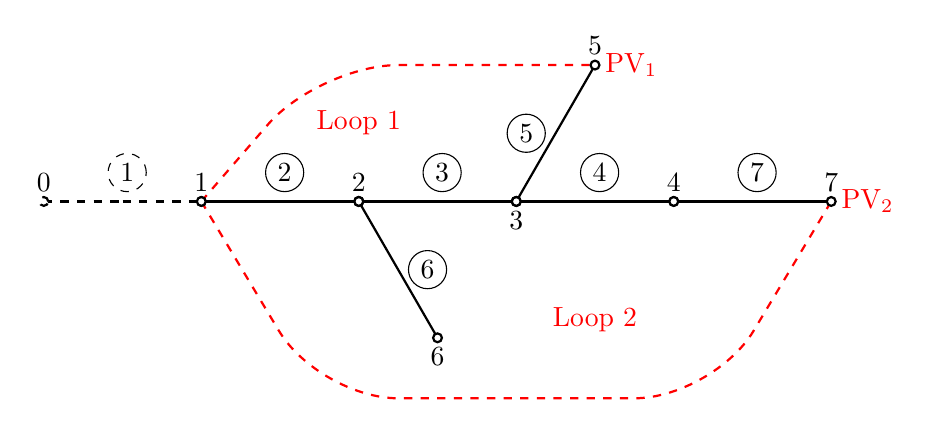
\begin{tikzpicture}[thick]
  \draw[dashed,red,rounded corners=10mm] (0,0) -- (1.5,1.732) -- (5,1.732);
  \draw[dashed,red,rounded corners=10mm] (0,0) -- (1.5,-2.5) -- (6.5,-2.5) -- (8,0);
  \centerarc[red,-stealth'](3,0.5)(135:45:1)
  \node[red] at (2,1) {Loop 1};
  \centerarc[red,-stealth'](5.5,-1)(270:360:1)
  \node[red] at (5,-1.5) {Loop 2};
  \node[above] at (-2,0) {0};
  \draw[dashed] (-2,0) to[short,o-o,l=\circled{1}] (0,0) node[above]{1};
  \draw (0,0) to[short,o-o,l=\circled{2}] (2,0) node[above]{2};
  \draw (2,0) to[short,o-o,l=\circled{3}] (4,0) node[below]{3};
  \draw (4,0) to[short,o-o,l=\circled{4}] (6,0) node[above]{4};
  \draw (6,0) to[short,o-o,l=\circled{7}] (8,0) node[above]{7};
  \node[red,right] at (8,0) {${\rm PV_2}$};
  \draw (2,0) to[short,o-o] ++(-60:2) node[below]{6};
  \node[right] at (2.5,-0.866) {\circled{6}};
  \draw (4,0) to[short,o-o] ++(60:2) node[above]{5};
  \node[red,right] at (5,1.732) {${\rm PV_1}$};
  \node[left] at (4.5,0.866) {\circled{5}};
  \end{tikzpicture}
  \caption{Oriented Ordering}
  \label{fig:ordering}
\end{figure}
As usual, the supply bus (slack bus) is given index 1, meaning that branch indices should go from 2 to $n_b$ which is the number of buses in the network. Introducing a fictitious branch with index 1 and zero impedance, given with dashed black line in \figurename~\ref{fig:ordering}, the number of branches $n_l$ becomes equal to the number of buses $n_b$.

For the example of \figurename~\ref{fig:ordering} vector~$F$ is the following
\begin{equation*}
  F = \trans{\left[\begin{array}{ccccccc}
    0 & 1 & 2 & 3 & 3 & 2 & 4
  \end{array}\right]},
\end{equation*}
and it offers an easy way to follow the path between any bus and bus~0. If we consider bus~4, the path to the slack bus consists of following branches: branch~4, since considered bus is their receiving bus; branch~3, since $f_4 = 3$; branch~2, since $f_3 = 2$; and branch~1, since $f_2 = 1$.

The representation of branch~$k$, connecting buses $i$ and $k$, is given in \figurename~\ref{fig:branch_rep}, where it is modeled with its serial impedance $z_s^k$. At both ends there are load demands $s_d^i$ and $s_d^k$, and shunt admittances $y_d^i$ and $y_d^k$ comprised of admittances due capacitance of all lines and shunt elements connected to buses $i$ and $k$
\begin{equation*}
  y_d^k = j \left( \sum b_{\rm lines}^k + \sum b_{\rm shunt}^k \right).
\end{equation*}

% \begin{figure}[htb]
%   \centering
%   \begin{tikzpicture}[thick]
%     \node[above] at (0,0) {$i$};
%     \draw (0,0) to[short,i=$s_f^k$] (1,0);
%     \draw (1,0) to[R,l=$z_s^k$] (3,0);
%     \draw (3,0) to[short,i=$s_t^k$] (4,0) node[above] {$k$};
%     \draw[-stealth'] (0,0) -- (0,-1) node[right] {$s_d^i$};
%     \draw (0,0) to[short,o-] (-1,-0.5) to[R,l=$y_d^i$,v=$v_i$] (-1,-2.5) node[rground] {};
%     \draw[-stealth'] (4,0) -- (4,-1) node[left] {$s_d^k$};
%     \draw (4,0) to[short,o-] (5,-0.5) to[R,l_=$y_d^k$,v^=$v_k$] (5,-2.5) node[rground] {};
%   \end{tikzpicture}
%   \caption{Branch Representation: branch $k$ between buses $i$ (sending) and $k$ (receiving) and load demand and shunt admittances at both buses}
%   \label{fig:branch_rep}
% \end{figure}

\begin{figure}[htb]
  \centering
  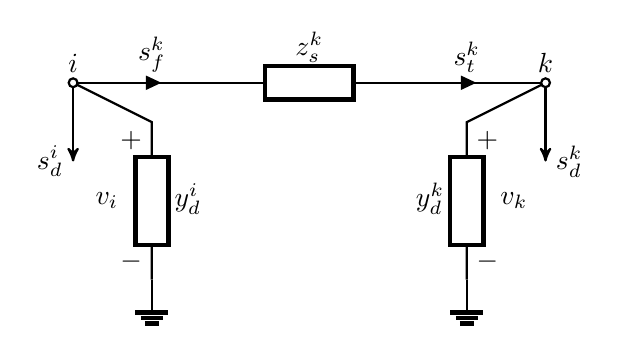
\begin{tikzpicture}[thick]
    \node[above] at (-1,0) {$i$};
    \draw (-1,0) to[short,i=$s_f^k$] (1,0);
    \draw (1,0) to[R,l=$z_s^k$] (3,0);
    \draw (3,0) to[short,i=$s_t^k$] (5,0) node[above] {$k$};
    \draw[-stealth'] (-1,0) -- (-1,-1) node[left] {$s_d^i$};
    \draw (-1,0) to[short,o-] (0,-0.5) to[R,l=$y_d^i$,v=$v_i$] (0,-2.5) node[ground] {};
    \draw[-stealth'] (5,0) -- (5,-1) node[right] {$s_d^k$};
    \draw (5,0) to[short,o-] (4,-0.5) to[R,l_=$y_d^k$,v^=$v_k$] (4,-2.5) node[ground] {};
  \end{tikzpicture}
  \caption{Branch Representation: branch $k$ between buses $i$ (sending) and $k$ (receiving) and load demand and shunt admittances at both buses}
  \label{fig:branch_rep}
\end{figure}

\subsubsection{Current Summation Method}
The voltage calculation procedure with the Current Summation Method is performed in 5 steps as follows \cite{shirmohammadi1988,luo1990}.

\begin{enumerate}
  
  \item Set all voltages to 1~p.u. (flat start). Set iteration count $\nu = 1$.
  
  \item Set branch current flow equal to the sum of current of the demand at receiving end ($s_d^k$) and the current drawn in the admittance ($y_d^k$) connected to bus~$k$
  \begin{equation}
  \label{eq:j_branch}
  j_b^k = \cc{\left(\frac{s_d^k}{v_k}\right)} + y_d^k \cdot v_k, \quad k = 1, 2, \ldots ,n_b.
  \end{equation}
  \label{step2i}
  
  \item \textit{Backward sweep}: Perform current summation, starting from the branch with the biggest index and heading towards the branch whose index is equal to 1. The current of branch $k$ is added to the current of the branch whose index is equal to $i = f_k$.
  \begin{equation}
  j_{b,\rm new}^i = j_b^i + j_b^k, \quad k = n_l, n_l - 1, \ldots ,2
  \label{eq:back_i}
  \end{equation}
  
  \item \textit{Forward sweep}: The receiving end bus voltages are calculated with known branch currents and sending bus voltages.
  \begin{equation}
  \label{eq:for_i}
  v_k = v_i - z_s^k \cdot j_b^k, \quad k = 2, 3, \ldots ,n_l
  \end{equation}
  
  \item Compare voltages in iteration $\nu$ with the corresponding ones from iteration ${\nu - 1}$. If the maximum difference in magnitude is less than the specified tolerance
  \begin{equation}
  \max_{i = 1 \ldots n_b} \left\lbrace \left| v_i^{\nu} - v_i^{\nu - 1} \right| \right\rbrace < \varepsilon
  \label{eq:tol_i}
  \end{equation}
  the procedure is finished. Otherwise go to step \ref{step2i}.
  
\end{enumerate}

\subsubsection{Power Summation Method}
The voltage calculation procedure with the Power Summation Method is performed in 5 steps as follows \cite{rajicic1994}.

\begin{enumerate}
  
  \item Set all voltages to 1~p.u. (flat start). Set iteration count $\nu = 1$.
  
  \item Set receiving end branch flow equal to the sum of the demand at receiving end ($s_d^k$) and the power drawn in the admittance ($y_d^k$) connected to bus~$k$
  \begin{equation}
  \label{eq:s_receiving}
  s_t^k = s_d^k + \frac{\cc{\left(y_d^k\right)}}{v_k^2}, \quad k = 1, 2, \ldots ,n_b.
  \end{equation}
  \label{step2pq}
  
  \item \textit{Backward sweep}: Calculate sending end branch power flows as a sum of receiving end branch power flows and branch losses via \eqref{eq:back_pq_1}. Perform power summation, starting from the branch with the biggest index and heading towards the branch whose index is equal to 1. The sending power of branch $k$ is added to the receiving power of the branch whose index is equal to $i = f_k$ as in \eqref{eq:back_pq_2}.
  \begin{align}
  s_f^k &= s_t^k + z_s^k \cdot \left|\frac{s_t^k}{v_k}\right|^2 & k = n_l, n_l - 1, \ldots ,2
  \label{eq:back_pq_1}
  \\
  s_{t,{\rm new}}^i &= s_t^i + s_f^k & k = n_l, n_l - 1, \ldots ,2
  \label{eq:back_pq_2}
  \end{align}
  
  \item \textit{Forward sweep}: The receiving end bus voltages are calculated with known sending powers and voltages.
  \begin{equation}
  \label{eq:for_pq}
  v_k = v_i - z_s^k \cdot \cc{\left(\frac{s_f^k}{v_i}\right)} \quad k = 2, 3, \ldots ,n_l
  \end{equation}
  
  \item Compare voltages in iteration $\nu$ with the corresponding ones from iteration ${\nu - 1}$, using \eqref{eq:tol_i}. If the maximum difference in magnitude is less than the specified tolerance the procedure is finished. Otherwise go to step \ref{step2pq}.
  
\end{enumerate}

\subsubsection{Admittance Summation Method}
For each node, besides the known admittance $y_d^k$, we define the admittance $y_e^k$ as the driving point admittance of the part of the network fed by node $k$, including shunt admittance $y_d^k$. We also define an equivalent current generator $j_e^k$ for the part of the network fed by node $k$. The current of this generator consists of all load currents fed by node $k$.
The process of calculation of bus voltages with the admittance summation method consists of the following 5 steps \cite{rajicic1998}.

\begin{enumerate}
  
  \item Set all voltages to 1~p.u. (flat start). Set iteration count $\nu = 1$. Set initial values
  \begin{equation}
    y_e^k = y_d^k, \quad k = 1, 2, \ldots ,n_b.
  \end{equation}

  \item For each node~$k$, calculate equivalent admittance $y_e^k$. Perform admittance summation, starting from the branch with the biggest index and heading towards the branch whose index is equal to 1. The driving point admittance of branch~$k$ is added to the driving point admittance of the branch whose index is equal to $i = f_k$ as in \eqref{eq:back_y_2a}.
  \begin{align}
  d_b^k &= \frac{1}{1 + z_s^k \cdot y_e^k} & k = n_l, n_l - 1, \ldots ,2
  \label{eq:back_y_1a}
  \\
  y_{e,{\rm new}}^i &= y_e^i + d_b^k \cdot y_e^k & k = n_l, n_l - 1, \ldots ,2
  \label{eq:back_y_2a}
  \end{align}
 
  \item \textit{Backward sweep}: For each node $k$ calculate equivalent current generator $j_e^k$, first set it equal to load current $j_d^k$ and perform current summation over equivalent admittances using factor $d_b^k$ as in \eqref{eq:back_y_1a}.
  \begin{align}
  j_e^k &= j_d^k = \cc{\left(\frac{s_d^k}{v_k}\right)} & k = n_l, n_l - 1, \ldots ,2
  \label{eq:back_y_1}
  \\
  j_{e,{\rm new}}^i &= j_e^i + d_b^k \cdot j_e^k & k = n_l, n_l - 1, \ldots ,2
  \label{eq:back_y_2}
  \end{align}
  \label{step3y}
  
  \item \textit{Forward sweep}: The receiving end bus voltages are calculated with known equivalent current generators and sending bus voltages.
  \begin{equation}
  \label{eq:for_y}
  v_k = d_b^k \cdot (v_i - z_s^k \cdot j_e^k) \quad k = 2, 3, \ldots ,n_l
  \end{equation}
  
  \item Compare voltages in iteration $\nu$ with the corresponding ones from iteration ${\nu - 1}$, using \eqref{eq:tol_i}. If the maximum difference in magnitude is less than the specified tolerance the procedure is finished. Otherwise go to step \ref{step3y}.
  
\end{enumerate}

\subsubsection{Handling PV Buses}
The methods explained in the previous three subsections are applicable to radial networks without loops and PV buses. These methods can be used to solve the power flow problem in weakly meshed networks if a compensation procedure based on Thevenin equivalent impedance matrix is added \cite{shirmohammadi1988,luo1990}. In \cite{rajicic1994} a voltage correction procedure is added to the process.

The list of branches is expanded by a set
of $n_{pv}$ fictitious links, corresponding to the PV nodes. Each of these links starts at the slack bus and ends at a corresponding PV bus, thus forming a loop in the network. A fictitious link going to bus~$k$ is represented by a voltage generator with a voltage magnitude equal to the specified voltage magnitude at bus~$k$. Its phase angle is equal to the calculated phase angle at bus~$k$.

A loop impedance matrix $Z_l$ is formed for the loops made by the fictitious links and it has the following properties
\begin{itemize}
\item Element $z_l^{mm}$ is equal to the sum of branch impedances of all branches related to loop $m$,
\item Element $z_l^{mk}$ is equal to the sum of branch impedances of mutual branches of loops $m$ and $k$.
\end{itemize}

As an illustration, in \figurename~\ref{fig:ordering} there a two PV generators at buses~5 and 7. The fictitious links and loops orientation are drawn in red. The Thevenin matrix for this case is
\begin{equation*}
Z_l = \left[\begin{array}{cc}
z_b^2 + z_b^3 + z_b^5 & z_b^2 + z_b^3 \\
z_b^2 + z_b^3 & z_b^2 + z_b^3 + z_b^4 + z_b^7
\end{array}
\right].
\end{equation*}

First column elements are equal to PV bus voltages when the current injection at bus~5 is 1~p.u. and $v_1 = 0$. Bus voltages can be calculated with the current summation method in a single iteration. By repeating the procedure for bus~7 one can calculate the elements of second column.

By breaking all links the network becomes radial \cite{luo1990} and the three backward/forward sweep methods are applicable. Since all links are fictitious, only the injected reactive power at their receiving bus $m$ is determined \cite{rajicic1994} by the following equation
\begin{equation}
\Delta q_{pv}^m = \Delta d_{pv}^m \frac{v_m^2}{\Re \left\{ v_m \right\} },
\end{equation}
which is practically an increment in reactive power injection of the corresponding PV generator for the current iteration.

The incremental changes of the imaginary part of PV generator current $\Delta d_{pv}^m$ can be obtained by solving the matrix equation
\begin{equation}
\Im \left\{ Z_l \right\}  \cdot \Delta D_{pv} = \Delta E_{pv},
\end{equation}
where
\begin{equation}
\Delta e_{pv}^m = \left( \frac{v_g^m}{ \left| v_m \right|  } - 1 \right) \cdot \Re \left\{ v_m \right\}, \quad m = 1, 2, \ldots , n_{pv}.
\end{equation}

In order to ensure $90^\circ$ phase difference between voltage and current at PV generators in \cite{Rajicic2001} it was suggested to calculate the real part of PV generator current as
\begin{equation}
\Delta c_{pv}^m = \Delta d_{pv}^m \frac{\Im \left\{ v_m \right\}}{\Re \left\{ v_m \right\}}.
\end{equation}
In such a way the PV generator will inject purely reactive power, as it is supposed to do. Its active power is added before as a negative load.

Before proceeding with the next iteration, the bus voltage corrections are calculated. In order to do that, the radial network is solved by applying incremental current changes $\Delta I_{pv} =  \Delta C_{pv} + j \Delta D_{pv}$ at the PV buses as excitations and setting $v_1 = 0$. After the backward/forward sweep is performed with the current summation method, the voltage corrections at all buses are known. They are added to the latest voltages in order to obtain the new bus voltages, which are used in the next iteration \cite{rajicic1994}.

\subsection{{\tt runpf}}
\label{sec:runpf}

In \matpower{}, a power flow is executed by calling \code{runpf} with a case struct or case file name as the first argument (\code{casedata}). In addition to printing output to the screen, which it does by default, \code{runpf} optionally returns the solution in a \results{} struct.
\begin{Code}
>> results = runpf(casedata);
\end{Code}
The \results{} struct is a superset of the input \matpower{} case struct \mpc{}, with some additional fields as well as additional columns in some of the existing data fields. The solution values are stored as shown in Table~\ref{tab:pfresults}.

\begin{table}[!ht]
%\renewcommand{\arraystretch}{1.2}
\centering
\begin{threeparttable}
\caption{Power Flow Results}
\label{tab:pfresults}
\footnotesize
\begin{tabular}{ll}
\toprule
name & description \\
\midrule
\code{results.success}	& success flag, 1 = succeeded, 0 = failed	\\
\code{results.et}	& computation time required for solution	\\
\code{results.iterations}	& number of iterations required for solution	\\
\code{results.order}	& see \code{ext2int} help for details on this field	\\
\code{results.bus(:, VM)}\tnote{\dag}	& bus voltage magnitudes	\\
\code{results.bus(:, VA)}	& bus voltage angles	\\
\code{results.gen(:, PG)}	& generator real power injections	\\
\code{results.gen(:, QG)}\tnote{\dag}	& generator reactive power injections	\\
\code{results.branch(:, PF)}	& real power injected into ``from'' end of branch	\\
\code{results.branch(:, PT)}	& real power injected into ``to'' end of branch	\\
\code{results.branch(:, QF)}\tnote{\dag}	& reactive power injected into ``from'' end of branch	\\
\code{results.branch(:, QT)}\tnote{\dag}	& reactive power injected into ``to'' end of branch	\\
\bottomrule
\end{tabular}
\begin{tablenotes}
 \scriptsize
 \item [\dag] {AC power flow only.}
\end{tablenotes}
\end{threeparttable}
\end{table}

\begin{table}[!ht]
%\renewcommand{\arraystretch}{1.2}
\centering
\begin{threeparttable}
\caption{Power Flow Options}
\label{tab:pfoptions}
\footnotesize
\begin{tabular}{lcp{0.62\textwidth}}
\toprule
name & default & description \\
\midrule
\code{model}	& \codeq{AC}	& AC vs. DC modeling for power flow and OPF formulation \\
&& \begin{tabular}{c @{ -- } l}
\codeq{AC} & use AC formulation and corresponding alg options \\
\codeq{DC} & use DC formulation and corresponding alg options \\
\end{tabular}	\\
\code{pf.alg}	& \codeq{NR}	& AC power flow algorithm: \\
&& \begin{tabular}{c @{ -- } p{0.5\textwidth}}
\codeq{NR} & Newtons's method (formulation depends on options \code{pf.current\_balance} and \code{pf.v\_cartesian})\tnote{\dag} \\
% \codeq{NR-SP} & Newtons's method (power mismatch, polar)\tnote{\dag} \\
% \codeq{NR-SC} & Newtons's method (power mismatch, cartesian)\tnote{\dag} \\
% \codeq{NR-SH} & Newtons's method (power mismatch, hybrid)\tnote{\dag} \\
% \codeq{NR-IP} & Newtons's method (current mismatch, polar)\tnote{\dag} \\
% \codeq{NR-IC} & Newtons's method (current mismatch, cartesian)\tnote{\dag} \\
% \codeq{NR-IH} & Newtons's method (current mismatch, hybrid)\tnote{\dag} \\
\codeq{FDXB} & Fast-Decoupled (XB version) \\
\codeq{FDBX} & Fast-Decouple (BX version) \\
\codeq{GS} & Gauss-Seidel \\
\codeq{PQSUM} & Power Summation (radial networks only) \\
\codeq{ISUM} & Current Summation (radial networks only) \\
\codeq{YSUM} & Admittance Summation (radial networks only) \\
\end{tabular}	\\
\code{pf.current\_balance}\tnote{\ddag}	& 0	& use current, as opposed to power, balance for AC PF, 0 or 1	\\
\code{pf.v\_cartesian}\tnote{\ddag}	& 0	& voltage representation	\\
&& \begin{tabular}{r @{ -- } l}
0 & bus voltage variables represented in polar coordinates \\
1 & bus voltage variables represented in cartesian coordinates \\
2 & hybrid, polar updates computed via modified cartesian Jacobian \\
\end{tabular}	\\
\code{pf.tol}	& $10^{-8}$	& termination tolerance on per unit P and Q dispatch	\\
\code{pf.nr.max\_it}	& 10	& maximum number of iterations for Newton's method	\\
\code{pf.nr.lin\_solver}	& \codeq{}	& linear solver option for \code{mplinsolve} for computing Newton update step \\
&& (see \code{mplinsolve} for complete list of all options)	\\
&& \begin{tabular}{c @{ -- } p{0.57\textwidth}}
\codeq{} & default to \codeq{\textbackslash} for small systems, \codeq{LU3} for larger ones \\
\codeq{\textbackslash} & built-in backslash operator \\
\codeq{LU} & explicit default LU decomposition and back substitution \\
\codeq{LU3} & 3 output arg form of \code{lu}, Gilbert-Peierls algorithm with approximate minimum degree (AMD) reordering \\
\codeq{LU4} & 4 output arg form of \code{lu}, UMFPACK solver (same as \codeq{LU}) \\
\codeq{LU5} & 5 output arg form of \code{lu}, UMFPACK solver w/row scaling \\
\end{tabular}	\\
\code{pf.fd.max\_it}	& 30	& maximum number of iterations for fast-decoupled method	\\
\code{pf.gs.max\_it}	& 1000	& maximum number of iterations for Gauss-Seidel method	\\
\code{pf.radial.max\_it}	& 20	& maximum number of iterations for radial power flow methods	\\
\code{pf.radial.vcorr}	& 0	& perform voltage correction procedure in distribution power flow	\\
&& \begin{tabular}{c @{ -- } l}
0 & do \emph{not} perform voltage correction \\
1 & perform voltage correction \\
\end{tabular}	\\
\code{pf.enforce\_q\_lims}	& 0	& enforce gen reactive power limits at expense of $|V_m|$	\\
&& \begin{tabular}{r @{ -- } l}
0 & do \emph{not} enforce limits \\
1 & enforce limits, simultaneous bus type conversion \\
2 & enforce limits, one-at-a-time bus type conversion \\
\end{tabular}	\\
\bottomrule
\end{tabular}
\begin{tablenotes}
 \scriptsize
%  \item [\dag] {Automatically sets/overrides \code{pf.current\_balance} and \code{pf.v\_cartesian} options with corresponding values.}
 \item [\dag] {The values \codeq{NR-SP}, \codeq{NR-SC}, \codeq{NR-SH}, \codeq{NR-IP}, \codeq{NR-IC}, \codeq{NR-IH} can also be used as shortcuts to simultaneously select Newton's method and set/override the \code{pf.current\_balance} and \code{pf.v\_cartesian} options with corresponding values, where \codeq{S} and \codeq{I} are for power and current balance, respectively, and \codeq{P}, \codeq{C} and \codeq{H} are for polar, cartesian and hybrid, respectively.}
 \item [\ddag] {Only relevant for Newton AC power flow solver.}
\end{tablenotes}
\end{threeparttable}
\end{table}

Additional optional input arguments can be used to set options (\code{mpopt}) and provide file names for saving the pretty printed output (\code{fname}) or the solved case data (\code{solvedcase}).
\begin{Code}
>> results = runpf(casedata, mpopt, fname, solvedcase);
\end{Code}
The options that control the power flow simulation are listed in Table~\ref{tab:pfoptions} and those controlling the output printed to the screen in Table~\ref{tab:pfoutputoptions}.

By default, \code{runpf} solves an AC power flow problem using a standard Newton's method solver. To run a DC power flow, the \code{model} option must be set to \codeq{DC}. For convenience, \matpower{} provides a function \code{rundcpf} which is simply a wrapper that sets the \code{model} option to \codeq{DC} before calling \code{runpf}.

\begin{table}[!ht]
%\renewcommand{\arraystretch}{1.2}
\centering
\begin{threeparttable}
\caption{Power Flow Output Options}
\label{tab:pfoutputoptions}
\footnotesize
\begin{tabular}{lcp{0.58\textwidth}}
\toprule
name & default & description \\
\midrule
\code{verbose}	& 1	& amount of progress info to be printed \\
&& \begin{tabular}{r @{ -- } l}
0 & print no progress info \\
1 & print a little progress info \\
2 & print a lot of progress info \\
3 & print all progress info \\
\end{tabular}	\\
\code{out.all}	& -1	& controls pretty-printing of results \\
&& \begin{tabular}{r @{ -- } l}
-1 & individual flags control what is printed \\
0 & do \emph{not} print anything\tnote{\dag} \\
1 & print everything\tnote{\dag} \\
\end{tabular}	\\
\code{out.sys\_sum}	& 1	& print system summary (0 or 1) \\
\code{out.area\_sum}	& 0	& print area summaries (0 or 1) \\
\code{out.bus}	& 1	& print bus detail, includes per bus gen info (0 or 1) \\
\code{out.branch}	& 1	& print branch detail (0 or 1) \\
\code{out.gen}	& 0	& print generator detail (0 or 1) \\
\code{out.force}	& 0	& print results even if success flag = 0 (0 or 1) \\
\code{out.suppress\_detail}	& -1	& suppress all output but system summary \\
&& \begin{tabular}{r @{ -- } l}
-1 & suppress details for large systems ($>$~500~buses) \\
0 & do \emph{not} suppress any output specified by other flags \\
1 & suppress all output except system summary section\tnote{\dag} \\
\end{tabular}	\\
\bottomrule
\end{tabular}
\begin{tablenotes}
 \scriptsize
 \item [\dag] {Overrides individual flags, but (in the case of \code{out.suppress\_detail}) not \code{out.all} = 1.}
\end{tablenotes}
\end{threeparttable}
\end{table}

Internally, the \code{runpf} function does a number of conversions to the problem data before calling the appropriate solver routine for the selected power flow algorithm. This external-to-internal format conversion is performed by the \code{ext2int} function, described in more detail in Section~\ref{sec:ext2int_callback}, and includes the elimination of out-of-service equipment and the consecutive renumbering of buses. All computations are done using this internal indexing. When the simulation has completed, the data is converted back to external format by \code{int2ext} before the results are printed and returned.

\subsection{Linear Shift Factors}
\label{sec:lsf}

The DC power flow model can also be used to compute the sensitivities of branch flows to changes in nodal real power injections, sometimes called injection shift factors (ISF) or generation shift factors~\cite{wood1996}. These $n_l \times n_b$ sensitivity matrices, also called power transfer distribution factors or PTDFs, carry an implicit assumption about the slack distribution. If $H$ is used to denote a PTDF matrix, then the element in row~$i$ and column~$j$, $h_{ij}$, represents the change in the real power flow in branch~$i$ given a unit increase in the power injected at bus~$j$, \emph{with the assumption} that the additional unit of power is extracted according to some specified slack distribution:
\begin{equation}
\Delta P_f = H \Delta P_\mathrm{bus}.
\end{equation}

This slack distribution can be expressed as an $n_b \times 1$ vector $w$ of non-negative weights whose elements sum to 1. Each element specifies the proportion of the slack taken up at each bus. For the special case of a single slack bus~$k$, $w$ is equal to the vector $e_k$. The corresponding PTDF matrix $H_k$ can be constructed by first creating the $n_l \times (n_b-1)$ matrix
\begin{equation}
\widetilde{H}_k = \widetilde{B}_f \cdot B_{dc}^{-1}
\end{equation}
then inserting a column of zeros at column~$k$. Here $\widetilde B_f$ and $B_{dc}$ are obtained from $B_f$ and $B_\mathrm{bus}$, respectively, by eliminating their reference bus columns and, in the case of $B_{dc}$, removing row~$k$ corresponding to the slack bus.

The PTDF matrix $H_w$, corresponding to a general slack distribution $w$, can be obtained from any other PTDF, such as $H_k$, by subtracting $H_k \cdot w$ from each column, equivalent to the following simple matrix multiplication:
\begin{equation}
H_w = H_k (I - w \cdot \trans{1}).
\end{equation}

These same linear shift factors may also be used to compute sensitivities of branch flows to branch outages, known as line outage distribution factors or LODFs~\cite{guler2007}. Given a PTDF matrix $H_w$, the corresponding $n_l \times n_l$ LODF matrix $L$ can be constructed as follows, where $l_{ij}$ is the element in row~$i$ and column~$j$, representing the change in flow in branch~$i$ (as a fraction of the initial flow in branch~$j$) for an outage of branch~$j$.

First, let $H$ represent the matrix of sensitivities of branch flows to branch endpoint injections, found by multplying the PTDF matrix by the node-branch incidence matrix:
\begin{equation}
H = H_w \trans{(C_f - C_t)}.
\end{equation}
Here the individual elements $h_{ij}$ represent the sensitivity of flow in branch~$i$ with respect to injections at branch~$j$ endpoints, corresponding to a simulated increase in flow in branch~$j$. Then $l_{ij}$ can be expressed as
\begin{equation}
l_{ij} = \left\{\begin{array}{cc}
\displaystyle\frac{h_{ij}}{1 - h_{jj}} & i \neq j \\
-1 & i = j.
\end{array}
\right.
\end{equation}

\matpower{} includes functions for computing both the DC PTDF matrix and the corresponding LODF matrix for either a single slack bus~$k$ or a general slack distribution vector $w$. See the help for \code{makePTDF} and \code{makeLODF} and Sections~\ref{sec:makePTDF} and \ref{sec:makeLODF}, respectively, for details.


%%------------------------------------------
\clearpage
\section{Continuation Power Flow}

Continuation methods or branch tracing methods are used to trace a curve given an initial point on the curve. These are also called predictor-corrector methods since they involve the prediction of the next solution point and correcting the prediction to get the next point on the curve.

Consider a system of $n$ nonlinear equations $g(x) = 0, x \in \mathbb{R}^n$. By adding a continuation parameter $\lambda$ and one more equation to the system, $x$ can be traced by varying $\lambda$. The resulting system $f(x,\lambda)=0$ has $n + 1$ dimensions. The additional equation is a parameterized equation which identifies the location of the current solution with respect to the previous or next solution.

The continuation process can be diagrammatically shown by \eqref{eq:cpf1}.
\begin{equation}
\left(x^j,\lambda^j\right) \xrightarrow{Predictor} (\hat{x}^{j+1},\hat{\lambda}^{j+1}) \xrightarrow{Corrector} \left({x}^{j+1},{\lambda}^{j+1}\right)
\label{eq:cpf1}
\end{equation}
where, $\left(x^j,\lambda^j\right)$ represents the current solution at step~$j$, $(\hat{x}^{j+1},\hat{\lambda}^{j+1})$ is the predicted solution for the next step, and $({x}^{j+1},{\lambda}^{j+1})$ is the next solution on the curve.

Continuation methods are employed in power systems to determine steady state stability limits \cite{ajjarapu1992} in what is called a continuation power flow\footnote{Thanks to Shrirang Abhyankar, Rui Bo, and Alexander Flueck for contributions to \matpower{}'s continuation power flow feature.}. The limit is determined from a nose curve where the nose represents the maximum power transfer that the system can handle given a power transfer schedule. To determine the steady state loading limit, the basic power flow equations
\begin{equation}  g(x) = \left[ \begin{array}{c}
P(x) - P^{inj} \\
Q(x) - Q^{inj}  \end{array} \right] = 0,
\label{eq:pf}
\end{equation}
are restructured as 
\begin{equation}
f(x,\lambda) = g(x) - \lambda{b} = 0
\label{eq:fxlam}
\end{equation}
where $x \equiv \left(\Theta, V_m\right)$ and $b$ is a vector of power transfer given by
\begin{equation}  b = \left[ \begin{array}{c}
P_{target}^{inj} - P_{base}^{inj} \\
Q_{target}^{inj} - Q_{base}^{inj}  \end{array} \right].
\label{eq:Sxfr}
\end{equation}
The effects of the variation of loading or generation can be investigated using the continuation method by composing the $b$ vector appropriately.

\subsection{Parameterization}

The values of $(x, \lambda)$ along the solution curve can parameterized in a number of ways \cite{chiang1995, li2008}. Parameterization is a mathematical way of identifying each solution so that the \emph{next} solution or \emph{previous} solution can be quantified. \matpower{} includes three parameterization scheme options to quantify this relationship, detailed below, where $\sigma$ is the continuation step size parameter.

\begin{itemize}

\item{\bf Natural parameterization} simply uses $\lambda$ directly as the parameter, so the new $\lambda$ is simply the previous value plus the step size.
\begin{equation}
p^j(x,\lambda) = \lambda - \lambda^j - \sigma^j = 0
\label{eq:natural_parm}
\end{equation}

\item {\bf Arc length parameterization} results in the following relationship, where the step size is equal to the 2-norm of the distance from one solution to the next.
\begin{equation}
p^j(x,\lambda) = \sum\limits_i(x_i - x_i^j)^2 + (\lambda - \lambda^j)^2 - (\sigma^j)^2 = 0
\label{eq:arc_parm}
\end{equation}
\item {\bf Pseudo arc length parameterization} \cite{mori2002} is \matpower{}'s default parameterization scheme, where the next point $(x,\lambda)$ on the solution curve is constrained to lie in the hyperplane running through the predicted solution $(\hat{x}^{j+1}, \hat{\lambda}^{j+1})$ orthogonal to the tangent line from the previous corrected solution $(x^j,\lambda^j)$. This relationship can be quantified by the function
\begin{equation}
p^j(x,\lambda) = \trans{ \left(\left[\begin{array}{c}x \\ \lambda\end{array}\right] - \left[\begin{array}{c}x^{j} \\ \lambda^j\end{array}\right]\right) } \bar{z}^j -\sigma^j = 0,
\label{eq:psuedo_arc_parm}
\end{equation}
where $\bar{z}^j$ is the normalized tangent vector at $(x^j, \lambda^j)$ and $\sigma^j$ is the continuation step size parameter.

\end{itemize}

\subsection{Predictor}
The predictor is used to produce an estimate for the next solution. The better the prediction, the faster is the convergence to the solution point. \matpower{} uses a tangent predictor for estimating the curve to the next solution. The tangent vector $z^j = \trans{\left[ \begin{array}{cc}dx & d\lambda \end{array} \right]_j}$ at the current solution $(x^j,\lambda^j)$ is found by solving the linear system
\begin{equation}
\left[ \begin{array}{cc}
  f_x & f_\lambda \\
  p^{j-1}_x & p^{j-1}_\lambda
\end{array} \right] z^j =
\left[ \begin{array}{c}
  0 \\
  1  \end{array} \right].
\label{eq:tangent_predictor}
\end{equation}
The matrix on the left-hand side is simply the standard power flow Jacobian with an additional column and row added. The extra column $f_\lambda$ is simply the negative of the power transfer vector $b$ and the extra row, required to make the system non-singular and define the magnitude of $z^j$, is the derivative of the the parameterization function at the previous solution point $p^{j-1}$.

The resulting tangent vector is then normalized
\begin{equation}
\bar{z}^j = \frac{z^j}{|| z^j ||_2}
\end{equation}
and used to compute the predicted approximation $(\hat{x}^{j+1},\hat{\lambda}^{j+1})$ to the next solution $\left({x}^{j+1},{\lambda}^{j+1}\right)$ using
\begin{equation}
\left[\begin{array}{c}\hat{x}^{j+1} \\ \hat{\lambda}^{j+1}\end{array}\right] = 
\left[\begin{array}{c}x^j \\ \lambda^j \end{array}\right] + \sigma^j \bar{z}^j,
\end{equation}
where $\sigma^j$ is the continuation step size.

\subsection{Corrector}
The corrector stage finds the next solution $\left(x^{j+1},\lambda^{j+1}\right)$ by correcting the approximation estimated by the predictor $(\hat{x}^{j+1},\hat{\lambda}^{j+1})$. Newton's method is used to find the next solution by solving the $n+1$ dimensional system in \eqref{eq:corrector}, where one of \eqref{eq:natural_parm}--\eqref{eq:psuedo_arc_parm} has been added as an additional constraint to the parameterized power flow equations of \eqref{eq:fxlam}.
\begin{equation} \left[\begin{array}{c}
 f(x,\lambda) \\
 p^j(x,\lambda)
 \end{array} \right]= 0
 \label{eq:corrector}
\end{equation}

\subsection{Step Length Control}
Step length control is a key element affecting the computational efficiency of a continuation method. It affects the continuation method with two issues: (1) speed -- how fast the corrector converges to a specified accuracy, and (2) robustness -- whether the corrector converges to a true solution given a predicted point. \matpower{}'s continuation power flow can optionally use adaptive steps, where the step size $\sigma$ is adjusted by a scaling factor $\alpha$ within the limits specified.
\begin{equation}
 \sigma^{j+1} = \alpha^j \sigma^j, \qquad \sigma_\mathrm{min} \le \sigma^{j+1} \le \sigma_\mathrm{max}
 \label{eq:cpf_step_adapt1}
\end{equation}
This scaling factor $\alpha^j$ for step~$j$ is limited to a maximum of 2 and is calculated from an error estimation between the predicted and corrected solutions $\gamma^j$ as follows,
\begin{equation}
 \alpha^j = 1 + \beta_\mathrm{cpf} \left(\dfrac{\epsilon_\mathrm{cpf}}{\gamma^j} - 1\right), \qquad \alpha^j \le 2,
 \label{eq:cpf_step_adapt2}
\end{equation}
where $\beta_\mathrm{cpf}$ is a damping factor, $\epsilon_\mathrm{cpf}$ is a specified tolerance, and $\gamma^j$ is given by
\begin{equation}
 \gamma^j = \left\Vert\left(x^{j+1},\lambda^{j+1}\right)-\left(\hat{x}^{j+1},\hat{\lambda}^{j+1}\right)\right\Vert_\infty.
 \label{eq:cpf_step_adapt3}
\end{equation}

\subsection{Event Detection and Location}
A continuation power flow \emph{event} is triggered when the value of one of the elements of an event function changes sign from one continuation step to the next. The event occurs at the point where the corresponding value of the event function passes through zero. \matpower{} provides event functions to detect the location at which the continuation power flow reaches the following:
\begin{itemize}
    \item a specified target $\lambda$ value
    \item the nose point
    \item the end of a full trace
    \item a generator reactive power limit
    \item a generator active power limit
    \item a bus voltage magnitude limit
    \item a branch flow limit
\end{itemize}

Each event function is registered with an event name, a flag indicating whether or not the location of the event should be pinpointed, and if so, to within what tolerance. For events that are to be located, when an event interval is detected, that is, when an element of the event function value changes sign, \matpower{} adjusts the continuation step size via a False Position or Regula Falsi method until it locates the point of the zero-crossing to within the specified tolerance.

The detection of an event zero, or even an event interval, can be used to trigger further actions. The CPF callback function capability was extended in \matpower{} 6.x to include the ability to handle events by including information about any event intervals or zeros detected. For example, \matpower{} includes a callback that fixes the reactive output of a generator and converts its bus from PV to PQ when the corresponding event function indicates that its reactive power limit has been reached. Another responds to the detection of the nose point by signaling the termination of the continuation. In fact, continuation power flow termination for nose point, target lambda or full trace modes are all based on CPF callback functions in conjunction with event detection.

While \matpower{} does include a mechanism for supplying user defined callback functions, it does not yet have a corresponding mechanism for user specified event functions.

\subsection{\tt{runcpf}}

In \matpower{}, a continuation power flow is executed by calling \code{runcpf} with two \matpower{} cases (case structs or case file names) as the first two arguments, \code{basecasedata} and \code{targetcasedata}, respectively. The first contains the base loading/generation profile while the second contains the target loading/generation profile. In addition to printing output to the screen, which it does by default, \code{runcpf} optionally returns the solution in a results struct.
\begin{Code}
>> results = runcpf(basecasedata, targetcasedata);
\end{Code}

Additional optional input arguments can be used to set options (\code{mpopt}) and provide file names for saving the pretty printed output (\code{fname}) or the solved case data (\code{solvedcase}).

\begin{Code}
>> results = runcpf(basecasedata, targetcasedata, mpopt, fname, solvedcase);
\end{Code}

The \results{} struct is a superset of the input \matpower{} case struct \mpc{}, with some additional fields as well as additional columns in some of the existing data fields. In addition to the solution values included in the \results{} for a simple power flow, shown in Table~\ref{tab:pfresults} in Section~\ref{sec:runpf}, the following additional continuation power flow solution values are stored in the \code{cpf} field as shown in Table~\ref{tab:cpfresults}.

\begin{table}[!ht]
%\renewcommand{\arraystretch}{1.2}
\centering
\begin{threeparttable}
\caption{Continuation Power Flow Results}
\label{tab:cpfresults}
\footnotesize
\begin{tabular}{lp{0.75\textwidth}}
\toprule
name & description \\
\midrule
\code{results.cpf}	& CPF output struct whose content depends on any user callback functions, where default contains fields: \\
\code{~~~~done\_msg}	& string with message describing cause of continuation termination \\
\code{~~~~events(eidx)} & a structure array of size $n_e$, where $n_e$ is the number of events located, with fields: \\
\code{~~~~~~k}	& continuation step number at which event was located \\
\code{~~~~~~name}	& name of event \\
\code{~~~~~~idx}	& index(es) of critical elements in corresponding event function, e.g. index of generator reaching VAr limit \\
\code{~~~~~~msg}	& descriptive text detailing the event \\
\code{~~~~iterations}	& $n_\mathrm{steps}$, number of continuation steps performed \\
\code{~~~~lam}	& $1 \times n$ vector of $\lambda$ values from correction steps\tnote{\dag} \\
\code{~~~~lam\_hat}	& $1 \times n$ vector of $\lambda$ values from prediction steps\tnote{\dag} \\
\code{~~~~max\_lam}	& maximum value of $\lambda$ found in \code{results.cpf.lam} \\
\code{~~~~steps}	& $1 \times n$ vector of step sizes for each continuation step performed\tnote{\dag} \\
\code{~~~~V}	& $n_b \times n$ matrix of complex bus voltages from correction steps\tnote{\dag} \\
\code{~~~~V\_hat}	& $n_b \times n$ matrix of complex bus voltages from prediction steps\tnote{\dag} \\
\bottomrule
\end{tabular}
\begin{tablenotes}
 \scriptsize
 \item [\dag] {$n$ is one more than the number of continuation steps, i.e. $n_\mathrm{steps}+1$, so the first element corresponds to the starting point.}
\end{tablenotes}
\end{threeparttable}
\end{table}

The options that control the continuation power flow simulation are listed in Table \ref{tab:cpfoptions}. All the power flow options for Newton's method (tolerance, maximum iterations) and for controlling the output on the screen (see Tables~\ref{tab:pfoptions} and \ref{tab:pfoutputoptions}) are also available with the continuation power flow.
\begin{table}[!ht]
\centering
\begin{threeparttable}
\caption{Continuation Power Flow Options}
\label{tab:cpfoptions}
\footnotesize
\begin{tabular}{lcp{0.57\textwidth}}
\toprule
name & default & description \\
\midrule
 \code{cpf.parameterization} & 3 & choice of parameterization \\
    & & ~1 --- natural \\
    & & ~2 --- arc length \\
    & & ~3 --- pseudo arc length \\
 \code{cpf.stop\_at} & \codeq{NOSE} & determines stopping criterion \\
    & & ~\codeq{NOSE} --- stop when nose point is reached \\
    & & ~\codeq{FULL} --- trace full nose curve \\
    & & ~$\lambda_\mathrm{stop}$ --- stop upon reaching target $\lambda$ value $\lambda_\mathrm{stop}$ \\
 \code{cpf.enforce\_p\_lims}	& 0	& enforce gen active power limits	\\
   & & ~0 --- do \emph{not} enforce limits \\
   & & ~1 --- enforce limits \\
 \code{cpf.enforce\_q\_lims}	& 0	& enforce gen reactive power limits at expense of $V_m$	\\
   & & ~0 --- do \emph{not} enforce limits \\
   & & ~1 --- enforce limits \\
 \code{cpf.enforce\_v\_lims}	& 0	& enforce bus voltage magnitude limits	\\
   & & ~0 --- do \emph{not} enforce limits \\
   & & ~1 --- enforce limits \\
 \code{cpf.enforce\_flow\_lims}	& 0	& enforce branch MVA flow limits	\\
   & & ~0 --- do \emph{not} enforce limits \\
   & & ~1 --- enforce limits \\
 \code{cpf.step} & 0.05 & default value for continuation power flow step size $\sigma$ \\
 \code{cpf.step\_min} & $10^{-4}$ & minimum allowed step size, $\sigma_\mathrm{min}$ \\
 \code{cpf.step\_max} & 0.2 & maximum allowed step size, $\sigma_\mathrm{max}$ \\
 \code{cpf.adapt\_step} & 0 & toggle adaptive step size feature \\
    & & ~0 --- adaptive step size disabled \\
    & & ~1 --- adaptive step size enabled \\
 \code{cpf.adapt\_step\_damping} & 0.7 & damping factor $\beta_\mathrm{cpf}$ from \eqref{eq:cpf_step_adapt2} for adaptive step sizing \\
 \code{cpf.adapt\_step\_tol} &  $10^{-3}$ & tolerance $\epsilon_\mathrm{cpf}$ from \eqref{eq:cpf_step_adapt2} for adaptive step sizing \\
 \code{cpf.target\_lam\_tol} &  $10^{-5}$ & tolerance for target lambda detection \\
 \code{cpf.nose\_tol} &  $10^{-5}$ & tolerance for nose point detection (p.u.) \\
 \code{cpf.p\_lims\_tol} &  $10^{-2}$ & tolerance for generator active power limit detection (MW) \\
 \code{cpf.q\_lims\_tol} &  $10^{-2}$ & tolerance for generator reactive power limit detection (MVAr) \\
 \code{cpf.v\_lims\_tol} &  $10^{-4}$ & tolerance for bus voltage magnitude limit detection (p.u) \\
 \code{cpf.flow\_lims\_tol} &  0.01 & tolerance for branch flow limit detection (MVA) \\
 \code{cpf.plot.level} & 0 & control plotting of nose curve \\
    & & ~0 --- do not plot nose curve \\
    & & ~1 --- plot when completed \\
    & & ~2 --- plot incrementally at each iteration \\
    & & ~3 --- same as 2, with \code{pause} at each iteration \\
 \code{cpf.plot.bus} & \emph{empty} & index of bus whose voltage is to be plotted \\
 \code{cpf.user\_callback} & \emph{empty} & string or cell array of strings with names of user callback functions\tnote{\dag} \\
\bottomrule
\end{tabular}
\begin{tablenotes}
 \scriptsize
 \item [\dag] {See \code{help cpf\_default\_callback} for details.}
\end{tablenotes}
\end{threeparttable}
\end{table}

\clearpage
\subsubsection{CPF Callback Functions}

\matpower{}'s continuation power flow provides a callback mechanism to give the user access to the iteration process for executing custom code at each iteration, for example, to implement custom incremental plotting of a PV nose curve or to handle a detected event. This callback mechanism is used internally to handle default plotting functionality as well as to handle the standard CPF events. The \code{cpf\_default\_callback} function, for example, is used to collect the $\lambda$ and $V$ results from each predictor and corrector iteration and optionally plot the PV nose curve.

The prototype for a CPF callback function is
\begin{Code}
function [nx, cx, done, rollback, evnts, cb_data, results] = ...
    cpf_user_callback(k, nx, cx, px, done, rollback, evnts, ...
                            cb_data, cb_args, results)
\end{Code}
and the input and output arguments are described in Tables~\ref{tab:cpf_callback_in} through \ref{tab:cpf_state} and in the help for \code{cpf\_default\_callback}. Each registered CPF callback function is called in three different contexts, distinguished by the value of the first argument \code{k} as follows:
\begin{enumerate}
\item{\em initial} -- called with \code{k} = 0, without \results{} input/output arguments, after base power flow, before first CPF step.
\item{\em iterations} -- called with \code{k} $> 0$, without \results{} input/output arguments, at each iteration, after predictor-corrector step
\item{\em final} -- called with \code{k} $< 0$, with \results{} input/output arguments, after exiting predictor-corrector loop, inputs identical to last iteration call, except \code{k} negated
\end{enumerate}

\begin{table}[!ht]
\centering
\begin{threeparttable}
\caption{Continuation Power Flow Callback Input Arguments}
\label{tab:cpf_callback_in}
\footnotesize
\begin{tabular}{p{0.18\textwidth}p{0.75\textwidth}}
\toprule
name & description \\
\midrule
\code{k}	&  continuation step iteration count \\
\code{nx}	&  next CPF state\tnote{*}, corresponding to proposed next step \\
\code{cx}	&  current CPF state\tnote{*}, corresponding to most recent successful step \\
\code{px}	&  previous CPF state\tnote{*}, corresponding to last successful step prior to \code{cx} \\
\code{done}	&  struct, with flag to indicate CPF termination and reason, with fields: \\
\code{~~.flag}	& termination flag, 1 $\rightarrow$ terminate, 0 $\rightarrow$ continue \\
\code{~~.msg}	& string containing reason for termination \\
\code{rollback}	&  scalar flag to indicate that the current step should be rolled back and retried with a different step size, etc. \\
\code{evnts}	&  struct array listing any events detected for this step\tnote{\ddag} \\
\code{cb\_data}	& struct containing static data\tnote{\S}~, with the following fields (all based on internal indexing): \\
\code{~~.mpc\_base}	& \matpower{} case struct of base case \\
\code{~~.mpc\_target}	& \matpower{} case struct of target case \\
\code{~~.Sbusb}	& handle of function returning $n_b \times 1$ vector of complex base case bus injections in p.u. and derivatives w.r.t. $|V|$ \\
\code{~~.Sbust}	& handle of function returning $n_b \times 1$ vector of complex target case bus injections in p.u. and derivatives w.r.t. $|V|$ \\
\code{~~.Ybus}	& bus admittance matrix \\
\code{~~.Yf}	& branch admittance matrix, ``from'' end of branches \\
\code{~~.Yt}	& branch admittance matrix, ``to'' end of branches \\
\code{~~.pv}	& list of indices of PV buses \\
\code{~~.pq}	& list of indices of PQ buses \\
\code{~~.ref}	& list of indices of reference buses \\
\code{~~.idx\_pmax}	& vector of gen indices of gens at PMAX \\
\code{~~.mpopt}	& \matpower{} options struct \\
\code{cb\_args}	&  arbitrary data structure containing user-provided callback arguments \\
\code{results}	& initial value of output struct to be assigned to \code{cpf} field of results struct returned by \code{runcpf} \\
\bottomrule
\end{tabular}
\begin{tablenotes}
 \scriptsize
 \item [*] {See Table~\ref{tab:cpf_state} for details of the CPF state.}
 \item [\ddag] {See \code{cpf\_detect\_events} for details of the \code{evnts} field.}
 \item [\S] {Please note that any callback that modifies the underlying problem is responsible to update the contents of \code{cb\_data} accordingly. E.g. converting a bus from PV to PQ requires updates to \code{mpc\_base}, \code{mpc\_target}, \code{Sbusb}, \code{Sbust}, \code{pv}, \code{pq}, and possibly \code{ref}. So, \code{cb\_data} should only be thought of as static for a fixed base and target case pair.}
\end{tablenotes}
\end{threeparttable}
\end{table}

\begin{table}[!ht]
\centering
\begin{threeparttable}
\caption{Continuation Power Flow Callback Output Arguments}
\label{tab:cpf_callback_out}
\footnotesize
\begin{tabular}{p{0.18\textwidth}p{0.75\textwidth}}
\toprule
name & description \\
\midrule
\multicolumn{2}{c}{\emph{All are updated versions of the corresponding input arguments, see Table~\ref{tab:cpf_callback_in} for more details.}} \\
\code{nx}	&  next CPF state\tnote{*}, user state (\code{cb} field) should be updated here if \code{rollback} is false \\
\code{cx}	&  current CPF state\tnote{*}, may contain updated \code{this\_step} or \code{this\_parm} values to be used if \code{rollback} is true \\
\code{done}	&  callback may have requested termination and set the \code{msg} field \\
\code{rollback}	&  callback can request a rollback step, even if it was not indicated by an event function\tnote{\dag} \\
\code{evnts}	&  \code{msg} field for a given event may be updated\tnote{\ddag} \\
\code{cb\_data}	& this data should only be modified if the underlying problem has been changed (e.g. generator limit reached), in which case it should always be followed by a step of zero length, i.e. set \code{nx.this\_step} to 0\tnote{\S} \\
\code{results}	& updated version of \results{} input argument to be assigned to \code{cpf} field of results struct returned by \code{runcpf} \\
\bottomrule
\end{tabular}
\begin{tablenotes}
 \scriptsize
 \item [*] {See Table~\ref{tab:cpf_state} for details of the CPF state.}
 \item [\dag] {In this case, the callback should also modify the step size or parameterization to be used for the re-try, by setting the \code{this\_step} or \code{this\_parm} fields in \code{cx}.}
 \item [\ddag] {See \code{cpf\_detect\_events} for details of the \code{evnts} field.}
 \item [\S] {It is the job of any callback modifying \code{cb\_data} to ensure that all data in \code{cb\_data} is kept consistent.}
\end{tablenotes}
\end{threeparttable}
\end{table}

\begin{table}[!ht]
\centering
\begin{threeparttable}
\caption{Continuation Power Flow State}
\label{tab:cpf_state}
\footnotesize
\begin{tabular}{p{0.18\textwidth}p{0.75\textwidth}}
\toprule
name & description \\
\midrule
\code{lam\_hat}	& value of $\lambda$ after predictor step \\
\code{V\_hat}	& vector of complex bus voltages after predictor step \\
\code{lam}	& value of $\lambda$ after corrector step \\
\code{V}	& vector of complex bus voltages after corrector step \\
\code{z}	& normalized tangent predictor, $\bar{z}$ \\
\code{default\_step}	& default step size \\
\code{default\_parm}	& default parameterization\tnote{*} \\
\code{this\_step}	& step size for this step only \\
\code{this\_parm}	& parameterization\tnote{*}~ for this step only \\
\code{step}	& current step size \\
\code{parm}	& current parameterization\tnote{*} \\
\code{events}	& event log \\
\code{cb}	& user state for callbacks\tnote{\dag}~, a user-defined struct containing any information a callback function would like to pass from one invokation to the next \\
\code{ef}	& cell array of event function values \\
\bottomrule
\end{tabular}
\begin{tablenotes}
 \scriptsize
 \item [*] {Corresponding to the \code{cpf.parameterization} option in  Table~\ref{tab:cpfoptions}.}
 \item [\dag] {Replaces \code{cb\_state} from \matpower{} 5.}
\end{tablenotes}
\end{threeparttable}
\end{table}

The user can define their own callback functions which take the same form and are called in the same contexts as \code{cpf\_default\_callback}. User callback functions are specified via the \matpower{} option \code{cpf.user\_callback}. This option can be a string containing the name of the callback function, or a struct with the following fields, where all but the first are optional:
\begin{itemize}
\item \code{fcn}       - string with name of callback function
\item \code{priority}  - numerical value specifying callback priority,\footnote{See \code{cpf\_register\_callback} for details.} default = 20
\item \code{args}      - arbitrary value (any type) passed to the callback
            as \code{cb\_args} each time it is invoked
\end{itemize}
Multiple user callbacks can be registered by assigning a cell array of such strings and/or structs to the \code{cpf.user\_callback} option.

\clearpage
\subsubsection{CPF Example}

The following is an example of running a continuation power flow using a version of the 9-bus system, looking at increasing all loads by a factor of 2.5. This example plots the nose curve shown in \figurename~\ref{fig:nose_curve}.
\begin{figure}[!htp]
  \centering
  \includegraphics[width=0.8\textwidth]{./figures/nose-curve}
  \caption{Nose Curve of Voltage Magnitude at Bus 9}
  \label{fig:nose_curve}
\end{figure}

\begin{Code}
define_constants;
mpopt = mpoption('out.all', 0, 'verbose', 2);
mpopt = mpoption(mpopt, 'cpf.stop_at', 'FULL', 'cpf.step', 0.2);
mpopt = mpoption(mpopt, 'cpf.plot.level', 2);
mpcb = loadcase('t_case9_pfv2');                    % load base case
mpct = mpcb;                                        % set up target case with
mpct.gen(:, [PG QG]) = mpcb.gen(:, [PG QG]) * 2.5;  % increased generation
mpct.bus(:, [PD QD]) = mpcb.bus(:, [PD QD]) * 2.5;  % and increased load
results = runcpf(mpcb, mpct, mpopt);
\end{Code}
This should result in something like the following output to the screen.
\begin{Code}
MATPOWER Version 7.0, 20-Jun-2019 -- AC Continuation Power Flow
step   0  :                      lambda =  0.000,  4 Newton steps
step   1  : stepsize = 0.2       lambda =  0.181   2 corrector Newton steps
step   2  : stepsize = 0.2       lambda =  0.359   2 corrector Newton steps
step   3  : stepsize = 0.2       lambda =  0.530   2 corrector Newton steps
step   4  : stepsize = 0.2       lambda =  0.693   3 corrector Newton steps
step   5  : stepsize = 0.2       lambda =  0.839   3 corrector Newton steps
step   6  : stepsize = 0.2       lambda =  0.952   3 corrector Newton steps
step   7  : stepsize = 0.2       lambda =  0.988   3 corrector Newton steps
step   8  : stepsize = 0.2       lambda =  0.899   3 corrector Newton steps
step   9  : stepsize = 0.2       lambda =  0.776   3 corrector Newton steps
step  10  : stepsize = 0.2       lambda =  0.654   3 corrector Newton steps
step  11  : stepsize = 0.2       lambda =  0.533   2 corrector Newton steps
step  12  : stepsize = 0.2       lambda =  0.413   2 corrector Newton steps
step  13  : stepsize = 0.2       lambda =  0.294   2 corrector Newton steps
step  14  : stepsize = 0.2       lambda =  0.176   2 corrector Newton steps
step  15  : stepsize = 0.2       lambda =  0.060   2 corrector Newton steps
step  16a : stepsize = 0.2       lambda = -0.054   2 corrector Newton steps ^ ROLLBACK
step  16  : stepsize = 0.0604    lambda =  0.000   3 corrector Newton steps
CPF TERMINATION: Traced full continuation curve in 16 continuation steps
\end{Code}
The results of the continuation power flow are then found in the \code{cpf} field of the returned \results{} struct.
\begin{Code}
>> results.cpf

ans = 

         V_hat: [9x17 double]
       lam_hat: [1x17 double]
             V: [9x17 double]
           lam: [1x17 double]
         steps: [1x17 double]
    iterations: 16
       max_lam: 0.9876
        events: [1x1 struct]
      done_msg: 'Traced full continuation curve in 16 continuation steps'
\end{Code}

%%------------------------------------------
\clearpage
\section{Optimal Power Flow}
\label{sec:opf}

\matpower{} includes code to solve both AC and DC versions of the optimal power flow problem. The standard version of each takes the following form:

\begin{equation}
\min_x f(x)
\label{eq:minfx}
\end{equation}
subject to
\begin{eqnarray}
& g(x) = 0 & \label{eq:gx_eq_0} \\
& h(x) \le 0 & \label{eq:hx_le_0} \\
& x_\mathrm{min} \le x \le x_\mathrm{max} & \label{eq:xlims}.
\end{eqnarray}
In both cases, the objective function $f(x)$ consists of the polynomial cost of generator injections, the equality constraints $g(x)$ are the power balance equations, the inequality constraints $h(x)$ are the branch flow limits, and the $x_\mathrm{min}$ and $x_\mathrm{max}$ bounds include reference bus angles, voltage magnitudes (for AC) and generator injections.

\subsection{Standard AC OPF}

The optimization vector $x$ for the standard AC OPF problem consists of the $n_b \times 1$ vectors of voltage angles $\Theta$ and magnitudes $V_m$ and the $n_g \times 1$ vectors of generator real and reactive power injections $P_g$ and $Q_g$.
\begin{equation}
x = \left[\begin{array}{c}\Theta \\ V_m \\ P_g \\ Q_g \end{array}\right]
\end{equation}
The objective function $f(x)$ in \eqref{eq:minfx} is simply a summation of individual polynomial cost functions $f_P^i$ and $f_Q^i$ of real and reactive power injections, respectively, for each generator:
\begin{equation}
f(P_g, Q_g) = \sum_{i=1}^{n_g} f_P^i(p_g^i) +  f_Q^i(q_g^i).
\end{equation}
The equality constraints in \eqref{eq:gx_eq_0} are simply the full set of $2 \cdot n_b$ nonlinear real and reactive power balance equations from \eqref{eq:acpf_p} and \eqref{eq:acpf_q}.
\begin{alignat}{2}
g_P(\Theta, V_m, P_g) &= P_\mathrm{bus}(\Theta, V_m) + P_d - C_g P_g &&= 0 \label{eq:polar_pwrbal_p} \\
g_Q(\Theta, V_m, Q_g) &= Q_\mathrm{bus}(\Theta, V_m) + Q_d - C_g Q_g &&= 0 \label{eq:polar_pwrbal_q}
\end{alignat}
The inequality constraints \eqref{eq:hx_le_0} consist of two sets of $n_l$ branch flow limits as nonlinear functions of the bus voltage angles and magnitudes, one for the \emph{from} end and one for the \emph{to} end of each branch:
\begin{alignat}{2}
h_f(\Theta, V_m) &=\;& \left| F_f(\Theta, V_m) \right| - F_\mathrm{max} &\le 0 \label{eq:acopf_ieqf} \\
h_t(\Theta, V_m) &= & \left| F_t(\Theta, V_m) \right| - F_\mathrm{max} &\le 0. \label{eq:acopf_ieqt}
\end{alignat}
The flows are typically apparent power flows expressed in MVA, but can be real power flows (in MW) or currents,\footnote{For current constraints, the limit is expressed as an apparent power (MVA) value at a 1 p.u. voltage. This means the units of the specified limit and corresponding currents displayed in the output is in kiloamps~$\times V_\mathrm{basekV})$. To put it another way, the corresponding current in kiloamps can be found by dividing  by the per unit voltage base in kV.} yielding the following three possible forms for the flow constraints:
\begin{equation}
F_f(\Theta, V_m) = \left\{
\begin{aligned}
S_f(\Theta, V_m), \quad & \text{apparent power} \\
P_f(\Theta, V_m), \quad & \text{real power} \\
I_f(\Theta, V_m), \quad & \text{current}
\label{eq:flowlimoptions}
\end{aligned}
\right.
\end{equation}
where $I_f$ is defined in \eqref{eq:If}, $S_f$ in \eqref{eq:Sf}, $P_f = \Re \{S_f\}$ and the vector of flow limits $F_\mathrm{max}$ has the appropriate units for the type of constraint. It is likewise for $F_t(\Theta, V_m)$. The values used by \matpower{}'s OPF for the flow limits $F_\mathrm{max}$ are specified in the \code{RATE\_A} column (6) of the \branch{} matrix,\footnote{Setting the \code{RATE\_A} column (6) of \branch{} to zero is the preferred way to indicate a completely unconstrained line.} and the selection of flow constraint type in \eqref{eq:flowlimoptions} is determined by the \code{opf.flow\_lim} option.

The variable limits \eqref{eq:xlims} include an equality constraint on any reference bus angle and upper and lower limits on all bus voltage magnitudes and real and reactive generator injections:
\begin{eqnarray}
& \theta_i^\mathrm{ref} \le \theta_i \le \theta_i^\mathrm{ref}, \quad & i \in  \mathcal{I}_\mathrm{ref} \label{eq:vref} \\
& v_m^{i,\mathrm{min}} \le v_m^i \le v_m^{i, \mathrm{max}}, \quad & i=1 \ldots n_b \label{eq:vlims} \\
& p_g^{i,\mathrm{min}} \le p_g^i \le p_g^{i, \mathrm{max}}, \quad & i=1 \ldots n_g \\
& q_g^{i,\mathrm{min}} \le q_g^i \le q_g^{i, \mathrm{max}}, \quad & i=1 \ldots n_g. \label{eq:qlims}
\end{eqnarray}
The voltage reference angle $\theta_i^\mathrm{ref}$ and voltage magnitude bounds $v_m^{i, \mathrm{max}}$ and $v_m^{i, \mathrm{min}}$ are specified in columns \code{VA} (9), \code{VMAX} (12) and \code{VMIN} (13), respectively, of row~$i$ of the \bus{} matrix. Similarly, the generator bounds $q_g^{i,\mathrm{max}}$, $q_g^{i,\mathrm{min}}$, $p_g^{i,\mathrm{max}}$ and $p_g^{i,\mathrm{min}}$ are specfied in columns \code{QMAX} (4), \code{QMIN} (5), \code{PMAX} (9) and \code{PMIN} (10), respectively, of row~$i$ of the \gen{} matrix.

\subsubsection{Cartesian vs. Polar Coordinates for Voltage}

Another variation of the standard AC OPF problem represents the bus voltages in cartesian, rather than polar, coordinates. That is, instead of $\Theta$ and $V_m$, the optimization vector $x$ includes the real and imaginary parts of the complex voltage, denoted respectively by $U$ and $W$, where $V = U + j W$.
\begin{equation}
x = \left[\begin{array}{c}U \\ W \\ P_g \\ Q_g \end{array}\right]
\end{equation}

The objective function remains unchanged, but the nodal power balance constraints~\eqref{eq:polar_pwrbal_p} and \eqref{eq:polar_pwrbal_q} and branch flow constraints~\eqref{eq:acopf_ieqf} and \eqref{eq:acopf_ieqt} are implemented as functions of $U$ and $W$.
\begin{alignat}{2}
g_P(U, W, P_g) &= P_\mathrm{bus}(U, W) + P_d - C_g P_g &&= 0 \label{eq:cart_pwrbal_p} \\
g_Q(U, W, Q_g) &= Q_\mathrm{bus}(U, W) + Q_d - C_g Q_g &&= 0 \label{eq:cart_pwrbal_q}
\end{alignat}
\begin{alignat}{2}
h_f(U, W) &=\;& \left| F_f(U, W) \right| - F_\mathrm{max} &\le 0 \label{eq:acopf_ieqf_cart} \\
h_t(U, W) &= & \left| F_t(U, W) \right| - F_\mathrm{max} &\le 0. \label{eq:acopf_ieqt_cart}
\end{alignat}

In this formulation, the voltage angle reference constraint~\eqref{eq:vref} and voltage magnitude limits~\eqref{eq:vlims} cannot be simply applied as bounds on optimization variables. These constrained quantities also become functions of $U$ and $W$.
\begin{eqnarray}
& \theta_i^\mathrm{ref} \le \theta_i(u_i, w_i) \le \theta_i^\mathrm{ref}, \quad & i \in  \mathcal{I}_\mathrm{ref} \label{eq:vref_cart} \\
& v_m^{i,\mathrm{min}} \le v_m^i(u_i, w_i) \le v_m^{i, \mathrm{max}}, \quad & i=1 \ldots n_b \label{eq:vlims_cart}
\end{eqnarray}

In \matpower{} setting the \code{opf.v\_cartesian} option to 1 (0 by default) selects the cartesian representation for voltages when running an AC OPF.\footnote{This option only applies to solvers based on \mipslink{}, \code{fmincon}, \ipopt{} and \knitro{}.}

\subsubsection{Current vs. Power for Nodal Balance Constraints}

Another variation of the standard AC OPF problem uses current balance constraints in place of the power balance constraints~\eqref{eq:polar_pwrbal_p}--\eqref{eq:polar_pwrbal_q} or \eqref{eq:cart_pwrbal_p}--\eqref{eq:cart_pwrbal_q}. If we let $M$ and $N$ represent the real and imaginary parts, respectively, of the current, we can express the current balance functions for the polar form as
\begin{alignat}{2}
g_M(\Theta, V_m, P_g, Q_g) &= \Re\{I_\mathrm{bus}(\Theta, V_m) + [V^*]^{-1}(S_d - C_g S_g)^*\} &&= 0 \label{eq:polar_curbal_m_opf} \\
g_N(\Theta, V_m, P_g, Q_g) &= \Im\{I_\mathrm{bus}(\Theta, V_m) + [V^*]^{-1}(S_d - C_g S_g)^*\} &&= 0 \label{eq:polar_curbal_n_opf}
\end{alignat}
and for the cartesian form as
\begin{alignat}{2}
g_M(U, W, P_g, Q_g) &= \Re\{I_\mathrm{bus}(U, W) + [V^*]^{-1}(S_d - C_g S_g)^*\} &&= 0 \label{eq:cart_curbal_m_opf} \\
g_N(U, W, P_g, Q_g) &= \Im\{I_\mathrm{bus}(U, W) + [V^*]^{-1}(S_d - C_g S_g)^*\} &&= 0 \label{eq:cart_curbal_n_opf}
\end{alignat}
where $S_d = P_d + j Q_d$, $S_g = P_g + j Q_g$ and $[V^*]^{-1}$ is a diagonal matrix whose $i$-th diagonal entry is $1/v_i^*$, that is $\frac{1}{v_m^i}e^{j\theta_i}$ or $1/(u_i - j w_i)$.

In this formulation, which can be selected by setting the \code{opf.current\_balance} option to 1,\footnote{This option only applies to solvers based on \mipslink{}, \code{fmincon}, \ipopt{} and \knitro{}.} the objective function and other constraints are not affected. This option can be used in conjunction with either the polar or cartesian representation of bus voltages.

\subsection{Standard DC OPF}

When using DC network modeling assumptions and limiting polynomial costs to second order, the standard OPF problem above can be simplified to a quadratic program, with linear constraints and a quadratic cost function. In this case, the voltage magnitudes and reactive powers are eliminated from the problem completely and real power flows are modeled as linear functions of the voltage angles. The optimization variable is
\begin{equation}
x = \left[\begin{array}{c}\Theta \\ P_g \end{array}\right]
\end{equation}
and the overall problem reduces to the following form.
\begin{equation}
\min_{\Theta, P_g} \sum_{i=1}^{n_g} f_P^i(p_g^i)
\end{equation}
subject to
\begin{equation}
g_P(\Theta, P_g) = B_\mathrm{bus} \Theta + P_\mathrm{bus,shift} + P_d + G_{sh} - C_g P_g = 0 \label{eq:dcopf_eq}
\end{equation}
\begin{alignat}{2}
h_f(\Theta) &=\;& B_f \Theta + P_{f,\mathrm{shift}} -  F_\mathrm{max} &\le 0  \label{eq:dcopf_ieqf} \\
h_t(\Theta) &=  & -B_f \Theta - P_{f,\mathrm{shift}} -  F_\mathrm{max} &\le 0  \label{eq:dcopf_ieqt}
\end{alignat}
\begin{eqnarray}
& \theta_i^\mathrm{ref} \le \theta_i \le \theta_i^\mathrm{ref}, \quad & i \in  \mathcal{I}_\mathrm{ref} \\
& p_g^{i,\mathrm{min}} \le p_g^i \le p_g^{i, \mathrm{max}}, \quad & i=1 \ldots n_g
\end{eqnarray}

\subsection{Extended OPF Formulation}
\label{sec:extended_opf}

\matpower{} employs an extensible OPF structure to allow the user to modify or augment the problem formulation without rewriting the portions that are shared with the standard OPF formulation described above. The standard formulation is modified by introducing additional variables, user-defined costs, and/or user-defined constraints. The full extended formulation can be written as follows:

\begin{equation}
\min_{\hat{x}} f(x) + f_u(\hat{x})
\label{eq:minfxhat}
\end{equation}
subject to
\begin{eqnarray}
& \hat{g}(\hat{x}) = 0 & \\
& \hat{h}(\hat{x}) \le 0 & \\
& \hat{x}_\mathrm{min} \le \hat{x} \le \hat{x}_\mathrm{max} & \\
& l \le A \hat{x} \le u & \label{eq:A}
\end{eqnarray}

The first difference to note is that the optimization variable $x$ from the standard OPF formulation has been augmented with additional variables $z$ to form a new optimization variable $\hat{x}$, and likewise with the lower and upper bounds.
\begin{equation}
\hat{x} = \left[\begin{array}{c}x \\ z \end{array}\right] \quad
\hat{x}_\mathrm{min} = \left[\begin{array}{c}x_\mathrm{min} \\ z_\mathrm{min} \end{array}\right] \quad
\hat{x}_\mathrm{max} = \left[\begin{array}{c}x_\mathrm{max} \\ z_\mathrm{max} \end{array}\right]
\label{eq:xhat}
\end{equation}
Second, there is an additional user-defined cost term $f_u(\hat{x})$ in the objective function. This cost consists of three pieces that will be described in more detail below.
\begin{equation}
f_u(\hat{x}) = f_\mathrm{q}(\hat{x}) + f_\mathrm{nln}(\hat{x}) + f_\mathrm{legacy}(\hat{x})
\label{eq:f_u}
\end{equation}
Third, the nonlinear constraints $g$ and $h$ are augmented with user defined additions $g_u$ and $h_u$ to give $\hat{g}$ and $\hat{h}$.
\begin{eqnarray}
& \hat{g}(\hat{x}) = \left[\begin{array}{c}g(x) \\ g_u(\hat{x}) \end{array}\right], \quad \hat{h}(\hat{x}) = \left[\begin{array}{c}h(x) \\ h_u(\hat{x}) \end{array}\right] &
\end{eqnarray}
And finally, a new set of linear constraints are included in \eqref{eq:A}.

Up through version 6.0 of \matpower{}, the OPF extensions were handled via optional input parameters that define any additional variables,\footnote{Parameters $z_\mathrm{min}$ and $z_\mathrm{max}$ in \eqref{eq:xhat}.} linear constraints,\footnote{Parameters $A$, $l$, $u$ in \eqref{eq:A}.} and costs of the pre-specified form defined by $f_\mathrm{legacy}$.\footnote{Parameters $H$, $C$, $N$, $\hat{r}$, $k$, $d$, $m$ in \eqref{eq:flegacy}--\eqref{eq:fdi}.} This preserved the ability to use solvers that employ pre-compiled MEX files to compute all of the costs and constraints. This is referred to as \matpower{}'s legacy extended OPF formulation~\cite{zimmerman2009}.

For the AC OPF, subsequent versions also include the general nonlinear constraints $g_u$ and $h_u$, and the quadratic and general nonlinear costs $f_\mathrm{q}$ and $f_\mathrm{nln}$. The new quadratic cost terms can be handled by all of \matpower{}'s AC OPF solvers, but the general nonlinear costs and constraints require a solver that uses \matlab{} code to implement the function, gradient and Hessian evaluations.\footnote{At the time of this writing, this includes solvers based on \mipslink{}, \code{fmincon}, \ipopt{} and \knitro{}.} 

Section~\ref{sec:extending_opf} describes the mechanisms available to the user for taking advantage of the extensible formulation described here.

\subsubsection{User-defined Variables}

The creation of additional user-defined $z$ variables can be done explicitly or implicitly based on the difference between the number of columns in $A$ and the dimension of the standard OPF optimization variable $x$. The optional vectors $z_\mathrm{min}$ and $z_\mathrm{max}$ are available to impose lower and upper bounds on $z$, respectively.

\subsubsection{User-defined Constraints}

\begin{itemize}
\item {\bf Linear Constraints} -- The user-defined linear constraints \eqref{eq:A} are general linear restrictions involving all of the optimization variables and are specified via matrix $A$ and lower and upper bound vectors $l$ and $u$. These parameters can be used to create equality constraints ($l_i = u_i$) or inequality constraints that are bounded below ($u_i = \infty$), bounded above ($l_i = \infty$) or bounded on both sides.
\item {\bf Nonlinear Constraints} -- The user-defined general nonlinear constraints take the form
\begin{eqnarray}
&& g_u^j(x) = 0 \quad \forall{j} \in \mathcal{G}_u \label{eq:usereq} \\
&& h_u^j(x) \le 0 \quad \forall{j} \in \mathcal{H}_u, \label{eq:userieq}
\end{eqnarray}
where $\mathcal{G}_u$ and $\mathcal{H}_u$ are sets of indices for user-defined equality and inequality constraint sets, respectively.

Each of these constraint sets is defined by two M-file functions, similar to those required by \mipslink{}, one that computes the constraint values and their gradients (Jacobian), and the other that computes Hessian values.
\end{itemize}

\subsubsection{User-defined Costs}
\label{sec:user_costs}

The user-defined cost function $f_u$ consists of three terms for three different types of costs: quadratic, general nonlinear, and legacy. Each term is a simple summation over all of the cost sets of that type.
\begin{eqnarray}
& f_\mathrm{q}(\hat{x}) = \sum_j f^j_\mathrm{q}(\hat{x}) & \\
& f_\mathrm{nln}(\hat{x}) = \sum_j f^j_\mathrm{nln}(\hat{x}) & \\
& f_\mathrm{legacy}(\hat{x}) = \sum_j f^j_\mathrm{legacy}(\hat{x}) &
\label{eq:fu}
\end{eqnarray}

\begin{itemize}
\item {\bf Quadratic Costs} for a cost set $j$ are specified by parameters $Q_j$, $c_j$ and $k_j$ that define a quadratic function of the optimization variable $\hat{x}$.
\begin{equation}
f^j_\mathrm{q}(\hat{x}) = \trans{\hat{x}} Q_j \hat{x} + \trans{c_j} \hat{x} + k_j
\label{eq:quad_cost}
\end{equation}

\item {\bf General Nonlinear Costs} for a cost set $j$ consist of a cost function $f^j_\mathrm{nln}(\hat{x})$ provided in the form of a function handle to an M-file function that evaluates the cost and its gradients and Hessian for a given value of $\hat{x}$.

\item {\bf Legacy Costs} $f^j_\mathrm{legacy}(\hat{x})$ are specified in terms of parameters $H_j$, $C_j$, $N_j$, $\hat{r}_j$, $k_j$, $d_j$ and $m_j$. For simplicity of presentation, we will drop the $j$ subscript for the rest of this discussion. All of the parameters are $n_w \times 1$ vectors except the symmetric $n_w \times n_w$ matrix $H$ and the $n_w \times n_{\hat{x}}$ matrix $N$. The legacy user cost function takes the form
\begin{equation}
f_\mathrm{legacy}(\hat{x}) = \frac{1}{2} \trans{w} H w + \trans{C} w
\label{eq:flegacy}
\end{equation}
where $w$ is defined in several steps as follows. First, a new vector $u$ is created by applying a linear transformation $N$ and shift $\hat{r}$ to the full set of optimization variables
\begin{equation}
u = N \hat{x} - \hat{r},
\label{eq:u}
\end{equation}
then a scaled function with a ``dead zone'' is applied to each element of $u$ to produce the corresponding element of $w$.
\begin{equation}
w_i =
	\left\{
		\begin{array}{cc}
			m_i f_{d_i}(u_i + k_i), & u_i < -k_i 			\\
			0, 						& -k_i \le u_i \le k_i	\\
			m_i f_{d_i}(u_i - k_i), & u_i > k_i
		\end{array}
	\right.
\label{eq:w}
\end{equation}
Here $k_i$ specifies the size of the ``dead zone'', $m_i$ is a simple scale factor and $f_{d_i}$ is a pre-defined scalar function selected by the value of $d_i$. Currently, \matpower{} implements only linear and quadratic options:
\begin{equation}
f_{d_i}(\alpha) =
	\left\{
		\begin{array}{lc}
			\alpha,		& \mathrm{if } \; d_i = 1 \\
			\alpha^2,	& \mathrm{if } \; d_i = 2
		\end{array}
	\right.
\label{eq:fdi}
\end{equation}
as illustrated in \figurename~\ref{fig:deadzone} and \figurename~\ref{fig:deadzone2}, respectively.

\begin{figure}[hbtp]
  \centering
  \includegraphics[scale=0.65]{./figures/deadzone}
  \caption{Relationship of $w_i$ to $r_i$ for $d_i = 1$ (linear option)}
  \label{fig:deadzone}
\end{figure}

\begin{figure}[hbtp]
  \centering
  \includegraphics[scale=0.65]{./figures/deadzone2}
  \caption{Relationship of $w_i$ to $r_i$ for $d_i = 2$ (quadratic option)}
  \label{fig:deadzone2}
\end{figure}

This form for $f_\mathrm{legacy}$ provides the flexibility to handle a wide range of costs, from simple linear functions of the optimization variables to scaled quadratic penalties on quantities, such as voltages, lying outside a desired range, to functions of linear combinations of variables, inspired by the requirements of price coordination terms found in the decomposition of large loosely coupled problems encountered in our own research.

Some limitations are imposed on the parameters in the case of the DC OPF since \matpower{} uses a generic quadratic programming (QP) solver for the optimization. In particular, $k_i = 0$ and $d_i = 1$ for all $i$, so the ``dead zone'' is not considered and only the linear option is available for $f_{d_i}$. As a result, for the DC case \eqref{eq:w} simplifies to $w_i = m_i u_i$.
\end{itemize}


\subsection{Standard Extensions}
\label{sec:standard_extensions}

In addition to making this extensible OPF structure available to end users, \matpower{} also takes advantage of it internally to implement several additional capabilities.

\subsubsection{Piecewise Linear Costs}

The standard OPF formulation in \eqref{eq:minfx}--\eqref{eq:xlims} does not directly handle the non-smooth piecewise linear cost functions that typically arise from discrete bids and offers in electricity markets. When such cost functions are convex, however, they can be modeled using a constrained cost variable (CCV) method. The piecewise linear cost function $c(x)$ is replaced by a helper variable $y$ and a set of linear constraints that form a convex ``basin'' requiring the cost variable $y$ to lie in the epigraph of the function $c(x)$.

\begin{figure}[!t]
  \centering
  \includegraphics[scale=0.55]{./figures/ccv}
  \caption{Constrained Cost Variable}
  \label{fig:ccv}
\end{figure}

\figurename~\ref{fig:ccv} illustrates a convex $n$-segment piecewise linear cost function
\begin{equation}
c(x) = \left\{\begin{array}{cc}
m_1(x - x_1) + c_1, & x \le x_1 \\
m_2(x - x_2) + c_2, & x_1 < x \le x_2 \\
\vdots & \vdots \\
m_n(x - x_n) + c_n, & x_{n-1} < x
\end{array}\right.
\end{equation}
defined by a sequence of points $(x_j, c_j)$, $j = 0 \ldots n$, where $m_j$ denotes the slope of the $j$-th segment
\begin{equation}
m_j = \frac{c_j-c_{j-1}}{x_j-x_{j-1}}, \quad j=1 \ldots n
\end{equation}
and $x_0 < x_1 < \cdots < x_n$ and $m_1 \le m_2 \le \cdots < m_n$.

The ``basin'' corresponding to this cost function is formed by the following $n$ constraints on the helper cost variable $y$:
\begin{equation}
y \ge m_j(x - x_j) + c_j, \quad j=1 \ldots n.
\end{equation}
The cost term added to the objective function in place of $c(x)$ is simply the variable~$y$.

\matpower{} uses this CCV approach internally to automatically generate the appropriate helper variable, cost term and corresponding set of constraints for any piecewise linear costs on real or reactive generation. All of \matpower's OPF solvers, for both AC and DC OPF problems, use the CCV approach with the exception of two that are part of the optional TSPOPF package~\cite{tspopf}, namely the step-controlled primal/dual interior point method (SCPDIPM) and the trust region based augmented Lagrangian method (TRALM), both of which use a cost smoothing technique instead~\cite{wang2007a}.

Note that \matpower{} (in \code{opf\_setup}) automatically converts any single-segment piecewise linear costs into polynomial (linear) form to avoid unnecessarily creating extra variables and constraints. It is this modified cost, rather than the original piecewise linear equivalent, that is returned in the \gencost{} field of the \results{} struct.

\subsubsection{Dispatchable Loads}
\label{sec:dispatchable_loads}

A simple approach to dispatchable or price-sensitive loads is to model them as negative real power injections with associated negative costs. This is done by specifying a generator with a negative output, ranging from a minimum injection equal to the negative of the largest possible load to a maximum injection of zero.

Consider the example of a price-sensitive load whose marginal benefit function is shown in \figurename~\ref{fig:bid}. The demand $p_d$ of this load will be zero for prices above $\lambda_1$, $p_1$ for prices between $\lambda_1$ and $\lambda_2$, and $p_1 + p_2$ for prices below $\lambda_2$.

\begin{figure}[hbtp]
  \centering
  \includegraphics[scale=0.65]{./figures/bid}
  \caption{Marginal Benefit or Bid Function}
  \label{fig:bid}
\end{figure}

\begin{figure}[hbtp]
  \centering
  \includegraphics[scale=0.65]{./figures/neg-cost}
  \caption{Total Cost Function for Negative Injection}
  \label{fig:neg-cost}
\end{figure}

This corresponds to a negative generator with the piecewise linear cost curve shown in \figurename~\ref{fig:neg-cost}. Note that this approach assumes that the demand blocks can be partially dispatched or ``split''. Requiring blocks to be accepted or rejected in their entirety would pose a mixed-integer problem that is beyond the scope of the current \matpower{} implementation.

It should be noted that, with this definition of dispatchable loads as negative generators, if the negative cost corresponds to a benefit for consumption, minimizing the cost $f(x)$ of generation is equivalent to maximizing social welfare.

With an AC network model, there is also the question of reactive dispatch for such loads. Typically the reactive injection for a generator is allowed to take on any value within its defined limits. Since this is not normal load behavior, the model used in \matpower{} assumes that dispatchable loads maintain a constant power factor. When formulating the AC OPF problem, \matpower{} will automatically generate an additional equality constraint to enforce a constant power factor for any ``negative generator'' being used to model a dispatchable load.

The power factor, which can be lagging or leading, is determined by the ratio of reactive to active power for the load and is specified by the active and reactive limits defining the nominal load in the \gen{} matrix. For all dispatchable loads, the value in the \code{PMIN} column is negative and defines the nominal active power of the load. And \code{PMAX} is zero, allowing the load to be fully curtailed depending on the price. The reactive limits, \code{QMIN} and \code{QMAX}, depend on whether the power flow is lagging or leading. One defines the nominal reactive load and the other must be zero to allow the load to be fully curtailed. The values of \code{PG} and \code{QG} must be defined to be consistent with the nominal power factor.

\begin{itemize}
\item {\bf Lagging Power Factor} -- The reactive injection is negative, meaning that reactive power is consumed by the load. Hence, \code{QMIN} is negative, \code{QMAX} is zero, and \code{PG} and \code{QG} must be set so that \code{QG} is equal to \code{PG * QMIN/PMIN}.
\item {\bf Leading Power Factor} -- The reactive injection is positive, that is, reactive power is produced by the load. Hence, \code{QMAX} is positive, \code{QMIN} is zero, and \code{PG} and \code{QG} must be set so that \code{QG} is equal to \code{PG * QMAX/PMIN}.
\end{itemize}

\subsubsection{Generator Capability Curves}
\label{sec:cap_curve}

The typical AC OPF formulation includes box constraints on a generator's real and reactive injections, specified as simple lower and upper bounds on $p$ ($p_\mathrm{min}$ and $p_\mathrm{max}$) and $q$ ($q_\mathrm{min}$ and $q_\mathrm{max}$). On the other hand, the true $P$-$Q$ capability curves of physical generators usually involve some tradeoff between real and reactive capability, so that it is not possible to produce the maximum real output and the maximum (or minimum) reactive output simultaneously. To approximate this tradeoff, \matpower{} includes the ability to add an upper and lower sloped portion to the standard box constraints as illustrated in \figurename~\ref{fig:cap-curve}, where the shaded portion represents the feasible operating region for the unit.

\begin{figure}[!h]
  \centering
  \includegraphics[scale=0.65]{./figures/cap-curve}
  \caption{Generator $P$-$Q$ Capability Curve}
  \label{fig:cap-curve}
\end{figure}

The two sloped portions are constructed from the lines passing through the two pairs of points defined by the six parameters $p_1$, $q_1^\mathrm{min}$, $q_1^\mathrm{max}$, $p_2$, $q_2^\mathrm{min}$, and $q_2^\mathrm{max}$. If these six parameters are specified for a given generator in columns \code{PC1}--\code{QC2MAX} (11--16), \matpower{} automatically constructs the corresponding additional linear inequality constraints on $p$ and $q$ for that unit.

If one of the sloped portions of the capability constraints is binding for generator~$k$, the corresponding shadow price is decomposed into the corresponding $\mu_{P_\mathrm{max}}$ and $\mu_{Q_\mathrm{min}}$ or $\mu_{Q_\mathrm{max}}$ components and added to the respective column (\code{MU\_PMAX}, \code{MU\_QMIN} or \code{MU\_QMAX}) in the $k^\mathrm{th}$ row of \gen{}.

\subsubsection{Branch Angle Difference Limits}

The difference between the bus voltage angle $\theta_f$ at the \emph{from} end of a branch and the angle $\theta_t$ at the \emph{to} end can be bounded above and below to act as a proxy for a transient stability limit, for example. If these limits are provided in columns \code{ANGMIN} (12) and \code{ANGMAX} (13) of the \branch{} matrix, \matpower{} creates the corresponding constraints on the voltage angle variables.\footnote{The voltage angle difference for branch~$k$ is taken to be unbounded below if \code{branch(k,~ANGMIN)} is less than or equal to $-360$ and unbounded above if \code{branch(k,~ANGMAX)} is greater than or equal to 360. If both parameters are zero, the voltage angle difference is unconstrained.}

\subsection{Solvers}
\label{sec:solvers}

Early versions of \matpower{} relied on \matlab{}'s \ot{}~\cite{ot} to provide the NLP and QP solvers needed to solve the AC and DC OPF problems, respectively. While they worked reasonably well for very small systems, they did not scale well to larger networks. Eventually, optional packages with additional solvers were added to improve performance, typically relying on \matlab{} extension (MEX) files implemented in Fortran or C and pre-compiled for each machine architecture. Some of these MEX files are distributed as optional packages due to differences in terms of use. For DC optimal power flow, there is a MEX build~\cite{bpmpdmex} of the high performance interior point BPMPD solver~\cite{meszaros1996} for LP/QP problems. For the AC OPF problem, the MINOPF~\cite{minopf} and TSPOPF~\cite{tspopf} packages provide solvers suitable for much larger systems. The former is based on MINOS~\cite{murtagh} and the latter includes the primal-dual interior point and trust region based augmented Lagrangian methods described in~\cite{wang2007a}. \matpower{} version~4 and later also includes the option to use the open-source \ipopt{} solver\footnote{Available from \url{https://github.com/coin-or/Ipopt}.} for solving both AC and DC OPFs, based on the \matlab{} MEX interface to \ipopt{}\footnote{See \url{https://projects.coin-or.org/Ipopt/wiki/MatlabInterface}.}. It also includes the option to use \cplex{}\footnote{See \url{https://www.ibm.com/analytics/cplex-optimizer}.} or \mosek{}\footnote{See \url{https://www.mosek.com/}.} for DC OPFs. \matpower{}~4.1 added the option to use \knitro{}~\cite{knitro}\footnote{See \url{https://www.artelys.com/solvers/knitro/}.} for AC OPFs and the \gurobi{} Optimizer~\cite{gurobi}\footnote{See \url{https://www.gurobi.com/}.} for DC OPFs and \matpower{}~5 added \glpk{}~\cite{glpk} and 5.1 added \clp{}~\cite{clp}. See Appendix~\ref{app:optional_packages} for more details on these optional packages.

Beginnning with version~4, \matpower{} also includes its own primal-dual interior point method implemented in pure-\matlab{} code, derived from the MEX implementation of the algorithms described in~\cite{wang2007a}. This solver is called \mips{} (\mipsname{}) and is described in more detail in Appendix~\ref{app:mips}. If no optional packages are installed, \mips{} will be used by default for both the AC OPF and as the QP solver used by the DC OPF. The AC OPF solver also employs a unique technique for efficiently forming the required Hessians via a few simple matrix operations~\cite{zimmerman2010b, sereeter2018a, sereeter2018b}. This solver has application to general nonlinear optimization problems outside of \matpower{} and can be called directly as \code{mips}. There is also a convenience wrapper function called \code{qps\_mips} making it trivial to set up and solve LP and QP problems, with an interface similar to \code{quadprog} from the \matlab{} \ot{}.


\subsection{{\tt runopf}}
\label{sec:runopf}

In \matpower{}, an optimal power flow is executed by calling \code{runopf} with a case struct or case file name as the first argument (\code{casedata}). In addition to printing output to the screen, which it does by default, \code{runopf} optionally returns the solution in a \results{} struct.
\begin{Code}
>> results = runopf(casedata);
\end{Code}
The \results{} struct is a superset of the input \matpower{} case struct \mpc{}, with some additional fields as well as additional columns in some of the existing data fields. In addition to the solution values included in the \results{} for a simple power flow, shown in Table~\ref{tab:pfresults} in Section~\ref{sec:runpf}, the following additional optimal power flow solution values are stored as shown in Table~\ref{tab:opfresults}.

\begin{table}[!ht]
%\renewcommand{\arraystretch}{1.2}
\centering
\begin{threeparttable}
\caption{Optimal Power Flow Results}
\label{tab:opfresults}
\footnotesize
\begin{tabular}{ll}
\toprule
name & description \\
\midrule
\code{results.f}	& final objective function value	\\
\code{results.x}	& final value of optimization variables (internal order)	\\
\code{results.om}	& OPF model object\tnote{\dag}	\\
\code{results.bus(:, LAM\_P)}	& Lagrange multiplier on real power mismatch	\\
\code{results.bus(:, LAM\_Q)}	& Lagrange multiplier on reactive power mismatch	\\
\code{results.bus(:, MU\_VMAX)}	& Kuhn-Tucker multiplier on upper voltage limit	\\
\code{results.bus(:, MU\_VMIN)}	& Kuhn-Tucker multiplier on lower voltage limit	\\
\code{results.gen(:, MU\_PMAX)}	& Kuhn-Tucker multiplier on upper $P_g$ limit	\\
\code{results.gen(:, MU\_PMIN)}	& Kuhn-Tucker multiplier on lower $P_g$ limit	\\
\code{results.gen(:, MU\_QMAX)}	& Kuhn-Tucker multiplier on upper $Q_g$ limit	\\
\code{results.gen(:, MU\_QMIN)}	& Kuhn-Tucker multiplier on lower $Q_g$ limit	\\
\code{results.branch(:, MU\_SF)}	& Kuhn-Tucker multiplier on flow limit at ``from'' bus	\\
\code{results.branch(:, MU\_ST)}	& Kuhn-Tucker multiplier on flow limit at ``to'' bus	\\
\code{results.mu}	& shadow prices of constraints\tnote{\ddag}	\\
\code{results.g}	& (optional) constraint values	\\
\code{results.dg}	& (optional) constraint 1st derivatives	\\
\code{results.raw}	& raw solver output in form returned by MINOS, and more\tnote{\ddag}	\\
\code{results.var.val}	& final value of optimization variables, by named subset\tnote{\ddag}	\\
\code{results.var.mu}	& shadow prices on variable bounds, by named subset\tnote{\ddag}	\\
\code{results.nle}	& shadow prices on nonlinear equality constraints, by named subset\tnote{\ddag}	\\
\code{results.nli}	& shadow prices on nonlinear inequality constraints, by named subset\tnote{\ddag}	\\
\code{results.lin}	& shadow prices on linear constraints, by named subset\tnote{\ddag}	\\
\code{results.cost}	& final value of user-defined costs, by named subset\tnote{\ddag}	\\
\bottomrule
\end{tabular}
\begin{tablenotes}
 \scriptsize
 \item [\dag] {See help for \code{opf\_model} and \code{opt\_model} for more details.}
 \item [\ddag] {See help for \code{opf} for more details.}
\end{tablenotes}
\end{threeparttable}
\end{table}

\clearpage
Additional optional input arguments can be used to set options (\code{mpopt}) and provide file names for saving the pretty printed output (\code{fname}) or the solved case data (\code{solvedcase}).
\begin{Code}
>> results = runopf(casedata, mpopt, fname, solvedcase);
\end{Code}
Some of the main options that control the optimal power flow simulation are listed in Tables~\ref{tab:opfsolveroptions} and \ref{tab:opfoptions}. There are many other options that can be used to control the termination criteria and other behavior of the individual solvers. See Appendix~\ref{app:options} or the \code{mpoption} help for details. As with \code{runpf} the output printed to the screen can be controlled by the options in Table~\ref{tab:pfoutputoptions}, but there are additional output options for the OPF, related to the display of binding constraints that are listed Table~\ref{tab:opfoutputoptions}, along with an option that can be used to force the AC OPF to return information about the constraint values and Jacobian and the objective function gradient and Hessian.

For OPF problems, the preferred way to eliminate the flow limit on a branch is to set the \code{RATE\_A} column (6) of the corresponding row in the \branch{} matrix to zero. This indicates a completely unconstrained flow (as opposed to zero flow).

By default, \code{runopf} solves an AC optimal power flow problem using a primal dual interior point method. To run a DC OPF, the \code{model} option must be set to \codeq{DC}. For convenience, \matpower{} provides a function \code{rundcopf} which is simply a wrapper that sets the \code{model} to \codeq{DC} before calling \code{runopf}.

\begin{table}[!ht]
%\renewcommand{\arraystretch}{1.2}
\centering
\begin{threeparttable}
\caption{Optimal Power Flow Solver Options}
\label{tab:opfsolveroptions}
\footnotesize
\begin{tabular}{lcp{0.64\textwidth}}
\toprule
name & default & description \\
\midrule
\code{opf.ac.solver}	& \codeq{DEFAULT}	& AC optimal power flow solver: \\
&& \begin{tabular}{l @{ -- } p{0.45\textwidth}}
\codeq{DEFAULT} & choose default solver, i.e. \codeq{MIPS} \\
\codeq{MIPS} & \mips{}, \mipsname{}, primal/dual interior point method\tnote{\dag} \\
\codeq{FMINCON} & \matlab{} \ot{}, \code{fmincon} \\
\codeq{IPOPT} & \ipopt{}\tnote{*} \\
\codeq{KNITRO} & \knitro{}\tnote{*} \\
\codeq{MINOPF} & MINOPF\tnote{*}, MINOS-based solver \\
\codeq{PDIPM} & PDIPM\tnote{*}, primal/dual interior point method\tnote{\ddag} \\
\codeq{SDPOPF} & \sdpopf{}\tnote{*}, solver based on semidefinite relaxation \\
\codeq{TRALM} & TRALM\tnote{*}, trust region based augmented Langrangian method \\
\end{tabular}	\\
\code{opf.dc.solver}	& \codeq{DEFAULT}	& DC optimal power flow solver: \\
&& \begin{tabular}{l @{ -- } p{0.45\textwidth}}
\codeq{DEFAULT} & choose default solver based on availability in the following order: \codeq{GUROBI}, \codeq{CPLEX}, \codeq{MOSEK}, \codeq{OT}, \codeq{GLPK} \emph{(linear costs only)}, \codeq{BPMPD}, \codeq{MIPS} \\
\codeq{MIPS} & \mips{}, \mipsname{}, primal/dual interior point method\tnote{\dag} \\
\codeq{BPMPD} & BPMPD\tnote{*} \\
\codeq{CLP} & \clp{}\tnote{*} \\
\codeq{CPLEX} & \cplex{}\tnote{*} \\
\codeq{GLPK} & \glpk{}\tnote{*} \emph{(no quadratic costs)} \\
\codeq{GUROBI} & \gurobi{}\tnote{*} \\
\codeq{IPOPT} & \ipopt{}\tnote{*} \\
\codeq{MOSEK} & \mosek{}\tnote{*} \\
\codeq{OT} & \matlab{} Opt Toolbox, \code{quadprog}, \code{linprog} \\
\end{tabular}	\\
\bottomrule
\end{tabular}
\begin{tablenotes}
 \scriptsize
 \item [*] {Requires the installation of an optional package. See Appendix~\ref{app:optional_packages} for details on the corresponding package.}
 \item [\dag] {For MIPS-sc, the step-controlled version of this solver, the \code{mips.step\_control} option must be set to 1.}
 \item [\ddag] {For SC-PDIPM, the step-controlled version of this solver, the \code{pdipm.step\_control} option must be set to 1.}
\end{tablenotes}
\end{threeparttable}
\end{table}

\begin{table}[!ht]
%\renewcommand{\arraystretch}{1.2}
\centering
\begin{threeparttable}
\caption{Other OPF Options}
\label{tab:opfoptions}
\footnotesize
\begin{tabular}{lcp{0.59\textwidth}}
\toprule
name & default & description \\
\midrule
\code{opf.current\_balance}\tnote{\ddag}	& 0	& use current, as opposed to power, balance formulation for AC OPF, 0 or 1	\\
\code{opf.v\_cartesian}\tnote{\ddag}	& 0	& use cartesian, as opposed to polar, representation for voltages for AC OPF, 0 or 1	\\
\code{opf.violation}	& $5 \times 10^{-6}$	& constraint violation tolerance	\\
\code{opf.use\_vg}	& 0	& respect generator voltage setpoint, 0 or 1\tnote{\dag}	\\
&& \begin{tabular}{r @{ -- } p{0.5\textwidth}}
0 & use voltage magnitude limits specified in \bus{}, ignore \code{VG} in \gen{} \\
1 & replace voltage magnitude limits specified in \bus{} by \code{VG} in corresponding \gen{} \\
\end{tabular}	\\
\code{opf.flow\_lim}	& \codeq{S}	& quantity to limit for branch flow constraints	\\
&& \begin{tabular}{r @{ -- } p{0.45\textwidth}}
\codeq{S} & apparent power flow (limit in MVA) \\
\codeq{P} & active power flow (limit in MW) \\
\codeq{I} & current magnitude (limit in MVA at 1~p.u. voltage, i.e. kA$\cdot V_\mathrm{basekV}$) \\
\codeq{2} & same as \codeq{P}, but implemented using square of active flow, rather than simple max \\
\end{tabular}	\\
\code{opf.ignore\_angle\_lim}	& 0	& ignore angle difference limits for branches	\\
&& \begin{tabular}{r @{ -- } l}
0 & include angle difference limits, if specified \\
1 & ignore angle difference limits even if specified \\
\end{tabular}	\\
\code{opf.softlims.default}	& 1	& behavior of OPF soft limits for which parameters are not explicitly provided	\\
&& \begin{tabular}{r @{ -- } p{0.48\textwidth}}
0 & do \emph{not} include softlims if not explicitly specified  \\
1 & include softlims with default values if not explicitly specified \\
\end{tabular}	\\
\code{opf.init\_from\_mpc}\tnote{*}	& -1	& specify whether to use the current state in \matpower{} case to initialize OPF	\\
&& \begin{tabular}{r @{ -- } l}
-1 & \matpower{} decides based on solver/algorithm \\
0 & ignore current state in \matpower{} case\tnote{\ddag} \\
1 & use current state in \matpower{} case \\
\end{tabular}	\\
\code{opf.start}	& 0	& strategy for initializing OPF starting point	\\
&& \begin{tabular}{r @{ -- } p{0.5\textwidth}}
0 & default, \matpower{} decides based on solver, \emph{(currently identical to 1)} \\
1 & ignore current state in \matpower{} case\tnote{\ddag} \\
2 & use current state in \matpower{} case \\
3 & solve power flow and use resulting state \\
\end{tabular}	\\
\code{opf.return\_raw\_der}	& 0	& for AC OPF, return constraint and derivative info in \code{results.raw} (in fields \code{g}, \code{dg}, \code{df}, \code{d2f}) \\
\bottomrule
\end{tabular}
\begin{tablenotes}
 \scriptsize
 \item [*] {Deprecated. Use \code{opf.start} instead.}
 \item [\dag] {Using a value between 0 and 1 results in the limits being determined by the corresponding weighted average of the 2 options.}
 \item [\ddag] {Only applies to \code{fmincon}, \ipopt{}, \knitro{} and \mips{} solvers, which use an interior point estimate; others use current state in \matpower{} case, as with \code{opf.start} = 2.}
\end{tablenotes}
\end{threeparttable}
\end{table}


\begin{table}[!ht]
%\renewcommand{\arraystretch}{1.2}
\centering
\begin{threeparttable}
\caption{OPF Output Options}
\label{tab:opfoutputoptions}
\footnotesize
\begin{tabular}{lcp{0.55\textwidth}}
\toprule
name & default & description \\
\midrule
\code{out.lim.all}	& -1	& controls constraint info output \\
&& \begin{tabular}{r @{ -- } l}
-1 & individual flags control what is printed \\
0 & do \emph{not} print any constraint info\tnote{\dag} \\
1 & print only binding constraint info\tnote{\dag} \\
2 & print all constraint info\tnote{\dag} \\
\end{tabular}	\\
\code{out.lim.v}	& 1	& control output of voltage limit info \\
&& \begin{tabular}{r @{ -- } l}
0 & do \emph{not} print \\
1 & print binding constraints only \\
2 & print all constraints \\
\end{tabular}	\\
\code{out.lim.line}	& 1	& control output of line flow limit info\tnote{\ddag} \\
\code{out.lim.pg}	& 1	& control output of gen active power limit info\tnote{\ddag} \\
\code{out.lim.qg}	& 1	& control output of gen reactive power limit info\tnote{\ddag} \\
\bottomrule
\end{tabular}
\begin{tablenotes}
 \scriptsize
 \item [\dag] {Overrides individual flags.}
 \item [\ddag] {Takes values of 0, 1 or 2 as for \code{out.lim.v}.}
\end{tablenotes}
\end{threeparttable}
\end{table}


Internally, the \code{runopf} function does a number of conversions to the problem data before calling the appropriate solver routine for the selected OPF algorithm. This external-to-internal format conversion is performed by the \code{ext2int} function, described in more detail in Section~\ref{sec:ext2int_callback}, and includes the elimination of out-of-service equipment and the consecutive renumbering of buses. All computations are done using this internal indexing. When the simulation has completed, the data is converted back to external format by \code{int2ext} before the results are printed and returned. In addition, both \code{ext2int} and \code{int2ext} can be customized via user-supplied callback routines to convert data needed by user-supplied variables, constraints or costs into internal indexing.



%%------------------------------------------
\clearpage
\section{Extending the OPF}
\label{sec:extending_opf}

The extended OPF formulation described in Section~\ref{sec:extended_opf} allows the user to modify the standard OPF formulation to include additional variables, costs and/or constraints. There are two primary mechanisms available for the user to accomplish this. The first is by directly constructing the full parameters for the addional costs or constraints and supplying them either as fields in the case struct or directly as arguments to the \code{opf} function. The second, and more powerful, method is via a set of callback functions that customize the OPF at various stages of the execution. \matpower{} includes several examples of using the latter method, for example to add a fixed zonal reserve requirement, to implement interface flow limits, dispatchable DC transmission lines, or branch flow soft limits.

\subsection{Direct Specification}
\label{sec:extend_direct}

This section describes the additional fields that can be added to \mpc{} (the \matpower{} case struct) or, alternatively, the input parameters that can be passed directly to the \code{opf} function. The former is the preferred approach, as it allows the normal use of \code{runopf} and related functions.

\subsubsection{User-defined Variables}

In the case of direct specification, additional variables are created implicitly based on the difference between the number of columns in $A$ and the number $n_x$ of standard OPF variables. If $A$ has more columns than $x$ has elements, the extra columns are assumed to correspond to a new $z$ variable. The initial value and lower and upper bounds for $z$ can also be specified in the optional fields or arguments, \code{z0}, \code{zl} and \code{zu}, respectively.

\subsubsection{User-defined Constraints}
\label{sec:extend_direct_constraints}

\begin{itemize}
\item {\bf Linear Constraints} can be added by specifying the $A$, $l$ and $u$ parameters of \eqref{eq:A} directly as fields or arguments of the same names, \code{A}, \code{l} and \code{u}, respectively, where \code{A} is sparse.

\item {\bf Nonlinear Constraints} for a constraint set $j$, that is, $g_u^j(x)$ or $h_u^j(x)$ from \eqref{eq:usereq} or \eqref{eq:userieq}, are implemented by defining two M-file functions, similar to those required by \mipslink{}. The first is a function to compute the constraint values and their gradients (Jacobian),\footnote{The differences between this function and the one required by \mips{} is that (1) this one represents a single set of equality constraints or inequality constraints, not both, (2) it returns in \code{dg} the $m \times n$ Jacobian (for $m$ constraints and $n$ variables), whereas \mips{} expects the $n \times m$ transpose, (3) this function allows arbitrary additional parameters, and (4) \code{x} can be a cell array of sub-vectors of optimization variable $\hat{x}$ (see \code{varsets} in Table~\ref{tab:nl_constraints}).} with calling syntax:

\code{[g, dg] = my\_constraint\_fcn(x, <p1>, <p2>, ...)} \\ \\
Here \code{<p1>} and \code{<p2>} represent arbitrary optional input parameters that remain constant for all calls to the function. The second is a function to compute the Hessian of the corresponding term in the Lagrangian function, that is the term corresponding to $\trans{\lambda}g_u^j(x)$ or $\trans{\mu}h_u^j(x)$. This function has the following calling syntax:

\code{d2G = my\_constraint\_hess(x, lambda, <p1>, <p2>, ...)} \\ \\
Once again this is similar to the form of the Hessian evaluation function expected by \mips{}.\footnote{The differences between this function and the one required by \mips{} is that (1) this one returns the Hessian of a single term of the Lagrangian, not of the full Lagrangian, (2) the \code{lambda} argument is a simple vector of multipliers ($\lambda$ or $\mu$) corresponding just to this set of constraints, not a struct containing the full $\lambda$ and $\mu$ vectors, in fields \code{eqnonlin} and \code{ineqnonlin}, respectively, and (3) this function allows arbitrary additional parameters, and (4) \code{x} can be a cell array of sub-vectors of optimization variable $\hat{x}$ (see \code{varsets} in Table~\ref{tab:nl_constraints}).}

In order to add a set of user-defined nonlinear constraints to the formulation through direct specification, an entry must be added to the optional \code{user\_constraints.nle} (nonlinear equality) or \code{user\_constraints.nli} (nonlinear inequality) fields of the \matpower{} case struct. These fields are cell arrays, in which each element (also a cell array) specifies a constraint set of the corresponding kind. The format is as follows, where the details are described in Table~\ref{tab:nl_constraints}.
\begin{Code}
mpc.user_constraints.nle = {
    {name, N, g_fcn, hess_fcn, varsets, params},
    ...
};
\end{Code}
\begin{table}[!ht]
%\renewcommand{\arraystretch}{1.2}
\centering
\begin{threeparttable}
\caption{User-defined Nonlinear Constraint Specification}
\label{tab:nl_constraints}
\footnotesize
\begin{tabular}{lp{0.85\textwidth}}
\toprule
name & description \\
\midrule
\code{name}	& string with name of constraint set, used to label multipliers in \results{} struct \\
\code{N}	& number of constraints, i.e. dimension of $g_u^j(x)$ (or $h_u^j(x)$ as the case may be) \\
\code{g\_fcn}	& string containing name of function to evaluate constraint and gradients (Jacobian) \\
\code{hess\_fcn}	& string containing name of function to evaluate Hessian of corresponding term of Lagrangian \\
\code{varsets}	& cell array of variable set names, specifying sub-vectors of optimization vector $\hat{x}$ to be passed as inputs in \code{x}\tnote{\dag} \\
\code{params}	&  cell array of optional, arbitrary parameters to pass to each call to the constraint and Hessian evaluation functions\\
\bottomrule
\end{tabular}
\begin{tablenotes}
 \scriptsize
 \item [\dag] {If \code{varsets} is empty, \code{x} will be the full optimization vector $\hat{x}$, otherwise it will be a cell array of sub-vectors of $\hat{x}$ for the specified variable sets. Valid names include \codeq{Va}, \codeq{Vm}, \codeq{Pg}, and \codeq{Qg}. It can include others depending on the OPF extensions in use. See the variable names displayed by \code{results.om} for a complete list for your problem.}
\end{tablenotes}
\end{threeparttable}
\end{table}

There is an example in the OPF testing code (e.g. \code{t\_opf\_mips}) near the end, that implements a nonlinear relationship between three different generator outputs by adding the following line.
\begin{Code}
mpc.user_constraints.nle = {
    {'Pg_usr', 1, 'opf_nle_fcn1', 'opf_nle_hess1', {'Pg'}, {}}
};
\end{Code}
This adds a single constraint named \codeq{Pg\_usr} as a function of the vector of generator active injections (\code{x} will be \code{\{Pg\}}, where \code{Pg} is a sub-vector of the optimization vector $\hat{x}$ containing only the generator active injections). The constraints and gradients are evaluated by a function named \codeq{opf\_nle\_fcn1} and the Hessian of the corresponding term of the Lagrangian by a function named \codeq{opf\_nle\_hess1}, neither of which expect any additional parameters.
\end{itemize}

\subsubsection{User-defined Costs}

\begin{itemize}
\item {\bf Quadratic Costs} by direct specification are not currently supported.
\item {\bf General Nonlinear Costs} by direct specification are not currently supported.
\item {\bf Legacy Costs} -- To add legacy costs directly, the parameters $H$, $C$, $N$, $\hat{r}$, $k$, $d$ and $m$ of \eqref{eq:flegacy}--\eqref{eq:fdi} described in Section~\ref{sec:user_costs} are specified as fields or arguments \code{H}, \code{Cw}, \code{N} and \code{fparm}, respectively, where \code{fparm} is the $n_w \times 4$ matrix
\begin{equation}
f_\mathrm{parm} = \left[\begin{array}{cccc}d & \hat{r} & k & m \end{array}\right].
\end{equation}
When specifying additional costs, \code{N} and \code{Cw} are required, while \code{H} and \code{fparm} are optional. The default value for $H$ is a zero matrix, and the default for $f_\mathrm{parm}$ is such that $d$ and $m$ are all ones and $\hat{r}$ and $k$ are all zeros, resulting in simple linear cost, with no shift or ``dead-zone''. \code{N} and \code{H} should be specified as sparse matrices.
\end{itemize}

\subsubsection{Additional Comments}

For a simple formulation extension to be used for a small number of OPF cases, this method has the advantage of being direct and straightforward. While \matpower{} does include code to eliminate the columns of $A$ and $N$ corresponding to $V_m$ and $Q_g$ when running a DC OPF\footnote{Only if they contain all zeros.}, as well as code to reorder and eliminate columns appropriately when converting from external to internal data formats, this mechanism still requires the user to take special care in preparing the $A$ and $N$ matrices to ensure that the columns match the ordering of the elements of the optimization vectors $x$ and $z$. All extra constraints and variables must be incorporated into a single set of parameters that are constructed before calling the OPF. The bookkeeping needed to access the resulting variables and shadow prices on constraints and variable bounds must be handled manually by the user outside of the OPF, along with any processing of additional input data and processing, printing or saving of the additional result data. Making further modifications to a formulation that already includes user-supplied costs, constraints or variables, requires that both sets be incorporated into a new single consistent set of parameters.

\subsection{Callback Functions}
\label{sec:extend_callbacks}

The second method, based on defining a set of callback functions, offers several distinct advantages, especially for more complex scenarios or for adding a feature for others to use, such as the zonal reserve requirement or the interface flow limits mentioned previously. This approach makes it possible to:

\begin{itemize}
\item define and access variable/constraint/cost sets as individual named blocks
\item define constraints, costs only in terms of variables directly involved
\item pre-process input data and/or post-process result data
\item print and save new result data
\item simultaneously use multiple, independently developed extensions (e.g. zonal reserve requirements and interface flow limits)
\end{itemize}

With this approach the OPF formulation is modified in the \code{formulation} callback, which is described and illustrated below in Section~\ref{sec:formulation_callback}. The modifications to the formulation are handled by adding variables, costs and/or constraints to the OPF Model object (\code{om}) using one of the \code{add\_*} methods. Please see the documentation for each of these methods for more details.

\subsubsection{User-defined Variables}

Additional variables are added using the \code{add\_var} method.
\begin{Code}
om.add_var('myV', N, myV0, myV_min, myV_max);
\end{Code}
Here \code{myV} is the name of the variable set, \code{N} the number of variables being added (i.e. this is an $N \times 1$ vector being appended to the current optimization variable $\hat{x}$), and \code{myV0}, \code{myV\_min}, \code{myV\_max} are vectors of initial values, lower bounds and upper bounds, respectively.

\subsubsection{User-defined Costs}

\begin{itemize}
\item {\bf Quadratic Costs} are added using the \code{add\_quad\_cost} method.
\begin{Code}
om.add_quad_cost('myQcost', Q, c, k, varsets);
\end{Code}
Here \code{myQcost} is the name of the cost set, \code{Q}, \code{c} and \code{k} are the $Q_j$, $c_j$ and $k_j$ parameters from \eqref{eq:quad_cost}, respectively, and \code{var\_sets} is an optional cell array of variable set names. If \code{var\_sets} is provided, the dimensions of \code{Q} and \code{c} will correspond, not to the full optimization vector $\hat{x}$, but to the subvector formed by stacking only the variable sets specified in \code{var\_sets}.

\item {\bf General Nonlinear Costs} are added using the \code{add\_nln\_cost} method.
\begin{Code}
om.add_nln_cost('myNonlinCost', 1, fcn, varsets);
\end{Code}
Here \code{myNonlinCost} is the name of the cost set, \code{fcn} is a function handle and \code{var\_sets} is an optional cell array of variable set names. The function handle \code{fcn} must point to a function that implements the $f^j_\mathrm{nln}(\hat{x})$ function from \eqref{eq:fu}, returning the value of the function, along with its gradient and Hessian. This function has a format similar to that required by \mipslink{} for its cost function.

If \code{var\_sets} is provided, instead of the full optimization vector $\hat{x}$, the \code{x} passed to the function \code{fcn} will be a cell array of sub-vectors of $\hat{x}$ corresponding to the specified variable sets.

\item {\bf Legacy Costs} are added using the \code{add\_legacy\_cost} method.
\begin{Code}
om.add_legacy_cost('myLegacyCost', cp, varsets);
\end{Code}
Here \code{myLegacyCost} is the name of the cost set, \code{cp} is a struct containing the cost parameters $H$, $C$, $N$, $\hat{r}$, $k$, $d$ and $m$ from \eqref{eq:flegacy}--\eqref{eq:fdi} in fields \code{H}, \code{Cw}, \code{N}, \code{rh}, \code{kk}, \code{dd} and \code{mm}, respectively, and \code{var\_sets} is an optional cell array of variable set names. If \code{var\_sets} is provided, the number of columns in \code{N} will correspond, not to the full optimization vector $\hat{x}$, but to the subvector formed by stacking only the variable sets specified in \code{var\_sets}.
\end{itemize}

\subsubsection{User-defined Constraints}

\begin{itemize}
\item {\bf Linear Constraints} are added using the \code{add\_lin\_constraint} method.
\begin{Code}
om.add_lin_constraint('myLinCons', A, l, u, varsets);
\end{Code}
Here \code{myLinCons} is the name of the constraint set, \code{A}, \code{l} and \code{u} correspond to additional rows to add to the $A$, $l$ and $u$ parameters in \eqref{eq:A}, respectively, and \code{var\_sets} is an optional cell array of variable set names. If \code{var\_sets} is provided, the number of columns in \code{A} will correspond, not to the full optimization vector $\hat{x}$, but to the subvector formed by stacking only the variable sets specified in \code{var\_sets}.

\item {\bf Nonlinear Constraints} are added using the \code{add\_nln\_constraint} method.
\begin{Code}
om.add_nln_constraint('myNonlinCons', N, iseq, fcn, hess, varsets);
\end{Code}
Here \code{myNonlinCons} is the name of the constraint set, \code{N} is the number of constraints being added, \code{iseq} is a true or false value indicating whether this is a set of equality (or else inequality) constraints, \code{fcn} and \code{hess} are function handles and \code{var\_sets} is an optional cell array of variable set names. The function handle \code{fcn} must point to a function that implements the corresponding constraint function $g_u^j(x)$ or $h_u^j(x)$ and its gradients, and \code{hess} to one that evaluates the corresponding term in the Hessian of the Lagrangian function. This function has a format similar to that required by \mipslink{} for its cost function. See more details in Section~\ref{sec:extend_direct_constraints}.

If \code{var\_sets} is provided, instead of the full optimization vector $\hat{x}$, the \code{x} passed to the function \code{fcn} will be a cell array of sub-vectors of $\hat{x}$ corresponding to the specified variable sets.

\end{itemize}

\subsection{Callback Stages and Example}
\label{sec:extend_callback_ex}

\matpower{} defines five stages in the execution of a simulation where custom code can be inserted to alter the behavior or data before proceeding to the next stage. This custom code is defined as a set of ``callback'' functions that are registered via \code{add\_userfcn} for \matpower{} to call automatically at one of the five stages. Each stage has a name and, by convention, the name of a user-defined callback function ends with the name of the corresponding stage. For example, a callback for the \code{formulation} stage that modifies the OPF problem formulation to add reserve requirements could be registered with the following line of code.
\begin{Code}
mpc = add_userfcn(mpc, 'formulation', @userfcn_reserves_formulation);
\end{Code}

The sections below will describe each stage and the input and output arguments for the corresponding callback function, which vary depending on the stage. An example that employs additional variables, constraints and costs will be used for illustration.

Consider the problem of jointly optimizing the allocation of both energy and reserves, where the reserve requirements are defined as a set of $n_{rz}$ fixed zonal MW quantities. Let $Z_k$ be the set of generators in zone~$k$ and $R_k$ be the MW reserve requirement for zone~$k$. A new set of variables $r$ are introduced representing the reserves provided by each generator. The value $r_i$, for generator $i$, must be non-negative and is limited above by a user-provided upper bound $r_i^\mathrm{max}$ (e.g. a reserve offer quantity) as well as the physical ramp rate $\Delta_i$.
\begin{equation}
0 \le r_i \le \min(r_i^\mathrm{max}, \Delta_i), \quad i = 1 \dots n_g
\label{eq:reserve_var}
\end{equation}

If the vector $c$ contains the marginal cost of reserves for each generator, the user defined cost term from \eqref{eq:minfxhat} is simply
\begin{equation}
f_u(\hat{x}) = \trans{c} r.
\label{eq:reserve_cost}
\end{equation}

There are two additional sets of constraints needed. The first ensures that, for each generator, the total amount of energy plus reserve provided does not exceed the capacity of the unit.
\begin{equation}
p_g^i + r_i \le p_g^{i,\mathrm{max}}, \quad i = 1 \dots n_g
\label{eq:Pg_plus_R}
\end{equation}
The second requires that the sum of the reserve allocated within each zone~$k$ meets the stated requirements.
\begin{equation}
\sum_{i \in Z_k} r_i \ge R_k, \quad k = 1 \dots n_{rz}
\label{eq:reserve_req}
\end{equation}

\begin{table}[!ht]
%\renewcommand{\arraystretch}{1.2}
\centering
\begin{threeparttable}
\caption{Names Used by Implementation of OPF with Reserves}
\label{tab:reserves}
\footnotesize
\begin{tabular}{lp{0.75\textwidth}}
\toprule
name & description \\
\midrule
\mpc{}	& \matpower{} case struct \\
\code{~~reserves}	& additional field in \mpc{} containing input parameters for zonal reserves in the following sub-fields: \\
\code{~~~~cost}	& $n_g \times 1$ vector of reserve costs, $c$ from \eqref{eq:reserve_cost} \\
\code{~~~~qty}	& $n_g \times 1$ vector of reserve quantity upper bounds, $i^\mathrm{th}$ element is $r_i^\mathrm{max}$ \\
\code{~~~~zones}	& $n_{rz} \times n_g$ matrix of reserve zone definitions \\
& \code{zones(k,j)} = $\left\{\begin{array}{cl}1 & \mathrm{if~gen}~j~\mathrm{belongs~to~reserve~zone}~k~~(j \in Z_k)\\
0 & \mathrm{otherwise}~~(j \notin Z_k)
\end{array}\right.$ \\
\code{~~~~req}	& $n_{rz} \times 1$ vector of zonal reserve requirements, $k^\mathrm{th}$ element is $R_k$ from \eqref{eq:reserve_req}\\
\code{om}	& OPF model object, already includes standard OPF setup \\
\results{}	& OPF results struct, superset of \mpc{} with additional fields for output data \\
\code{ng}	& $n_g$, number of generators \\
\code{R}		& name for new reserve variable block, $i^\mathrm{th}$ element is $r_i$ \\
\code{Pg\_plus\_R}		& name for new capacity limit constraint set \eqref{eq:Pg_plus_R} \\
\code{Rreq}		& name for new reserve requirement constraint set \eqref{eq:reserve_req} \\
\bottomrule
\end{tabular}
\end{threeparttable}
\end{table}

Table~\ref{tab:reserves} describes some of the variables and names that are used in the example callback function listings in the sections below.

\subsubsection{{\tt ext2int} Callback}
\label{sec:ext2int_callback}

Before doing any simulation of a case, \matpower{} performs some data conversion on the case struct in order to achieve a consistent internal structure, by calling the following.
\begin{Code}
mpc = ext2int(mpc, mpopt);
\end{Code}
All isolated buses, out-of-service generators and branches are removed, along with any generators or branches connected to isolated buses and the buses are renumbered consecutively, beginning at 1. All of the related indexing information and the original data matrices are stored in an \code{order} field in the case struct to be used later by \code{int2ext} to perform the reverse conversions when the simulation is complete.

The first stage callback is invoked from within the \code{ext2int} function immediately after the case data has been converted. Inputs are a \matpower{} case struct (\mpc{}) freshly converted to internal indexing, a \matpower{} options struct \code{mpopt},\footnote{The \code{mpopt} may be empty if \code{ext2int()} is called manually without providing it.} and any (optional) \code{args} value supplied when the callback was registered via \code{add\_userfcn}. Output is the (presumably updated) \mpc{}. This is typically used to reorder any input arguments that may be needed in internal ordering by the formulation stage. The example shows how \code{e2i\_field} can also be used, with a case struct that has already been converted to internal indexing, to convert other data structures by passing in 2 or 3 extra parameters in addition to the case struct. In this case, it automatically converts the input data in the \code{qty}, \code{cost} and \code{zones} fields of \code{mpc.reserves} to be consistent with the internal generator ordering, where off-line generators have been eliminated. Notice that it is the second dimension (columns) of \code{mpc.reserves.zones} that is being re-ordered. See the on-line help for \code{e2i\_field} and \code{e2i\_data} for more details on what all they can do.

\begin{Code}
function mpc = userfcn_reserves_ext2int(mpc, mpopt, args)

mpc = e2i_field(mpc, {'reserves', 'qty'}, 'gen');
mpc = e2i_field(mpc, {'reserves', 'cost'}, 'gen');
mpc = e2i_field(mpc, {'reserves', 'zones'}, 'gen', 2);
\end{Code}

This stage is also a good place to check the consistency of any additional input data required by the extension and throw an error if something is missing or not as expected.

\subsubsection{{\tt formulation} Callback}
\label{sec:formulation_callback}

This stage is called at the end of \code{opf\_setup} after the OPF Model (\code{om}) object has been initialized with the standard OPF formulation, but before calling the solver. This is the ideal place for modifying the problem formulation with additional variables, constraints and costs, using the \code{add\_var}, \code{add\_lin\_constraint}, \code{add\_nln\_constraint}, \code{add\_quad\_cost}, \code{add\_nln\_cost} and \code{add\_legacy\_cost} methods of the OPF Model object.\footnote{It is perfectly legitimate to register more than one callback per stage, such as when enabling multiple independent OPF extensions. In this case, the callbacks are executed in the order they were registered with \code{add\_userfcn}. E.g. when the second and subsequent \code{formulation} callbacks are invoked, the \code{om} object will reflect any modifications performed by earlier \code{formulation} callbacks.} Inputs are the \code{om} object, the \matpower{} options struct \code{mpopt} and any (optional) \code{args} supplied when the callback was registered via \code{add\_userfcn}. Output is the updated \code{om} object.

The \code{om} object contains both the original \matpower{} case data as well as all of the indexing data for the variables and constraints of the standard OPF formulation. See the on-line help for \code{opf\_model} and \code{opt\_model} for more details on the OPF model object and the methods available for manipulating and accessing it.

In the example code, a new variable block named \code{R} with $n_g$ elements and the limits from \eqref{eq:reserve_var} is added to the model via the \code{add\_var} method. Similarly, two linear constraint blocks named \code{Pg\_plus\_R} and \code{Rreq}, implementing \eqref{eq:Pg_plus_R} and \eqref{eq:reserve_req}, respectively, are added via the \code{add\_lin\_constraint} method. And finally, the \code{add\_quad\_cost} method is used to add to the model a quadratic (actually linear) cost block corresponding to \eqref{eq:reserve_cost}.

Notice that the last argument to \code{add\_lin\_constraint} and \code{add\_quad\_cost} allows the constraints and costs to be defined only in terms of the relevant parts of the optimization variable $\hat{x}$. For example, the \code{A} matrix for the \code{Pg\_plus\_R} constraint contains only columns corresponding to real power generation (\code{Pg}) and reserves (\code{R}) and need not bother with voltages, reactive power injections, etc. As illustrated in \figurename~\ref{fig:varsets}, this allows the same code to be used with both the AC OPF, where $\hat{x}$ includes $V_m$ and $Q_g$, and the DC OPF where it does not. This code is also independent of any additional variables that may have been added by \matpower{} (e.g. $y$ variables from \matpower{}'s CCV handling of piece-wise linear costs) or by the user via previous \code{formulation} callbacks. \matpower{} will place the constraint and cost matrix blocks in the appropriate place when it constructs the aggregated constraint and cost matrices at run-time. This is an important feature that enables independently developed \matpower{} OPF extensions to work together.

\begin{Code}
function om = userfcn_reserves_formulation(om, mpopt, args)

%% initialize some things
define_constants;
mpc = om.get_mpc();
r = mpc.reserves;
ng  = size(mpc.gen, 1);             %% number of on-line gens

%% variable bounds
Rmin = zeros(ng, 1);                %% bound below by 0
Rmax = r.qty;                       %% bound above by stated max reserve qty ...
k = find(mpc.gen(:, RAMP_10) > 0 & mpc.gen(:, RAMP_10) < Rmax);
Rmax(k) = mpc.gen(k, RAMP_10);      %% ... and ramp rate
Rmax = Rmax / mpc.baseMVA;

%% constraints
I = speye(ng);                      %% identity matrix
Ar = [I I];
Pmax = mpc.gen(:, PMAX) / mpc.baseMVA;
lreq = r.req / mpc.baseMVA;

%% cost
Cw = r.cost * mpc.baseMVA;          %% per unit cost coefficients

%% add them to the model
om.add_var('R', ng, [], Rmin, Rmax);
om.add_lin_constraint('Pg_plus_R', Ar, [], Pmax, {'Pg', 'R'});
om.add_lin_constraint('Rreq', r.zones, lreq, [], {'R'});
om.add_quad_cost('Rcost', [], Cw, 0, {'R'});
\end{Code}

\begin{figure}[!hb]
  \centering
  \includegraphics[scale=0.6]{./figures/variables_constraints}
  \caption{Adding Constraints Across Subsets of Variables}
  \label{fig:varsets}
\end{figure}

\clearpage
\subsubsection{{\tt int2ext} Callback}
\label{sec:int2ext_callback}

After the simulation is complete and before the results are printed or saved, \matpower{} converts the case data in the \results{} struct back to external indexing by calling the following.
\begin{Code}
results = int2ext(results, mpopt);
\end{Code}
This conversion essentially undoes everything that was done by \code{ext2int}. Buses are restored to their original numbering and all out-of-service or isolated generators, branches and buses are restored.

This callback is invoked from \code{int2ext} immediately before the resulting case is converted from internal back to external indexing. At this point, the simulation has been completed and the \results{} struct, a superset of the original \matpower{} case struct passed to the OPF, contains all of the results. This \results{} struct is passed to the callback, along with the \matpower{} options struct \code{mpopt},\footnote{The \code{mpopt} may be empty if \code{int2ext()} is called manually without providing it.} and any (optional) \code{args} supplied when the callback was registered via \code{add\_userfcn}. The output of the callback is the updated \results{} struct. This is typically used to convert any results to external indexing and populate any corresponding fields in the \results{} struct.

The \results{} struct contains, in addition to the standard OPF results, solution information related to all of the user-defined variables, constraints and costs. Table~\ref{tab:extended_results} summarizes where the various data is found. Each of the fields listed in the table is actually a struct whose fields correspond to the named sets created by \code{add\_var}, \code{add\_lin\_constraint}, \code{add\_nln\_constraint}, \code{add\_quad\_cost}, \code{add\_nln\_cost} and \code{add\_legacy\_cost}.

\begin{table}[!ht]
%\renewcommand{\arraystretch}{1.2}
\centering
\begin{threeparttable}
\caption{Results for User-Defined Variables, Constraints and Costs}
\label{tab:extended_results}
\footnotesize
\begin{tabular}{ll}
\toprule
name & description \\
\midrule
\code{results.var.val}	& final value of user-defined variables \\
\code{results.var.mu.l}	& shadow price on lower limit of user-defined variables \\
\code{results.var.mu.u}	& shadow price on upper limit of user-defined variables \\
\code{results.lin.mu.l}	& shadow price on lower (left-hand) limit of linear constraints \\
\code{results.lin.mu.u}	& shadow price on upper (right-hand) limit of linear constraints \\
\code{results.nle.lambda}	& shadow price on nonlinear equality constraints \\
\code{results.nli.mu}	& shadow price on nonlinear inequality constraints \\
\code{results.cost}	& final value of legacy user costs \\
\code{results.nlc}	& final value of general nonlinear costs \\
\code{results.qdc}	& final value of quadratic costs \\
\bottomrule
\end{tabular}
\end{threeparttable}
\end{table}

In the example code below, the callback function begins by converting the reserves input data in the resulting case (\code{qty}, \code{cost} and \code{zones} fields of \code{results.reserves}) back to external indexing via calls to \code{i2e\_field}. See the help for \code{i2e\_field} and \code{i2e\_data} for more details on how they can be used.

\clearpage
Then the reserves results of interest are extracted from the appropriate sub-fields of \code{results.var}, \code{results.lin} and \code{results.cost}, converted from per unit to per MW where necessary, and stored with external indexing for the end user in the chosen fields of the \results{} struct.

\begin{Code}
function results = userfcn_reserves_int2ext(results, mpopt, args)

%%-----  convert stuff back to external indexing  -----
%% convert all reserve parameters (zones, costs, qty, rgens)
results = i2e_field(results, {'reserves', 'qty'}, 'gen');
results = i2e_field(results, {'reserves', 'cost'}, 'gen');
results = i2e_field(results, {'reserves', 'zones'}, 'gen', 2);

r = results.reserves;
ng  = size(results.gen, 1);     %% number of on-line gens (internal)
ng0 = size(results.order.ext.gen, 1);   %% number of gens (external)

%%-----  results post-processing  -----
%% get the results (per gen reserves, multipliers) with internal gen indexing
%% and convert from p.u. to per MW units
[R0, Rl, Ru] = results.om.params_var('R');
R       = results.var.val.R * results.baseMVA;
Rmin    = Rl * results.baseMVA;
Rmax    = Ru * results.baseMVA;
mu_l    = results.var.mu.l.R / results.baseMVA;
mu_u    = results.var.mu.u.R / results.baseMVA;
mu_Pmax = results.lin.mu.u.Pg_plus_R / results.baseMVA;

%% store in results in results struct
z = zeros(ng0, 1);
results.reserves.R       = i2e_data(results, R, z, 'gen');
results.reserves.Rmin    = i2e_data(results, Rmin, z, 'gen');
results.reserves.Rmax    = i2e_data(results, Rmax, z, 'gen');
results.reserves.mu.l    = i2e_data(results, mu_l, z, 'gen');
results.reserves.mu.u    = i2e_data(results, mu_u, z, 'gen');
results.reserves.mu.Pmax = i2e_data(results, mu_Pmax, z, 'gen');
results.reserves.prc     = z;
for k = 1:ng0
    iz = find(r.zones(:, k));
    results.reserves.prc(k) = sum(results.lin.mu.l.Rreq(iz)) / results.baseMVA;
end
results.reserves.totalcost = results.cost.Rcost;
\end{Code}

\subsubsection{{\tt printpf} Callback}
\label{sec:printpf_callback}

The pretty-printing of the standard OPF output is done via a call to \code{printpf} after the case has been converted back to external indexing. This callback is invoked from within \code{printpf} after the pretty-printing of the standard OPF output. Inputs are the \results{} struct, the file descriptor to write to, a \matpower{} options struct, and any (optional) \code{args} supplied via \code{add\_userfcn}. Output is the \results{} struct. This is typically used for any additional pretty-printing of results.

In this example, the \code{out.all} flag in the options struct is checked before printing anything. If it is non-zero, the reserve quantities and prices for each unit are printed first, followed by the per-zone summaries. An additional table with reserve limit shadow prices might also be included.

\begin{Code}
function results = userfcn_reserves_printpf(results, fd, mpopt, args)

%% define named indices into data matrices
[GEN_BUS, PG, QG, QMAX, QMIN, VG, MBASE, GEN_STATUS, PMAX, PMIN, ...
    MU_PMAX, MU_PMIN, MU_QMAX, MU_QMIN, PC1, PC2, QC1MIN, QC1MAX, ...
    QC2MIN, QC2MAX, RAMP_AGC, RAMP_10, RAMP_30, RAMP_Q, APF] = idx_gen;

%%-----  print results  -----
r = results.reserves;
ng = length(r.R);
nrz = size(r.req, 1);
if mpopt.out.all ~= 0
    fprintf(fd, '\n=======================================================');
    fprintf(fd, '\n|     Reserves                                        |');
    fprintf(fd, '\n=======================================================');
    fprintf(fd, '\n Gen   Bus   Status  Reserves   Price');
    fprintf(fd, '\n  #     #              (MW)     ($/MW)');
    fprintf(fd, '\n----  -----  ------  --------  --------');
    for k = 1:ng
        fprintf(fd, '\n%3d %6d     %2d ', k, results.gen(k, GEN_BUS), ...
                    results.gen(k, GEN_STATUS));
        if results.gen(k, GEN_STATUS) > 0 && abs(results.reserves.R(k)) > 1e-6
            fprintf(fd, '%10.2f', results.reserves.R(k));
        else
            fprintf(fd, '       -  ');
        end
        fprintf(fd, '%10.2f     ', results.reserves.prc(k));
    end
    fprintf(fd, '\n                     --------');
    fprintf(fd, '\n            Total:%10.2f              Total Cost: $%.2f', ...
        sum(results.reserves.R(r.igr)), results.reserves.totalcost);
    fprintf(fd, '\n');
    
    fprintf(fd, '\nZone  Reserves   Price  ');
    fprintf(fd, '\n  #     (MW)     ($/MW) ');
    fprintf(fd, '\n----  --------  --------');
    for k = 1:nrz
        iz = find(r.zones(k, :));     %% gens in zone k
        fprintf(fd, '\n%3d%10.2f%10.2f', k, sum(results.reserves.R(iz)), ...
                    results.lin.mu.l.Rreq(k) / results.baseMVA);
    end
    fprintf(fd, '\n');

    %% print binding reserve limit multipliers ...
end
\end{Code}

\subsubsection{{\tt savecase} Callback}
\label{sec:savecase_callback}

The \code{savecase} is used to save a \matpower{} case struct to an M-file, for example, to save the results of an OPF run. The \code{savecase} callback is invoked from \code{savecase} after printing all of the other data to the file. Inputs are the case struct, the file descriptor to write to, the variable prefix (typically \codeq{mpc.}) and any (optional) \code{args} supplied via \code{add\_userfcn}. Output is the case struct. The purpose of this callback is to write any non-standard case struct fields to the case file.

In this example, the \code{zones}, \code{req}, \code{cost} and \code{qty} fields of \code{mpc.reserves} are written to the M-file. This ensures that a case with reserve data, if it is loaded via \code{loadcase}, possibly run, then saved via \code{savecase}, will not lose the data in the \code{reserves} field. This callback could also include the saving of the output fields if present. The contributed \code{serialize} function\footnote{\url{https://www.mathworks.com/matlabcentral/fileexchange/12063-serialize}} can be very useful for this purpose.

\begin{Code}
function mpc = userfcn_reserves_savecase(mpc, fd, prefix, args)
%
%   mpc = userfcn_reserves_savecase(mpc, fd, mpopt, args)
%
%   This is the 'savecase' stage userfcn callback that prints the M-file
%   code to save the 'reserves' field in the case file. It expects a
%   MATPOWER case struct (mpc), a file descriptor and variable prefix
%   (usually 'mpc.'). The optional args are not currently used.

r = mpc.reserves;

fprintf(fd, '\n%%%%-----  Reserve Data  -----%%%%\n');
fprintf(fd, '%%%% reserve zones, element i, j is 1 iff gen j is in zone i\n');
fprintf(fd, '%sreserves.zones = [\n', prefix);
template = '';
for i = 1:size(r.zones, 2)
    template = [template, '\t%d'];
end
template = [template, ';\n'];
fprintf(fd, template, r.zones.');
fprintf(fd, '];\n');

fprintf(fd, '\n%%%% reserve requirements for each zone in MW\n');
fprintf(fd, '%sreserves.req = [\t%g', prefix, r.req(1));
if length(r.req) > 1
    fprintf(fd, ';\t%g', r.req(2:end));
end
fprintf(fd, '\t];\n');

fprintf(fd, '\n%%%% reserve costs in $/MW for each gen\n');
fprintf(fd, '%sreserves.cost = [\t%g', prefix, r.cost(1));
if length(r.cost) > 1
    fprintf(fd, ';\t%g', r.cost(2:end));
end
fprintf(fd, '\t];\n');

if isfield(r, 'qty')
    fprintf(fd, '\n%%%% max reserve quantities for each gen\n');
    fprintf(fd, '%sreserves.qty = [\t%g', prefix, r.qty(1));
    if length(r.qty) > 1
        fprintf(fd, ';\t%g', r.qty(2:end));
    end
    fprintf(fd, '\t];\n');
end

%% save output fields for solved case ...
\end{Code}


\subsection{Registering the Callbacks}
\label{sec:registeringcallbacks}

As seen in the fixed zonal reserve example, adding a single extension to the standard OPF formulation is often best accomplished by a set of callback functions. A typical use case might be to run a given case with and without the reserve requirements active, so a simple method for enabling and disabling the whole set of callbacks as a single unit is needed.

The recommended method is to define all of the callbacks in a single file containing a ``toggle'' function that registers or removes all of the callbacks depending on whether the value of the second argument is \codeq{on} or \codeq{off}. The state of the registration of any callbacks is stored directly in the \mpc{} struct. In our example, the \code{toggle\_reserves.m} file contains the \code{toggle\_reserves} function as well as the five callback functions.

\begin{Code}
function mpc = toggle_reserves(mpc, on_off)
%TOGGLE_RESERVES Enable, disable or check status of fixed reserve requirements.
%   MPC = TOGGLE_RESERVES(MPC, 'on')
%   MPC = TOGGLE_RESERVES(MPC, 'off')
%   T_F = TOGGLE_RESERVES(MPC, 'status')

if strcmp(upper(on_off), 'ON')
    % <code to check for required 'reserves' fields in mpc>
    
    %% add callback functions
    mpc = add_userfcn(mpc, 'ext2int', @userfcn_reserves_ext2int);
    mpc = add_userfcn(mpc, 'formulation', @userfcn_reserves_formulation);
    mpc = add_userfcn(mpc, 'int2ext', @userfcn_reserves_int2ext);
    mpc = add_userfcn(mpc, 'printpf', @userfcn_reserves_printpf);
    mpc = add_userfcn(mpc, 'savecase', @userfcn_reserves_savecase);
    mpc.userfcn.status.dcline = 1;
elseif strcmp(upper(on_off), 'OFF')
    mpc = remove_userfcn(mpc, 'savecase', @userfcn_reserves_savecase);
    mpc = remove_userfcn(mpc, 'printpf', @userfcn_reserves_printpf);
    mpc = remove_userfcn(mpc, 'int2ext', @userfcn_reserves_int2ext);
    mpc = remove_userfcn(mpc, 'formulation', @userfcn_reserves_formulation);
    mpc = remove_userfcn(mpc, 'ext2int', @userfcn_reserves_ext2int);
    mpc.userfcn.status.dcline = 0;
elseif strcmp(upper(on_off), 'STATUS')
    if isfield(mpc, 'userfcn') && isfield(mpc.userfcn, 'status') && ...
            isfield(mpc.userfcn.status, 'dcline')
        mpc = mpc.userfcn.status.dcline;
    else
        mpc = 0;
    end
else
    error('toggle_dcline: 2nd argument must be ''on'', ''off'' or ''status''');
end
\end{Code}

Running a case that includes the fixed reserves requirements is as simple as loading the case, turning on reserves and running it.

\begin{Code}
mpc = loadcase('t_case30_userfcns');
mpc = toggle_reserves(mpc, 'on');
results = runopf(mpc);
\end{Code}

\subsection{Summary}

The five callback stages currently defined by \matpower{} are summarized in Table~\ref{tab:callbacks}.

\begin{table}[!ht]
\renewcommand{\arraystretch}{1.5}
\centering
\begin{threeparttable}
\caption{Callback Functions}
\label{tab:callbacks}
\footnotesize
\begin{tabular}{lp{0.38\textwidth}p{0.38\textwidth}}
\toprule
name & invoked \dots & typical use \\
\midrule
\code{ext2int} &
		\dots from \code{ext2int} immediately after case data is converted from external to internal indexing. &
		Check consistency of input data, convert to internal indexing. \\
	\code{formulation} &
		\dots from \code{opf} after OPF Model (\code{om}) object is initialized with standard OPF formulation. &
		Modify OPF formulation, by adding user-defined variables, constraints, costs. \\
	\code{int2ext} &
		\dots from \code{int2ext} immediately before case data is converted from internal back to external indexing. &
		Convert data back to external indexing, populate any additional fields in the \results{} struct. \\
	\code{printpf} &
		\dots from \code{printpf} after pretty-printing the standard OPF output. &
		Pretty-print any results not included in standard OPF. \\
	\code{savecase} &
		\dots from \code{savecase} after printing all of the other case data to the file. &
		Write non-standard case struct fields to the case file. \\
\bottomrule
\end{tabular}
\end{threeparttable}
\end{table}

\subsection{Example Extensions}

\matpower{} includes three OPF extensions implementing via callbacks, respectively, the co-optimization of energy and reserves, interface flow limits and dispatchable DC transmission lines. 

\subsubsection{Fixed Zonal Reserves}
\label{sec:reserves}

This extension is a more complete version of the example of fixed zonal reserve requirements used for illustration above in Sections~\ref{sec:extend_callback_ex} and \ref{sec:registeringcallbacks}. The details of the extensions to the standard OPF problem are given in equations~\eqref{eq:reserve_var}--\eqref{eq:reserve_req} and a description of the relevant input and output data structures is summarized in Tables~\ref{tab:reservesinputs} and \ref{tab:reservesoutputs}, respectively.

\begin{table}[!ht]
%\renewcommand{\arraystretch}{1.2}
\centering
\begin{threeparttable}
\caption{Input Data Structures for Fixed Zonal Reserves}
\label{tab:reservesinputs}
\footnotesize
\begin{tabular}{lp{0.81\textwidth}}
\toprule
name & description \\
\midrule
\mpc{}	& \matpower{} case struct \\
\code{~~reserves}	& additional field in \mpc{} containing input parameters for zonal reserves in the following sub-fields: \\
\code{~~~~cost}	& ($n_g$ or $n_{gr}$\tnote{\dag}~) ${} \times 1$ vector of reserve costs in \$/MW, $c$ from \eqref{eq:reserve_cost} \\
\code{~~~~qty}	& ($n_g$ or $n_{gr}$\tnote{\dag}~) ${} \times 1$ vector of reserve quantity upper bounds in MW, $i^\mathrm{th}$ element is $r_i^\mathrm{max}$ \\
\code{~~~~zones}	& $n_{rz} \times n_g$ matrix of reserve zone definitions \\
& \code{zones(k,j)} = $\left\{\begin{array}{cl}1 & \mathrm{if~gen}~j~\mathrm{belongs~to~reserve~zone}~k~~(j \in Z_k)\\
0 & \mathrm{otherwise}~~(j \notin Z_k)
\end{array}\right.$ \\
\code{~~~~req}	& $n_{rz} \times 1$ vector of zonal reserve requirements in MW, $k^\mathrm{th}$ element is $R_k$ from \eqref{eq:reserve_req}\\
\bottomrule
\end{tabular}
\begin{tablenotes}
 \scriptsize
 \item [\dag] {Here $n_{gr}$ is the number of generators belonging to at least one reserve zone.}
\end{tablenotes}
\end{threeparttable}
\end{table}

\begin{table}[!ht]
%\renewcommand{\arraystretch}{1.2}
\centering
\begin{threeparttable}
\caption{Output Data Structures for Fixed Zonal Reserves}
\label{tab:reservesoutputs}
\footnotesize
\begin{tabular}{lp{0.81\textwidth}}
\toprule
name & description \\
\midrule
\results{}	& OPF results struct, superset of \mpc{} with additional fields for output data \\
\code{~~reserves}	& zonal reserve data, with results in the following sub-fields:\tnote{\ddag} \\
\code{~~~~R}	& reserve allocation $r_i$, in MW \\
\code{~~~~Rmin}	& lower bound of $r_i$ in MW from \eqref{eq:reserve_var}, i.e. all zeros \\
\code{~~~~Rmax}	& upper bound of $r_i$ in MW from \eqref{eq:reserve_var}, i.e. $\min(r_i^\mathrm{max}, \Delta_i)$ \\
\code{~~~~mu}	& shadow prices on constraints in \$/MW \\
\code{~~~~~~l}	& shadow price on lower bound of $r_i$ in \eqref{eq:reserve_var} \\
\code{~~~~~~u}	& shadow price on upper bound of $r_i$ in \eqref{eq:reserve_var} \\
\code{~~~~~~Pmax}	& shadow price on capacity constraint \eqref{eq:Pg_plus_R} \\
\code{~~~~prc}	& reserve price in \$/MW, computed for unit~$i$ as the sum of the shadow prices of constraints $k$ in \eqref{eq:reserve_req} in which unit~$i$ participates ($k \mid i \in Z_k$) \\
\bottomrule
\end{tabular}
\begin{tablenotes}
 \scriptsize
 \item [\ddag] {All zonal reserve result sub-fields are $n_g \times 1$ vectors, where the values are set to zero for units not participating in the provision of reserves.}
\end{tablenotes}
\end{threeparttable}
\end{table}


The code for implementing the callbacks can be found in \code{toggle\_reserves}. A wrapper around \code{runopf} that turns on this extension before running the OPF is provided in \code{runopf\_w\_res}, allowing you to run a case with an appropriate \code{reserves} field, such as \code{t\_case30\_userfcns}, as follows.

\begin{Code}
results = runopf_w_res('t_case30_userfcns');
\end{Code}

See \code{help runopf\_w\_res} and \code{help toggle\_reserves} for more information. Examples of using this extension and a case file defining the necessary input data can be found in \code{t\_opf\_userfcns} and \code{t\_case30\_userfcns}, respectively. Additional tests for \code{runopf\_w\_res} are included in \code{t\_runopf\_w\_res}.

\subsubsection{Interface Flow Limits}
\label{sec:iflims}

This extension adds interface flow limits based on flows computed from a DC network model. It is implemented in \code{toggle\_iflims}. A flow interface $k$ is defined as a set $\mathcal{B}_k$ of branch indices $i$ and a direction for each branch. If $p_i$ represents the real power flow (``from'' bus $\rightarrow$ ``to'' bus) in branch~$i$ and $d_i$ is equal to 1 or $-1$ to indicate the direction,\footnote{If $d_i = 1$, the definitions of the positive flow direction for the branch and the interface are the same. If $d_i = -1$, they are opposite.} then the interface flow $f_k$ for interface~$k$ is defined as
\begin{equation}
f_k(\Theta) = \sum_{i \in \mathcal{B}_k} d_i p_i(\Theta),
\end{equation}
where each branch flow $p_i$ is an approximation calculated as a linear function of the bus voltage angles based on the DC power flow model from equation~\eqref{eq:Pf}.

This extension adds to the OPF problem a set of $n_\mathrm{if}$ doubly-bounded constraints on these flows.
\begin{equation}
F_k^\mathrm{min} \le f_k(\Theta) \le F_k^\mathrm{max} \quad \forall k \in \mathcal{I}_f
\end{equation}
where $F_k^\mathrm{min}$ and $F_k^\mathrm{max}$ are the specified lower and upper bounds on the interface flow, and $\mathcal{I}_f$ is a the set indices of interfaces whose flow limits are to be enforced.

The data for the problem is specified in an additional \code{if} field in the \matpower{} case struct \mpc{}. This field is itself a struct with two sub-fields, \code{map} and \code{lims}, used for input data, and two others, \code{P} and \code{mu}, used for output data. The format of this data is described in detail in Tables~\ref{tab:ifliminputs} and \ref{tab:iflimoutputs}.

\begin{table}[!ht]
%\renewcommand{\arraystretch}{1.2}
\centering
\begin{threeparttable}
\caption{Input Data Structures for Interface Flow Limits}
\label{tab:ifliminputs}
\footnotesize
\begin{tabular}{lp{0.75\textwidth}}
\toprule
name & description \\
\midrule
\mpc{}	& \matpower{} case struct \\
\code{~~if}	& additional field in \mpc{} containing input parameters for interface flow limits in the following sub-fields: \\
\code{~~~~map}	& $(\sum_k n_k) \times 2$ matrix defining the interfaces, where $n_k$ is the number branches that belong to interface~$k$. The $n_k$ branches of interface $k$ are defined by $n_k$ rows in the matrix, where the first column in each is equal to $k$ and the second is equal to the corresponding branch index $i$ multiplied by $d_i$ to indicate the direction. \\
\code{~~~~lims}	& $n_\mathrm{if} \times 3$ matrix of interface limits, where $n_\mathrm{if}$ is the number of interface limits to be enforced. The first column is the index $k$ of the interface, and the second and third columns are $F_k^\mathrm{min}$ and $F_k^\mathrm{max}$, the lower and upper limits respectively, on the DC model flow limits (in MW) for the interface. \\
\bottomrule
\end{tabular}
\end{threeparttable}
\end{table}

\begin{table}[!ht]
%\renewcommand{\arraystretch}{1.2}
\centering
\begin{threeparttable}
\caption{Output Data Structures for Interface Flow Limits}
\label{tab:iflimoutputs}
\footnotesize
\begin{tabular}{lp{0.75\textwidth}}
\toprule
name & description \\
\midrule
\results{}	& OPF results struct, superset of \mpc{} with additional fields for output data \\
\code{~~if}	& additional field in \results{} containing output parameters for interface flow limits in the following sub-fields: \\
\code{~~~~P}		& $n_\mathrm{if} \times 1$ vector of actual flow in MW across the corresponding interface (as measured at the ``from'' end of associated branches) \\
\code{~~~~mu.l}		& $n_\mathrm{if} \times 1$ vector of shadow prices on lower flow limits ($u$/MW)\tnote{\dag} \\
\code{~~~~mu.u}		& $n_\mathrm{if} \times 1$ vector of shadow prices on upper flow limits ($u$/MW)\tnote{\dag} \\
\bottomrule
\end{tabular}
\begin{tablenotes}
 \scriptsize
 \item [\dag] {Here we assume the objective function has units $u$.}
\end{tablenotes}
\end{threeparttable}
\end{table}

See \code{help toggle\_iflims} for more information. Examples of using this extension and a case file defining the necessary input data for it can be found in \code{t\_opf\_userfcns} and \code{t\_case30\_userfcns}, respectively. Note that, while this extension can be used for AC OPF problems, the actual AC interface flows will not necessarily be limited to the specified values, since it is a DC flow approximation that is used for the constraint.

Running a case that includes the interface flow limits is as simple as loading the case, turning on the extension and running it. Unlike with the reserves extension, \matpower{} does not currently have a wrapper function to automate this.
\begin{Code}
mpc = loadcase('t_case30_userfcns');
mpc = toggle_iflims(mpc, 'on');
results = runopf(mpc);
\end{Code}


\subsubsection{DC Transmission Lines}
\label{sec:dclines}

Beginning with version 4.1, \matpower{} also includes a simple model for dispatchable DC transmission lines. While the implementation is based on the extensible OPF architecture described above, it can be used for simple power flow problems as well, in which the case the (OPF only) \code{formulation} callback is skipped.

A DC line in \matpower{} is modeled as two linked ``dummy'' generators, as shown in Figures~\ref{fig:dcline_model1} and \ref{fig:dcline_model2}, one with negative capacity extracting real power from the network at the ``from'' end of the line and another with positive capacity injecting power into the network at the ``to'' end. These dummy generators are added by the \code{ext2int} callback and removed by the \code{int2ext} callback. The real power flow $p_f$ on the DC line at the ``from'' end is defined to be equal to the negative of the injection of corresponding dummy generator. The flow at the ``to'' end $p_t$ is defined to be equal to the injection of the corresponding generator.

\begin{figure}[tp]
  \centering
  \includegraphics[width=0.8\textwidth]{./figures/dc-line-model-1}
  \caption{DC Line Model}
  \label{fig:dcline_model1}
\end{figure}

\begin{figure}[tp]
  \centering
  \includegraphics[width=0.8\textwidth]{./figures/dc-line-model-2}
  \caption{Equivalent ``Dummy'' Generators}
  \label{fig:dcline_model2}
\end{figure}

\matpower{} links the values of $p_f$ and $p_t$ using the following relationship, which includes a linear approximation of the real power loss in the line.
\begin{align}
p_t &= p_f - p_\mathrm{loss} \nonumber \\
    &= p_f - (l_0 + l_1 p_f) \nonumber \\
    &= (1 - l_1) p_f - l_0 \label{eq:dclineloss}
\end{align}
Here the linear coefficient $l_1$ is assumed to be a small ($\ll 1$) positive number. Obviously, this is not applicable for bi-directional lines, where the flow could go either direction, resulting in decreasing losses for increasing flow in the ``to''~$\rightarrow$~``from'' direction. There are currently two options for handling bi-directional lines. The first is to use a constant loss model by setting $l_1 = 0$. The second option is to create two separate but identical lines oriented in opposite directions. In this case, it is important that the lower limit on the flow and the constant term of the loss model $l_0$ be set to zero to ensure that only one of the two lines has non-zero flow at a time.\footnote{A future version may make the handling of this second option automatic.}

Upper and lower bounds on the value of the flow can be specified for each DC line, along with an optional operating cost. It is also assumed that the terminals of the line have a range of reactive power capability that can be used to maintain a voltage setpoint. Just as with a normal generator, the voltage setpoint is only used for simple power flow; the OPF dispatches the voltage anywhere between the lower and upper bounds specified for the bus. Similarly, in a simple power flow the input value for $p_f$ and the corresponding value for $p_t$, computed from \eqref{eq:dclineloss}, are used to specify the flow in the line.

Most of the data for DC lines is stored in a \code{dcline} field in the \matpower{} case struct \mpc{}. This field is a matrix similar to the \branch{} matrix, where each row corresponds to a particular DC line. The columns of the matrix are defined in Table~\ref{tab:dclinedata} and include connection bus indices, line status, flows, terminal reactive injections, voltage setpoints, limits on power flow and VAr injections, and loss parameters. Also, similar to the \branch{} or \gen{} matrices, some of the columns are used for input values, some for results, and some, such as \code{PF} can be either input or output, depending on whether the problem is a simple power flow or an optimal power flow. The \code{idx\_dcline} function defines a set of constants for use as named column indices for the \code{dcline} matrix.

An optional \code{dclinecost} matrix, in the same form as \gencost{}, can be used to specify a cost to be applied to $p_f$ in the OPF. If the \code{dclinecost} field is not present, the cost is assumed to be zero.

\matpower{}'s DC line handling is implemented in \code{toggle\_dcline} and examples of using it can be found in \code{t\_dcline}. The case file \code{t\_case9\_dcline} includes some example DC line data. See \code{help toggle\_dcline} for more information.

Running a case that includes DC lines is as simple as loading the case, turning on the extension and running it. Unlike with the reserves extension, \matpower{} does not currently have a wrapper function to automate this.
\begin{Code}
mpc = loadcase('t_case9_dcline');
mpc = toggle_dcline(mpc, 'on');
results = runopf(mpc);
\end{Code}

\subsubsection{OPF Soft Limits}
\label{sec:softlims}

\matpower{} includes an extension that replaces limits (such as branch flow limits, voltage magnitude bounds, generator limits, etc.)  in an optimal power flow with soft limits, that is, limits that can be violated with some linear penalty cost.
This can be useful in identifying the cause of infeasibility in some optimal power flow problems.
The extension is implemented in \code{toggle\_softlims}. A limited version for branch flow constraints in a DC model only, was introduced in \matpower{}~5.0, with a generalization to all of the standard OPF limits added in \matpower{}~7.0. The soft AC branch flow limit implemention provides an example of user-defined nonlinear constraints.

In general, replacing a hard constraint of the form
\begin{equation}
	h^i(x) \leq 0  \label{eq:softlims_hard} \\
\end{equation}
with a soft limit involves introducing a new non-negative variable $s_i$ to represent the violation of the original constraint. The original hard constraint \eqref{eq:softlims_hard} is replaced by one in which this violation variable is used to ``relax'' the constraint by adding it to the right-hand.
\begin{align}
	s^i &\geq 0  \label{eq:softlims_infbound} \\
	h^i(x) &\leq s^i.
\end{align}
Finally, a penalty cost on violations is implemented via a linear cost coefficient, $c_\mathrm{v}^i$, applied to each violation variable $s^i$, so that the additional user defined cost term from \eqref{eq:quad_cost} for the set of soft limits looks like
\begin{equation}
f_u(\hat{x}) = \trans{c_\mathrm{v}} s.
\label{eq:softlims_cost}
\end{equation}

Take, as an example, branch flow limits.
The flow constraints in \eqref{eq:acopf_ieqf} and \eqref{eq:acopf_ieqt} are rewritten by replacing the right hand side with a flow violation variable $s_{\tt{rate\_a}}^i$
\begin{align}
 s_{\tt{rate\_a}}^i &\ge 0 \qquad\qquad \forall{i}\\
h_f^i(\Theta, V_m) = \left| f_f^i(\Theta, V_m) \right| - f^{i,\mathrm{max}} &\le s_{\tt{rate\_a}}^i \qquad \forall{i} \\
h_t^i(\Theta, V_m) = \left| f_t^i(\Theta, V_m) \right| - f^{i,\mathrm{max}} &\le s_{\tt{rate\_a}}^i \qquad \forall{i}.
\end{align}

In the case of AC flow constraints, the flow functions $f_f^i$ and $f_t^i$ are nonlinear and can be either apparent power, active power, or current as shown in \eqref{eq:flowlimoptions}. In the case of DC flow constraints, where there are no losses, these flows can be implemented in terms of the flow at the \emph{from} end of the line and its negative, both linear functions of the bus voltage angles, based on \eqref{eq:dcopf_ieqf} and \eqref{eq:dcopf_ieqt}.
\begin{align}
s_{\tt{rate\_a}}^i &\ge 0 \qquad\qquad \forall{i}\\
B_f^i \Theta + p_{f,\mathrm{shift}}^i -  p_f^{i,\mathrm{max}} &\le s_{\tt{rate\_a}}^i \qquad \forall{i}  \\
-B_f^i \Theta - p_{f,\mathrm{shift}}^i -  p_f^{i,\mathrm{max}} &\le s_{\tt{rate\_a}}^i \qquad \forall{i}. \label{eq:softlimconstraint}
\end{align}
The feasible area for the DC case is illustrated in \figurename~\ref{fig:softlims}.

\begin{figure}[!th]
  \centering
  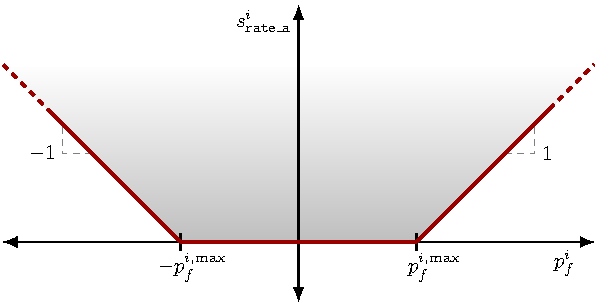
\includegraphics[width=0.8\textwidth]{./figures/softlims}
  \caption{Feasible Region for Branch Flow Violation Constraints}
  \label{fig:softlims}
\end{figure}

\matpower{} implements soft limits for each of the types of constraints listed in Table~\ref{tab:softlimsformulation}, where the formulation for each constraint type is shown.

\begin{table}[!ht]
\centering
\begin{threeparttable}
\caption{Soft Limit Formulation}
\label{tab:softlimsformulation}
\footnotesize
% \begin{tabular}{l p{0.3\textwidth} p{0.4\textwidth}}
\begin{tabular}{lll}
\toprule
name & hard-limit formulation & soft-limit formulation \\ 
\midrule
\code{VMIN}, \code{VMAX}\tnote{\dag} & $v^i_m \geq v^{i,\text{min}}_m $,\quad $v^i_m \leq v^{i,\text{max}}_m$ & $v^i_m + s^i_{\tt{vmin}} \geq v^{i,\text{min}}_m$,\quad $v^i_m - s^i_{\tt{vmax}} \leq v^{i,\text{max}}_m$ \\
%\code{VMAX}\tnote{\dag} &$v^i_m \leq v^{i,\text{max}}_m$ & $v^i_m - s^i_{\tt{vmax}} \leq v^{i,\text{max}}_m$ \\
\code{RATE\_A}\tnote{\ddag} & $\left| f_f^i(\Theta, V_m) \right|  \le f^i_{\text{max}}$ & $\left| f_f^i(\Theta, V_m) \right| - s_{\tt{rate\_a}} \le f^i_{\text{max}}$ \\
& $\left| f_t^i(\Theta, V_m) \right|  \le f^i_{\text{max}}$ & $\left| f_t^i(\Theta, V_m) \right| - s_{\tt{rate\_a}} \le f^i_{\text{max}}$ \\
\code{PMIN}, \code{PMAX} & $p^i_g \geq p^{i,\text{min}}_g$,\quad $p^i_g \leq p^{i,\text{max}}_g$ & $p^i_g + s_{\tt{pmin}} \geq p^{i,\text{min}}_g$,\quad $p^i_g - s_{\tt{pmax}} \leq p^{i,\text{max}}_g$  \\
%\code{PMAX} & $p^i_g \leq p^{i,\text{max}}_g$ &  $p^i_g - s_{\tt{pmax}} \leq p^{i,\text{max}}_g$  \\
\code{QMIN}, \code{QMAX}\tnote{\dag} & $q^i_g \geq q^{i,\text{min}}_g$, \quad $q^i_g \leq q^{i,\text{max}}_g$ &  $q^i_g + s_{\tt{qmin}} \geq q^{i,\text{min}}_g$, \quad $q^i_g - s_{\tt{qmax}} \leq q^{i,\text{max}}_g$ \\
%\code{QMAX}\tnote{\dag} & $q^i_g \leq q^{i,\text{max}}_g$ &  $q^i_g - s_{\tt{qmax}} \leq q^{i,\text{max}}_g$  \\
\code{ANGMIN} & $\theta^i_f - \theta^i_t \geq \Delta\theta^{i,\text{min}}$ & $\theta^i_f - \theta^i_t + s_{\tt{angmin}} \geq \Delta\theta^{i,\text{min}}$  \\
\code{ANGMAX} & $\theta^i_f - \theta^i_t \leq \Delta\theta^{i,\text{max}}$ & $\theta^i_f - \theta^i_t - s_{\tt{angmax}} \leq \Delta\theta^{i,\text{max}}$  \\
\bottomrule
\end{tabular}
\begin{tablenotes}
 \scriptsize
 \item [\dag] {Only applicable for the AC OPF.} 
 \item [\ddag] {Example of a user-defined nonlinear constraint in the AC version.}
\end{tablenotes}
\end{threeparttable}
\end{table}

The parameters for the problem are specified in an additional \code{softlims} field in the \matpower{} case struct \mpc{}.
This field is itself a struct where each sub-field corresponds to the name of one of the limits listed in Table~\ref{tab:softlimsformulation}.
For each of the limits, the input parameters are specified in the fields detailed in Table~\ref{tab:softlimsinput}, with defaults summarized in Table~\ref{tab:softlimsdefaults}.

\begin{table}[!ht]
\centering
\begin{threeparttable}
\caption{Input Data Structures for OPF Soft Limits}
\label{tab:softlimsinput}
\footnotesize
\begin{tabular}{lp{0.8\textwidth}}
\toprule
name & description \\
\midrule
\mpc{} & \matpower{} case struct \\
\code{~~softlims} & additional field in \mpc{} containing OPF soft limit input parameters for the possible limits, each of which is optional.\tnote{*} \\
\code{~~~~<LIM>} & \code{<LIM>} refers to the name of the limit, i.e. one of the following: \code{ANGMIN}, \code{ANGMAX}, \code{RATE\_A}, \code{PMIN}, \code{PMAX}, \code{QMIN}, \code{QMAX}, \code{VMIN}, \code{VMAX}. Each of these is a struct with input parameters defining the soft limits for this type of constraint in the following optional fields (see Table~\ref{tab:softlimsdefaults} for defaults): \\
\code{~~~~~~idx} & $n_\mathrm{sl} \times 1$ vector of row indices for \bus{}, \branch{} or \gen{} matrix, depending on \code{<LIM>}, specifying the elements for which corresponding soft limits are to be applied\tnote{\dag} \\
\code{~~~~~~busnum}\tnote{\ddag} & $n_\mathrm{sl} \times 1$ vector of \emph{external} bus numbers specifying the buses to which soft limits are to be applied\tnote{\dag} \\
\code{~~~~~~cost} & scalar or $n_\mathrm{sl} \times 1$ vector $c_\mathrm{v}$ of linear cost coefficients for limit violation costs \\
\code{~~~~~~hl\_mod}\tnote{\S} & string indicating type of modification to original hard limit: \\
& ~~\begin{tabular}{l @{ -- } p{0.65\textwidth}}
\codeq{none} & do \emph{not} add soft limit, no change to original hard limit \\
\codeq{remove} & add soft limit, relax hard limit by removing it completely \\
\codeq{replace} & add soft limit, relax hard limit by replacing original with value specified in \code{hl\_val} \\
\codeq{scale} & add soft limit, relax hard limit by scaling original by value specified in \code{hl\_val} \\
\codeq{shift} & add soft limit, relax hard limit by shifting original by value specified in \code{hl\_val} \\
\end{tabular} \\
\code{~~~~~~hl\_val}\tnote{\S} & scalar or $n_\mathrm{sl} \times 1$ vector value used to modify hard limit according to \code{hl\_mod}. Ignored for \codeq{none} and \codeq{remove}, required for \codeq{replace}, and optional, with the following defaults, for \codeq{scale} and \codeq{shift}: \\
& ~~\begin{tabular}{l @{ -- } p{0.65\textwidth}}
\codeq{scale} & 2 for positive upper limits or negative lower limits, 0.5 otherwise \\
\codeq{shift} &  0.25 for \code{VMAX} and \code{VMIN}, 10 otherwise \\
\end{tabular} \\
\bottomrule
\end{tabular}
\begin{tablenotes}
 \scriptsize
 \item [*] {For fields not present, the value of the \codeq{opf.softlims.defaults} option determines whether the corresponding limit is unchanged (= 0) or converted (= 1, default) to a soft limit using default values from Table~\ref{tab:softlimsdefaults}.} 
 \item [\dag] {For bus constraints, \code{idx} overrides \code{busnum} if both are provided.} 
 \item [\ddag] {Only applicable for bus constraints, i.e. \code{<LIM>} is \code{VMIN} or \code{VMAX}.} 
 \item [\S] {Any new, relaxed hard limits are implemented via bounds on the violation variables. See Table~\ref{tab:hlmod} for details.}
\end{tablenotes}
\end{threeparttable}
\end{table}


\begin{table}[!ht]
\centering
\begin{threeparttable}
\caption{Default Soft Limit Values}
\label{tab:softlimsdefaults}
\footnotesize
\begin{tabular}{lp{0.75\textwidth}}
\toprule
name & description \\
\midrule
\code{VMIN} & voltage magnitude lower bound \\
\code{~~~~idx}		& all buses \\
\code{~~~~cost}	&  \$100,000/p.u.\tnote{\dag} \\
\code{~~~~hl\_mod}	& \codeq{replace} \\
\code{~~~~hl\_val}	& 0 \\
%
\code{VMAX} 		& voltage magnitude upper bound \\
\code{~~~~idx}		& all buses \\
\code{~~~~cost}	&  \$100,000/p.u.\tnote{\dag} \\
\code{~~~~hl\_mod}	& \codeq{remove} \\
%
\code{RATE\_A} 	& branch flow limit \\
\code{~~~~idx}		& all on-line branches with bounded flow limits  \\
\code{~~~~cost}	&  \$1000/MVA, \$1000/MW, or \$1000/(kA$\cdot V_\mathrm{basekV})$\tnote{\dag} ~where the units depend on \codeq{opf.flow\_lim} \\
\code{~~~~hl\_mod}	& \codeq{remove} \\
%
\code{PMIN} 	 	& generator active power lower bound \\
\code{~~~~idx}		& all on-line generators, excluding dispatchable loads \\
\code{~~~~cost}	&  \$1000/MW\tnote{\dag} \\
\code{~~~~hl\_mod}	& \codeq{replace} \\
\code{~~~~hl\_val}	& 0 if $P^{i,\text{min}}_g \geq 0$, $-\infty$ otherwise \\
%
\code{PMAX}, \code{QMIN}, \code{QMAX} 	 	& generator active power upper bound, reactive power lower/upper bounds \\
\code{~~~~idx}		& all on-line generators, excluding dispatchable loads \\
\code{~~~~cost}	& \$1000/MW or \$1000/MVAr\tnote{\dag} \\
\code{~~~~hl\_mod}	& \codeq{remove} \\
%
\code{ANGMIN}, \code{ANGMAX}   	& branch angle difference lower/upper bounds \\
\code{~~~~idx}		& all on-line branches with angle difference limits, $\Delta\theta$, where $|\Delta\theta| < 360^{\circ}$  \\
\code{~~~~cost}	&  \$1000/deg\tnote{\dag} \\
\code{~~~~hl\_mod}	& \codeq{remove} \\
%
\bottomrule
\end{tabular}
\begin{tablenotes}
 \scriptsize
 \item [\dag] {Unless the maximum marginal cost at $P^\mathrm{max}$ across all online generators, which we call $c_g^\mathrm{max}$, exceeds \$1000/MWh, in which case the numerical value of the default cost is $c_g^\mathrm{max}$ instead of 1000 (or $100 \cdot c_g^\mathrm{max}$ instead of 100,000, for \code{VMIN} or \code{VMAX}).}
 \end{tablenotes}
\end{threeparttable}
\end{table}

Depending on whether the original constraint in \eqref{eq:softlims_infbound} is an upper bound or a lower bound, it can be written as one of the following
\begin{equation}
h^i(x) = \left\{
\begin{aligned}
\; \bar{h}^i(x) - h^{i,\mathrm{lim}} & \qquad \text{(upper bound)} \\
\; h^{i,\mathrm{lim}} - \bar{h}^i(x) & \qquad \text{(lower bound)}
\end{aligned}
\right.
\end{equation}
where $h^{i,\mathrm{lim}}$ is the actual value of the hard limit.
When introducing a soft limit, this original hard limit can be removed completely or modified to have a new value.
\matpower{} provides a several ways of modifying the original hard limit based on fields \code{hl\_mod} (``hard limit modification'') and \code{hl\_val} (``hard limit value'') in the respective limit structures. This new hard limit is implemented via an upper bound on the corresponding violation variable $s^i$.
Table~\ref{tab:hlmod} summarizes the new hard limits and the corresponding bounds on the violation variable as functions of the values of \code{hl\_mod} and \code{hl\_val}.

\begin{table}[!ht]
\centering
\begin{threeparttable}
\caption{Possible Hard-Limit Modifications}
\label{tab:hlmod}
\footnotesize
\begin{tabular}{l c c}
\toprule
\code{h\_mod} & new hard limit $h_\mathrm{new}^{i,\mathrm{lim}}$ & upper bound on violation variable $s^i$ \\
\midrule
\codeq{remove} & $\pm\infty$\tnote{\dag} & $\infty$ \\
\codeq{replace} & $\tt{hl\_val}$       & $ \left|\tt{hl\_val} -  h_\mathrm{orig}^{i,\mathrm{lim}}\right|$ \\
\codeq{scale}    & $\tt{hl\_val}\cdot h_\mathrm{orig}^{i,\mathrm{lim}}$	& $\left|(\tt{hl\_val} - 1) \cdot h_\mathrm{orig}^{i,\mathrm{lim}}\right|$ \\
\codeq{shift}	&$h_\mathrm{orig}^{i,\mathrm{lim}} \pm \tt{hl\_val}$\tnote{\dag} &  $\code{hl\_val}$ \\
\bottomrule
\end{tabular}
\begin{tablenotes}
 \scriptsize
 \item [\dag] {Plus sign for upper bounds and minus sign for lower bounds.}
 \end{tablenotes}
\end{threeparttable}
\end{table}

Unspecified limits in the \code{mpc.softlims} input parameters are handled differently, depending on the value of the \matpower{} option \codeq{opf.softlims.default} (see Table~\ref{tab:opfoptions2}). 

\begin{itemize}
	\item If the \code{opf.softlims.default} option is 1 (default), each limit not explicitly specified, whether missing in \code{mpc.softlims} or present but empty, will be initialized as in Table~\ref{tab:softlimsdefaults}. 
	\item If the \code{opf.softlims.default} option is 0, limits that are missing in \code{mpc.softlims} are treated as though specified with \code{hl\_mod} = \codeq{none}, that is, they are not converted to soft limits at all. On the other hand, the default soft limits of Table~\ref{tab:softlimsdefaults} are still applied to any limit that is present in \code{mpc.softlims} but empty.
	For example, \code{mpc.softlims.RATE\_A = struct()} would result in the default soft branch limits being applied.
\end{itemize}

Soft limit outputs, summarized in Table~\ref{tab:softlimsoutput}, include the amount and cost of any overloads, that is, violations of the original hard limits. These can be found as additional fields, \code{overload} and \code{ov\_cost}, under each limit in \code{results.softlims}. The Kuhn-Tucker multipliers on the soft limit constraints are also included in the usual columns of the corresponding matrix in the \results{}, e.g. \code{bus(:, MU\_VMAX)}, \code{branch(:, MU\_SF)}, etc.
When there are no violations, these shadow prices are the same as if hard limits were imposed.
When there is a violation, they are equal to the cost $c_\mathrm{v}$ associated with the violation variable, except in the case where a modified hard limit is also binding, in which case it also reflects the shadow price on this modified hard constraint.

\begin{table}[!ht]
\centering
\begin{threeparttable}
\caption{Output Data Structures for OPF Soft Limits}
\label{tab:softlimsoutput}
\footnotesize
\begin{tabular}{lp{0.68\textwidth}}
\toprule
name & description \\
\midrule
\results{} & \matpower{} case struct \\
\code{~~softlims} & additional field in \results{} containing OPF soft limit outputs for each limit type \\
\code{~~~~<LIM>} & \code{<LIM>} refers to the name of the limit, i.e. one of the following: \code{ANGMIN}, \code{ANGMAX}, \code{RATE\_A}, \code{PMIN}, \code{PMAX}, \code{QMIN}, \code{QMAX}, \code{VMIN}, \code{VMAX}. Each of these is a struct with the following output fields: \\
\code{~~~~~~overload}\tnote{\dag} & $n_{b/l/g} \times 1$ vector of overload quantities for this limit (amount of original hard limit violation) \\
\code{~~~~~~ov\_cost}\tnote{\dag} & $n_{b/l/g} \times 1$ vector of overload penalty costs for this limit \\
\code{~~branch(:, MU\_ANGMIN)} & Kuhn-Tucker multipliers on angle difference lower bounds\tnote{\ddag} \\
\code{~~branch(:, MU\_ANGMAX)} & Kuhn-Tucker multipliers on angle difference upper bounds\tnote{\ddag} \\
\code{~~branch(:, MU\_SF)} & Kuhn-Tucker multipliers on branch flow limits (\emph{from} end)\tnote{\ddag} \\
\code{~~branch(:, MU\_ST)} & Kuhn-Tucker multipliers on branch flow limits (\emph{to} end)\tnote{\ddag} \\
\code{~~gen(:, MU\_PMIN)} & Kuhn-Tucker multipliers on active gen lower bounds\tnote{\ddag} \\
\code{~~gen(:, MU\_PMAX)} & Kuhn-Tucker multipliers on active gen upper bounds\tnote{\ddag} \\
\code{~~gen(:, MU\_QMIN)} & Kuhn-Tucker multipliers on reactive gen lower bounds\tnote{\ddag} \\
\code{~~gen(:, MU\_QMAX)} & Kuhn-Tucker multipliers on reactive gen upper bounds\tnote{\ddag} \\
\code{~~bus(:, MU\_VMIN)} & Kuhn-Tucker multipliers on voltage magnitude lower bounds\tnote{\ddag} \\
\code{~~bus(:, MU\_VMAX)} & Kuhn-Tucker multipliers on voltage magnitude upper bounds\tnote{\ddag} \\
\bottomrule
\end{tabular}
\begin{tablenotes}
 \scriptsize
 \item [\dag] {The dimensions of \code{overload} and \code{ov\_cost} correspond to all buses, branches or generators (depending on \code{<LIM>}), not just those whose limits were converted to soft limits. Entries corresponding to those not included (implicitly or explicitly) in \code{idx} are set to zero.}
 \item [\dag] {For limits that have been converted to soft limits, these are the shadow prices on the soft limit constraints. When there is no violation of the soft limit, this shadow price is the same as it would be for the original hard limit. When there is a violation, it is equal to the corresponding user-supplied violation cost $c_\mathrm{v}^i$, unless an updated hard constraint is also binding.}
\end{tablenotes}
\end{threeparttable}
\end{table}

\clearpage
See \code{help toggle\_softlims} for more information on this extension. Examples of using this extension can be found in \code{t\_opf\_softlims}.
Running a case that includes the default soft limits is as simple as loading the case, turning on the extension and running it. Unlike with the reserves extension, \matpower{} does not currently have a wrapper function to automate this.
\begin{Code}
mpc = loadcase('case2383wp');
mpc = toggle_softlims(mpc, 'on');
results = runopf(mpc, mpopt);
\end{Code}

%%------------------------------------------
\clearpage
\section{Unit De-commitment Algorithm}
\label{sec:decommitment}

The standard OPF formulation described in the previous section has no mechanism for completely shutting down generators which are very expensive to operate. Instead they are simply dispatched at their minimum generation limits. \matpower{} includes the capability to run an optimal power flow combined with a unit de-commitment for a single time period, which allows it to shut down these expensive units and find a least cost commitment and dispatch. To run this for \code{case30}, for example, type:
\begin{Code}
>> runuopf('case30')
\end{Code}
By default, \code{runuopf} is based on the AC optimal power flow problem. To run a DC OPF, the \code{model} option must be set to \codeq{DC}. For convenience, \matpower{} provides a function \code{runduopf} which is simply a wrapper that sets the \code{model} option to \codeq{DC} before calling \code{runuopf}.

\matpower{} uses an algorithm similar to dynamic programming to handle the de-commitment. It proceeds through a sequence of stages, where stage $N$ has $N$ generators shut down, starting with $N = 0$, as follows:
\begin{enumerate}[\bfseries Step 1:] % requires package paralist
\item Begin at stage zero ($N = 0$), assuming all generators are on-line with all limits in place.

\item If the sum of the minimum generation limits for all on-line generators is less than the total system demand, then go to Step~\ref{step:firstopf}. Otherwise, go to the next stage, $N = N + 1$, shut down the generator whose average per-MW cost of operating at its minimum generation limit is greatest and repeat Step~\ref{step:pminfeasible}.\label{step:pminfeasible}

\item Solve a normal OPF. Save the solution as the current best.\label{step:firstopf}

\item Go to the next stage, $N = N + 1$. Using the best solution from the previous stage as the base case for this stage, form a candidate list of generators with minimum generation limits binding.
If there are no candidates, skip to Step~\ref{step:last}.\label{step:next}

\item For each generator on the candidate list, solve an OPF to find the total system cost with this generator shut down. Replace the current best solution with this one if it has a lower cost.
If any of the candidate solutions produced an improvement, return to Step~\ref{step:next}.

\item Return the current best solution as the final solution. \label{step:last}
\end{enumerate}

It should be noted that the method employed here is simply a heuristic. It does not guarantee that the least cost commitment of generators will be found. It is also rather computationally expensive for larger systems and was implemented as a simple way to allow an OPF-based ``smart-market'', such as described in Appendix~\ref{app:smartmarket}, the option to reject expensive offers while respecting the minimum generation limits on generators.


%%------------------------------------------
\clearpage
\section{Miscellaneous \matpower{} Functions}
\label{sec:miscfunctions}

This section describes a number of additional \matpower{} functions that users may find useful. The descriptions here are simply brief summaries, so please use the \matlab{} \code{help} function to get the full details on each function.

\subsection{Input/Output Functions}
\label{sec:io_funcs}

\subsubsection{\tt loadcase}
\label{sec:loadcase}

\begin{Code}
  mpc = loadcase(casefile)
\end{Code}

The \code{loadcase} function provides the canonical way of loading a \matpower{} case from a file or struct. It takes as input either a struct or the name of an M-file or MAT-file in the \matlab{} path (\code{casefile}) and returns a standard \matpower{} case struct (\mpc{}). It can also convert from the older version 1 case file format to the current format. This function allows a case to be loaded, and potentially modified, before calling one of the main simulation functions such as \code{runpf} or \code{runopf}.

\subsubsection{\tt savecase}

\begin{Code}
  savecase(fname, mpc)
  savecase(fname, mpc, version)
  savecase(fname, comment, mpc)
  savecase(fname, comment, mpc, version)
  fname = savecase(fname, ...)
\end{Code}

The \code{savecase} function writes out a \matpower{} case file, given a name for the file to be created or overwritten (\code{fname}), and a \matpower{} case struct (\mpc{}). If \code{fname} ends with \codeq{.mat} it saves the case as a MAT-file, otherwise it saves it as an M-file. Optionally returns the filename, with extension added if necessary. The optional \code{comment} argument is either string (single line comment) or a cell array of strings which are inserted as comments in the help section of the file. If the optional \code{version} argument is \codeq{1} it will modify the data matrices to version 1 format before saving.

\subsubsection{\tt cdf2mpc}

\begin{Code}
  mpc = cdf2mpc(cdf_file_name)
  mpc = cdf2mpc(cdf_file_name, verbose)
  mpc = cdf2mpc(cdf_file_name, mpc_name)
  mpc = cdf2mpc(cdf_file_name, mpc_name, verbose)
  [mpc, warnings] = cdf2mpc(cdf_file_name, ...)
\end{Code}

The \code{cdf2mpc} function converts an IEEE Common Data Format (CDF) data file into a \matpower{} case struct. Given an optional file name \code{mpc\_name}, it can save the converted case to a \matpower{} case file. Warnings generated during the conversion process can be optionally returned in the \code{warnings} argument.

Since the IEEE CDF format does not contain all of the data needed to run an optimal power flow, some data, such as voltage limits, generator limits and generator costs are created by \code{cdf2mpc}. See \code{help cdf2mpc} for details.

\subsubsection{\tt psse2mpc}

\begin{Code}
  mpc = psse2mpc(rawfile_name)
  mpc = psse2mpc(rawfile_name, verbose)
  mpc = psse2mpc(rawfile_name, verbose, rev)
  mpc = psse2mpc(rawfile_name, mpc_name)
  mpc = psse2mpc(rawfile_name, mpc_name, verbose)
  mpc = psse2mpc(rawfile_name, mpc_name, verbose, rev)
  [mpc, warnings] = psse2mpc(rawfile_name, ...)
\end{Code}

The \code{psse2mpc} function converts a PSS/E RAW data file into a \matpower{} case struct. Given an optional file name \code{mpc\_name}, it can save the converted case to a \matpower{} case file. Warnings generated during the conversion process can be optionally returned in the \code{warnings} argument. By default, \code{psse2mpc} attempts to determine the revision of the PSS/E RAW file from the contents, but the user can specify an explicit revision number to use in the optional \code{rev} argument.

\clearpage
\subsubsection{\tt save2psse}

\begin{Code}
  save2psse(fname, mpc)
  fname_out = save2psse(fname, mpc)
\end{Code}

The \code{save2psse} function saves a \matpower{} case struct \code{mpc} as a PSS/E RAW file. The \code{fname} parameter is a string containing the name of the file to be created or overwritten. If \code{fname} does not include a file extension, codeq{.raw} will be added. Optionally returns the, possibly updated, filename. Currently exports to RAW format Rev 33.


\subsection{System Information}

\subsubsection{\tt case\_info}

\begin{Code}
  case_info(mpc)
  case_info(mpc, fd)
  [groups, isolated] = case_info(mpc)
\end{Code}

The \code{case\_info} function prints out detailed information about a \matpower{} case, including connectivity information, summarizing the generation, load and other data by interconnected island. It can optionally print the output to an open file, whose file identifier (as returned by \code{fopen}) is specified in the optional second parameter \code{fd}. Optional return arguments include \code{groups} and \code{isolated} buses, as returned by the \code{find\_islands} function.

\subsubsection{\tt compare\_case}

\begin{Code}
  compare_case(mpc1, mpc2)
\end{Code}

Compares the \bus{}, \branch{} and \gen{} matrices of two \matpower{} cases and prints a summary of the differences. For each column of the matrix it prints the maximum of any non-zero differences.

\clearpage
\subsubsection{\tt find\_islands}

\begin{Code}
  groups = find_islands(mpc)
  [groups, isolated] = find_islands(mpc)
\end{Code}

The \code{find\_islands} function returns the islands in a network. The return value \code{groups} is a cell array of vectors of the bus indices for each island. The second and optional return value \code{isolated} is a vector of indices of isolated buses that have no connecting branches.

\subsubsection{\tt get\_losses}

\begin{Code}
  loss = get_losses(results)
  loss = get_losses(baseMVA, bus, branch)

  [loss, chg] = get_losses(results)
  [loss, fchg, tchg] = get_losses(results)
  [loss, fchg, tchg, dloss_dv] = get_losses(results)
  [loss, fchg, tchg, dloss_dv, dchg_dvm] = get_losses(results)
\end{Code}

The \code{get\_losses} function computes branch series losses, and optionally reactive injections from line charging, as functions of bus voltages and branch parameters, using the following formulae for a branch, as described in Section~\ref{sec:branch}, connecting bus~$f$ to bus~$t$:

\begin{align}
\mathrm{loss}_i &= \frac{\left|\frac{v_f}{\tau e^{j\theta_{\rm shift}}} - v_t\right|^2}{r_s - j x_s} \\
f_{\rm chg} &= \left|\frac{v_f}{\tau e^{j\theta_{\rm shift}}}\right|^2 \frac{b_c}{2} \\
t_{\rm chg} &= \left|v_t\right|^2 \frac{b_c}{2}
\end{align}

It can also optionally compute the partial derivatives of the line losses and reactive charging injections with respect to voltage angles and magnitudes.

\clearpage
\subsubsection{\tt margcost}
\begin{Code}
  marginalcost = margcost(gencost, Pg)
\end{Code}

The \code{margcost} function computes the marginal cost for generators given a matrix in \gencost{} format and a column vector or matrix of generation levels. The return value has the same dimensions as \code{Pg}. Each row of \gencost{} is used to evaluate the cost at the output levels specified in the corresponding row of \code{Pg}. The rows of \gencost{} can specify either polynomial or piecewise linear costs and need not be uniform.

\subsubsection{\tt isload}
\begin{Code}
  TorF = isload(gen)
\end{Code}

The \code{isload} function returns a column vector of 1's and 0's. The 1's correspond to rows of the \gen{} matrix which represent dispatchable loads. The current test is $P_{\rm min} < 0$ and $P_{\rm max} = 0$.

\subsubsection{\tt loadshed}
\begin{Code}
  shed = loadshed(gen)
  shed = loadshed(gen, ild)
\end{Code}

The \code{loadshed} function returns a column vector of MW curtailments of dispatchable loads, computed as the difference between the \code{PG} and \code{PMIN} values in the corresponding rows of the \gen{} matrix. The optional \code{ild} argument is a column vector of generator indices to the dispatchable loads of interest.

\subsubsection{\tt printpf}
\begin{Code}
  printpf(results, fd, mpopt)
\end{Code}

The \code{printpf} function prints power flow and optimal power flow results, as returned to \code{fd}, a file identifier which defaults to STDOUT (the screen). The details of what gets printed are controlled by an optional \matpower{} options struct \code{mpopt}.

\subsubsection{\tt total\_load}
\begin{Code}
  Pd = total_load(mpc)
  Pd = total_load(mpc, load_zone, opt, mpopt)
  Pd = total_load(bus)
  Pd = total_load(bus, gen, load_zone, opt, mpopt)
  [Pd, Qd] = total_load(...)
\end{Code}

The \code{total\_load} function returns a vector of total load in each load zone. The \code{opt} argument controls whether it includes fixed loads, dispatchable loads or both, and for dispatchable loads, whether to use the nominal or realized load values. The \code{load\_zone} argument defines the load zones across which loads will be summed. It uses the \code{BUS\_AREA} column (7) of the \bus{} matrix by default. The string value \codeq{all} can be used to specify a single zone including the entire system. The reactive demands are also optionally available as an output.

\subsubsection{\tt totcost}
\begin{Code}
  totalcost = totcost(gencost, Pg)
\end{Code}

The \code{totcost} function computes the total cost for generators given a matrix in \gencost{} format and a column vector or matrix of generation levels. The return value has the same dimensions as \code{Pg}. Each row of \gencost{} is used to evaluate the cost at the output levels specified in the corresponding row of \code{Pg}. The rows of \gencost{} can specify either polynomial or piecewise linear costs and need not be uniform.


\subsection{Modifying a Case}

\subsubsection{\tt extract\_islands}
\begin{Code}
  mpc_array = extract_islands(mpc)
  mpc_array = extract_islands(mpc, groups)
  mpc_k = extract_islands(mpc, k)
  mpc_k = extract_islands(mpc, groups, k)
  mpc_k = extract_islands(mpc, k, custom)
  mpc_k = extract_islands(mpc, groups, k, custom)
\end{Code}

The \code{extract\_islands} function extracts individual islands in a network that is not fully connected. The original network is specified as a \matpower{} case struct (\mpc{}) and the result is returned as a cell array of case structs, or as a single case struct. Supplying the optional \code{group} avoids the need to traverse the network again, saving time on large systems. A final optional argument \code{custom} is a struct that can be used to indicate custom fields of \mpc{} from which to extract data corresponding to buses generators, branches or DC lines.

\subsubsection{\tt load2disp}
\begin{Code}
  mpc = load2disp(mpc0)
  mpc = load2disp(mpc0, fname)
  mpc = load2disp(mpc0, fname, idx)
  mpc = load2disp(mpc0, fname, idx, voll)
\end{Code}

The \code{load2disp} function takes a \matpower{} case \code{mpc0}, converts fixed loads to dispatchable loads, curtailable at a specific price, and returns the resulting case struct \mpc{}. It can optionally save the resulting case to a file (\code{fname}), convert loads only at specific buses (\code{idx}), and set the value of lost load (\code{voll}) to be used as the curtailment price (default is \$5,000/MWh).

\subsubsection{\tt modcost}
\begin{Code}
  newgencost = modcost(gencost, alpha)
  newgencost = modcost(gencost, alpha, modtype)
\end{Code}

The \code{modcost} function can be used to modify generator cost functions by shifting or scaling them, either horizontally or vertically. The \code{alpha} argument specifies the numerical value of the modification, and \code{modtype} defines the type of modification as a string that takes one of the following values: \codeq{SCALE\_F} (default), \codeq{SCALE\_X}, \codeq{SHIFT\_F}, or \codeq{SHIFT\_X}.

\subsubsection{\tt scale\_load}
\begin{Code}
  mpc = scale_load(load, mpc)
  mpc = scale_load(load, mpc, load_zone)
  mpc = scale_load(load, mpc, load_zone, opt)
  bus = scale_load(load, bus)
  [bus, gen] = scale_load(load, bus, gen, load_zone, opt)
  [bus, gen, gencost] = ...
      scale_load(load, bus, gen, load_zone, opt, gencost)
\end{Code}

The \code{scale\_load} function is used to scale active (and optionally reactive) loads in each zone by a zone-specific ratio, i.e. $R(k)$ for zone~$k$. The amount of scaling for each zone, either as a direct scale factor or as a target quantity, is specified in \code{load}. The load zones are defined by \code{load\_zone}, and \code{opt} specifies the type of scaling (factor or target quantity) and which loads are affected (active, reactive or both and fixed, dispatchable or both). The costs (\gencost{}) associated with dispatchable loads can also be optionally scaled with the loads.

\subsubsection{\tt apply\_changes}
\label{sec:apply_changes}

\begin{Code}
  mpc_modified = apply_changes(label, mpc_original, chgtab)
\end{Code}

The \code{apply\_changes} function implements a general mechanism to apply a set of changes to a base \matpower{} case. This can be used, for example, to define and apply a set of contingencies. There are three basic types of changes, those that replace old values with new ones, those that scale old values by some factor, and those that add a constant to existing values.

The \emph{change table} matrix, \code{chgtab}, specifies modifications to be applied to an existing case. These modifications are grouped into sets, designated \emph{change sets}, that are always applied as a group. A change set consists of one or more changes, each specified in a separate row in the \code{chgtab}, where the rows share a common \code{label} (integer ID).

For example, $n_c$ change sets can be used to define $n_c$ contingencies via a single \code{chgtab} with many rows, but only $n_c$ unique labels. The \code{chgtab} also optionally specifies a probability $\pi_k$ of occurance associated with change set $k$. Table~\ref{tab:chgtab} summarizes the meaning of the data in each column of \code{chgtab}. All of the names referenced in Tables~\ref{tab:chgtab} through \ref{tab:ctcol} are defined as constants by the \code{idx\_ct} function. Type \code{help idx\_ct} at the \matlab{} prompt for more details. Use of the named constants when constructing a \code{chgtab} matrix is encouraged to improve readability.

\begin{table}[!ht]
%\renewcommand{\arraystretch}{1.2}
\centering
\begin{threeparttable}
\caption{Columns of \code{chgtab}}
\label{tab:chgtab}
\footnotesize
\begin{tabular}{lcl}
\toprule
name & column & description \\
\midrule
\code{CT\_LABEL}	& 1 & change set label, unique for each change set (integer)	\\
\code{CT\_PROB}		& 2 & change set probability (number between 0 and 1)\tnote{\dag} 	\\
\code{CT\_TABLE}	& 3 & type of table to be modified (see Table~\ref{tab:cttable} for possible values)	\\
\code{CT\_ROW}		& 4 & row index of data to be modified, 0 means all rows,	\\
						&& for area-wide changes this is the area index, rather than row index	\\
\code{CT\_COL}		& 5 & column index of data to be modified (see Table~\ref{tab:ctcol} for exceptions)	\\
\code{CT\_CHGTYPE}	& 6 & type of change, e.g. replace, scale or add (see Table~\ref{tab:ctchgtype} for details)	\\
\code{CT\_NEWVAL}	& 7 & new value used to replace or modify existing data	\\
\bottomrule
\end{tabular}
\begin{tablenotes}
 \scriptsize
 \item [\dag] {The change set probability $\pi_k$ is taken from this column of the \emph{first} row for change set~$k$.}
\end{tablenotes}
\end{threeparttable}
\end{table}

The value in the \code{CT\_TABLE} column of \code{chgtab} defines which data table is to be modified and the options are given in Table~\ref{tab:cttable}. With the exception of load and certain generator cost changes, each individual change record specifies modification(s) to a single column of a particular data matrix, either \bus{}, \gen{}, \branch{} or \gencost{}. Some are changes to that column for an individual row in the matrix (or all rows, if the row index is set to 0), while others are area-wide changes that modify all rows corresponding to the specified area.\footnote{Areas are defined by the \code{BUS\_AREA} column of the \bus{} matrix.}

Load changes are special and may modify multiple columns of the \bus{} and/or \gen{} tables. They offer a more flexible and convenient means of specifying modifications to loads (fixed, dispatchable, real and/or reactive) than directly including individual change specifications for each of the corresponding entries in the \bus{} and \gen{} matrices. The row indices for load changes refer to bus numbers.

In addition to the normal direct modifications for generator cost parameters, there is also the option to scale or shift an entire cost function, either vertically or horizontally. This is often more convenient than manipulating the individual cost parameters directly, especially when dealing with a mix of polynomial and piecewise linear generator costs.

\begin{table}[!ht]
%\renewcommand{\arraystretch}{1.2}
\centering
\begin{threeparttable}
\caption{Values for \code{CT\_TABLE} Column}
\label{tab:cttable}
\footnotesize
\begin{tabular}{lcl}
\toprule
name & value & description \\
\midrule
\code{CT\_TBUS}			& 1  & \bus{} table	\\
\code{CT\_TGEN}			& 2  & \gen{} table	\\
\code{CT\_TBRCH}		& 3  & \branch{} table	\\
\code{CT\_TAREABUS}		& 4  & area-wide change in \bus{} table	\\
\code{CT\_TAREAGEN}		& 5  & area-wide change in \gen{} table	\\
\code{CT\_TAREABRCH}	& 6  & area-wide change in \branch{} table	\\
\code{CT\_TLOAD}		& 7  & per bus load change\tnote{\dag}	\\
\code{CT\_TAREALOAD}	& 8  & area-wide load change\tnote{\dag}	\\
\code{CT\_TGENCOST}		& 9  & \gencost{} table	\\
\code{CT\_TAREAGENCOST}	& 10 & area-wide change in \gencost{} table	\\
\bottomrule
\end{tabular}
\begin{tablenotes}
 \scriptsize
 \item [\dag] {Preferred method of modifying load, as opposed to manipulating \bus{} and \gen{} tables directly.}
\end{tablenotes}
\end{threeparttable}
\end{table}

Normally, the \code{CT\_COL} column contains the column index of the entry or entries in the data tables to be modified. And the \code{CT\_CHGTYPE} and \code{CT\_NEWVAL} columns specify, respectively, the type of change (replacement, scaling or adding) and the corresponding replacement value, scale factor or constant to add, as shown in Table~\ref{tab:ctchgtype}.


\begin{table}[!ht]
%\renewcommand{\arraystretch}{1.2}
\centering
\begin{threeparttable}
\caption{Values for \code{CT\_CHGTYPE} Column}
\label{tab:ctchgtype}
\footnotesize
\begin{tabular}{lcl}
\toprule
name & value & description \\
\midrule
\code{CT\_REP}	& 1 & replace old value by new one in \code{CT\_NEWVAL} column	\\
\code{CT\_REL}	& 2 & scale old value by factor in \code{CT\_NEWVAL} column	\\
\code{CT\_ADD}	& 3 & add value in \code{CT\_NEWVAL} column to old value	\\
\bottomrule
\end{tabular}
\end{threeparttable}
\end{table}

For load changes, the \code{CT\_COL} column is not a column index, but rather a code that defines which loads at the specified bus(es) are to be modified, with the ability to select fixed loads only, dispatchable loads only or both, and for each whether or not to include the reactive load in the change. Similarly, the \code{CT\_COL} column for generator cost modifications can be set to a special code to indicate a scaling or shifting of the entire corresponding cost function(s). The various options for the \code{CT\_COL} column are summarized in Table~\ref{tab:ctcol}.

\begin{table}[!ht]
%\renewcommand{\arraystretch}{1.2}
\centering
\begin{threeparttable}
\caption{Values for \code{CT\_COL} Column}
\label{tab:ctcol}
\footnotesize
\begin{tabular}{llcl}
\toprule
& name & value & description \\
\midrule
\multicolumn{4}{l}{\emph{for \code{CT\_TABLE} column = \code{CT\_TLOAD} or \code{CT\_TAREALOAD}}} \\
& \code{CT\_LOAD\_ALL\_PQ}	& 1  & modify all (fixed \& dispatchable) loads, active and reactive	\\
& \code{CT\_LOAD\_FIX\_PQ}	& 2  & modify fixed loads, active and reactive	\\
& \code{CT\_LOAD\_DIS\_PQ}	& 3  & modify dispatchable loads, active and reactive	\\
& \code{CT\_LOAD\_ALL\_P}	& 4  & modify all (fixed \& dispatchable) loads, active power only	\\
& \code{CT\_LOAD\_FIX\_P}	& 5  & modify fixed loads, active power only	\\
& \code{CT\_LOAD\_DIS\_P}	& 6  & modify dispatchable loads, active power only	\\
\midrule
\multicolumn{4}{l}{\emph{for \code{CT\_TABLE} column = \code{CT\_TGENCOST} or \code{CT\_TAREAGENCOST}}} \\
& \code{CT\_MODCOST\_F}	& -1  & scales or shifts the cost function vertically\tnote{\dag}	\\
& \code{CT\_MODCOST\_X}	& -2  & scales or shifts the cost function horizontally\tnote{\dag}	\\
\midrule
\multicolumn{4}{l}{\emph{otherwise}\tnote{\ddag}} \\
& & $n$  & index of column in data matrix to be modified	\\
\bottomrule
\end{tabular}
\begin{tablenotes}
 \scriptsize
 \item [\dag] {Use \code{CT\_CHGTYPE} column = \code{CT\_REL} to scale the cost and \code{CT\_ADD} to shift the cost.}
 \item [\ddag] {Can also be used for \code{CT\_TGENCOST} or \code{CT\_TAREAGENCOST} in addition to the special codes above.}
\end{tablenotes}
\end{threeparttable}
\end{table}

\clearpage
For example, setting up a \code{chgtab} matrix for the following four scenarios could be done as shown below.

\begin{enumerate}
\item Turn off generator 2 (\emph{10\% probability}).
\item Reduce the line rating of all lines to 95\% of their nominal values (\emph{0.2\% probability}).
\item Scale all loads in area 2 (real \& reactive, fixed \& dispatchable)
       up by 10\% (\emph{0.1\% probability}).
\item Decrease capacity of generator 3 \emph{and} shift its cost function to the left both by 10 MW (\emph{5\% probability}).
\end{enumerate}

\begin{Code}
chgtab = [ ...
	1   0.1   CT_TGEN       2  GEN_STATUS     CT_REP    0;
	2   0.002 CT_TBRCH      0  RATE_A         CT_REL    0.95;
	3   0.001 CT_TAREALOAD  2  CT_LOAD_ALL_PQ CT_REL    1.1;
	4   0.05  CT_TGEN       3  PMAX           CT_ADD  -10;
	4   0.05  CT_TGENCOST   3  CT_MODCOST_X   CT_ADD  -10;
 ];
\end{Code}

A change table can be used to easily create modified cases from an existing base case with the \code{apply\_changes} function. Given the \code{chgtab} from the example above, a new case with all lines derated by 5\% can easily be created from an existing case \mpc{} with the following line of code.
\begin{Code}
mpc_new = apply_changes(2, mpc, chgtab);
\end{Code}

\subsubsection{\tt savechgtab}
\begin{Code}
  savechgtab(fname, chgtab)
  savechgtab(fname, chgtab, warnings)
  fname = savechgtab(fname, ...)
\end{Code}

This function can be used to save a \emph{change table} matrix, \code{chgtab}, to a file specified by \code{fname}. If the \code{fname} string ends with \codeq{.mat} it saves \code{chgtab} and \code{warnings} to a MAT-file as the variables \code{chgtab} and \code{warnings}, respectively. Otherwise, it saves an M-file function that returns the \code{chgtab}, with the optional \code{warnings} included in the comments, where \code{warnings} is a cell array of warning messages such as those returned by \code{pssecon2chgtab}.

\subsection{Conversion between External and Internal Numbering}

\subsubsection{{\tt ext2int}, {\tt int2ext}}
\label{sec:ext2int}

\begin{Code}
  mpc_int = ext2int(mpc_ext)
  mpc_int = ext2int(mpc_ext, mpopt)
  mpc_ext = int2ext(mpc_int)
  mpc_ext = int2ext(mpc_int, mpopt)
\end{Code}

These functions convert a \matpower{} case struct from external to internal, and from internal to external numbering, respectively. \code{ext2int} first removes all isolated buses, off-line generators and branches, and any generators or branches connected to isolated buses. Then the buses are renumbered consecutively, beginning at 1.\footnote{In \matpower{} versions 4 through 7.0b1, \code{ext2int} also sorted the generators by increasing internal bus number, but beginning with version 7.0, the order of on-line generators is left unmodified.} Any \codeq{ext2int} callback routines registered in the case are also invoked automatically. All of the related indexing information and the original data matrices are stored in an \codeq{order} field in the struct to be used later by \code{int2ext} to perform the reverse conversions. If the case is already using internal numbering it is returned unchanged. The optional \matpower{} options struct (\code{mpopt}) input argument is only needed in conjunction with callback routines that depend on it, e.g. when \code{toggle\_softlims} is on.

\subsubsection{{\tt e2i\_data}, {\tt i2e\_data}}

\begin{Code}
  val = e2i_data(mpc, val, ordering)
  val = e2i_data(mpc, val, ordering, dim)
  val = i2e_data(mpc, val, oldval, ordering)
  val = i2e_data(mpc, val, oldval, ordering, dim)
\end{Code}

These functions can be used to convert other data structures from external to internal indexing and vice versa. When given a case struct (\mpc{}) that has already been converted to internal indexing, \code{e2i\_data} can be used to convert other data structures as well by passing in 2 or 3 extra parameters in addition to the case struct. If the value passed in the second argument (\code{val}) is a column vector or cell array, it will be converted according to the \code{ordering} specified by the third argument (described below). If \code{val} is an $n$-dimensional matrix or cell array, then the optional fourth argument (\code{dim}, default = 1) can be used to specify which dimension to reorder. The return value in this case is the value passed in, converted to internal indexing.

The third argument, \code{ordering}, is used to indicate whether the data corresponds to bus-, gen- or branch-ordered data. It can be one of the following three strings: \codeq{bus}, \codeq{gen} or \codeq{branch}. For data structures with multiple blocks of data, ordered by bus, gen or branch, they can be converted with a single call by specifying \code{ordering} as a cell array of strings.

Any extra elements, rows, columns, etc. beyond those indicated in \code{ordering}, are not disturbed.

The function \code{i2e\_data} performs the opposite conversion, from internal back to external indexing. It also assumes that \mpc{} is using internal indexing, and the only difference is that it also includes an \code{oldval} argument used to initialize the return value before converting \code{val} to external indexing. In particular, any data corresponding to off-line gens or branches or isolated buses or any connected gens or branches will be taken from \code{oldval}, with \code{val} supplying the rest of the returned data.

\subsubsection{{\tt e2i\_field}, {\tt i2e\_field}}

\begin{Code}
  mpc = e2i_field(mpc, field, ordering)
  mpc = e2i_field(mpc, field, ordering, dim)
  mpc = i2e_field(mpc, field, ordering)
  mpc = i2e_field(mpc, field, ordering, dim)
\end{Code}

These functions can be used to convert additional fields in \mpc{} from external to internal indexing and vice versa. When given a case struct that has already been converted to internal indexing, \code{e2i\_field} can be used to convert other fields as well by passing in 2 or 3 extra parameters in addition to the case struct.

The second argument (\code{field}) is a string or cell array of strings, specifying a field in the case struct whose value should be converted by a corresponding call to \code{e2i\_data}. The field can contain either a numeric or a cell array. The converted value is stored back in the specified field, the original value is saved for later use and the updated case struct is returned. If \code{field} is a cell array of strings, they specify nested fields.

The third and optional fourth arguments (\code{ordering} and \code{dim}) are simply passed along to the call to \code{e2i\_data}.

Similarly, \code{i2e\_field} performs the opposite conversion, from internal back to external indexing. It also assumes that \mpc{} is using internal indexing and utilizes the original data stored by \code{e2i\_field}, calling \code{i2e\_data} to do the conversion work.

\clearpage
\subsection{Forming Standard Power Systems Matrices}

\subsubsection{\tt makeB}
\begin{Code}
  [Bp, Bpp] = makeB(mpc, alg)
  [Bp, Bpp] = makeB(baseMVA, bus, branch, alg)
\end{Code}

The \code{makeB} function builds the two matrices $B'$  and $B''$ used in the fast-decoupled power flow. The \code{alg}, which can take values \codeq{FDXB} or \codeq{FDBX}, determines whether the matrices returned correspond to the XB or BX version of the fast-decoupled power flow.
Bus numbers must be consecutive beginning at 1 (i.e. internal ordering).

\subsubsection{\tt makeBdc}
\begin{Code}
  [Bbus, Bf, Pbusinj, Pfinj] = makeBdc(mpc)
  [Bbus, Bf, Pbusinj, Pfinj] = makeBdc(baseMVA, bus, branch)
\end{Code}

The \code{} function builds the $B$ matrices, $B_{dc}$ (\code{Bbus}) and $B_f$ (\code{Bf}), and phase shift injections, $P_{dc}$ (\code{Pbusinj}) and $P_{f,\mathrm{shift}}$ (\code{Pfinj}), for the DC power flow model as described in \eqref{eq:Pf} and \eqref{eq:dcpf2}.
Bus numbers must be consecutive beginning at 1 (i.e. internal ordering).


\subsubsection{\tt makeJac}
\begin{Code}
  J = makeJac(mpc)
  J = makeJac(mpc, fullJac)
  [J, Ybus, Yf, Yt] = makejac(mpc)
\end{Code}

The \code{makeJac} function forms the power flow Jacobian and, optionally, the system admittance matrices. Bus numbers in the input case must be consecutive beginning at 1 (i.e. internal indexing). If the \code{fullJac} argument is present and true, it returns the full Jacobian (sensitivities of all bus injections with respect to all voltage angles and magnitudes) as opposed to the reduced version used in the Newton power flow updates.

\clearpage
\subsubsection{\tt makeLODF}
\label{sec:makeLODF}
\begin{Code}
  PTDF = makePTDF(mpc)
  LODF = makeLODF(mpc.branch, PTDF)
\end{Code}

The \code{makeLODF} function forms the DC line outage distribution factor matrix for a given PTDF.
The matrix is $n_{br} \times n_{br}$, where $n_{br}$ is the number of branches.
See Section~\ref{sec:lsf} on Linear Shift Factors for more details.


\subsubsection{\tt makePTDF}
\label{sec:makePTDF}
\begin{Code}
  H = makePTDF(mpc)
  H = makePTDF(mpc, slack)
  H = makePTDF(baseMVA, bus, branch)
  H = makePTDF(baseMVA, bus, branch, slack)
\end{Code}

The \code{makePTDF} function returns the DC PTDF matrix for a given choice of slack.
The matrix is $n_{br} \times n_b$, where $n_{br}$ is the number of branches and $n_b$ is the number of buses.
The \code{slack} can be a scalar (single slack bus) or an $n_b \times 1$ column vector of weights specifying the proportion of the slack taken up at each bus.
If the \code{slack} is not specified, the reference bus is used by default.
Bus numbers must be consecutive beginning at 1 (i.e. internal ordering).
See Section~\ref{sec:lsf} on Linear Shift Factors for more details.

\subsubsection{\tt makeYbus}
\begin{Code}
  [Ybus, Yf, Yt] = makeYbus(mpc)
  [Ybus, Yf, Yt] = makeYbus(baseMVA, bus, branch)
\end{Code}

The \code{makeYbus} function builds the bus admittance matrix and branch admittance matrices from \eqref{eq:Yf}--\eqref{eq:Ybus}. Bus numbers in the input case must be consecutive beginning at 1 (i.e. internal indexing).


\clearpage
\subsection{Miscellaneous}
\label{sec:othermiscfuncs}
\subsubsection{\tt define\_constants}
\begin{Code}
  define_constants
\end{Code}

The \code{define\_constants} script is a convenience script that defines a set of useful constants, mostly to be used as named column indices into the \bus{}, \branch{}, \gen{} and \gencost{} data matrices. The purpose is to avoid having to remember column numbers and to allow code to be more robust against potential future changes to the \matpower{} case data format. It also defines constants for the change tables used by \code{apply\_changes}.

Specifically, it includes all of the constants defined by \code{idx\_bus},  \code{idx\_brch},  \code{idx\_gen},  \code{idx\_cost} and \code{idx\_ct}.

\subsubsection{\tt feval\_w\_path}
\begin{Code}
  [y1, ..., yn] = feval_w_path(fpath, f, x1, ..., xn)
\end{Code}

The \code{feval\_w\_path} function is identical to \matlab{}'s own \code{feval}, except that the function \code{f} need not be in the \matlab{} path if it is defined in a file in the path specified by \code{fpath}. Assumes that the current working directory is always first in the \matlab{} path.

\subsubsection{\tt have\_fcn}
\begin{Code}
  TorF = have_fcn(tag)
  TorF = have_fcn(tag, toggle)
  ver_str = have_fcn(tag, 'vstr')
  ver_num = have_fcn(tag, 'vnum')
  rdate   = have_fcn(tag, 'date')
  info    = have_fcn(tag, 'all')
\end{Code}

The \code{have\_fcn} function provides a unified mechanism for testing for optional functionality, such as the presence of certain solvers, or to detect whether the code is running under \matlab{} or Octave. Since its results are cached they allow for a very quick way to check frequently for functionality that may initially be a bit more costly to determine. For installed functionality, \code{have\_fcn} also determines the installed version and
release date, if possible. The optional second argument, when it is a string, defines which value
is returned, as follows:
\begin{itemize}
\item{\em{empty}} -- 1 if optional functionality is available, 0 if not available
\item{\codeq{vstr}} -- version number as a string (e.g. \codeq{3.11.4})
\item{\codeq{vnum}} -- version number as numeric value (e.g. 3.011004)
\item{\codeq{date}} -- release date as a string (e.g. \codeq{20-Jan-2015})
\item{\codeq{all}} -- struct with fields named \code{av} (for ``availability''), \code{vstr}, \code{vnum} and \code{date}, and values corresponding to each of the above, respectively.
\end{itemize}

Alternatively, the optional functionality specified by \code{tag} can be toggled OFF or ON by calling \code{have\_fcn} with a numeric second argument \code{toggle} with one of the following values:
\begin{itemize}
\item{0} -- turn OFF the optional functionality
\item{1} -- turn ON the optional functionality (if available)
\item{$-1$} -- toggle the ON/OFF state of the optional functionality
\end{itemize}

\subsubsection{\tt mpopt2qpopt}
\begin{Code}
  qpopt = mpopt2qpopt(mpopt)
  qpopt = mpopt2qpopt(mpopt, model)
  qpopt = mpopt2qpopt(mpopt, model, alg)
\end{Code}

The \code{mpopt2qpopt} function returns an options struct suitable for \code{qps\_matpower}, \code{miqps\_matpower} or one of the solver specific equivalents. It is constructed from the relevant portions of \code{mpopt}, a \matpower{} options struct. The \code{model} argument specifies whether the problem to be solved is an LP, QP, MILP or MIQP problem to allow for the selection of a suitable default solver. The final \code{alg} argument allows the solver to be set explicitly (in \code{qpopt.alg}). By default this value is taken from \code{mpopt.opf.dc.solver}.

When the solver is set to \codeq{DEFAULT}, this function also selects the best available solver that is applicable\footnote{\glpk{} is not available for problems with quadratic costs (QP and MIQP), BPMPD and \mips{} are not available for mixed integer problems (MILP and MIQP), and the \ot{} is not an option for problems that combine the two (MIQP).} to the specific problem class, based on the following precedence: \gurobi{}, \cplex{}, \mosek{}, \ot{}, \glpk{}, BPMPD, \mips{}.

\subsubsection{\tt mpver}
\begin{Code}
  mpver
  v = mpver
  v = mpver('all')
\end{Code}

The \code{mpver} function returns the current \matpower{} version number. With the optional \codeq{all} argument, it returns a struct with the fields \codeq{Name}, \codeq{Version}, \codeq{Release} and \codeq{Date} (all strings). Calling \code{mpver} without assigning the return value prints the version and release date of the current installation of \matpower{}, \matlab{} (or Octave), the \ot{}, \mips{} and any optional \matpower{} packages.

\subsubsection{\tt nested\_struct\_copy}
\begin{Code}
  ds = nested_struct_copy(d, s)
  ds = nested_struct_copy(d, s, opt)
\end{Code}

The \code{nested\_struct\_copy} function copies values from a source struct \code{s} to a destination struct \code{d} in a nested, recursive manner. That is, the value of each field in \code{s} is copied directly to the corresponding field in \code{d}, unless that value is itself a struct, in which case the copy is done via a recursive call to \code{nested\_struct\_copy}. Certain aspects of the copy behavior can be controled via the optional options struct \code{opt}, including the possible checking of valid field names.


%%------------------------------------------
\clearpage
\section{Acknowledgments}
The authors would like to acknowledge contributions from others who have helped make \matpower{} what it is today. First we would like to acknowledge the input and support of Bob Thomas throughout the development of \matpower{}. Thanks to Chris DeMarco, one of our \pserc{} associates at the University of Wisconsin, for the technique for building the Jacobian matrix. Our appreciation to Bruce Wollenberg for all of his suggestions for improvements to version 1. The enhanced output functionality in version 2.0 is primarily due to his input. Thanks also to Andrew Ward for code which helped us verify and test the ability of the OPF to optimize reactive power costs. Thanks to Alberto Borghetti for contributing code for the Gauss-Seidel power flow solver and to Mu Lin for contributions related to power flow reactive power limits. Real power line limits were suggested by Pan Wei. Thanks to Roman Korab for data for the Polish system. Some state estimation code was contributed by James S. Thorp and Rui Bo contributed additional code for state estimation and continuation power flow.  \matpower{} was improved in various ways in response to Doug Mitarotonda's contributions and suggestions.

Thanks also to many others who have contributed code, testing time, bug reports and suggestions over the years. And, last but not least, thanks to all of the many users who, by using \matpower{} in their own work, have helped to extend the contribution of \matpower{} to the field of power systems far beyond what we could do on our own.

%\appendix
%\appendixpage
%\addappheadtotoc

\begin{appendices}

%%------------------------------------------
\clearpage
\section{\mips{} -- \mipsname{}}
\label{app:mips}

Beginning with version~4, \matpower{} includes a new primal-dual interior point solver called \mips{}, for \mipsname{}. It is implemented in pure-\matlab{} code, derived from the MEX implementation of the algorithms described in~\cite{wang2007a, wang2007}.

This solver has application outside of \matpower{} to general nonlinear optimization problems of the following form:
\begin{equation}
\min_x f(x) \label{eq:mips_prob_begin}
\end{equation}
subject to
\begin{eqnarray}
& g(x) = 0 & \label{eq:mips_g}  \\
& h(x) \le 0 & \label{eq:mips_h}  \\
& l \le A x \le u  & \label{eq:mips_linear_constraints}  \\
& x_\mathrm{min} \le x \le x_\mathrm{max} & \label{eq:mips_var_bounds}
\end{eqnarray}
where $f \colon \R^n \to \R$, $g \colon \R^n \to \R^m$ and $h \colon \R^n \to \R^p$.

The solver is implemented by the \code{mips} function, which can be called as follows,
\begin{Code}
[x, f, exitflag, output, lambda] = ...
    mips(f_fcn, x0, A, l, u, xmin, xmax, gh_fcn, hess_fcn, opt);
\end{Code}
where the input and output arguments are described in Tables~\ref{tab:mips_input} and \ref{tab:mips_output}, respectively. Alternatively, the input arguments can be packaged as fields in a \code{problem} struct and passed in as a single argument, where all fields except \code{f\_fcn} and \code{x0} are optional.
\begin{Code}
[x, f, exitflag, output, lambda] = mips(problem);
\end{Code}


\begin{table}[!ht]
%\renewcommand{\arraystretch}{1.2}
\centering
\begin{threeparttable}
\caption{Input Arguments for \code{mips}\tnote{\dag}}
\label{tab:mips_input}
\footnotesize
\begin{tabular}{lp{0.85\textwidth}}
\toprule
name & description \\
\midrule
\code{f\_fcn}	& Handle to a function that evaluates the objective function, its gradients and Hessian\tnote{\ddag} for a given value of $x$. Calling syntax for this function:	\\
&~~~~\code{[f, df, d2f] = f\_fcn(x)}	\\
\code{x0}	& Starting value of optimization vector $x$.	\\
\code{A}, \code{l}, \code{u}	& Define the optional linear constraints $l \le A x \le u$. Default values for the elements of \code{l} and \code{u} are \code{-Inf} and \code{Inf}, respectively.	\\
\code{xmin}, \code{xmax}	& Optional lower and upper bounds on the $x$ variables, defaults are \code{-Inf} and \code{Inf}, respectively.	\\
\code{gh\_fcn}	& Handle to function that evaluates the optional nonlinear constraints and their gradients for a given value of $x$. Calling syntax for this function is:	\\
&~~~~\code{[h, g, dh, dg] = gh\_fcn(x)}	\\
\code{hess\_fcn}	& Handle to function that computes the Hessian\tnote{\ddag} of the Lagrangian for given values of $x$, $\lambda$ and $\mu$, where $\lambda$ and $\mu$ are the multipliers on the equality and inequality constraints, $g$ and $h$, respectively. The calling syntax for this function is:	\\
&~~~~\code{Lxx = hess\_fcn(x, lam, cost\_mult)},	\\
&where $\lambda$ = \code{lam.eqnonlin}, $\mu$ = \code{lam.ineqnonlin} and \code{cost\_mult} is a parameter used to scale the objective function	\\
\code{opt}	& Optional options structure with fields, all of which are also optional, described in Table~\ref{tab:mips_options}. \\
\code{problem}	& Alternative, single argument input struct with fields corresponding to arguments above.	\\
\bottomrule
\end{tabular}
\begin{tablenotes}
 \scriptsize
 \item [\dag] {All inputs are optional except \code{f\_fcn} and \code{x0}.}
 \item [\ddag] {If \code{gh\_fcn} is provided then \code{hess\_fcn} is also required. Specifically, if there are nonlinear constraints, the Hessian information must provided by the \code{hess\_fcn} function and it need not be computed in \code{f\_fcn}.}
\end{tablenotes}
\end{threeparttable}
\end{table}


\begin{table}[!ht]
%\renewcommand{\arraystretch}{1.2}
\centering
\begin{threeparttable}
\caption{Output Arguments for \code{mips}}
\label{tab:mips_output}
\footnotesize
\begin{tabular}{lp{0.8\textwidth}}
\toprule
name & description \\
\midrule
\code{x}	& solution vector	\\
\code{f}	& final objective function value	\\
\code{exitflag}	& exit flag	\\
&\begin{tabular}{r @{ -- } l}
1 & first order optimality conditions satisfied \\
0 & maximum number of iterations reached \\
-1 & numerically failed \\
\end{tabular}	\\
\code{output}	& output struct with fields	\\
&\begin{tabular}{lp{0.65\textwidth}}
\code{iterations} & number of iterations performed \\
\code{hist} & struct array with trajectories of the following: \code{feascond}, \code{gradcond}, \code{compcond}, \code{costcond}, \code{gamma}, \code{stepsize}, \code{obj}, \code{alphap}, \code{alphad} \\
\code{message} & exit message \\
\end{tabular}	\\
\code{lambda}	& struct containing the Langrange and Kuhn-Tucker multipliers on the constraints, with fields:	\\
&\begin{tabular}{lp{0.65\textwidth}}
\code{eqnonlin} & nonlinear equality constraints	\\
\code{ineqnonlin} & nonlinear inequality constraints	\\
\code{mu\_l} & lower (left-hand) limit on linear constraints	\\
\code{mu\_u} & upper (right-hand) limit on linear constraints	\\
\code{lower} & lower bound on optimization variables	\\
\code{upper} & upper bound on optimization variables	\\
\end{tabular}	\\
\bottomrule
\end{tabular}
\end{threeparttable}
\end{table}

\begin{table}[!ht]
%\renewcommand{\arraystretch}{1.2}
\centering
\begin{threeparttable}
\caption{Options for \code{mips}\tnote{\dag}}
\label{tab:mips_options}
\footnotesize
\begin{tabular}{lcp{0.65\textwidth}}
\toprule
name & default & description \\
\midrule
\code{opt.verbose} & 0 & controls level of progress output displayed \\
&& \begin{tabular}{r @{ -- } l}
0 & print no progress info \\
1 & print a little progress info \\
2 & print a lot of progress info \\
3 & print all progress info \\
\end{tabular}	\\
\code{opt.feastol} & $10^{-6}$ & termination tolerance for feasibility condition \\
\code{opt.gradtol} & $10^{-6}$ & termination tolerance for gradient condition \\
\code{opt.comptol} & $10^{-6}$ & termination tolerance for complementarity condition \\
\code{opt.costtol} & $10^{-6}$ & termination tolerance for cost condition \\
\code{opt.max\_it} & 150 & maximum number of iterations \\
\code{opt.step\_control} & 0 & set to 1 to enable step-size control \\
\code{opt.sc.red\_it} & 20 & max number of step-size reductions if step-control is on \\
\code{opt.cost\_mult} & 1 & cost multiplier used to scale the objective function for improved conditioning. Note: This value is also passed as the 3\textsuperscript{rd} argument to the Hessian evaluation function so that it can appropriately scale the objective function term in the Hessian of the Lagrangian.	\\
\code{opt.xi} & 0.99995 & $\xi$ constant used in $\alpha$ updates in \eqref{eq:alphap} and \eqref{eq:alphad} \\
\code{opt.sigma} & 0.1 & centering parameter $\sigma$ used in $\gamma$ update in \eqref{eq:gamma} \\
\code{opt.z0} & 1 & used to initialize elements of slack variable $Z$ \\
\code{opt.alpha\_min} & $10^{-8}$ & algorithm returns ``Numerically Failed'' if the $\alpha_p$ or $\alpha_d$ from \eqref{eq:alphap} and \eqref{eq:alphad} become smaller than this value \\
\code{opt.rho\_min} & 0.95 & lower bound on $\rho_t$ corresponding to $1 - \eta$ in Fig.~5 in \cite{wang2007a} \\
\code{opt.rho\_max} & 1.05 & upper bound on $\rho_t$ corresponding to $1 + \eta$ in Fig.~5 in \cite{wang2007a} \\
\code{opt.mu\_threshold} & $10^{-5}$ & Kuhn-Tucker multipliers smaller than this value for non-binding constraints are forced to zero \\
\code{opt.max\_stepsize} & $10^{10}$ & algorithm returns ``Numerically Failed'' if the 2-norm of the Newton step $\left[\begin{array}{c}\Delta X \\ \Delta \lambda \\ \end{array}\right]$ from \eqref{eq:ipm_reduced_system} exceeds this value \\
\bottomrule
\end{tabular}
\end{threeparttable}
\end{table}


The calling syntax is nearly identical to that used by \code{fmincon} from \matlab{}'s \ot{}. The primary difference is that the linear constraints are specified in terms of a single doubly-bounded linear function ($l \le A x \le u$) as opposed to separate equality constrained ($A_{eq} x = b_{eq}$) and upper bounded ($A x \le b$) functions. Internally, equality constraints are handled explicitly and determined at run-time based on the values of $l$ and $u$.

The user-defined functions for evaluating the objective function, constraints and Hessian are identical to those required by \code{fmincon}, with one exception described below for the Hessian evaluation function. Specifically, \code{f\_fcn} should return \code{f} as the scalar objective function value $f(x)$, \code{df} as an $n \times 1$ vector equal to $\nabla f$ and, unless \code{gh\_fcn} is provided and the Hessian is computed by \code{hess\_fcn}, \code{d2f} as an $n \times n$ matrix equal to the Hessian $\der{^2f}{x^2}$. Similarly, the constraint evaluation function \code{gh\_fcn} must return the $m \times 1$ vector of nonlinear equality constraint violations $g(x)$, the $p \times 1$ vector of nonlinear inequality constraint violations $h(x)$ along with their gradients in \code{dg} and \code{dh}. Here \code{dg} is an $n \times m$ matrix whose $j^\mathrm{th}$ column is $\nabla g_j$ and \code{dh} is $n \times p$, with $j^\mathrm{th}$ column equal to $\nabla h_j$. Finally, for cases with nonlinear constraints, \code{hess\_fcn} returns the $n \times n$ Hessian $\der{^2\mathcal{L}}{x^2}$ of the Lagrangian function
\begin{equation}
\mathcal{L}(x, \lambda, \mu, \sigma) = \sigma f(x) + \trans{\lambda} g(x) + \trans{\mu} h(x)
\end{equation}
for given values of the multipliers $\lambda$ and $\mu$, where $\sigma$ is the \code{cost\_mult} scale factor for the objective function. Unlike \code{fmincon}, \code{mips} passes this scale factor to the Hessian evaluation function in the 3\textsuperscript{rd} argument.

The use of \code{nargout} in \code{f\_fcn} and \code{gh\_fcn} is recommended so that the gradients and Hessian are only computed when required.


\subsection{Example 1}

The following code shows a simple example of using \code{mips} to solve a 2-dimensional unconstrained optimization of Rosenbrock's ``banana'' function\footnote{\url{https://en.wikipedia.org/wiki/Rosenbrock_function}}
\begin{equation}
f(x) = 100 (x_2-x_1^2)^2+(1-x_1)^2.
\end{equation}

First, create a \matlab{} function that will evaluate the objective function, its gradients and Hessian, for a given value of $x$. In this case, the coefficient of the first term is defined as a paramter \code{a}.
\begin{Code}
function [f, df, d2f] = banana(x, a)
f = a*(x(2)-x(1)^2)^2+(1-x(1))^2;
if nargout > 1          %% gradient is required
    df = [  4*a*(x(1)^3 - x(1)*x(2)) + 2*x(1)-2;
            2*a*(x(2) - x(1)^2)                     ];
    if nargout > 2      %% Hessian is required
        d2f = 4*a*[ 3*x(1)^2 - x(2) + 1/(2*a),  -x(1);
                    -x(1)                       1/2 ];
    end
end
\end{Code}
Then, create a handle to the function, defining the value of the paramter \code{a} to be 100, set up the starting value of $x$, and call the \code{mips} function to solve it.
\begin{Code}
>> f_fcn = @(x)banana(x, 100);
>> x0 = [-1.9; 2];
>> [x, f] = mips(f_fcn, x0)

x =

     1
     1


f =

     0

\end{Code}


\subsection{Example 2}

The second example\footnote{From \url{https://en.wikipedia.org/wiki/Nonlinear\_programming\#3-dimensional\_example}.} solves the following 3-dimensional constrained optimization, printing the details of the solver's progress:
\begin{equation}
\min_x f(x) = -x_1 x_2 - x_2 x_3
\end{equation}
subject to
\begin{eqnarray}
x_1^2 - x_2^2 + x_3^2 - 2 & \le & 0 \\
x_1^2 + x_2^2 + x_3^2 - 10 & \le & 0.
\end{eqnarray}

First, create a \matlab{} function to evaluate the objective function and its gradients,\footnote{Since the problem has nonlinear constraints and the Hessian is provided by \code{hess\_fcn}, this function will never be called with three output arguments, so the code to compute \code{d2f} is actually not necessary.}
\begin{Code}
function [f, df, d2f] = f2(x)
f = -x(1)*x(2) - x(2)*x(3);
if nargout > 1           %% gradient is required
    df = -[x(2); x(1)+x(3); x(2)];
    if nargout > 2       %% Hessian is required
        d2f = -[0 1 0; 1 0 1; 0 1 0];   %% actually not used since
    end                                 %% 'hess_fcn' is provided
end
\end{Code}
one to evaluate the constraints, in this case inequalities only, and their gradients,
\begin{Code}
function [h, g, dh, dg] = gh2(x)
h = [ 1 -1 1; 1 1 1] * x.^2 + [-2; -10];
dh = 2 * [x(1) x(1); -x(2) x(2); x(3) x(3)];
g = []; dg = [];
\end{Code}
and another to evaluate the Hessian of the Lagrangian.
\begin{Code}
function Lxx = hess2(x, lam, cost_mult)
if nargin < 3, cost_mult = 1; end   %% allows to be used with 'fmincon'
mu = lam.ineqnonlin;
Lxx = cost_mult * [0 -1 0; -1 0 -1; 0 -1 0] + ...
        [2*[1 1]*mu 0 0; 0 2*[-1 1]*mu 0; 0 0 2*[1 1]*mu];
\end{Code}
Then create a \code{problem} struct with handles to these functions, a starting value for $x$ and an option to print the solver's progress. Finally, pass this struct to \code{mips} to solve the problem and print some of the return values to get the output below.
\begin{Code}
function example2
problem = struct( ...
    'f_fcn',    @(x)f2(x), ...
    'gh_fcn',   @(x)gh2(x), ...
    'hess_fcn', @(x, lam, cost_mult)hess2(x, lam, cost_mult), ...
    'x0',       [1; 1; 0], ...
    'opt',      struct('verbose', 2) ...
);
[x, f, exitflag, output, lambda] = mips(problem);
fprintf('\nf = %g   exitflag = %d\n', f, exitflag);
fprintf('\nx = \n');
fprintf('   %g\n', x);
fprintf('\nlambda.ineqnonlin =\n');
fprintf('   %g\n', lambda.ineqnonlin);
\end{Code}
\begin{Code}
>> example2
MATPOWER Interior Point Solver -- MIPS, Version 1.3.1, 20-Jun-2019
 (using built-in linear solver)
 it    objective   step size   feascond     gradcond     compcond     costcond  
----  ------------ --------- ------------ ------------ ------------ ------------
  0            -1                       0          1.5            5            0
  1    -5.3250167     1.6875            0     0.894235     0.850653      2.16251
  2    -7.4708991    0.97413     0.129183   0.00936418     0.117278     0.339269
  3    -7.0553031    0.10406            0   0.00174933    0.0196518    0.0490616
  4    -7.0686267   0.034574            0   0.00041301    0.0030084   0.00165402
  5    -7.0706104  0.0065191            0  1.53531e-05  0.000337971  0.000245844
  6    -7.0710134 0.00062152            0  1.22094e-07  3.41308e-05  4.99387e-05
  7    -7.0710623 5.7217e-05            0  9.84879e-10  3.41587e-06  6.05875e-06
  8    -7.0710673 5.6761e-06            0  9.73527e-12  3.41615e-07  6.15483e-07
Converged!

f = -7.07107   exitflag = 1

x = 
   1.58114
   2.23607
   1.58114

lambda.ineqnonlin =
   0
   0.707107
\end{Code}
More example problems for \code{mips} can be found in \code{t\_mips.m}.

\subsection{Quadratic Programming Solver}

A convenience wrapper function called \code{qps\_mips} is provided to make it trivial to set up and solve linear programming (LP) and quadratic programming (QP) problems of the following form:
\begin{equation}
\min_x \frac{1}{2} \trans{x} H x + \trans{c} x
\end{equation}
subject to
\begin{eqnarray}
& l \le A x \le u  & \\
& x_\mathrm{min} \le x \le x_\mathrm{max}. &
\end{eqnarray}
Instead of a function handle, the objective function is specified in terms of the paramters $H$ and $c$ of quadratic cost coefficients. Internally, \code{qps\_mips} passes \code{mips} the handle of a function that uses these paramters to evaluate the objective function, gradients and Hessian.

The calling syntax for \code{qps\_mips} is similar to that used by \code{quadprog} from the \matlab{} \ot{}.
\begin{Code}
[x, f, exitflag, output, lambda] = qps_mips(H, c, A, l, u, xmin, xmax, x0, opt);
\end{Code}
Alternatively, the input arguments can be packaged as fields in a \code{problem} struct and passed in as a single argument, where all fields except \code{H}, \code{c}, \code{A} and \code{l} are optional.
\begin{Code}
[x, f, exitflag, output, lambda] = qps_mips(problem);
\end{Code}
Aside from \code{H} and \code{c}, all input and output arguments correspond exactly to the same arguments for \code{mips} as described in Tables~\ref{tab:mips_input} and \ref{tab:mips_output}.

As with \code{mips} and \code{fmincon}, the primary difference between the calling syntax for \code{qps\_mips} and \code{quadprog} is that the linear constraints are specified in terms of a single doubly-bounded linear function ($l \le A x \le u$) as opposed to separate equality constrained ($A_{eq} x = b_{eq}$) and upper bounded ($A x \le b$) functions.

\matpower{} also includes another wrapper function \code{qps\_matpower} that provides a consistent interface for all of the QP and LP solvers it has available. This interface is identical to that used by \code{qps\_mips} with the exception of the structure of the \code{opt} input argument. The solver is chosen according to the value of \code{opt.alg}. See the help for \code{qps\_matpower} for details.

Several examples of using \code{qps\_matpower} to solve LP and QP problems can be found in \code{t\_qps\_matpower.m}.

\subsection{Primal-Dual Interior Point Algorithm}

This section provides some details on the primal-dual interior point algorithm used by \mips{} and described in~\cite{wang2007a, wang2007}.

\subsubsection{Notation}

For a scalar function $f \colon \R^n \to \R$ of a real vector $X = \trans{\left[\begin{array}{cccc}x_1 & x_2 & \cdots & x_n\end{array}\right]}$, we use the following notation for the first derivatives (transpose of the gradient):
\begin{equation}
f_X = \der{f}{X} = \left[\begin{array}{cccc}
\der{f}{x_1} &
\der{f}{x_2} &
\cdots &
\der{f}{x_n}
\end{array}\right].
\end{equation}
The matrix of second partial derivatives, the Hessian of $f$, is:
\begin{equation}
f_{XX} = \der{^2f}{X^2} = \der{}{X}\trans{\left( \der{f}{X} \right)}
= \left[\begin{array}{cccc}
\der{^2f}{x_1^2} &
\cdots &
\der{^2f}{x_1 \partial x_n} \\
\vdots &
\ddots &
\vdots \\
\der{^2f}{x_n \partial x_1} &
\cdots &
\der{^2f}{x_n^2} \\
\end{array}\right].
\end{equation}

For a vector function $F \colon \R^n \to \R^m$ of a vector $X$, where
\begin{equation}
F(X) = \trans{\left[\begin{array}{cccc}
f_1(X) & f_2(X) & \cdots & f_m(X)
\end{array}\right]}
\end{equation}
the first derivatives form the Jacobian matrix, where row $i$ is the transpose of the gradient of $f_i$
\begin{equation}
F_X = \der{F}{X} = \left[\begin{array}{cccc}
\der{f_1}{x_1} &
\cdots &
\der{f_1}{x_n} \\
\vdots &
\ddots &
\vdots \\
\der{f_m}{x_1} &
\cdots &
\der{f_m}{x_n} \\
\end{array}\right].
\end{equation}
In these derivations, the full 3-dimensional set of second partial derivatives of $F$ will not be computed. Instead a matrix of partial derivatives will be formed by computing the Jacobian of the vector function obtained by multiplying the transpose of the Jacobian of $F$ by a vector $\lambda$, using the following notation
\begin{equation}
F_{XX}(\lambda) = \der{}{X} \left( \trans{F_X} \lambda \right).
\end{equation}

Please note also that $\diag{A}$ is used to denote a diagonal matrix with vector $A$ on the diagonal and $e$ is a vector of all ones.


\subsubsection{Problem Formulation and Lagrangian}

The primal-dual interior point method used by \mips{} solves a problem of the form:
\begin{equation}
\min_X f(X)
\end{equation}
subject to
\begin{align}
G(X) &= 0 \\
H(X) &\le 0
\end{align}
where the linear constraints and variable bounds from \eqref{eq:mips_linear_constraints} and \eqref{eq:mips_var_bounds} have been incorporated into $G(X)$ and $H(X)$. The approach taken involves converting the $n_i$ inequality constraints into equality constraints using a barrier function and vector of positive slack variables $Z$.
\begin{equation}
\min_X \left[f(X) - \gamma \sum_{m=1}^{n_i} \ln(Z_m)\right]
\end{equation}
subject to
\begin{align}
G(X) &= 0 \\
H(X) + Z &= 0 \\
Z &> 0
\end{align}
As the parameter of perturbation $\gamma$ approaches zero, the solution to this problem approaches that of the original problem.

For a given value of $\gamma$, the Lagrangian for this equality constrained problem is
\begin{equation}
\mathcal{L}^\gamma(X, Z, \lambda, \mu) = f(X) + \trans{\lambda} G(X) + \trans{\mu} (H(X) + Z) - \gamma \sum_{m=1}^{n_i} \ln(Z_m).
\label{eq:L}
\end{equation}
Taking the partial derivatives with respect to each of the variables yields:
\begin{eqnarray}
\mathcal{L}^\gamma_X(X, Z, \lambda, \mu) &=& f_X + \trans{\lambda} G_X + \trans{\mu} H_X \\
\mathcal{L}^\gamma_Z(X, Z, \lambda, \mu) &=& \trans{\mu} - \gamma \trans{e} \diag{Z}^{-1} \\
\mathcal{L}^\gamma_\lambda(X, Z, \lambda, \mu) &=& \trans{G}(X) \\
\mathcal{L}^\gamma_\mu(X, Z, \lambda, \mu) &=& \trans{H}(X) + \trans{Z}.
\end{eqnarray}
And the Hessian of the Lagrangian with respect to $X$ is given by
\begin{equation}
\mathcal{L}^\gamma_{XX}(X, Z, \lambda, \mu) = f_{XX} + G_{XX}(\lambda) + H_{XX}(\mu).
\end{equation}

\subsubsection{First Order Optimality Conditions}

The first order optimality (Karush-Kuhn-Tucker) conditions for this problem are satisfied when the partial derivatives of the Lagrangian above are all set to zero:
\begin{eqnarray}
F(X, Z, \lambda, \mu) = 0 && \\
Z > 0 && \\
\mu > 0 &&
\end{eqnarray}
where
\begin{equation}
F(X, Z, \lambda, \mu) = \left[\begin{array}{c}
\trans{\mathcal{L}^\gamma_X} \\
\diag{\mu} Z - \gamma e \\
G(X) \\
H(X) + Z \\
\end{array}\right] = \left[\begin{array}{c}
\trans{f_X} + \trans{G_X} \lambda + \trans{H_X} \mu \\
\diag{\mu} Z - \gamma e \\
G(X) \\
H(X) + Z \\
\end{array}\right].
\end{equation}

\subsubsection{Newton Step}

The first order optimality conditions are solved using Newton's method. The Newton update step can be written as follows:
\begin{equation}
\left[\begin{array}{cccc}
F_X & F_Z & F_\lambda & F_\mu
\end{array}\right]
\left[\begin{array}{c}
\Delta X \\
\Delta Z \\
\Delta \lambda \\
\Delta \mu
\end{array}\right]
= -F(X, Z, \lambda, \mu)
\end{equation}
\begin{equation}
\left[\begin{array}{cccc}
\mathcal{L}^\gamma_{XX} & 0 & \trans{G_X} & \trans{H_X} \\
0 & \diag{\mu} & 0 & \diag{Z} \\
G_X & 0 & 0 & 0 \\
H_X & I & 0 & 0
\end{array}\right]
\left[\begin{array}{c}
\Delta X \\
\Delta Z \\
\Delta \lambda \\
\Delta \mu
\end{array}\right]
= -\left[\begin{array}{c}
\trans{\mathcal{L}^\gamma_X} \\
\diag{\mu} Z - \gamma e \\
G(X) \\
H(X) + Z \\
\end{array}\right].
\label{eq:newton_step}
\end{equation}

This set of equations can be simplified and reduced to a smaller set of equations by solving explicitly for $\Delta \mu$ in terms of $\Delta Z$ and for $\Delta Z$ in terms of $\Delta X$. Taking the 2\textsuperscript{nd} row of \eqref{eq:newton_step} and solving for $\Delta \mu$ we get
\begin{align}
\diag{\mu} \Delta Z + \diag{Z} \Delta \mu &= -\diag{\mu} Z + \gamma e \nonumber \\
\diag{Z} \Delta \mu &= -\diag{Z} \mu + \gamma e - \diag{\mu} \Delta Z \nonumber \\
\Delta \mu &= - \mu + \diag{Z}^{-1} (\gamma e - \diag{\mu} \Delta Z).
\label{eq:2nd_row}
\end{align}
Solving the 4\textsuperscript{th} row of \eqref{eq:newton_step} for $\Delta Z$ yields
\begin{align}
H_X \Delta X + \Delta Z &= -H(X) - Z \nonumber \\
\Delta Z &= -H(X) - Z - H_X \Delta X.
\label{eq:4th_row}
\end{align}
Then, substituting \eqref{eq:2nd_row} and \eqref{eq:4th_row} into the 1\textsuperscript{st} row of \eqref{eq:newton_step} results in
\begin{alignat}{2}
&\mathcal{L}^\gamma_{XX} \Delta X + \trans{G_X} \Delta \lambda + \trans{H_X} \Delta \mu &&\;= -\trans{\mathcal{L}^\gamma_X} \nonumber \\
&\mathcal{L}^\gamma_{XX} \Delta X + \trans{G_X} \Delta \lambda + \trans{H_X} (- \mu + \diag{Z}^{-1} (\gamma e - \diag{\mu} \Delta Z)) &&\;= -\trans{\mathcal{L}^\gamma_X} \nonumber \\
&\mathcal{L}^\gamma_{XX} \Delta X + \trans{G_X} \Delta \lambda & \nonumber \\
&+ \trans{H_X} (- \mu + \diag{Z}^{-1} (\gamma e - \diag{\mu} (-H(X) - Z - H_X \Delta X))) &&\;= -\trans{\mathcal{L}^\gamma_X} \nonumber \\
&\mathcal{L}^\gamma_{XX} \Delta X + \trans{G_X} \Delta \lambda - \trans{H_X} \mu + \trans{H_X} \diag{Z}^{-1} \gamma e & \nonumber \\
&+ \trans{H_X} \diag{Z}^{-1} \diag{\mu} H(X) + \trans{H_X} \diag{Z}^{-1} \diag{Z} \mu + \trans{H_X} \diag{Z}^{-1} \diag{\mu} H_X \Delta X &&\;= -\trans{\mathcal{L}^\gamma_X} \nonumber \\
&(\mathcal{L}^\gamma_{XX} + \trans{H_X} \diag{Z}^{-1} \diag{\mu} H_X) \Delta X + \trans{G_X} \Delta \lambda  & \nonumber \\
&+ \trans{H_X} \diag{Z}^{-1} (\gamma e + \diag{\mu} H(X)) &&\;= -\trans{\mathcal{L}^\gamma_X} \nonumber \\
&M \Delta X + \trans{G_X} \Delta \lambda &&\;= -N
\label{eq:1st_row}
\end{alignat}
where
\begin{align}
M &\equiv \mathcal{L}^\gamma_{XX} + \trans{H_X} \diag{Z}^{-1} \diag{\mu} H_X  \\
  &= f_{XX} + G_{XX}(\lambda) + H_{XX}(\mu) + \trans{H_X} \diag{Z}^{-1} \diag{\mu} H_X
\end{align}
and
\begin{align}
N &\equiv \trans{\mathcal{L}^\gamma_X} + \trans{H_X} \diag{Z}^{-1} (\gamma e + \diag{\mu} H(X)) \\
  &= \trans{f_X} + \trans{G_X} \lambda + \trans{H_X} \mu + \trans{H_X} \diag{Z}^{-1} (\gamma e + \diag{\mu} H(X)).
\end{align}

Combining \eqref{eq:1st_row} and the 3\textsuperscript{rd} row of \eqref{eq:newton_step} results in a system of equations of reduced size:
\begin{equation}
\left[\begin{array}{cc}
M & \trans{G_X} \\
G_X & 0 \\
\end{array}\right]
\left[\begin{array}{c}
\Delta X \\
\Delta \lambda \\
\end{array}\right]
= \left[\begin{array}{c}
-N \\
-G(X) \\
\end{array}\right]. \label{eq:ipm_reduced_system}
\end{equation}
The Newton update can then be computed in the following 3 steps:

\begin{enumerate}
\item Compute $\Delta X$ and $\Delta \lambda$ from \eqref{eq:ipm_reduced_system}.
\item Compute $\Delta Z$ from \eqref{eq:4th_row}.
\item Compute $\Delta \mu$ from \eqref{eq:2nd_row}.
\end{enumerate}

In order to maintain strict feasibility of the trial solution, the algorithm truncates the Newton step by scaling the primal and dual variables by $\alpha_p$ and $\alpha_d$, respectively, where these scale factors are computed as follows:
\begin{align}
\alpha_p &= \min \left(\xi \min_{\Delta Z_m < 0} \left(-\frac{Z_m}{\Delta Z_m}\right), 1 \right)  \label{eq:alphap} \\
\alpha_d &= \min \left(\xi \min_{\Delta \mu_m < 0} \left(-\frac{\mu_m}{\Delta \mu_m}\right), 1 \right)  \label{eq:alphad}
\end{align}
resulting in the variable updates below.
\begin{align}
X &\gets X + \alpha_p \Delta X  \\
Z &\gets Z + \alpha_p \Delta Z  \\
\lambda &\gets \lambda + \alpha_d \Delta \lambda  \\
\mu &\gets \mu + \alpha_d \Delta \mu
\end{align}

The parameter $\xi$ is a constant scalar with a value slightly less than one. In \mips{}, $\xi$ is set to 0.99995.

In this method, during the Newton-like iterations, the perturbation parameter $\gamma$ must converge to zero in order to satisfy the first order optimality conditions of the original problem. \mips{} uses the following rule to update $\gamma$ at each iteration, after updating $Z$ and $\mu$:
\begin{equation}
\gamma \gets \sigma \frac{\trans{Z} \mu}{n_i} \label{eq:gamma}
\end{equation}
where $\sigma$ is a scalar constant between 0 and 1. In \mips{}, $\sigma$ is set to 0.1.


%%------------------------------------------
\clearpage
\section{Data File Format}
\label{app:caseformat}

There are two versions of the \matpower{} case file format. \matpower{} versions~3.0.0 and earlier used the version~1 format internally. Subsequent versions of \matpower{} have used the version~2 format described below, though version~1 files are still handled, and converted automatically, by the \code{loadcase} and \code{savecase} functions.

In the version~2 format, the input data for \matpower{} are specified in a set of data matrices packaged as the fields of a \matlab{} struct, referred to as a ``\matpower{} case'' struct and conventionally denoted by the variable \mpc{}. This struct is typically defined in a case file, either a function M-file whose return value is the \mpc{} struct or a MAT-file that defines a variable named \mpc{} when loaded. The fields of this struct are  \baseMVA{}, \bus{}, \branch{}, \gen{} and, optionally, \gencost{}. The \baseMVA{} field is a scalar and the rest are matrices. Each row in the data matrices corresponds to a single bus, branch, or generator and the columns are similar to the columns in the standard IEEE and PTI formats. The \mpc{} struct also has a \code{version} field whose value is a string set to the current \matpower{} case version, currently \codeq{2} by default. The version~1 case format defines the data matrices as individual variables rather than fields of a struct, and some do not include all of the columns defined in version~2.

Numerous examples can be found in the case files listed in Table~\ref{tab:casefiles} in Appendix~\ref{app:functions}. The case files created by \code{savecase} use a tab-delimited format for the data matrices to make it simple to transfer data seamlessly back and forth between a text editor and a spreadsheet via simple copy and paste.

The details of the \matpower{} case format are given in the tables below and can also be accessed by typing \code{help caseformat} at the \matlab{} prompt. First, the \baseMVA{} field is a simple scalar value specifying the system MVA base used for converting power into per unit quantities. For convenience and code portability, \code{idx\_bus} defines a set of constants to be used as named indices into the columns of the \bus{} matrix. Similarly, \code{idx\_brch}, \code{idx\_gen} and \code{idx\_cost} define names for the columns of \branch{}, \gen{} and \gencost{}, respectively. The script \code{define\_constants} provides a simple way to define all the usual constants at one shot. These are the names that appear in the first column of the tables below.

\clearpage
The \matpower{} case format also allows for additional fields to be included in the structure. The OPF is designed to recognize fields named \code{A}, \code{l}, \code{u}, \code{H}, \code{Cw}, \code{N}, \code{fparm}, \code{z0}, \code{zl} and \code{zu} as parameters used to directly extend the OPF formulation as described in Section~\ref{sec:extend_direct}. Additional standard optional fields include \code{bus\_name}, \code{gentype} and \code{genfuel}.\footnote{All three of these are cell arrays of strings. See \code{gentypes} and \code{genfuels} for more information on the corresponding fields.} Other user-defined fields may also be included, such as the \code{reserves} field used in the example code throughout Section~\ref{sec:extend_callback_ex}. The \code{loadcase} function will automatically load any extra fields from a case file and, if the appropriate \codeq{savecase} callback function (see Section~\ref{sec:savecase_callback}) is added via \code{add\_userfcn}, \code{savecase} will also save them back to a case file.

\begin{table}[!ht]
%\renewcommand{\arraystretch}{1.2}
\centering
\begin{threeparttable}
\caption{Bus Data (\mpc{}.\bus{})}
\label{tab:busdata}
\footnotesize
\begin{tabular}{lcl}
\toprule
name & column & description \\
\midrule
\code{BUS\_I}	& 1	& bus number (positive integer)	\\
\code{BUS\_TYPE}	& 2	& bus type (1 = PQ, 2 = PV, 3 = ref, 4 = isolated)	\\
\code{PD}	& 3	& real power demand (MW)	\\
\code{QD}	& 4	& reactive power demand (MVAr)	\\
\code{GS}	& 5	& shunt conductance (MW demanded at $V$ = 1.0 p.u.)	\\
\code{BS}	& 6	& shunt susceptance (MVAr injected at $V$ = 1.0 p.u.)	\\
\code{BUS\_AREA}	& 7	& area number (positive integer)	\\
\code{VM}	& 8	& voltage magnitude (p.u.)	\\
\code{VA}	& 9	& voltage angle (degrees)	\\
\code{BASE\_KV}	& 10	& base voltage (kV)	\\
\code{ZONE}	& 11	& loss zone (positive integer)	\\
\code{VMAX}	& 12	& maximum voltage magnitude (p.u.)	\\
\code{VMIN}	& 13	& minimum voltage magnitude (p.u.)	\\
\code{LAM\_P}\tnote{\dag}	& 14	& Lagrange multiplier on real power mismatch ($u$/MW)	\\
\code{LAM\_Q}\tnote{\dag}	& 15	& Lagrange multiplier on reactive power mismatch ($u$/MVAr)	\\
\code{MU\_VMAX}\tnote{\dag}	& 16	& Kuhn-Tucker multiplier on upper voltage limit ($u$/p.u.)	\\
\code{MU\_VMIN}\tnote{\dag}	& 17	& Kuhn-Tucker multiplier on lower voltage limit ($u$/p.u.)	\\
\bottomrule
\end{tabular}
\begin{tablenotes}
 \scriptsize
 \item [\dag] {Included in OPF output, typically not included (or ignored) in input matrix. Here we assume the objective function has units $u$.}
\end{tablenotes}
\end{threeparttable}
\end{table}


\begin{table}[!ht]
%\renewcommand{\arraystretch}{1.2}
\centering
\begin{threeparttable}
\caption{Generator Data (\mpc{}.\gen{})}
\label{tab:gendata}
\footnotesize
\begin{tabular}{lcl}
\toprule
name & column & description \\
\midrule
\code{GEN\_BUS}	& 1	& bus number	\\
\code{PG}	& 2	& real power output (MW)	\\
\code{QG}	& 3	& reactive power output (MVAr)	\\
\code{QMAX}	& 4	& maximum reactive power output (MVAr)	\\
\code{QMIN}	& 5	& minimum reactive power output (MVAr)	\\
\code{VG}\tnote{\ddag}	& 6	& voltage magnitude setpoint (p.u.)	\\
\code{MBASE}	& 7	& total MVA base of machine, defaults to \baseMVA{}	\\
\code{GEN\_STATUS}	& 8	& machine status,
\begin{tabular}{l}
$> 0$ = machine in-service \\
$\leq 0$ = machine out-of-service \\
\end{tabular} \\
\code{PMAX}	& 9	& maximum real power output (MW)	\\
\code{PMIN}	& 10	& minimum real power output (MW)	\\
\code{PC1}\tnote{*}	& 11	& lower real power output of PQ capability curve (MW)	\\
\code{PC2}\tnote{*}	& 12	& upper real power output of PQ capability curve (MW)	\\
\code{QC1MIN}\tnote{*}	& 13	& minimum reactive power output at \code{PC1} (MVAr)	\\
\code{QC1MAX}\tnote{*}	& 14	& maximum reactive power output at \code{PC1} (MVAr)	\\
\code{QC2MIN}\tnote{*}	& 15	& minimum reactive power output at \code{PC2} (MVAr)	\\
\code{QC2MAX}\tnote{*}	& 16	& maximum reactive power output at \code{PC2} (MVAr)	\\
\code{RAMP\_AGC}\tnote{*}	& 17	& ramp rate for load following/AGC (MW/min)	\\
\code{RAMP\_10}\tnote{*}	& 18	& ramp rate for 10 minute reserves (MW)	\\
\code{RAMP\_30}\tnote{*}	& 19	& ramp rate for 30 minute reserves (MW)	\\
\code{RAMP\_Q}\tnote{*}	& 20	& ramp rate for reactive power (2 sec timescale) (MVAr/min)	\\
\code{APF}\tnote{*}	& 21	& area participation factor	\\
\code{MU\_PMAX}\tnote{\dag}	& 22	& Kuhn-Tucker multiplier on upper $P_g$ limit ($u$/MW)	\\
\code{MU\_PMIN}\tnote{\dag}	& 23	& Kuhn-Tucker multiplier on lower $P_g$ limit ($u$/MW)	\\
\code{MU\_QMAX}\tnote{\dag}	& 24	& Kuhn-Tucker multiplier on upper $Q_g$ limit ($u$/MVAr)	\\
\code{MU\_QMIN}\tnote{\dag}	& 25	& Kuhn-Tucker multiplier on lower $Q_g$ limit ($u$/MVAr)	\\
\bottomrule
\end{tabular}
\begin{tablenotes}
 \scriptsize
 \item [*] {Not included in version~1 case format.}
 \item [\dag] {Included in OPF output, typically not included (or ignored) in input matrix. Here we assume the objective function has units $u$.}
 \item [\ddag] {Used to determine voltage setpoint for optimal power flow only if \code{opf.use\_vg} option is non-zero (0 by default). Otherwise generator voltage range is determined by limits set for corresponding bus in \bus{} matrix.}
\end{tablenotes}
\end{threeparttable}
\end{table}


\begin{table}[!ht]
%\renewcommand{\arraystretch}{1.2}
\centering
\begin{threeparttable}
\caption{Branch Data (\mpc{}.\branch{})}
\label{tab:branchdata}
\footnotesize
\begin{tabular}{lcp{0.66\textwidth}}
\toprule
name & column & description \\
\midrule
\code{F\_BUS}	& 1	& ``from'' bus number	\\
\code{T\_BUS}	& 2	& ``to'' bus number	\\
\code{BR\_R}	& 3	& resistance (p.u.)	\\
\code{BR\_X}	& 4	& reactance (p.u.)	\\
\code{BR\_B}	& 5	& total line charging susceptance (p.u.)	\\
\code{RATE\_A}\tnote{*}	& 6	& MVA rating A (long term rating), set to 0 for unlimited	\\
\code{RATE\_B}\tnote{*}	& 7	& MVA rating B (short term rating), set to 0 for unlimited	\\
\code{RATE\_C}\tnote{*}	& 8	& MVA rating C (emergency rating), set to 0 for unlimited	\\
\code{TAP}	& 9	& transformer off nominal turns ratio, if non-zero (taps at ``from'' bus, impedance at ``to'' bus, i.e. if $r = x = b = 0$, $tap = \frac{|V_f|}{|V_t|}$; $tap = 0$ used to indicate transmission line rather than transformer, i.e. mathematically equivalent to transformer with $tap = 1$)	\\
\code{SHIFT}	& 10	& transformer phase shift angle (degrees), positive $\Rightarrow$ delay	\\
\code{BR\_STATUS}	& 11	& initial branch status, 1 = in-service, 0 = out-of-service	\\
\code{ANGMIN}\tnote{\dag}	& 12	& minimum angle difference, $\theta_f - \theta_t$ (degrees)	\\
\code{ANGMAX}\tnote{\dag}	& 13	& maximum angle difference, $\theta_f - \theta_t$ (degrees)	\\
\code{PF}\tnote{\ddag}	& 14	& real power injected at ``from'' bus end (MW)	\\
\code{QF}\tnote{\ddag}	& 15	& reactive power injected at ``from'' bus end (MVAr)	\\
\code{PT}\tnote{\ddag}	& 16	& real power injected at ``to'' bus end (MW)	\\
\code{QT}\tnote{\ddag}	& 17	& reactive power injected at ``to'' bus end (MVAr)	\\
\code{MU\_SF}\tnote{\S}	& 18	& Kuhn-Tucker multiplier on MVA limit at ``from'' bus ($u$/MVA)	\\
\code{MU\_ST}\tnote{\S}	& 19	& Kuhn-Tucker multiplier on MVA limit at ``to'' bus ($u$/MVA)	\\
\code{MU\_ANGMIN}\tnote{\S}	& 20	& Kuhn-Tucker multiplier lower angle difference limit ($u$/degree)	\\
\code{MU\_ANGMAX}\tnote{\S}	& 21	& Kuhn-Tucker multiplier upper angle difference limit ($u$/degree)	\\
\bottomrule
\end{tabular}
\begin{tablenotes}
 \scriptsize
 \item [*] {Used to specify branch flow limits. By default these are limits on apparent power with units in MVA. However, the \codeq{opf.flow\_lim} option can be used to specify that the limits are active power or current, in which case the ratings are specified in MW or (kA$\cdot V_\mathrm{basekV})$, respectively. For current this is equivalent to an MVA value at a 1 p.u. voltage.}
 \item [\dag] {Not included in version~1 case format. The voltage angle difference is taken to be unbounded below if \code{ANGMIN} $\le -360$ and unbounded above if \code{ANGMAX} $\ge 360$. If both parameters are zero, the voltage angle difference is unconstrained.}
 \item [\ddag] {Included in power flow and OPF output, ignored on input.}
 \item [\S] {Included in OPF output, typically not included (or ignored) in input matrix. Here we assume the objective function has units $u$.}
\end{tablenotes}
\end{threeparttable}
\end{table}


\begin{table}[!ht]
%\renewcommand{\arraystretch}{1.2}
\centering
\begin{threeparttable}
\caption{Generator Cost Data\tnote{\dag} (\mpc{}.\gencost{})}
\label{tab:gencostdata}
\footnotesize
\begin{tabular}{lcl}
\toprule
name & column & description \\
\midrule
\code{MODEL}	& 1	& cost model, 1 = piecewise linear, 2 = polynomial	\\
\code{STARTUP}	& 2	& startup cost in US dollars\tnote{*}	\\
\code{SHUTDOWN}	& 3	& shutdown cost in US dollars\tnote{*}	\\
\code{NCOST}	& 4	& number $N = n+1$ of data points defining an $n$-segment piecewise linear cost	\\
&& function, or of coefficients defining an $n$-th order polynomial cost function	\\
\code{COST}	& 5	& parameters defining total cost function $f(p)$ begin in this column,	\\
&& units of $f$ and $p$ are \$/hr and MW (or MVAr), respectively	\\
&& (\code{MODEL}~=~1) $\Rightarrow~~~p_1, f_1, p_2, f_2, \dots, p_N, f_N$	\\
&& ~~~~where $p_1 < p_2 < \dots < p_N$ and the cost $f(p)$ is defined by	\\
&& ~~~~the coordinates $(p_1,f_1)$, $(p_2,f_2)$, \dots, $(p_N,f_N)$	\\
&& ~~~~of the end/break-points of the piecewise linear cost	\\
&& (\code{MODEL}~=~2) $\Rightarrow~~~c_n, \dots, c_1, c_0$	\\
&& ~~~~$N$ coefficients of $n$-th order polynomial cost function, starting	\\
&& ~~~~with highest order, where cost is $f(p) = c_n p^n + \dots + c_1 p + c_0$	\\
\bottomrule
\end{tabular}
\begin{tablenotes}
 \scriptsize
 \item [\dag] {If \gen{} has $n_g$ rows, then the first $n_g$ rows of \gencost{} contain the costs for active power produced by the corresponding generators. If \gencost{} has $2 n_g$ rows, then rows $n_g + 1$ through $2 n_g$ contain the reactive power costs in the same format.}
 \item [*] {Not currently used by any \matpower{} functions.}
\end{tablenotes}
\end{threeparttable}
\end{table}


\begin{table}[!ht]
%\renewcommand{\arraystretch}{1.2}
\centering
\begin{threeparttable}
\caption{DC Line Data\tnote{*} (\mpc{}.\code{dcline})}
\label{tab:dclinedata}
\footnotesize
\begin{tabular}{lcl}
\toprule
name & column & description \\
\midrule
\code{F\_BUS}	& 1	& ``from'' bus number	\\
\code{T\_BUS}	& 2	& ``to'' bus number	\\
\code{BR\_STATUS}	& 3	& initial branch status, 1 = in-service, 0 = out-of-service	\\
\code{PF}\tnote{\dag}	& 4	& real power flow at ``from'' bus end (MW), ``from'' $\rightarrow$ ``to''	\\
\code{PT}\tnote{\dag}	& 5	& real power flow at ``to'' bus end (MW), ``from'' $\rightarrow$ ``to''	\\
\code{QF}\tnote{\dag}	& 6	& reactive power injected into ``from'' bus (MVAr)	\\
\code{QT}\tnote{\dag}	& 7	& reactive power injected into ``to'' bus (MVAr)	\\
\code{VF}	& 8	& voltage magnitude setpoint at ``from'' bus (p.u.)	\\
\code{VT}	& 9	& voltage magnitude setpoint at ``to'' bus (p.u.)	\\
\code{PMIN}	& 10	& if positive (negative), lower limit on \code{PF} (\code{PT})	\\
\code{PMAX}	& 11	& if positive (negative), upper limit on \code{PF} (\code{PT})	\\
\code{QMINF}	& 12	& lower limit on reactive power injection into ``from'' bus (MVAr)	\\
\code{QMAXF}	& 13	& upper limit on reactive power injection into ``from'' bus (MVAr)	\\
\code{QMINT}	& 14	& lower limit on reactive power injection into ``to'' bus (MVAr)	\\
\code{QMAXT}	& 15	& upper limit on reactive power injection into ``to'' bus (MVAr)	\\
\code{LOSS0}	& 16	& coefficient $l_0$ of constant term of linear loss function (MW)	\\
\code{LOSS1}	& 17	& coefficient $l_1$ of linear term of linear loss function (MW/MW)	\\
&& ($p_\mathrm{loss} = l_0 + l_1 p_f$, where $p_f$ is the flow at the ``from'' end) \\
\code{MU\_PMIN}\tnote{\ddag}	& 18	& Kuhn-Tucker multiplier on lower flow limit at ``from'' bus ($u$/MW)	\\
\code{MU\_PMAX}\tnote{\ddag}	& 19	& Kuhn-Tucker multiplier on upper flow limit at ``from'' bus ($u$/MW)	\\
\code{MU\_QMINF}\tnote{\ddag}	& 20	& Kuhn-Tucker multiplier on lower VAr limit at ``from'' bus ($u$/MVAr)	\\
\code{MU\_QMAXF}\tnote{\ddag}	& 21	& Kuhn-Tucker multiplier on upper VAr limit at ``from'' bus ($u$/MVAr)	\\
\code{MU\_QMINT}\tnote{\ddag}	& 22	& Kuhn-Tucker multiplier on lower VAr limit at ``to'' bus ($u$/MVAr)	\\
\code{MU\_QMAXT}\tnote{\ddag}	& 23	& Kuhn-Tucker multiplier on upper VAr limit at ``to'' bus ($u$/MVAr)	\\
\bottomrule
\end{tabular}
\begin{tablenotes}
 \scriptsize
 \item [*] {Requires explicit use of \code{toggle\_dcline}.}
 \item [\dag] {Output column, value updated by power flow or OPF (except \code{PF} in case of simple power flow).}
 \item [\ddag] {Included in OPF output, typically not included (or ignored) in input matrix. Here we assume the objective function has units $u$.}
\end{tablenotes}
\end{threeparttable}
\end{table}



%%------------------------------------------
\clearpage
\section{\matpower{} Options}
\label{app:options}

Beginning with version 4.2, \matpower{} uses an options struct to control the many options available. Earlier versions used an options vector with named elements. \matpower{}'s options are used to control things such as:

\begin{itemize}
\item power flow algorithm
\item power flow termination criterion
\item power flow options (e.g. enforcing of reactive power generation limits)
\item continuation power flow options
\item OPF algorithm
\item OPF termination criterion
\item OPF options (e.g. active vs. apparent power vs. current for line limits)
\item verbose level
\item printing of results
\item solver specific options
\end{itemize}

As with the old-style options vector, the options struct should always be created and modified using the \code{mpoption} function to ensure compatibility across different versions of \matpower{}. The default \matpower{} options struct is obtained by calling \code{mpoption} with no arguments.
\begin{Code}
>> mpopt = mpoption;
\end{Code}
Individual options can be overridden from their default values by calling \code{mpoption} with a set of name/value pairs as input arguments. For example, the following runs a fast-decoupled power flow of \code{case30} with very verbose progress output:
\begin{Code}
>> mpopt = mpoption('pf.alg', 'FDXB', 'verbose', 3);
>> runpf('case30', mpopt);
\end{Code}
For backward compatibility, old-style option names/values can also be used.
\begin{Code}
>> mpopt = mpoption('PF_ALG', 2, 'VERBOSE', 3);
\end{Code}
Another way to specify option overrides is via a struct. Using the example above, the code would be as follows.
\begin{Code}
>> overrides = struct('pf', struct('alg', 'FDXB'), 'verbose', 3);
>> mpopt = mpoption(overrides);
\end{Code}
Finally, a string containing the name of a function that returns such a struct, can be passed to \code{mpoption} instead of the struct itself.
\begin{Code}
>> mpopt = mpoption('verbose_fast_decoupled_pf_opts');
\end{Code}
where the function \code{verbose\_fast\_decoupled\_pf\_opts} is defined as follows:
\begin{Code}
function ov = verbose_fast_decoupled_pf_opts()
ov = struct('pf', struct('alg', 'FDXB'), 'verbose', 3);
\end{Code}

To make changes to an existing options struct (as opposed to the default options struct), simply include it as the first argument. For example, to modify the previous run to enforce reactive power limts, suppress the pretty-printing of the output and save the results to a struct instead:
\begin{Code}
>> mpopt = mpoption(mpopt, 'pf.enforce_q_lims', 1, 'out.all', 0);
>> results = runpf('case30', mpopt);
\end{Code}
This works when specifying the overrides as a struct or function name as well. For backward compatibility, the first argument can be an old-style options vector, followed by old-style option name/value pairs.

The available options and their default values are summarized in the following tables and can also be accessed via the command \code{help mpoption}. Some of the options require separately installed optional packages available from the \matpower{} website.

\begin{table}[!ht]
%\renewcommand{\arraystretch}{1.2}
\centering
\begin{threeparttable}
\caption{Top-Level Options}
\label{tab:topoptions}
\footnotesize
\begin{tabular}{lcl}
\toprule
name & default & description \\
\midrule
\code{model}	& \codeq{AC}	& AC vs. DC modeling for power flow and OPF formulation \\
&& \begin{tabular}{c @{ -- } l}
\codeq{AC} & use AC formulation and corresponding algs/options \\
\codeq{DC} & use DC formulation and corresponding algs/options \\
\end{tabular}	\\
\code{pf}	& \emph{see Table~\ref{tab:pfoptions2}}	& power flow options \\
\code{cpf}	& \emph{see Table~\ref{tab:cpfoptions2}}	& continuation power flow options\\
\code{opf}	& \emph{see Tables~\ref{tab:opfsolveroptions2}, \ref{tab:opfoptions2}}	& optimal power flow options \\
\code{verbose}	& 1	& amount of progress info printed \\
&& \begin{tabular}{c @{ -- } l}
0 & print no progress info \\
1 & print a little progress info \\
2 & print a lot of progress info \\
3 & print all progress info \\
\end{tabular}	\\
\code{out}	& \emph{see Table~\ref{tab:outputoptions}}	& pretty-printed output options \\
\code{mips}	& \emph{see Table~\ref{tab:mipsoptions}}	& \mips{} options \\
\code{clp}	& \emph{see Table~\ref{tab:clpoptions}}	& \clp{} options\tnote{*} \\
\code{cplex}	& \emph{see Table~\ref{tab:cplexoptions}}	& \cplex{} options\tnote{*} \\
\code{fmincon}	& \emph{see Table~\ref{tab:fminconoptions}}	& \code{fmincon} options\tnote{\dag} \\
\code{glpk}	& \emph{see Table~\ref{tab:glpkoptions}}	& \glpk{} options\tnote{*} \\
\code{gurobi}	& \emph{see Table~\ref{tab:gurobioptions}}	& \gurobi{} options\tnote{*} \\
\code{ipopt}	& \emph{see Table~\ref{tab:ipoptoptions}}	& \ipopt{} options\tnote{*} \\
\code{knitro}	& \emph{see Table~\ref{tab:knitrooptions}}	& \knitro{} options\tnote{*} \\
\code{minopf}	& \emph{see Table~\ref{tab:minopfoptions}}	& MINOPF options\tnote{*} \\
\code{mosek}	& \emph{see Table~\ref{tab:mosekoptions}}	& \mosek{} options\tnote{*} \\
\code{pdipm}	& \emph{see Table~\ref{tab:pdipmoptions}}	& PDIPM options\tnote{*} \\
\code{tralm}	& \emph{see Table~\ref{tab:tralmoptions}}	& TRALM options\tnote{*} \\
\bottomrule
\end{tabular}
\begin{tablenotes}
 \scriptsize
 \item [*] {Requires the installation of an optional package. See Appendix~\ref{app:optional_packages} for details on the corresponding package.}
 \item [\dag] {Requires \matlab{}'s \ot{}, available from The MathWorks, Inc (\url{https://www.mathworks.com/}).}
\end{tablenotes}
\end{threeparttable}
\end{table}


\begin{table}[!ht]
%\renewcommand{\arraystretch}{1.2}
\centering
\begin{threeparttable}
\caption{Power Flow Options}
\label{tab:pfoptions2}
\footnotesize
\begin{tabular}{lcp{0.62\textwidth}}
\toprule
name & default & description \\
\midrule
\code{pf.alg}	& \codeq{NR}	& AC power flow algorithm: \\
&& \begin{tabular}{c @{ -- } p{0.5\textwidth}}
\codeq{NR} & Newtons's method (formulation depends on options \code{pf.current\_balance} and \code{pf.v\_cartesian})\tnote{\dag} \\
% \codeq{NR-SP} & Newtons's method (power mismatch, polar)\tnote{\dag} \\
% \codeq{NR-SC} & Newtons's method (power mismatch, cartesian)\tnote{\dag} \\
% \codeq{NR-SH} & Newtons's method (power mismatch, hybrid)\tnote{\dag} \\
% \codeq{NR-IP} & Newtons's method (current mismatch, polar)\tnote{\dag} \\
% \codeq{NR-IC} & Newtons's method (current mismatch, cartesian)\tnote{\dag} \\
% \codeq{NR-IH} & Newtons's method (current mismatch, hybrid)\tnote{\dag} \\
\codeq{FDXB} & Fast-Decoupled (XB version) \\
\codeq{FDBX} & Fast-Decouple (BX version) \\
\codeq{GS} & Gauss-Seidel \\
\codeq{PQSUM} & Power Summation (radial networks only) \\
\codeq{ISUM} & Current Summation (radial networks only) \\
\codeq{YSUM} & Admittance Summation (radial networks only) \\
\end{tabular}	\\
\code{pf.current\_balance}\tnote{\ddag}	& 0	& use current, as opposed to power, balance for AC PF, 0 or 1	\\
\code{pf.v\_cartesian}\tnote{\ddag}	& 0	& voltage representation	\\
&& \begin{tabular}{r @{ -- } l}
0 & bus voltage variables represented in polar coordinates \\
1 & bus voltage variables represented in cartesian coordinates \\
2 & hybrid, polar updates computed via modified cartesian Jacobian \\
\end{tabular}	\\
\code{pf.tol}	& $10^{-8}$	& termination tolerance on per unit P and Q dispatch	\\
\code{pf.nr.max\_it}	& 10	& maximum number of iterations for Newton's method	\\
\code{pf.nr.lin\_solver}	& \codeq{}	& linear solver option for \code{mplinsolve} for computing Newton update step \\
&& (see \code{mplinsolve} for complete list of all options)	\\
&& \begin{tabular}{c @{ -- } p{0.57\textwidth}}
\codeq{} & default to \codeq{\textbackslash} for small systems, \codeq{LU3} for larger ones \\
\codeq{\textbackslash} & built-in backslash operator \\
\codeq{LU} & explicit default LU decomposition and back substitution \\
\codeq{LU3} & 3 output arg form of \code{lu}, Gilbert-Peierls algorithm with approximate minimum degree (AMD) reordering \\
\codeq{LU4} & 4 output arg form of \code{lu}, UMFPACK solver (same as \codeq{LU}) \\
\codeq{LU5} & 5 output arg form of \code{lu}, UMFPACK solver w/row scaling \\
\end{tabular}	\\
\code{pf.fd.max\_it}	& 30	& maximum number of iterations for fast-decoupled method	\\
\code{pf.gs.max\_it}	& 1000	& maximum number of iterations for Gauss-Seidel method	\\
\code{pf.radial.max\_it}	& 20	& maximum number of iterations for radial power flow methods	\\
\code{pf.radial.vcorr}	& 0	& perform voltage correction procedure in distribution power flow	\\
&& \begin{tabular}{c @{ -- } l}
0 & do \emph{not} perform voltage correction \\
1 & perform voltage correction \\
\end{tabular}	\\
\code{pf.enforce\_q\_lims}	& 0	& enforce gen reactive power limits at expense of $|V_m|$	\\
&& \begin{tabular}{r @{ -- } l}
0 & do \emph{not} enforce limits \\
1 & enforce limits, simultaneous bus type conversion \\
2 & enforce limits, one-at-a-time bus type conversion \\
\end{tabular}	\\
\bottomrule
\end{tabular}
\begin{tablenotes}
 \scriptsize
%  \item [\dag] {Automatically sets/overrides \code{pf.current\_balance} and \code{pf.v\_cartesian} options with corresponding values.}
 \item [\dag] {The values \codeq{NR-SP}, \codeq{NR-SC}, \codeq{NR-SH}, \codeq{NR-IP}, \codeq{NR-IC}, \codeq{NR-IH} can also be used as shortcuts to simultaneously select Newton's method and set/override the \code{pf.current\_balance} and \code{pf.v\_cartesian} options with corresponding values, where \codeq{S} and \codeq{I} are for power and current balance, respectively, and \codeq{P}, \codeq{C} and \codeq{H} are for polar, cartesian and hybrid, respectively.}
 \item [\ddag] {Only relevant for Newton AC power flow solver.}
\end{tablenotes}
\end{threeparttable}
\end{table}


\begin{table}[!ht]
\centering
\begin{threeparttable}
\caption{Continuation Power Flow Options}
\label{tab:cpfoptions2}
\footnotesize
\begin{tabular}{lcp{0.57\textwidth}}
\toprule
name & default & description \\
\midrule
 \code{cpf.parameterization} & 3 & choice of parameterization \\
    & & ~1 --- natural \\
    & & ~2 --- arc length \\
    & & ~3 --- pseudo arc length \\
 \code{cpf.stop\_at} & \codeq{NOSE} & determines stopping criterion \\
    & & ~\codeq{NOSE} --- stop when nose point is reached \\
    & & ~\codeq{FULL} --- trace full nose curve \\
    & & ~$\lambda_\mathrm{stop}$ --- stop upon reaching target $\lambda$ value $\lambda_\mathrm{stop}$ \\
 \code{cpf.enforce\_p\_lims}	& 0	& enforce gen active power limits	\\
   & & ~0 --- do \emph{not} enforce limits \\
   & & ~1 --- enforce limits \\
 \code{cpf.enforce\_q\_lims}	& 0	& enforce gen reactive power limits at expense of $V_m$	\\
   & & ~0 --- do \emph{not} enforce limits \\
   & & ~1 --- enforce limits \\
 \code{cpf.enforce\_v\_lims}	& 0	& enforce bus voltage magnitude limits	\\
   & & ~0 --- do \emph{not} enforce limits \\
   & & ~1 --- enforce limits \\
 \code{cpf.enforce\_flow\_lims}	& 0	& enforce branch MVA flow limits	\\
   & & ~0 --- do \emph{not} enforce limits \\
   & & ~1 --- enforce limits \\
 \code{cpf.step} & 0.05 & default value for continuation power flow step size $\sigma$ \\
 \code{cpf.step\_min} & $10^{-4}$ & minimum allowed step size, $\sigma_\mathrm{min}$ \\
 \code{cpf.step\_max} & 0.2 & maximum allowed step size, $\sigma_\mathrm{max}$ \\
 \code{cpf.adapt\_step} & 0 & toggle adaptive step size feature \\
    & & ~0 --- adaptive step size disabled \\
    & & ~1 --- adaptive step size enabled \\
 \code{cpf.adapt\_step\_damping} & 0.7 & damping factor $\beta_\mathrm{cpf}$ from \eqref{eq:cpf_step_adapt2} for adaptive step sizing \\
 \code{cpf.adapt\_step\_tol} &  $10^{-3}$ & tolerance $\epsilon_\mathrm{cpf}$ from \eqref{eq:cpf_step_adapt2} for adaptive step sizing \\
 \code{cpf.target\_lam\_tol} &  $10^{-5}$ & tolerance for target lambda detection \\
 \code{cpf.nose\_tol} &  $10^{-5}$ & tolerance for nose point detection (p.u.) \\
 \code{cpf.p\_lims\_tol} &  $10^{-2}$ & tolerance for generator active power limit detection (MW) \\
 \code{cpf.q\_lims\_tol} &  $10^{-2}$ & tolerance for generator reactive power limit detection (MVAr) \\
 \code{cpf.v\_lims\_tol} &  $10^{-4}$ & tolerance for bus voltage magnitude limit detection (p.u) \\
 \code{cpf.flow\_lims\_tol} &  0.01 & tolerance for branch flow limit detection (MVA) \\
 \code{cpf.plot.level} & 0 & control plotting of nose curve \\
    & & ~0 --- do not plot nose curve \\
    & & ~1 --- plot when completed \\
    & & ~2 --- plot incrementally at each iteration \\
    & & ~3 --- same as 2, with \code{pause} at each iteration \\
 \code{cpf.plot.bus} & \emph{empty} & index of bus whose voltage is to be plotted \\
 \code{cpf.user\_callback} & \emph{empty} & string or cell array of strings with names of user callback functions\tnote{\dag} \\
\bottomrule
\end{tabular}
\begin{tablenotes}
 \scriptsize
 \item [\dag] {See \code{help cpf\_default\_callback} for details.}
\end{tablenotes}
\end{threeparttable}
\end{table}


\begin{table}[!ht]
%\renewcommand{\arraystretch}{1.2}
\centering
\begin{threeparttable}
\caption{OPF Solver Options}
\label{tab:opfsolveroptions2}
\footnotesize
\begin{tabular}{lcp{0.64\textwidth}}
\toprule
name & default & description \\
\midrule
\code{opf.ac.solver}	& \codeq{DEFAULT}	& AC optimal power flow solver: \\
&& \begin{tabular}{l @{ -- } p{0.45\textwidth}}
\codeq{DEFAULT} & choose default solver, i.e. \codeq{MIPS} \\
\codeq{MIPS} & \mips{}, \mipsname{}, primal/dual interior point method\tnote{\dag} \\
\codeq{FMINCON} & \matlab{} \ot{}, \code{fmincon} \\
\codeq{IPOPT} & \ipopt{}\tnote{*} \\
\codeq{KNITRO} & \knitro{}\tnote{*} \\
\codeq{MINOPF} & MINOPF\tnote{*}, MINOS-based solver \\
\codeq{PDIPM} & PDIPM\tnote{*}, primal/dual interior point method\tnote{\ddag} \\
\codeq{SDPOPF} & \sdpopf{}\tnote{*}, solver based on semidefinite relaxation \\
\codeq{TRALM} & TRALM\tnote{*}, trust region based augmented Langrangian method \\
\end{tabular}	\\
\code{opf.dc.solver}	& \codeq{DEFAULT}	& DC optimal power flow solver: \\
&& \begin{tabular}{l @{ -- } p{0.45\textwidth}}
\codeq{DEFAULT} & choose default solver based on availability in the following order: \codeq{GUROBI}, \codeq{CPLEX}, \codeq{MOSEK}, \codeq{OT}, \codeq{GLPK} \emph{(linear costs only)}, \codeq{BPMPD}, \codeq{MIPS} \\
\codeq{MIPS} & \mips{}, \mipsname{}, primal/dual interior point method\tnote{\dag} \\
\codeq{BPMPD} & BPMPD\tnote{*} \\
\codeq{CLP} & \clp{}\tnote{*} \\
\codeq{CPLEX} & \cplex{}\tnote{*} \\
\codeq{GLPK} & \glpk{}\tnote{*} \emph{(no quadratic costs)} \\
\codeq{GUROBI} & \gurobi{}\tnote{*} \\
\codeq{IPOPT} & \ipopt{}\tnote{*} \\
\codeq{MOSEK} & \mosek{}\tnote{*} \\
\codeq{OT} & \matlab{} Opt Toolbox, \code{quadprog}, \code{linprog} \\
\end{tabular}	\\
\bottomrule
\end{tabular}
\begin{tablenotes}
 \scriptsize
 \item [*] {Requires the installation of an optional package. See Appendix~\ref{app:optional_packages} for details on the corresponding package.}
 \item [\dag] {For MIPS-sc, the step-controlled version of this solver, the \code{mips.step\_control} option must be set to 1.}
 \item [\ddag] {For SC-PDIPM, the step-controlled version of this solver, the \code{pdipm.step\_control} option must be set to 1.}
\end{tablenotes}
\end{threeparttable}
\end{table}

\begin{table}[!ht]
%\renewcommand{\arraystretch}{1.2}
\centering
\begin{threeparttable}
\caption{General OPF Options}
\label{tab:opfoptions2}
\footnotesize
\begin{tabular}{lcp{0.59\textwidth}}
\toprule
name & default & description \\
\midrule
\code{opf.current\_balance}\tnote{\ddag}	& 0	& use current, as opposed to power, balance formulation for AC OPF, 0 or 1	\\
\code{opf.v\_cartesian}\tnote{\ddag}	& 0	& use cartesian, as opposed to polar, representation for voltages for AC OPF, 0 or 1	\\
\code{opf.violation}	& $5 \times 10^{-6}$	& constraint violation tolerance	\\
\code{opf.use\_vg}	& 0	& respect generator voltage setpoint, 0 or 1\tnote{\dag}	\\
&& \begin{tabular}{r @{ -- } p{0.5\textwidth}}
0 & use voltage magnitude limits specified in \bus{}, ignore \code{VG} in \gen{} \\
1 & replace voltage magnitude limits specified in \bus{} by \code{VG} in corresponding \gen{} \\
\end{tabular}	\\
\code{opf.flow\_lim}	& \codeq{S}	& quantity to limit for branch flow constraints	\\
&& \begin{tabular}{r @{ -- } p{0.45\textwidth}}
\codeq{S} & apparent power flow (limit in MVA) \\
\codeq{P} & active power flow (limit in MW) \\
\codeq{I} & current magnitude (limit in MVA at 1~p.u. voltage, i.e kA$\cdot V_\mathrm{basekV}$) \\
\codeq{2} & same as \codeq{P}, but implemented using square of active flow, rather than simple max \\
\end{tabular}	\\
\code{opf.ignore\_angle\_lim}	& 0	& ignore angle difference limits for branches	\\
&& \begin{tabular}{r @{ -- } l}
0 & include angle difference limits, if specified \\
1 & ignore angle difference limits even if specified \\
\end{tabular}	\\
\code{opf.softlims.default}	& 1	& default behavior of implicit soft limits,  where parameters are not explicitly provided	\\
&& \begin{tabular}{r @{ -- } p{0.48\textwidth}}
0 & do \emph{not} include softlims if not explicitly specified  \\
1 & include softlims with default values if not explicitly specified \\
\end{tabular}	\\
\code{opf.init\_from\_mpc}\tnote{*}	& -1	& specify whether to use the current state in \matpower{} case to initialize OPF	\\
&& \begin{tabular}{r @{ -- } l}
-1 & \matpower{} decides based on solver/algorithm \\
0 & ignore current state in \matpower{} case\tnote{\ddag} \\
1 & use current state in \matpower{} case \\
\end{tabular}	\\
\code{opf.start}	& 0	& strategy for initializing OPF starting point	\\
&& \begin{tabular}{r @{ -- } p{0.5\textwidth}}
0 & default, \matpower{} decides based on solver, \emph{(currently identical to 1)} \\
1 & ignore current state in \matpower{} case\tnote{\ddag} \\
2 & use current state in \matpower{} case \\
3 & solve power flow and use resulting state \\
\end{tabular}	\\
\code{opf.return\_raw\_der}	& 0	& for AC OPF, return constraint and derivative info in \code{results.raw} (in fields \code{g}, \code{dg}, \code{df}, \code{d2f}) \\
\bottomrule
\end{tabular}
\begin{tablenotes}
 \scriptsize
 \item [*] {Deprecated. Use \code{opf.start} instead.}
 \item [\dag] {Using a value between 0 and 1 results in the limits being determined by the corresponding weighted average of the 2 options.}
 \item [\ddag] {Only applies to \code{fmincon}, \ipopt{}, \knitro{} and \mips{} solvers, which use an interior point estimate; others use current state in \matpower{} case, as with \code{opf.start} = 2.}
\end{tablenotes}
\end{threeparttable}
\end{table}

\begin{table}[!ht]
%\renewcommand{\arraystretch}{1.2}
\centering
\begin{threeparttable}
\caption{Power Flow and OPF Output Options}
\label{tab:outputoptions}
\footnotesize
\begin{tabular}{lcp{0.58\textwidth}}
\toprule
name & default & description \\
\midrule
\code{verbose}	& 1	& amount of progress info to be printed \\
&& \begin{tabular}{r @{ -- } l}
0 & print no progress info \\
1 & print a little progress info \\
2 & print a lot of progress info \\
3 & print all progress info \\
\end{tabular}	\\
\code{out.all}	& -1	& controls pretty-printing of results \\
&& \begin{tabular}{r @{ -- } l}
-1 & individual flags control what is printed \\
0 & do \emph{not} print anything\tnote{\dag} \tnote{*} \\
1 & print everything\tnote{\dag} \\
\end{tabular}	\\
\code{out.sys\_sum}	& 1	& print system summary (0 or 1) \\
\code{out.area\_sum}	& 0	& print area summaries (0 or 1) \\
\code{out.bus}	& 1	& print bus detail, includes per bus gen info (0 or 1) \\
\code{out.branch}	& 1	& print branch detail (0 or 1) \\
\code{out.gen}	& 0	& print generator detail (0 or 1) \\
\code{out.lim.all}	& -1	& controls constraint info output \\
&& \begin{tabular}{r @{ -- } l}
-1 & individual flags control what is printed \\
0 & do \emph{not} print any constraint info\tnote{\dag} \\
1 & print only binding constraint info\tnote{\dag} \\
2 & print all constraint info\tnote{\dag} \\
\end{tabular}	\\
\code{out.lim.v}	& 1	& control output of voltage limit info \\
&& \begin{tabular}{r @{ -- } l}
0 & do \emph{not} print \\
1 & print binding constraints only \\
2 & print all constraints \\
\end{tabular}	\\
\code{out.lim.line}	& 1	& control output of line flow limit info\tnote{\ddag} \\
\code{out.lim.pg}	& 1	& control output of gen active power limit info\tnote{\ddag} \\
\code{out.lim.qg}	& 1	& control output of gen reactive power limit info\tnote{\ddag} \\
\code{out.force}	& 0	& print results even if success flag = 0 (0 or 1) \\
\code{out.suppress\_detail}	& -1	& suppress all output but system summary \\
&& \begin{tabular}{r @{ -- } l}
-1 & suppress details for large systems ($>$~500~buses) \\
0 & do \emph{not} suppress any output specified by other flags \\
1 & suppress all output except system summary section\tnote{\dag} \\
\end{tabular}	\\
\bottomrule
\end{tabular}
\begin{tablenotes}
 \scriptsize
 \item [*] {This setting is ignored for pretty-printed output to files specified as \code{FNAME} argument in calls to \code{runpf}, \code{runopf}, etc.}
 \item [\dag] {Overrides individual flags, but (in the case of \code{out.suppress\_detail}) not \code{out.all} = 1.}
 \item [\ddag] {Takes values of 0, 1 or 2 as for \code{out.lim.v}.}
\end{tablenotes}
\end{threeparttable}
\end{table}


\begin{table}[!ht]
%\renewcommand{\arraystretch}{1.2}
\centering
\begin{threeparttable}
\caption{OPF Options for \mips{}}
\label{tab:mipsoptions}
\footnotesize
\begin{tabular}{lcl}
\toprule
name & default & description \\
\midrule
\code{mips.linsolver}	& \codeq{}	& linear system solver for update step	\\
&& \begin{tabular}{r @{ -- } l}
\codeq{} or \codeq{\textbackslash{}} & built-in backslash \code{\textbackslash{}} operator	\\
\codeq{PARDISO} & \pardiso{} solver\tnote{\dag}	\\
\end{tabular}	\\
\code{mips.feastol}	& 0	& feasibiliy (equality) tolerance	\\
&& ~~set to value of \code{opf.violation} by default	\\
\code{mips.gradtol}	& $10^{-6}$	& gradient tolerance	\\
\code{mips.comptol}	& $10^{-6}$	& complementarity condition (inequality) tolerance	\\
\code{mips.costtol}	& $10^{-6}$	& optimality tolerance	\\
\code{mips.max\_it}	& 150	& maximum number of iterations	\\
\code{mips.step\_control}	& 0	& set to 1 to enable step-size control	\\
\code{mips.sc.red\_it}\tnote{\ddag}	& 20	& maximum number of step size reductions per iteration	\\
\bottomrule
\end{tabular}
\begin{tablenotes}
 \scriptsize
 \item [\dag] {Requires installation of the optional \pardiso{} package. See Appendix~\ref{app:pardiso} for details.}
 \item [\ddag] {Only relevant when \code{mips.step\_control} is on.}
\end{tablenotes}
\end{threeparttable}
\end{table}


\begin{table}[!ht]
%\renewcommand{\arraystretch}{1.2}
\centering
\begin{threeparttable}
\caption{OPF Options for \clp{}\tnote{\dag}}
\label{tab:clpoptions}
\footnotesize
\begin{tabular}{lcp{0.65\textwidth}}
\toprule
name & default\tnote{\S} & description \\
\midrule
\code{clp.opts}	& \emph{empty}	& struct of native \clp{} options passed to \code{clp\_options} to override defaults, applied after overrides from \code{clp.opt\_fname}\tnote{\ddag} \\
\code{clp.opt\_fname}	& \emph{empty}	& name of user-supplied function passed as \code{FNAME} argument to \code{clp\_options} to override defaults\tnote{\ddag} \\
\bottomrule
\end{tabular}
\begin{tablenotes}
 \scriptsize
 \item [\dag] {For \code{opf.dc.solver} option set to \codeq{CLP} only. Requires the installation of the optional \clp{} package. See Appendix~\ref{app:clp} for details.}
 \item [\ddag] {For details, see \code{help clp\_options} or \code{help clp}.}
\end{tablenotes}
\end{threeparttable}
\end{table}


\begin{table}[!ht]
%\renewcommand{\arraystretch}{1.2}
\centering
\begin{threeparttable}
\caption{OPF Options for \cplex{}\tnote{\dag}}
\label{tab:cplexoptions}
\footnotesize
\begin{tabular}{lcp{0.65\textwidth}}
\toprule
name & default & description \\
\midrule
\code{cplex.lpmethod}	& 0	& algorithm used by \cplex{} for LP problems	\\
&& \begin{tabular}{r @{ -- } l}
0 & automatic; let \cplex{} choose	\\
1 & primal simplex	\\
2 & dual simplex	\\
3 & network simplex	\\
4 & barrier	\\
5 & sifting	\\
6 & concurrent (dual, barrier, and primal)	\\
\end{tabular}	\\
\code{cplex.qpmethod}	& 0	& algorithm used by \cplex{} for QP problems	\\
&& \begin{tabular}{r @{ -- } l}
0 & automatic; let \cplex{} choose	\\
1 & primal simplex	\\
2 & dual simplex	\\
3 & network simplex	\\
4 & barrier	\\
\end{tabular}	\\
\code{cplex.opts}	& \emph{empty}	& struct of native \cplex{} options (for \code{cplexoptimset}) passed to \code{cplex\_options} to override defaults, applied after overrides from \code{cplex.opt\_fname}\tnote{\ddag} \\
\code{cplex.opt\_fname}	& \emph{empty}	& name of user-supplied function passed as \code{FNAME} argument to \code{cplex\_options} to override defaults\tnote{\ddag} \\
\code{cplex.opt}	& 0	& if \code{cplex.opt\_fname} is empty and \code{cplex.opt} is non-zero, the value of \code{cplex.opt\_fname} is generated by appending \code{cplex.opt} to \codeq{cplex\_user\_options\_} (for backward compatibility with old \matpower{} option \code{CPLEX\_OPT}) \\
\bottomrule
\end{tabular}
\begin{tablenotes}
 \scriptsize
 \item [\dag] {For \code{opf.dc.solver} option set to \codeq{CPLEX} only. Requires the installation of the optional \cplex{} package. See Appendix~\ref{app:cplex} for details.}
 \item [\ddag] {For details, see \code{help cplex\_options} and the ``Parameters of \cplex{}'' section of the \cplex{} documentation at \url{http://www.ibm.com/support/knowledgecenter/SSSA5P}.}
\end{tablenotes}
\end{threeparttable}
\end{table}


\begin{table}[!ht]
%\renewcommand{\arraystretch}{1.2}
\centering
\begin{threeparttable}
\caption{OPF Options for \code{fmincon}\tnote{\dag}}
\label{tab:fminconoptions}
\footnotesize
\begin{tabular}{lcp{0.60\textwidth}}
\toprule
name & default & description \\
\midrule
\code{fmincon.alg}	& 4	& algorithm used by \code{fmincon} in \matlab{} Opt Toolbox $\ge$ 4	\\
&& \begin{tabular}{r @{ -- } l}
1 & active-set\tnote{\ddag}	\\
2 & interior-point, default ``bfgs'' Hessian approximation	\\
3 & interior-point, ``lbfgs'' Hessian approximation	\\
4 & interior-point, exact user-supplied Hessian	\\
5 & interior-point, Hessian via finite-differences	\\
6 & sqp, sequential quadratic programming\tnote{\ddag}	\\
\end{tabular}	\\
\code{fmincon.tol\_x}	& $10^{-4}$	& termination tolerance on $x$\tnote{*}	\\
\code{fmincon.tol\_f}	& $10^{-4}$	& termination tolerance on $f$\tnote{*}	\\
\code{fmincon.max\_it}	& 0	& maximum number of iterations\tnote{*}	\\
&& ~~$0 \Rightarrow$ use solver's default value	\\
% \code{fmincon.opt\_fname}	& \emph{empty}	& name of function that returns native \code{fmincon} options\tnote{\ddag}	\\
% \code{fmincon.opts}	& \emph{empty}	& native \code{fmincon} options as returned by \code{optimoptions} or \code{optimset} (see \code{fmincon} documentation for details)	\\
\bottomrule
\end{tabular}
\begin{tablenotes}
 \scriptsize
 \item [\dag] {Requires \matlab{}'s \ot{}, available from The MathWorks, Inc (\url{https://www.mathworks.com/}).}
 \item [\ddag] {Does not use sparse matrices, so not applicable for large-scale systems.}
%  \item [\ddag] {Used only if \code{fmincon.opts} is empty.}
 \item [*] {\code{Display} is set by \code{verbose}, \code{TolCon} by \code{opf.violation}, \code{TolX} by \code{fmincon.tol\_x}, \code{TolFun} by \code{fmincon.tol\_f}, and \code{MaxIter} and \code{MaxFunEvals} by \code{fmincon.max\_it}.}
\end{tablenotes}
\end{threeparttable}
\end{table}


\begin{table}[!ht]
%\renewcommand{\arraystretch}{1.2}
\centering
\begin{threeparttable}
\caption{OPF Options for \glpk{}\tnote{\dag}}
\label{tab:glpkoptions}
\footnotesize
\begin{tabular}{lcp{0.65\textwidth}}
\toprule
name & default\tnote{\S} & description \\
\midrule
\code{glpk.opts}	& \emph{empty}	& struct of native \glpk{} options passed to \code{glpk\_options} to override defaults, applied after overrides from \code{glpk.opt\_fname}\tnote{\ddag} \\
\code{glpk.opt\_fname}	& \emph{empty}	& name of user-supplied function passed as \code{FNAME} argument to \code{glpk\_options} to override defaults\tnote{\ddag} \\
\bottomrule
\end{tabular}
\begin{tablenotes}
 \scriptsize
 \item [\dag] {For \code{opf.dc.solver} option set to \codeq{GLPK} only. Requires the installation of the optional \glpk{} package. See Appendix~\ref{app:glpk} for details.}
 \item [\ddag] {For details, see \code{help glpk\_options} or the ``param'' section of the \glpk{} documentation at  \url{https://www.gnu.org/software/octave/doc/interpreter/Linear-Programming.html}.}
\end{tablenotes}
\end{threeparttable}
\end{table}


\begin{table}[!ht]
%\renewcommand{\arraystretch}{1.2}
\centering
\begin{threeparttable}
\caption{OPF Options for \gurobi{}\tnote{\dag}}
\label{tab:gurobioptions}
\footnotesize
\begin{tabular}{lcp{0.65\textwidth}}
\toprule
name & default\tnote{\S} & description \\
\midrule
\code{gurobi.method}	& 0	& algorithm used by \gurobi{} for LP/QP problems	\\
&& \begin{tabular}{r @{ -- } l}
0 & primal simplex	\\
1 & dual simplex	\\
2 & barrier	\\
3 & concurrent (LP only)	\\
4 & deterministic concurrent (LP only)	\\
\end{tabular}	\\
\code{gurobi.timelimit}	& $\infty$	& maximum time allowed for solver (secs) \\
\code{gurobi.threads}	& 0 (auto)	& maximum number of threads to use \\
\code{gurobi.opts}	& \emph{empty}	& struct of native \gurobi{} options passed to \code{gurobi\_options} to override defaults, applied after overrides from \code{gurobi.opt\_fname}\tnote{\ddag} \\
\code{gurobi.opt\_fname}	& \emph{empty}	& name of user-supplied function passed as \code{FNAME} argument to \code{gurobi\_options} to override defaults\tnote{\ddag} \\
\code{gurobi.opt}	& 0	& if \code{gurobi.opt\_fname} is empty and \code{gurobi.opt} is non-zero, the value of \code{gurobi.opt\_fname} is generated by appending \code{gurobi.opt} to \codeq{gurobi\_user\_options\_} (for backward compatibility with old \matpower{} option \code{GRB\_OPT}) \\
\bottomrule
\end{tabular}
\begin{tablenotes}
 \scriptsize
 \item [\dag] {For \code{opf.dc.solver} option set to \codeq{GUROBI} only. Requires the installation of the optional \gurobi{} package. See Appendix~\ref{app:gurobi} for details.}
 \item [\S] {Default values in parenthesis refer to defaults assigned by \gurobi{} if called with option equal to 0.}
 \item [\ddag] {For details, see \code{help gurobi\_options} and the ``Parameters'' section of the ``Gurobi Optimizer Reference Manual'' at \url{https://www.gurobi.com/documentation/}.}
\end{tablenotes}
\end{threeparttable}
\end{table}


\begin{table}[!ht]
%\renewcommand{\arraystretch}{1.2}
\centering
\begin{threeparttable}
\caption{OPF Options for \ipopt{}\tnote{\dag}}
\label{tab:ipoptoptions}
\footnotesize
\begin{tabular}{lcp{0.65\textwidth}}
\toprule
name & default & description \\
\midrule
\code{ipopt.opts}	& \emph{empty}	& struct of native \ipopt{} options (\code{options.ipopt} for \code{ipopt}) passed to \code{ipopt\_options} to override defaults, applied after overrides from \code{ipopt.opt\_fname}\tnote{\ddag} \\
\code{ipopt.opt\_fname}	& \emph{empty}	& name of user-supplied function passed as \code{FNAME} argument to \code{ipopt\_options} to override defaults\tnote{\ddag} \\
\code{ipopt.opt}	& 0	& if \code{ipopt.opt\_fname} is empty and \code{ipopt.opt} is non-zero, the value of \code{ipopt.opt\_fname} is generated by appending \code{ipopt.opt} to \codeq{ipopt\_user\_options\_} (for backward compatibility with old \matpower{} option \code{IPOPT\_OPT}) \\
\bottomrule
\end{tabular}
\begin{tablenotes}
 \scriptsize
 \item [\dag] {For \code{opf.ac.solver} or \code{opf.dc.solver} option set to \codeq{IPOPT} only. Requires the installation of the optional \ipopt{} package~\cite{ipopt}. See Appendix~\ref{app:ipopt} for details.}
 \item [\ddag] {For details, see \code{help ipopt\_options} and the options reference section of the \ipopt{} documentation at \url{http://www.coin-or.org/Ipopt/documentation/}.}
\end{tablenotes}
\end{threeparttable}
\end{table}


\begin{table}[!ht]
%\renewcommand{\arraystretch}{1.2}
\centering
\begin{threeparttable}
\caption{OPF Options for \knitro{}\tnote{\dag}}
\label{tab:knitrooptions}
\footnotesize
\begin{tabular}{lcp{0.65\textwidth}}
\toprule
name & default & description \\
\midrule
\code{knitro.tol\_x}	& $10^{-4}$	& termination tolerance on $x$	\\
\code{knitro.tol\_f}	& $10^{-4}$	& termination tolerance on $f$	\\
\code{knitro.maxit}	& 0	& maximum number of iterations	\\
&& ~~$0 \Rightarrow$ use solver's default value	\\
% \code{knitro.opts}	& \emph{empty}	& struct of native \knitro{} options to override defaults, applied after overrides from \code{knitro.opt\_fname}\tnote{\ddag} \\
% \code{knitro.opt\_fname}	& \emph{empty}	& name of user-supplied function passed as \code{FNAME} argument to \code{knitro\_options} to override defaults\tnote{\ddag} \\
% \code{knitro.opt}	& 0	& if \code{knitro.opt\_fname} is empty and \code{knitro.opt} is non-zero, the value of \code{knitro.opt\_fname} is generated by appending \code{knitro.opt} to \codeq{knitro\_user\_options\_} (for backward compatibility with old \matpower{} option \code{KNITRO\_OPT}) \\
\code{knitro.opt\_fname}	& \emph{empty}	& name of user-supplied native Knitro options file that overrides other options\tnote{\ddag} \\
\code{knitro.opt}	& 0	& if \code{knitro.opt\_fname} is empty and \code{knitro.opt} is a positive integer $n$, the value of \code{knitro.opt\_fname} is generated as \codeq{knitro\_user\_options\_$n$.txt} (for backward compatibility with old \matpower{} option \code{KNITRO\_OPT}) \\
\bottomrule
\end{tabular}
\begin{tablenotes}
 \scriptsize
 \item [\dag] {For \code{opf.ac.solver} option set to \codeq{KNITRO} only. Requires the installation of the optional \knitro{} package~\cite{knitro}. See Appendix~\ref{app:knitro} for details.}
 \item [\ddag] {Note that \knitro{} uses the \code{opt\_fname} option slightly differently from other optional solvers. Specifically, it is the name of a text file processed directly by \knitro{}, not a \matlab{} function that returns an options struct passed to the solver.}
% \item [\ddag] {For details, see \code{help knitro\_options} \hl{and ... (note that knitro\_options(), knitro.opts, knitro.opt\_fname are not yet implemented)}}
\end{tablenotes}
\end{threeparttable}
\end{table}


\begin{table}[!ht]
%\renewcommand{\arraystretch}{1.2}
\centering
\begin{threeparttable}
\caption{OPF Options for MINOPF\tnote{\dag}}
\label{tab:minopfoptions}
\footnotesize
\begin{tabular}{lcl}
\toprule
name & default\tnote{\ddag} & description \\
\midrule
\code{minopf.feastol}	& 0 ($10^{-3}$)	& primal feasibility tolerance	\\
&& ~~set to value of \code{opf.violation} by default	\\
\code{minopf.rowtol}	& 0 ($10^{-3}$)	& row tolerance	\\
&& ~~set to value of \code{opf.violation} by default	\\
\code{minopf.xtol}	& 0 ($10^{-4}$)	& $x$ tolerance	\\
% xtol is actually set to 1e-3 by MEX file, 1e-4 by mopf_solver.m
\code{minopf.majdamp}	& 0 (0.5)	& major damping parameter	\\
\code{minopf.mindamp}	& 0 (2.0)	& minor damping parameter	\\
\code{minopf.penalty}	& 0 (1.0)	& penalty parameter	\\
\code{minopf.major\_it}	& 0 (200)	& major iterations	\\
\code{minopf.minor\_it}	& 0 (2500)	& minor iterations	\\
\code{minopf.max\_it}	& 0 (2500)	& iteration limit	\\
\code{minopf.verbosity}	& -1	& amount of progress output printed by MEX file	\\
&& \begin{tabular}{r @{ -- } l}
-1 & controlled by \code{verbose} option \\
0 & do \emph{not} print anything \\
1 & print only only termination status message \\
2 & print termination status \& screen progress \\
3 & print screen progress, report file (usually fort.9) \\
\end{tabular}	\\
\code{minopf.core}	& 0 	& memory allocation	\\
&& ~~defaults to $1200 n_b + 2 (n_b + n_g)^2$	\\
\code{minopf.supbasic\_lim}	& 0	& superbasics limit, defaults to $2 n_b + 2 n_g$	\\
\code{minopf.mult\_price}	& 0 (30)	& multiple price	\\
\bottomrule
\end{tabular}
\begin{tablenotes}
 \scriptsize
 \item [\dag] {For \code{opf.ac.solver} option set to \codeq{MINOPF} only. Requires the installation of the optional MINOPF package~\cite{minopf}. See Appendix~\ref{app:minopf} for details.}
 \item [\ddag] {Default values in parenthesis refer to defaults assigned in MEX file if called with option equal to 0.}
\end{tablenotes}
\end{threeparttable}
\end{table}


\begin{table}[!ht]
%\renewcommand{\arraystretch}{1.2}
\centering
\begin{threeparttable}
\caption{OPF Options for \mosek{}\tnote{\dag}}
\label{tab:mosekoptions}
\footnotesize
\begin{tabular}{lcp{0.65\textwidth}}
\toprule
name & default\tnote{\S} & description \\
\midrule
\code{mosek.lp\_alg}	& 0	& solution algorithm used by \mosek{} for continuous LP problems \\
&& ~~~(\code{MSK\_IPAR\_OPTIMIZER})\tnote{*}	\\
&& \begin{tabular}{r @{ -- } l}
0 & automatic; let \mosek{} choose	\\
1 & interior point	\\
3 & primal simplex	\\
4 & dual simplex	\\
5 & primal dual simplex	\\
6 & automatic simplex (\mosek{} chooses which simplex)	\\
7 & network primal simplex	\\
10 & concurrent	\\
\end{tabular}	\\
\code{mosek.max\_it}	& 0 (400)	& interior point maximum iterations \\
&& ~~~(\code{MSK\_IPAR\_INTPNT\_MAX\_ITERATIONS}) 	\\
\code{mosek.gap\_tol}	& 0 ($10^{-8}$)	& interior point relative gap tolerance \\ && ~~~(\code{MSK\_DPAR\_INTPNT\_TOL\_REL\_GAP})	\\
\code{mosek.max\_time}	& 0 (-1)	&  maximum time allowed for solver (negative means $\infty$) \\
&& ~~~(\code{MSK\_DPAR\_OPTIMIZER\_MAX\_TIME})	\\
\code{mosek.num\_threads}	& 0 (1)	& maximum number of threads to use \\
&& ~~~(\code{MSK\_IPAR\_INTPNT\_NUM\_THREADS})	\\
\code{mosek.opts}	& \emph{empty}	& struct of native \mosek{} options (\code{param} struct normally passed to \code{mosekopt}) passed to \code{mosek\_options} to override defaults, applied after overrides from \code{mosek.opt\_fname}\tnote{\ddag} \\
\code{mosek.opt\_fname}	& \emph{empty}	& name of user-supplied function passed as \code{FNAME} argument to \code{mosek\_options} to override defaults\tnote{\ddag} \\
\code{mosek.opt}	& 0	& if \code{mosek.opt\_fname} is empty and \code{mosek.opt} is non-zero, the value of \code{mosek.opt\_fname} is generated by appending \code{mosek.opt} to \codeq{mosek\_user\_options\_} (for backward compatibility with old \matpower{} option \code{MOSEK\_OPT}) \\
\bottomrule
\end{tabular}
\begin{tablenotes}
 \scriptsize
 \item [\dag] {For \code{opf.dc.solver} option set to \codeq{MOSEK} only. Requires the installation of the optional \mosek{} package. See Appendix~\ref{app:mosek} for details.}
 \item [\S] {Default values in parenthesis refer to defaults assigned by \mosek{} if called with option equal to 0.}
 \item [*] {The values listed here correspond to those used by MOSEK version 7.x. Version 6.x was different. It is probably safer to write your code using the symbolic constants defined by \code{mosek\_symbcon} rather than using explicit numerical values.}
 \item [\ddag] {For details, see \code{help mosek\_options} and the ``Parameters'' reference in ``The MOSEK optimization toolbox for MATLAB manual'' at \url{http://docs.mosek.com/7.1/toolbox/Parameters.html}.}
\end{tablenotes}
\end{threeparttable}
\end{table}


\begin{table}[!ht]
%\renewcommand{\arraystretch}{1.2}
\centering
\begin{threeparttable}
\caption{OPF Options for PDIPM\tnote{\dag}}
\label{tab:pdipmoptions}
\footnotesize
\begin{tabular}{lcl}
\toprule
name & default & description \\
\midrule
\code{pdipm.feastol}	& 0	& feasibiliy (equality) tolerance	\\
&& ~~set to value of \code{opf.violation} by default	\\
\code{pdipm.gradtol}	& $10^{-6}$	& gradient tolerance	\\
\code{pdipm.comptol}	& $10^{-6}$	& complementarity condition (inequality) tolerance	\\
\code{pdipm.costtol}	& $10^{-6}$	& optimality tolerance	\\
\code{pdipm.max\_it}	& 150	& maximum number of iterations	\\
\code{pdipm.step\_control}	& 0	& set to 1 to enable step-size control	\\
\code{pdipm.sc.red\_it}\tnote{\ddag}	& 20	& maximum number of step size reductions per iteration	\\
\code{pdipm.sc.smooth\_ratio}\tnote{\ddag}	& 0.04	& piecewise linear curve smoothing ratio	\\
\bottomrule
\end{tabular}
\begin{tablenotes}
 \scriptsize
 \item [\dag] {Requires installation of the optional TSPOPF package~\cite{tspopf}. See Appendix~\ref{app:tspopf} for details.}
 \item [\ddag] {Only relevant when \code{pdipm.step\_control} is on.}
\end{tablenotes}
\end{threeparttable}
\end{table}


\begin{table}[!ht]
%\renewcommand{\arraystretch}{1.2}
\centering
\begin{threeparttable}
\caption{OPF Options for TRALM\tnote{\dag}}
\label{tab:tralmoptions}
\footnotesize
\begin{tabular}{lcl}
\toprule
name & default & description \\
\midrule
\code{tralm.feastol}	& 0	& feasibiliy tolerance	\\
&& ~~set to value of \code{opf.violation} by default	\\
\code{tralm.primaltol}	& $5 \times 10^{-4}$	& primal variable tolerance	\\
\code{tralm.dualtol}	& $5 \times 10^{-4}$	& dual variable tolerance	\\
\code{tralm.costtol}	& $10^{-5}$	& optimality tolerance	\\
\code{tralm.major\_it}	& 40	& maximum number of major iterations	\\
\code{tralm.minor\_it}	& 100	& maximum number of minor iterations	\\
\code{tralm.smooth\_ratio}	& 0.04	& piecewise linear curve smoothing ratio	\\
\bottomrule
\end{tabular}
\begin{tablenotes}
 \scriptsize
 \item [\dag] {Requires installation of the optional TSPOPF package~\cite{tspopf}. See Appendix~\ref{app:tspopf} for details.}
\end{tablenotes}
\end{threeparttable}
\end{table}


\clearpage
\subsection{Mapping of Old-Style Options to New-Style Options}

A \matpower{} options struct can be created from an old-style options vector simply by passing it to \code{mpoption}. The mapping of old-style options into the fields in the option struct are summarized in Table~\ref{tab:oldnewoptionmap}. An old-style options vector can also be created from an options struct by calling \code{mpoption} with the struct and an empty second argument.
\begin{Code}
mpopt_struct = mpoption(mpopt_vector);
mpopt_vector = mpoption(mpopt_struct, []);
\end{Code}


\begin{center}
\footnotesize
\begin{longtable}{cp{0.21\textwidth}>{\raggedright}p{0.25\textwidth}p{0.38\textwidth}}
%\begin{longtable}{cllp{0.35\textwidth}}
\caption{Old-Style to New-Style Option Mapping}
\label{tab:oldnewoptionmap} \\
\toprule
idx & old option & new option & notes \\
\midrule
\endfirsthead
\multicolumn{4}{c}{\normalsize \tablename\ \thetable{}: Old-Style to New-Style Option Mapping -- \emph{continued}} \\[9pt]
\toprule
idx & old option & new option & notes \\
\midrule
\endhead
\bottomrule
\multicolumn{4}{r}{\emph{continued on next page}} \\
\endfoot
\bottomrule
\endlastfoot
1	& \code{PF\_ALG}	& \code{pf.alg}	& new option has string values \\
& \multicolumn{3}{l}{\scriptsize~~~~\begin{tabular}{|>{\raggedleft}m{2cm} @{ ~~~$\rightarrow$~~~ } m{0.5\textwidth}}
1 & \codeq{NR} \\
2 & \codeq{FDXB} \\
3 & \codeq{FDBX} \\
4 & \codeq{GS} \\
\end{tabular}} \\
2	& \code{PF\_TOL}	& \code{pf.tol}	& 	\\
3	& \code{PF\_MAX\_IT}	& \code{pf.nr.max\_it}	&	\\
4	& \code{PF\_MAX\_IT\_FD}	& \code{pf.fd.max\_it}	&	\\
5	& \code{PF\_MAX\_IT\_GS}	& \code{pf.gs.max\_it}	&	\\
6	& \code{ENFORCE\_Q\_LIMS}	& \code{pf.enforce\_q\_lims}	&	\\
10	& \code{PF\_DC}	& \code{model}	& new option has string values \\
& \multicolumn{3}{l}{\scriptsize~~~~\begin{tabular}{|>{\raggedleft}m{2cm} @{ ~~~$\rightarrow$~~~ } m{0.5\textwidth}}
0 & \codeq{AC} \\
1 & \codeq{DC} \\
\end{tabular}} \\
\\
11	& \code{OPF\_ALG}	& \code{opf.ac.solver}	& new option has string values \\
& \multicolumn{3}{l}{\scriptsize~~~~\begin{tabular}{|>{\raggedleft}m{2cm} @{ ~~~$\rightarrow$~~~ } m{0.5\textwidth}}
0 & \codeq{DEFAULT} \\
500 & \codeq{MINOPF} \\
520 & \codeq{FMINCON} \\
540 & \codeq{PDIPM} (and \code{pdipm.step\_control = 0}) \\
545 & \codeq{PDIPM} (and \code{pdipm.step\_control = 1}) \\
550 & \codeq{TRALM} \\
560 & \codeq{MIPS} (and \code{mips.step\_control = 0}) \\
565 & \codeq{MIPS} (and \code{mips.step\_control = 1}) \\
580 & \codeq{IPOPT} \\
600 & \codeq{KNITRO} \\
\end{tabular}} \\
16	& \code{OPF\_VIOLATION}	& \code{opf.violation}	& 	\\
17	& \code{CONSTR\_TOL\_X}	& \code{fmincon.tol\_x}, \code{knitro.tol\_x} & support for \code{constr} has been removed  \\
18	& \code{CONSTR\_TOL\_F}	& \code{fmincon.tol\_f}, \code{knitro.tol\_f} 	& support for \code{constr} has been removed	\\
19	& \code{CONSTR\_MAX\_IT}	& \code{fmincon.max\_it} 	& support for \code{constr} has been removed	\\
\clearpage
24	& \code{OPF\_FLOW\_LIM}	& \code{opf.flow\_lim}	& 	new option has string values \\
& \multicolumn{3}{l}{\scriptsize~~~~\begin{tabular}{|>{\raggedleft}m{2cm} @{ ~~~$\rightarrow$~~~ } m{0.5\textwidth}}
0 & \codeq{S} \\
1 & \codeq{P} \\
2 & \codeq{I} \\
\end{tabular}} \\
25	& \code{OPF\_IGNORE\_ANG\_LIM}	& \code{opf.ignore\_angle\_lim}	& 	\\
26	& \code{OPF\_ALG\_DC}	& \code{opf.dc.solver}	& new option has string values \\
& \multicolumn{3}{l}{\scriptsize~~~~\begin{tabular}{|>{\raggedleft}m{2cm} @{ ~~~$\rightarrow$~~~ } m{0.5\textwidth}}
0 & \codeq{DEFAULT} \\
100 & \codeq{BPMPD} \\
200 & \codeq{MIPS} (and \code{mips.step\_control = 0}) \\
250 & \codeq{MIPS} (and \code{mips.step\_control = 1}) \\
300 & \codeq{OT} \\
400 & \codeq{IPOPT} \\
500 & \codeq{CPLEX} \\
600 & \codeq{MOSEK} \\
700 & \codeq{GUROBI} \\
\end{tabular}} \\
\\
31	& \code{VERBOSE}	& \code{verbose}	& \\
32	& \code{OUT\_ALL}	& \code{out.all}	& \\
33	& \code{OUT\_SYS\_SUM}	& \code{out.sys\_sum}	& \\
34	& \code{OUT\_AREA\_SUM}	& \code{out.area\_sum}	& \\
35	& \code{OUT\_BUS}	& \code{out.bug}	& \\
36	& \code{OUT\_BRANCH}	& \code{out.branch}	& \\
37	& \code{OUT\_GEN}	& \code{out.gen}	& \\
38	& \code{OUT\_ALL\_LIM}	& \code{out.lim.all}	& \\
39	& \code{OUT\_V\_LIM}	& \code{out.lim.v}	& \\
40	& \code{OUT\_LINE\_LIM}	& \code{out.lim.line}	& \\
41	& \code{OUT\_PG\_LIM}	& \code{out.lim.pg}	& \\
42	& \code{OUT\_QG\_LIM}	& \code{out.lim.qg}	& \\
44	& \code{OUT\_FORCE}	& \code{out.force}	& \\
52	& \code{RETURN\_RAW\_DER}	& \code{opf.return\_raw\_der}	& \\
\\
55	& \code{FMC\_ALG}	& \code{fmincon.alg}	& \\
\\
58	& \code{KNITRO\_OPT}	& \code{knitro.opt}	& \\
\\
60	& \code{IPOPT\_OPT}	& \code{ipopt.opt}	& \\
\\
61	& \code{MNS\_FEASTOL}	& \code{minopf.feastol}	& \\
62	& \code{MNS\_ROWTOL}	& \code{minopf.rowtol}	& \\
63	& \code{MNS\_XTOL}	& \code{minopf.xtol}	& \\
64	& \code{MNS\_MAJDAMP}	& \code{minopf.majdamp}	& \\
65	& \code{MNS\_MINDAMP}	& \code{minopf.mindamp}	& \\
66	& \code{MNS\_PENALTY\_PARM}	& \code{minopf.penalty}	& \\
67	& \code{MNS\_MAJOR\_IT}	& \code{minopf.major\_it}	& \\
68	& \code{MNS\_MINOR\_IT}	& \code{minopf.minor\_it}	& \\
69	& \code{MNS\_MAX\_IT}	& \code{minopf.max\_it}	& \\
70	& \code{MNS\_VERBOSITY}	& \code{minopf.verbosity}	& \\
71	& \code{MNS\_CORE}	& \code{minopf.core}	& \\
72	& \code{MNS\_SUPBASIC\_LIM}	& \code{minopf.supbasic\_lim}	& \\
73	& \code{MNS\_MULT\_PRICE}	& \code{minopf.mult\_price}	& \\
\\
80	& \code{FORCE\_PC\_EQ\_P0}	& \code{sopf.force\_Pc\_eq\_P0}	& for \code{c3sopf} \emph{(not part of \matpower{})} \\
\\
81	& \code{PDIPM\_FEASTOL}	& \code{mips.feastol}, \code{pdipm.feastol}	& \\
82	& \code{PDIPM\_GRADTOL}	& \code{mips.gradtol}, \code{pdipm.gradtol}	& \\
83	& \code{PDIPM\_COMPTOL}	& \code{mips.comptol}, \code{pdipm.comptol}	& \\
84	& \code{PDIPM\_COSTTOL}	& \code{mips.costtol}, \code{pdipm.costtol}	& \\
85	& \code{PDIPM\_MAX\_IT}	& \code{mips.max\_it}, \code{pdipm.max\_it}	& \\
86	& \code{SCPDIPM\_RED\_IT}	& \code{mips.sc.red\_it}, \code{pdipm.sc.red\_it}	& \\
\\
87	& \code{TRALM\_FEASTOL}	& \code{tralm.feastol}	& \\
88	& \code{TRALM\_PRIMETOL}	& \code{tralm.primaltol}	& \\
89	& \code{TRALM\_DUALTOL}	& \code{tralm.dualtol}	& \\
90	& \code{TRALM\_COSTTOL}	& \code{tralm.costtol}	& \\
91	& \code{TRALM\_MAJOR\_IT}	& \code{tralm.major\_it}	& \\
92	& \code{TRALM\_MINOR\_IT}	& \code{tralm.minor\_it}	& \\
93	& \code{SMOOTHING\_RATIO}	& \code{tralm.smooth\_ratio}, \code{pdipm.sc.smooth\_ratio}	& \\
\\
95	& \code{CPLEX\_LPMETHOD}	& \code{cplex.lpmethod}	& \\
98	& \code{CPLEX\_QPMETHOD}	& \code{cplex.qpmethod}	& \\
97	& \code{CPLEX\_OPT}	& \code{cplex.opt}	& \\
\\
111	& \code{MOSEK\_LP\_ALG}	& \code{mosek.lp\_alg}	& \\
112	& \code{MOSEK\_MAX\_IT}	& \code{mosek.max\_it}	& \\
113	& \code{MOSEK\_GAP\_TOL}	& \code{mosek.gap\_tol}	& \\
114	& \code{MOSEK\_MAX\_TIME}	& \code{mosek.max\_time}	& \\
115	& \code{MOSEK\_NUM\_THREADS}	& \code{mosek.num\_threads}	& \\
116	& \code{MOSEK\_OPT}	& \code{mosek.opt}	& \\
\\
121	& \code{GRB\_METHOD}	& \code{gurobi.method}	& \\
122	& \code{GRB\_TIMELIMIT}	& \code{gurobi.timelimit}	& \\
123	& \code{GRB\_THREADS}	& \code{gurobi.threads}	& \\
124	& \code{GRB\_OPT}	& \code{gurobi.opt}	& \\
%\bottomrule
\end{longtable}
\end{center}

%%------------------------------------------
\clearpage
\section{\matpower{} Files and Functions}
\label{app:functions}

This appendix lists all of the files and functions that \matpower{}
provides, with the exception of those in the \code{extras} directory
(see Appendix~\ref{app:extras}). In most cases, the function is
found in a \matlab{} M-file of the same name in the \code{lib}
directory of the distribution, where the \code{.m} extension is
omitted from this listing. For more information on each, at the
\matlab{} prompt, simply type \code{help} followed by the name of
the function. For documentation and data files, the filename
extensions are included.

\subsection{Directory Layout and Documentation Files}

Some of these files appear at the top level of the distribution and others
in the \code{docs} directory.

\begin{table}[!ht]
%\renewcommand{\arraystretch}{1.2}
\centering
\begin{threeparttable}
\caption{\matpower{} Directory Layout and Documentation Files}
\label{tab:docs}
\footnotesize
\begin{tabular}{p{0.42\textwidth}p{0.5\textwidth}}
\toprule
name & description \\
\midrule
\code{data/}	& \matpower{} cases (see Section~\ref{sec:matpowercases})	\\
\code{docker/}	& files related to \href{\matpowerdockerpage}{\matpower{} Docker} image	\\
\code{~~Dockerfile}	& commands for building Docker image	\\
\code{~~MATPOWER-Docker.md}	& documentation for \href{\matpowerdockerpage}{\matpower{} Docker} image	\\
\code{~~docker-compose.test.yml}	& configuration for Docker Hub auto test	\\
\code{~~matpower\_desktop.py}	& Python script for use with \href{\matpowerdockerpage}{\matpower{} Docker}	\\
\code{~~matpower\_docker\_tests.sh}	& script for Docker Hub auto test	\\
\code{docs/}	& \matpower{} documentation	\\
\code{~~MATPOWER-dev-guide.md}	& \matpower{} Developer's Guide	\\
\code{~~MATPOWER-manual.pdf}	& \mum{}\tnote{\dag}	\\
\code{~~relnotes/}	& \matpower{} release notes	\\
\code{~~src/}	& \LaTeX{} source for \mum{}	\\
\code{~~TN1-OPF-Auctions.pdf}	& \TNone{} ``Uniform Price Auctions and Optimal Power Flow''~\cite{zimmerman2010a}	\\
\code{~~TN2-OPF-Derivatives.pdf}	& \TNtwo{} ``AC Power Flows, Generalized OPF Costs and their Derivatives using Complex Matrix Notation''~\cite{zimmerman2010b}	\\
\code{~~TN3-More-OPF-Derivatives.pdf}	& \TNthree{} ``Addendum to AC Power Flows and their Derivatives using Complex Matrix Notation: Nodal Current Balance''~\cite{sereeter2018a}	\\
\code{~~TN4-OPF-Derivatives-Cartesian.pdf}	& \TNfour{} ``AC Power Flows and their Derivatives using Complex Matrix Notation and Cartesian Coordinate Voltages''~\cite{sereeter2018b}	\\
\code{lib/}	& \matpower{} software (see Section~\ref{sec:matpowersw})	\\
\code{~~caseformat.m}	& help file documenting \matpower{} case format (i.e.~at the command prompt, type \code{help caseformat} to see details)	\\
\code{~~t/}	& \matpower{} tests and examples (see Section~\ref{sec:matpowertests})	\\
\code{mips/}	& integrated \mipslink{} distribution\tnote{\dag}	\\
\code{most/}	& integrated \mostlink{} distribution\tnote{\dag}	\\
\code{mptest/}	& integrated \mptestlink{} distribution (see Table~\ref{tab:mptest})	\\
\code{AUTHORS}	& list of \matpower{} authors	\\
\code{CHANGES.md}	& \matpower{} change history	\\
\code{CITATION}	& info on how to cite \matpower{}	\\
\code{CONTRIBUTING.md}	& \matpower{} Contributors Guide	\\
\code{LICENSE}	& license file	\\
\code{README.md}	& basic introduction to \matpower{}	\\
\code{install\_matpower.m}	& \matpower{} installer script	\\
\bottomrule
\end{tabular}
\begin{tablenotes}
 \scriptsize
 \item [\dag] {The \mipsman{} and \mostman{} are found in \mipspath{/docs} and \mostpath{/docs}, respectively.}
\end{tablenotes}
\end{threeparttable}
\end{table}

\clearpage
\subsection{\matpower{} Functions}
\label{sec:matpowersw}

All of the functions listed in this section are found in \mppath{/lib},
unless noted otherwise.

\begin{table}[!ht]
%\renewcommand{\arraystretch}{1.2}
\centering
\begin{threeparttable}
\caption{Top-Level Simulation Functions}
\label{tab:run}
\footnotesize
\begin{tabular}{p{0.15\textwidth}p{0.51\textwidth}}
\toprule
name & description \\
\midrule
\code{runpf}	& power flow\tnote{\dag}	\\
\code{runcpf}	& AC continuation power flow	\\
\code{runopf}	& optimal power flow\tnote{\dag}	\\
\code{runuopf}	& optimal power flow with unit-decommitment\tnote{\dag}	\\
\code{rundcpf}	& DC power flow\tnote{\ddag}	\\
\code{rundcopf}	& DC optimal power flow\tnote{\ddag}	\\
\code{runduopf}	& DC optimal power flow with unit-decommitment\tnote{\ddag}	\\
\code{runopf\_w\_res}	& optimal power flow with fixed reserve requirements\tnote{\dag}	\\
\code{most}	& \most{}, \mostname{} \tnote{\S}	\\
\bottomrule
\end{tabular}
\begin{tablenotes}
 \scriptsize
 \item [\dag] {Uses AC model by default.}
 \item [\ddag] {Simple wrapper function to set option to use DC model before calling the corresponding general function above.}
 \item [\S] {\most{} and its supporting files and functions in the \code{most/} sub-directory are documented in the \mostman{} and listed in its Appendix~\ref{MOSTMAN-app:functions}.}
\end{tablenotes}
\end{threeparttable}
\end{table}


\begin{table}[!ht]
%\renewcommand{\arraystretch}{1.2}
\centering
\begin{threeparttable}
\caption{Input/Output Functions}
\label{tab:io}
\footnotesize
\begin{tabular}{p{0.15\textwidth}p{0.75\textwidth}}
\toprule
name & description \\
\midrule
\code{cdf2mpc}	& converts power flow data from IEEE Common Data Format (CDF) to \matpower{} format	\\
\code{loadcase}	& loads data from a \matpower{} case file or struct into data matrices or a case struct	\\
\code{mpoption}	& sets and retrieves \matpower{} options	\\
\code{printpf}	& pretty prints power flow and OPF results	\\
\code{psse2mpc}	& converts power flow data from PSS/E RAW format to \matpower{} format	\\
\code{save2psse}	& exports \matpower{} case to PSS/E RAW format	\\
\code{savecase}	& saves case data to a \matpower{} case file	\\
\bottomrule
\end{tabular}
\end{threeparttable}
\end{table}


\begin{table}[!ht]
%\renewcommand{\arraystretch}{1.2}
\centering
\begin{threeparttable}
\caption{Data Conversion Functions}
\label{tab:conversion}
\footnotesize
\begin{tabular}{p{0.15\textwidth}p{0.75\textwidth}}
\toprule
name & description \\
\midrule
\code{ext2int}	& converts case from external to internal indexing	\\
\code{e2i\_data}	& converts arbitrary data from external to internal indexing	\\
\code{e2i\_field}	& converts fields in \mpc{} from external to internal indexing	\\
\code{int2ext}	& converts case from internal to external indexing	\\
\code{i2e\_data}	& converts arbitrary data from internal to external indexing	\\
\code{i2e\_field}	& converts fields in \mpc{} from internal to external indexing	\\
\code{get\_reorder}	& returns $A$ with one of its dimensions indexed	\\
\code{set\_reorder}	& assigns $B$ to $A$ with one of the dimensions of $A$ indexed	\\
\bottomrule
\end{tabular}
\end{threeparttable}
\end{table}


\begin{table}[!ht]
%\renewcommand{\arraystretch}{1.2}
\centering
\begin{threeparttable}
\caption{Power Flow Functions}
\label{tab:pf}
\footnotesize
\begin{tabular}{p{0.18\textwidth}p{0.73\textwidth}}
\toprule
name & description \\
\midrule
\code{calc\_v\_i\_sum}	& implementation of current summation power flow solver\tnote{\dag}	\\
\code{calc\_v\_pq\_sum}	& implementation of power summation power flow solver\tnote{\dag}	\\
\code{calc\_v\_y\_sum}	& implementation of admittance summation power flow solver\tnote{\dag}	\\
\code{dcpf}	& implementation of DC power flow solver	\\
\code{fdpf}	& implementation of fast-decoupled power flow solver	\\
\code{gausspf}	& implementation of Gauss-Seidel power flow solver	\\
\code{make\_vcorr}	& calculate voltage corrections for radial power flow\tnote{\dag}	\\
\code{make\_zpv}	& form loop impedance for PV bus handling in radial power flow\tnote{\dag}	\\
\code{newtonpf}	& implementation of Newton-method power flow solver (power, polar)	\\
\code{newtonpf\_I\_cart}	& implementation of Newton-method power flow solver (current, cartesian)	\\
\code{newtonpf\_I\_hybrid}	& implementation of Newton-method power flow solver (current, hybrid)	\\
\code{newtonpf\_I\_polar}	& implementation of Newton-method power flow solver (current, polar)	\\
\code{newtonpf\_S\_cart}	& implementation of Newton-method power flow solver (power, cartesian)	\\
\code{newtonpf\_S\_hybrid}	& implementation of Newton-method power flow solver (power, hybrid)	\\
\code{order\_radial}	& performs oriented ordering of buses and branches for radial power flow\tnote{\dag}	\\
\code{pfsoln}	& computes branch flows, generator reactive power (and real power for slack bus), updates \bus{}, \gen{}, \branch{} matrices with solved values	\\
\code{radial\_pf}	& wrapper for backward/forward sweep power flow solvers\tnote{\dag}	\\
\bottomrule
\end{tabular}
\begin{tablenotes}
 \scriptsize
 \item [\dag] {For radial networks only.}
\end{tablenotes}
\end{threeparttable}
\end{table}


\begin{table}[!ht]
%\renewcommand{\arraystretch}{1.2}
\centering
\begin{threeparttable}
\caption{Continuation Power Flow Functions}
\label{tab:cpf}
\footnotesize
\begin{tabular}{p{0.25\textwidth}p{0.65\textwidth}}
\toprule
name & description \\
\midrule
\code{cpf\_corrector}	& computes Newton method corrector steps	\\
\code{cpf\_current\_mpc}	& construct \matpower{} case struct for current continuation step	\\
\code{cpf\_default\_callback}	& callback function that accumulates, and optionally plots, results from each iteration	\\
\code{cpf\_detect\_events}	& detects event intervals and zeros given previous and current event function values	\\
\code{cpf\_flim\_event\_cb}	& callback function to handle \codeq{FLIM} events	\\
\code{cpf\_flim\_event}	& event function for \codeq{FLIM} events, to detect branch MVA flow limits	\\
\code{cpf\_nose\_event\_cb}	& callback function to handle \codeq{NOSE} events	\\
\code{cpf\_nose\_event}	& event function for \codeq{NOSE} events, to detect nose point of continuation curve	\\
\code{cpf\_p\_jac}	& computes partial derivatives of parameterization function	\\
\code{cpf\_p}	& computes value of parameterization function at current solution	\\
\code{cpf\_plim\_event\_cb}	& callback function to handle \codeq{PLIM} events	\\
\code{cpf\_plim\_event}	& event function for \codeq{PLIM} events, to detect generator active power limits	\\
\code{cpf\_predictor}	& computes the predicted solution from the current solution and tangent direction	\\
\code{cpf\_qlim\_event\_cb}	& callback function to handle \codeq{QLIM} events	\\
\code{cpf\_qlim\_event}	& event function for \codeq{QLIM} events, to detect generator reactive power limits	\\
\code{cpf\_register\_callback}	& registers a CPF callback function to be called by \code{runcpf}	\\
\code{cpf\_register\_event}	& registers a CPF event function to be called by \code{runcpf}	\\
\code{cpf\_tangent}	& computes the normalized tangent vector at the current solution	\\
\code{cpf\_target\_lam\_event\_cb}	& callback function to handle \codeq{TARGET\_LAM} events	\\
\code{cpf\_target\_lam\_event}	& event function for \codeq{TARGET\_LAM} events, to detect end of continuation curve or other target $\lambda$ value	\\
\code{cpf\_vlim\_event\_cb}	& callback function to handle \codeq{VLIM} events	\\
\code{cpf\_vlim\_event}	& event function for \codeq{VLIM} events, to detect bus voltage magnitude limits	\\
\bottomrule
\end{tabular}
\end{threeparttable}
\end{table}


\begin{table}[!ht]
%\renewcommand{\arraystretch}{1.2}
\centering
\begin{threeparttable}
\caption{OPF and Wrapper Functions}
\label{tab:opf}
\footnotesize
\begin{tabular}{p{0.15\textwidth}p{0.75\textwidth}}
\toprule
name & description \\
\midrule
\code{opf}\tnote{\dag}	& the main OPF function, called by \code{runopf}	\\
\code{dcopf}\tnote{\ddag}	& calls \code{opf} with options set to solve DC OPF	\\
\code{fmincopf}\tnote{\ddag}	& calls \code{opf} with options set to use \code{fmincon} to solve AC OPF	\\
\code{mopf}\tnote{\ddag}	& calls \code{opf} with options set to use MINOPF to solve AC OPF\tnote{\S}	\\
\code{uopf}\tnote{\ddag}	& implements unit-decommitment heuristic, called by \code{runuopf}	\\
\bottomrule
\end{tabular}
\begin{tablenotes}
 \scriptsize
 \item [\dag] {Can also be used as a top-level function, run directly from the command line. It provides more calling options than \code{runopf}, primarly for backward compatibility with previous versions of \code{mopf} from MINOPF, but does not offer the option to save the output or the solved case.}
 \item [\ddag] {Wrapper with same calling conventions as \code{opf}.}
 \item [\S] {Requires the installation of an optional package. See Appendix~\ref{app:optional_packages} for details on the corresponding package.}
\end{tablenotes}
\end{threeparttable}
\end{table}

\begin{table}[!ht]
%\renewcommand{\arraystretch}{1.2}
\centering
\begin{threeparttable}
\caption{OPF Model Objects}
\label{tab:opf_model}
\footnotesize
\begin{tabular}{lp{0.66\textwidth}}
\toprule
name & description \\
\midrule
\code{@opf\_model/}	& OPF model object used to encapsulate OPF problem formulation	\\
\code{~~display}	& called to display object when statement not ended with semicolon	\\
\code{~~get\_mpc}	& returns the \matpower{} case struct	\\
\code{~~opf\_model}	& constructor for the \code{opf\_model} class	\\
\code{@opt\_model/}	& optimization model object (\code{@opf\_model} base class)	\\
\code{~~add\_legacy\_cost}	& adds a named subset of legacy user-defined costs to the model	\\
\code{~~add\_lin\_constraint}	& adds a named subset of linear constraints to the model	\\
\code{~~add\_named\_set}\tnote{\dag}	& adds a named subset of costs, constraints or variables to the model	\\
\code{~~add\_nln\_constraint}	& adds a named subset of nonlinear constraints to the model	\\
\code{~~add\_nln\_cost}	& adds a named subset of general nonlinear costs to the model	\\
\code{~~add\_quad\_cost}	& adds a named subset of quadratic costs to the model	\\
\code{~~add\_var}	& adds a named subset of optimization variables to the model	\\
\code{~~describe\_idx}	& identifies variable, constraint or cost row indices	\\
\code{~~display}	& called to display object when statement not ended with semicolon	\\
\code{~~eval\_legacy\_cost}	& evaluates legacy user costs and derivatives	\\
\code{~~eval\_nln\_constraint}	& returns full set of nonlinear equality or inequality constraints and their gradients	\\
\code{~~eval\_nln\_constraint\_hess}	& returns Hessian for full set of nonlinear equality or inequality constraints	\\
\code{~~eval\_nln\_cost}	& evaluates general nonlinear costs and derivatives	\\
\code{~~eval\_quad\_cost}	& evaluates quadratic costs and derivatives	\\
\code{~~get\_idx}	& returns the idx struct for vars, lin/nln constraints, costs	\\
\code{~~get\_userdata}	& returns values of user data stored in the model	\\
\code{~~getN}	& returns the number of variables, constraints or cost rows\tnote{\ddag}	\\
\code{~~get}	& returns the value of a field of the object	\\
\code{~~init\_indexed\_name}	& initializes dimensions for indexed named set of costs, constraints or variables	\\
\code{~~opt\_model}	& constructor for the \code{opt\_model} class	\\
\code{~~params\_lin\_constraint}	& returns individual or full set of linear constraint parameters	\\
\code{~~params\_legacy\_cost}	& returns individual or full set of legacy user cost coefficients	\\
\code{~~params\_nln\_cost}	& returns individual general nonlinear cost parameters	\\
\code{~~params\_quad\_cost}	& returns individual or full set of quadratic cost coefficients	\\
\code{~~params\_var}	& returns initial values, bounds and variable type for optimimization vector~$\hat{x}$\tnote{\ddag}	\\
\code{~~valid\_named\_set\_type}\tnote{\dag}	& returns label for given named set type if valid, empty otherwise	\\
\code{~~varsets\_cell2struct}\tnote{\dag}	& converts variable set list from cell array to struct array	\\
\code{~~varsets\_idx}	& returns vector of indices into opt vector~$\hat{x}$ for variable set list	\\
\code{~~varsets\_len}	& returns total number of optimization variables for variable set list	\\
\code{~~varsets\_x}	& assembles cell array of sub-vectors of opt vector~$\hat{x}$ specified by variable set list	\\
\bottomrule
\end{tabular}
\begin{tablenotes}
 \scriptsize
 \item [\dag] {Private method for internal use only.}
 \item [\ddag] {For all, or alternatively, only for a named (and possibly indexed) subset.}
\end{tablenotes}
\end{threeparttable}
\end{table}


\begin{table}[!ht]
%\renewcommand{\arraystretch}{1.2}
\centering
\begin{threeparttable}
\caption{Deprecated \code{@opt\_model} Methods}
\label{tab:opf_model_dep}
\footnotesize
\begin{tabular}{lp{0.66\textwidth}}
\toprule
name & description \\
\midrule
\code{@opt\_model/}	& optimization model object (\code{@opf\_model} base class)	\\
\code{~~add\_constraints}	& use \code{add\_lin\_constraint} or \code{add\_nln\_constraint} instead\tnote{\dag}	\\
\code{~~add\_costs}	& use \code{add\_legacy\_cost}, \code{add\_nln\_cost} or \code{add\_quad\_cost} instead\tnote{\dag}	\\
\code{~~add\_vars}	& use \code{add\_var} instead\tnote{\dag}	\\
\code{~~build\_cost\_params}	& \emph{no longer needed}	\\
\code{~~compute\_cost}	& use \code{eval\_legacy\_cost} instead	\\
\code{~~get\_cost\_params}	& use \code{params\_legacy\_cost} instead	\\
\code{~~getv}	& use \code{params\_var} instead	\\
\code{~~linear\_constraints}	& use \code{params\_lin\_constraint} instead	\\
\bottomrule
\end{tabular}
\begin{tablenotes}
 \scriptsize
 \item [\dag] {Or \code{init\_indexed\_name} if simply initializing the dimensions for an indexed named set.}
\end{tablenotes}
\end{threeparttable}
\end{table}


\begin{table}[!ht]
%\renewcommand{\arraystretch}{1.2}
\centering
\begin{threeparttable}
\caption{OPF Solver Functions}
\label{tab:opf_solvers}
\footnotesize
\begin{tabular}{ll}
\toprule
name & description \\
\midrule
\code{dcopf\_solver}	& sets up and solves DC OPF problem	\\
\code{fmincopf\_solver}	& sets up and solves OPF problem using \code{fmincon}, \matlab{} Opt Toolbox	\\
\code{ipoptopf\_solver}	& sets up and solves OPF problem using \ipopt{}\tnote{\dag}	\\
\code{ktropf\_solver}	& sets up and solves OPF problem using \knitro{}\tnote{\dag}	\\
\code{mipsopf\_solver}	& sets up and solves OPF problem using \mips{}	\\
\code{mopf\_solver}	& sets up and solves OPF problem using MINOPF\tnote{\dag}	\\
\code{tspopf\_solver}	& sets up and solves OPF problem using PDIPM, SC-PDIPM or TRALM\tnote{\dag}	\\
\bottomrule
\end{tabular}
\begin{tablenotes}
 \scriptsize
 \item [\dag] {Requires the installation of an optional package. See Appendix~\ref{app:optional_packages} for details on the corresponding package.}
\end{tablenotes}
\end{threeparttable}
\end{table}


\begin{table}[!ht]
%\renewcommand{\arraystretch}{1.2}
\centering
\begin{threeparttable}
\caption{Other OPF Functions}
\label{tab:other_opf}
\footnotesize
\begin{tabular}{lp{0.66\textwidth}}
\toprule
name & description \\
\midrule
\code{margcost}	& computes the marginal cost of generation as a function of generator output	\\
\code{makeAang}	& forms linear constraints for branch angle difference limits	\\
\code{makeApq}	& forms linear constraints for generator PQ capability curves	\\
\code{makeAvl}	& forms linear constraints for dispatchable load constant power factor	\\
\code{makeAy}	& forms linear constraints for piecewise linear generator costs (CCV)	\\
\code{opf\_args}	& input argument handling for \code{opf}	\\
\code{opf\_setup}	& constructs an OPF model object from a \matpower{} case \\
\code{opf\_execute}	& executes the OPF specified by an OPF model object \\
\code{opf\_branch\_ang\_fcn}\tnote{\dag}	& evaluates AC branch angle difference limit constraints and gradients\tnote{\ddag}	\\
\code{opf\_branch\_ang\_hess}\tnote{\dag}	& evaluates Hessian of AC branch angle difference limit constraints\tnote{\ddag}	\\
\code{opf\_branch\_flow\_fcn}\tnote{\dag}	& evaluates AC branch flow limit constraints and gradients	\\
\code{opf\_branch\_flow\_hess}\tnote{\dag}	& evaluates Hessian of AC branch flow limit constraints	\\
\code{opf\_consfcn}\tnote{\dag}	& evaluates function and gradients for AC OPF nonlinear constraints	\\
\code{opf\_costfcn}\tnote{\dag}	& evaluates function, gradients and Hessian for AC OPF objective function	\\
\code{opf\_current\_balance\_fcn}\tnote{\dag}	& evaluates AC current balance constraints and gradients	\\
\code{opf\_current\_balance\_hess}\tnote{\dag}	& evaluates Hessian of AC current balance constraints	\\
\code{opf\_gen\_cost\_fcn}\tnote{\dag}	& evaluates polynomial generator costs and derivatives	\\
\code{opf\_hessfcn}\tnote{\dag}	& evaluates the Hessian of the Lagrangian for AC OPF	\\
\code{opf\_legacy\_user\_cost\_fcn}\tnote{\dag}	& evaluates legacy user-defined costs and derivatives	\\
\code{opf\_power\_balance\_fcn}\tnote{\dag}	& evaluates AC power balance constraints and gradients	\\
\code{opf\_power\_balance\_hess}\tnote{\dag}	& evaluates Hessian of AC power balance constraints	\\
\code{opf\_veq\_fcn}\tnote{\dag}	& evaluates voltage magnitude equality constraints and gradients\tnote{\ddag}	\\
\code{opf\_veq\_hess}\tnote{\dag}	& evaluates Hessian of voltage magnitude equality constraints\tnote{\ddag}	\\
\code{opf\_vlim\_fcn}\tnote{\dag}	& evaluates voltage magnitude limit constraints and gradients\tnote{\ddag}	\\
\code{opf\_vlim\_hess}\tnote{\dag}	& evaluates Hessian of voltage magnitude limit constraints\tnote{\ddag}	\\
\code{opf\_vref\_fcn}\tnote{\dag}	& evaluates reference voltage angle equality constraints and gradients\tnote{\ddag}	\\
\code{opf\_vref\_hess}\tnote{\dag}	& evaluates Hessian of reference voltage angle equality constraints\tnote{\ddag}	\\
\code{totcost}	& computes the total cost of generation as a function of generator output	\\
\code{update\_mupq}	& updates generator limit prices based on the shadow prices on capability curve constraints	\\
\bottomrule
\end{tabular}
\begin{tablenotes}
 \scriptsize
 \item [\dag] {Used by \code{fmincon}, \mips{}, \ipopt{} and \knitro{} for AC OPF.}
 \item [\ddag] {Used with cartesian coordinate voltage representation only. I.e. \code{opf.v\_cartesian} option set to 1.}
\end{tablenotes}
\end{threeparttable}
\end{table}


\begin{table}[!ht]
%\renewcommand{\arraystretch}{1.2}
\centering
\begin{threeparttable}
\caption{OPF User Callback Functions}
\label{tab:callback}
\footnotesize
\begin{tabular}{p{0.2\textwidth}p{0.7\textwidth}}
\toprule
name & description \\
\midrule
\code{add\_userfcn}	& appends a user callback function to the list of those to be called for a given case	\\
\code{remove\_userfcn}	& removes a user callback function from the list	\\
\code{run\_userfcn}	& executes the user callback functions for a given stage	\\
\code{toggle\_dcline}	& enable/disable or check the status of the callbacks implementing DC lines	\\
\code{toggle\_iflims}	& enable/disable or check the status of the callbacks implementing interface flow limits	\\
\code{toggle\_reserves}	& enable/disable or check the status of the callbacks implementing fixed reserve requirements	\\
\code{toggle\_softlims}	& enable/disable or check the status of the callbacks implementing DC OPF branch flow soft limits	\\
\bottomrule
\end{tabular}
\end{threeparttable}
\end{table}


\begin{table}[!ht]
%\renewcommand{\arraystretch}{1.2}
\centering
\begin{threeparttable}
\caption{Power Flow Derivative Functions}
\label{tab:pfderivatives}
\footnotesize
\begin{tabular}{p{0.15\textwidth}p{0.78\textwidth}}
\toprule
name & description\tnote{\dag} \\
\midrule
\code{dIbr\_dV}	& evaluates the partial derivatives of $I_{f|t}$ with respect to $V$	\\
\code{dSbr\_dV}	& evaluates the partial derivatives of $S_{f|t}$ with respect to $V$	\\
\code{dAbr\_dV}	& evaluates the partial derivatives of $|F_{f|t}|^2$ with respect to $V$	\\
\code{dImis\_dV}	& evaluates the partial derivatives of $I_\mathrm{mis}$ with respect to $V$	\\
\code{dSbus\_dV}	& evaluates the partial derivatives of $S_\mathrm{bus}$ with respect to $V$	\\
\code{d2Ibr\_dV2}	& evaluates the 2\textsuperscript{nd} derivatives of $I_{f|t}$ with respect to $V$	\\
\code{d2Sbr\_dV2}	& evaluates the 2\textsuperscript{nd} derivatives of $S_{f|t}$ with respect to $V$	\\
\code{d2Abr\_dV2}	& evaluates the 2\textsuperscript{nd} derivatives of $|F_{f|t}|^2$ with respect to $V$	\\
\code{d2AIbr\_dV2}\tnote{*}	& evaluates the 2\textsuperscript{nd} derivatives of $|I_{f|t}|^2$ with respect to $V$	\\
\code{d2ASbr\_dV2}\tnote{*}	& evaluates the 2\textsuperscript{nd} derivatives of $|S_{f|t}|^2$ with respect to $V$	\\
\code{d2Imis\_dV2}	& evaluates the 2\textsuperscript{nd} derivatives of $I_\mathrm{mis}$ with respect to $V$	\\
\code{d2Imis\_dVdSg}	& evaluates the 2\textsuperscript{nd} derivatives of $I_\mathrm{mis}$ with respect to $V$ and $S_g$.	\\
\code{d2Sbus\_dV2}	& evaluates the 2\textsuperscript{nd} derivatives of $S_\mathrm{bus}$ with respect to $V$	\\
\bottomrule
\end{tabular}
\begin{tablenotes}
 \scriptsize
 \item [*] {Deprecated. Please use \code{d2Abr\_dV2} instead.}
 \item [\dag] {$V$ represents complex bus voltages, $S_g$ the complex generator power injections, $I_{f|t}$ complex branch current injections, $S_{f|t}$ complex branch power injections, $I_\mathrm{mis}$ complex bus current injections, $S_\mathrm{bus}$ complex bus power injections} and $F_{f|t}$ refers to branch flows, either $I_{f|t}$ or $S_{f|t}$, depending on the inputs. The second derivatives are all actually partial derivatives of the product of a first derivative matrix and a vector $\lambda$. Please see \TNtwo{}~\cite{zimmerman2010b}, \TNthree{}~\cite{sereeter2018a} and \TNfour{}~\cite{sereeter2018b} for the detailed derivations of the formulas implemented by these functions.
\end{tablenotes}
\end{threeparttable}
\end{table}


\begin{table}[!ht]
%\renewcommand{\arraystretch}{1.2}
\centering
\begin{threeparttable}
\caption{NLP, LP \& QP Solver Functions}
\label{tab:solvers}
\footnotesize
\begin{tabular}{p{0.15\textwidth}p{0.78\textwidth}}
\toprule
name & description \\
\midrule
\code{clp\_options}	& default options for \clp{} solver\tnote{\dag}	\\
\code{cplex\_options}	& default options for \cplex{} solver\tnote{\dag}	\\
\code{glpk\_options}	& default options for \glpk{} solver\tnote{\dag}	\\
\code{gurobi\_options}	& default options for \gurobi{} solver\tnote{\dag}	\\
\code{gurobiver}	& prints version information for \gurobi{}/Gurobi\_MEX	\\
\code{ipopt\_options}	& default options for \ipopt{} solver\tnote{\dag}	\\
\code{mips}	& \mipsname{} -- primal/dual interior point solver for NLP	\\
\code{mipsver}	& prints version information for \mips{}	\\
\code{miqps\_matpower}	& Mixed-Integer Quadratic Program Solver for \matpower{}, wrapper function	\\
& provides a common MIQP solver interface for various MIQP/MILP solvers	\\
\code{miqps\_cplex}	& common MIQP/MILP solver interface to CPLEX (\code{cplexmiqp} and \code{cplexmilp})\tnote{\dag}	\\
\code{miqps\_glpk}	& common MILP solver interface to \glpk{}\tnote{\dag}	\\
\code{miqps\_gurobi}	& common MIQP/MILP solver interface to \gurobi{}\tnote{\dag}	\\
\code{miqps\_mosek}	& common MIQP/MILP solver interface to \mosek{} (\code{mosekopt})\tnote{\dag}	\\
\code{miqps\_ot}	& common QP/MILP solver interface to \matlab{} Opt Toolbox's \code{intlinprog}, \code{quadprog}, \code{linprog}	\\
\code{mosek\_options}	& default options for \mosek{} solver\tnote{\dag}	\\
\code{mosek\_symbcon}	& symbolic constants to use for \mosek{} solver options\tnote{\dag}	\\
\code{mplinsolve}	& common linear system solver interface, used by \mips{}	\\
\code{mpopt2qpopt}	& create \code{mi/qps\_matpower} options struct from \matpower{} options struct	\\
\code{qps\_matpower}	& Quadratic Program Solver for \matpower{}, wrapper function	\\
& provides a common QP solver interface for various QP/LP solvers	\\
\code{qps\_bpmpd}	& common QP/LP solver interface to BPMPD\_MEX\tnote{\dag}	\\
\code{qps\_clp}	& common QP/LP solver interface to \clp{}\tnote{\dag}	\\
\code{qps\_cplex}	& common QP/LP solver interface to CPLEX (\code{cplexqp} and \code{cplexlp})\tnote{\dag}	\\
\code{qps\_glpk}	& common QP/LP solver interface to \glpk{}\tnote{\dag}	\\
\code{qps\_gurobi}	& common QP/LP solver interface to \gurobi{}\tnote{\dag}	\\
\code{qps\_ipopt}	& common QP/LP solver interface to \ipopt{}-based solver\tnote{\dag}	\\
\code{qps\_mips}	& common QP/LP solver interface to \mips{}-based solver	\\
\code{qps\_mosek}	& common QP/LP solver interface to \mosek{} (\code{mosekopt})\tnote{\dag}	\\
\code{qps\_ot}	& common QP/LP solver interface to \matlab{} Opt Toolbox's \code{quadprog}, \code{linprog}	\\
\bottomrule
\end{tabular}
\begin{tablenotes}
 \scriptsize
 \item [\dag] {Requires the installation of an optional package. See Appendix~\ref{app:optional_packages} for details on the corresponding package.}
\end{tablenotes}
\end{threeparttable}
\end{table}


\begin{table}[!ht]
%\renewcommand{\arraystretch}{1.2}
\centering
\begin{threeparttable}
\caption{Matrix Building Functions}
\label{tab:matrix_building}
\footnotesize
\begin{tabular}{p{0.15\textwidth}p{0.75\textwidth}}
\toprule
name & description \\
\midrule
\code{makeB}	& forms the fast-decoupled power flow matrices, $B'$ and $B''$ 	\\
\code{makeBdc}	& forms the system matrices $B_\mathrm{bus}$ and $B_f$ and vectors $P_{f,\mathrm{shift}}$ and $P_\mathrm{bus,shift}$ for the DC power flow model	\\
\code{makeJac}	& forms the power flow Jacobian matrix	\\
\code{makeLODF}	& forms the line outage distribution factor matrix	\\
\code{makePTDF}	& forms the DC PTDF matrix for a given choice of slack	\\
\code{makeSbus}	& forms the vector of complex bus power injections	\\
\code{makeSdzip}	& forms a struct w/vectors of nominal values for each component of ZIP load	\\
\code{makeYbus}	& forms the complex bus and branch admittance matrices $Y_\mathrm{bus}$, $Y_f$ and $Y_t$	\\
\bottomrule
\end{tabular}
\end{threeparttable}
\end{table}


%\clearpage
%\noindent Here is a full line of text that should wrap to the next line and give us an idea of just what the \code{textwidth} is on this page, so we can see if the table is too wide.


\begin{table}[!ht]
%\renewcommand{\arraystretch}{1.2}
\centering
\begin{threeparttable}
\caption{Utility Functions}
\label{tab:utility}
\footnotesize
\begin{tabular}{p{0.25\textwidth}p{0.67\textwidth}}
\toprule
name & description \\
\midrule
\code{apply\_changes}	& modifies an existing \matpower{} case by applying changes defined in a \emph{change table}	\\
\code{bustypes}	& creates vectors of bus indices for reference bus, PV buses, PQ buses	\\
\code{calc\_branch\_angle}	& calcultes a vector of voltage angle differences for branches \\
\code{case\_info}	& checks a \matpower{} case for connectivity and prints a system summary \\
\code{compare\_case}	& prints summary of differences between two \matpower{} cases	\\
\code{define\_constants}	& convenience script defines constants for named column indices to data matrices (calls \code{idx\_bus}, \code{idx\_brch}, \code{idx\_gen} and \code{idx\_cost})	\\
\code{extract\_islands}	& extracts islands in a network into their own \matpower{} case struct	\\
\code{feval\_w\_path}	& same as \matlab{}'s \code{feval} function, except the function being evaluated need not be in the \matlab{} path	\\
\code{find\_islands}	& finds islands and isolated buses in a network	\\
\code{genfuels}	& list of standard values for generator fuel types, for \code{mpc.genfuel}	\\
\code{gentypes}	& list of standard values for generator unit types, for \code{mpc.gentype}	\\
\code{get\_losses}	& compute branch losses (and derivatives) as functions of bus voltage	\\
\code{hasPQcap}	& checks for generator P-Q capability curve constraints	\\
\code{have\_fcn}	& checks for availability of optional functionality	\\
\code{idx\_brch}	& named column index definitions for \branch{} matrix	\\
\code{idx\_bus}	& named column index definitions for \bus{} matrix	\\
\code{idx\_cost}	& named column index definitions for \gencost{} matrix	\\
\code{idx\_ct}	& constant definitions for use with \emph{change tables} and \code{apply\_changes}	\\
\code{idx\_dcline}	& named column index definitions for \code{dcline} matrix	\\
\code{idx\_gen}	& named column index definitions for \gen{} matrix	\\
\code{isload}	& checks if generators are actually dispatchable loads	\\
\code{load2disp}	& converts fixed loads to dispatchable loads	\\
\code{loadshed}	& computes MW curtailments of dispatchable loads	\\
\code{mpver}	& prints version information for \matpower{} and optional packages	\\
\code{modcost}	& modifies \gencost{} by horizontal or vertical scaling or shifting	\\
\code{nested\_struct\_copy}	& copies the contents of nested structs	\\
\code{poly2pwl}	& creates piecewise linear approximation to polynomial cost function	\\
\code{polycost}	& evaluates polynomial generator cost and its derivatives	\\
\code{pqcost}	& splits \gencost{} into real and reactive power costs	\\
\code{savechgtab}	& saves a change table, such as used by \code{apply\_changes}, to a file	\\
\code{scale\_load}	& scales fixed and/or dispatchable loads by load zone	\\
\code{total\_load}	& returns vector of total load in each load zone	\\
\bottomrule
\end{tabular}
\end{threeparttable}
\end{table}

\begin{table}[!ht]
%\renewcommand{\arraystretch}{1.2}
\centering
\begin{threeparttable}
\caption{Other Functions}
\label{tab:otherfcns}
\footnotesize
\begin{tabular}{p{0.27\textwidth}p{0.65\textwidth}}
\toprule
name & description \\
\midrule
\code{connected\_components}	& returns the connected components of a graph \\
\code{mpoption\_info\_clp}	& option information for \clp{}	\\
\code{mpoption\_info\_cplex}	& option information for \cplex{}	\\
\code{mpoption\_info\_fmincon}	& option information for FMINCON	\\
\code{mpoption\_info\_glpk}	& option information for \glpk{}	\\
\code{mpoption\_info\_gurobi}	& option information for \gurobi{}	\\
\code{mpoption\_info\_intlinprog}	& option information for INTLINPROG	\\
\code{mpoption\_info\_ipopt}	& option information for \ipopt{}	\\
\code{mpoption\_info\_knitro}	& option information for \knitro{}	\\
\code{mpoption\_info\_linprog}	& option information for LINPROG	\\
\code{mpoption\_info\_mips}	& option information for \mips{}	\\
\code{mpoption\_info\_mosek}	& option information for \mosek{}	\\
\code{mpoption\_info\_quadprog}	& option information for QUADPROG	\\
\code{psse\_convert}	& converts data read from PSS/E RAW file to \matpower{} format	\\
\code{psse\_convert\_hvdc}	& called by \code{psse\_convert} to handle HVDC data	\\
\code{psse\_convert\_xfmr}	& called by \code{psse\_convert} to handle transformer data	\\
\code{psse\_parse}	& parses data from a PSS/E RAW data file	\\
\code{psse\_parse\_line}	& called by \code{psse\_parse} to parse a single line	\\
\code{psse\_parse\_section}	& called by \code{psse\_parse} to parse an entire section	\\
\code{psse\_read}	& reads data from a PSS/E RAW data file	\\
\bottomrule
\end{tabular}
\end{threeparttable}
\end{table}

\clearpage
\subsection{Example \matpower{} Cases}
\label{sec:matpowercases}

All of the functions listed in this section are found in \mppath{/data},
unless noted otherwise.

\begin{table}[!ht]
%\renewcommand{\arraystretch}{1.2}
\centering
\begin{threeparttable}
\caption{Small Transmission System Test Cases}
\label{tab:casefiles}
\footnotesize
\begin{tabular}{ll}
\toprule
name & description \\
\midrule
\code{case4gs}	& 4-bus example case from Grainger \& Stevenson	\\
\code{case5}	& modified 5-bus PJM example case from Rui Bo	\\
\code{case6ww}	& 6-bus example case from Wood \& Wollenberg	\\
\code{case9}	& 9-bus example case from Chow 	\\
\code{case9Q}	& \code{case9} with reactive power costs	\\
\code{case9target}	& modified \code{case9}, target for example continuation power flow	\\
\code{case14}	& IEEE 14-bus case	\\
\code{case24\_ieee\_rts}	& IEEE RTS 24-bus case	\\
\code{case30}	& 30-bus case, based on IEEE 30-bus case	\\
\code{case\_ieee30}	& IEEE 30-bus case	\\
\code{case30pwl}	& \code{case30} with piecewise linear costs	\\
\code{case30Q}	& \code{case30} with reactive power costs	\\
\code{case39}	& 39-bus New England case	\\
\code{case57}	& IEEE 57-bus case	\\
\code{case\_RTS\_GMLC}	& 96-machine, 73-bus Reliability Test System\tnote{*} \\
\code{case118}	& IEEE 118-bus case	\\
\code{case145}	& IEEE 145-bus case, 50 generator dynamic test case	\\
\code{case300}	& IEEE 300-bus case	\\
\bottomrule
\end{tabular}
\begin{tablenotes}
 \scriptsize
 \item [*] {Reliability Test System Grid Modernization Lab Consortium data from\\ \url{https://github.com/GridMod/RTS-GMLC}.}
\end{tablenotes}
\end{threeparttable}
\end{table}

\begin{table}[!ht]
%\renewcommand{\arraystretch}{1.2}
\centering
\begin{threeparttable}
\caption{Small Radial Distribution System Test Cases}
\label{tab:distcasefiles}
\footnotesize
\begin{tabular}{ll}
\toprule
name & description \\
\midrule
\code{case4\_dist}	& 4-bus example radial distribution system case	\\
\code{case18}	& 18-bus radial distribution system from Grady, Samotyj and Noyola	\\
\code{case22}	& 22-bus radial distribution system from Raju, Murthy and Ravindra	\\
\code{case33bw}	& 33-bus radial distribution system from Baran and Wu	\\
\code{case69}	& 69-bus radial distribution system from Das	\\
\code{case85}	& 85-bus radial distribution system from Das, Kothari and Kalam	\\
\code{case141}	& 141-bus radial distribution system from Khodr, Olsina, De Jesus and Yusta	\\
\bottomrule
\end{tabular}
\end{threeparttable}
\end{table}

\begin{table}[!ht]
%\renewcommand{\arraystretch}{1.2}
\centering
\begin{threeparttable}
\caption{ACTIV Synthetic Grid Test Cases}
\label{tab:activcasefiles}
\footnotesize
\begin{tabular}{lp{0.65\textwidth}}
\toprule
name & description \\
\midrule
\code{case\_ACTIVSg200}	& 200-bus Illinois synthetic model\tnote{*}	\\
\code{case\_ACTIVSg500}	& 500-bus South Carolina synthetic model\tnote{*}	\\
\code{case\_ACTIVSg2000}	& 2000-bus Texas synthetic model\tnote{*}	\\
\code{case\_ACTIVSg10k}	& 10,000-bus US WECC synthetic model\tnote{*}	\\
\code{case\_ACTIVSg25k}	& 25,000-bus US Northeast/Mid-Atlantic synthetic model\tnote{*}	\\
\code{case\_ACTIVSg70k}	& 70,000-bus Eastern US synthetic model\tnote{*}	\\
\code{case\_SyntheticUSA}	& 82,000-bus continental USA synthetic model\tnote{*}	\\
\code{contab\_ACTIVSg200}	& contingency table for \code{case\_ACTIVSg200}\tnote{*}	\\
\code{contab\_ACTIVSg500}	& contingency table for \code{case\_ACTIVSg500}\tnote{*}	\\
\code{contab\_ACTIVSg2000}	& contingency table for \code{case\_ACTIVSg2000}\tnote{*}	\\
\code{contab\_ACTIVSg10k}	& contingency table for \code{case\_ACTIVSg10k}\tnote{*}	\\
\code{scenarios\_ACTIVSg200}	& one year of hourly zonal load scenarios for \code{case\_ACTIVSg200}\tnote{*}	\\
\code{scenarios\_ACTIVSg2000}	& one year of hourly area load scenarios for \code{case\_ACTIVSg2000}\tnote{*}	\\
\bottomrule
\end{tabular}
\begin{tablenotes}
 \scriptsize
 \item [*] {These synthetic grid models are fictitious representations that are designed to be statistically and functionally similar to actual electric grids while containing no confidential critical energy infrastructure information (CEII). Please cite reference~\cite{birchfield2017} when publishing results based on this data. More information about these synthetic cases can be found at \url{https://electricgrids.engr.tamu.edu}.}
\end{tablenotes}
\end{threeparttable}
\end{table}


\begin{table}[!ht]
%\renewcommand{\arraystretch}{1.2}
\centering
\begin{threeparttable}
\caption{Polish System Test Cases}
\label{tab:polishcasefiles}
\footnotesize
\begin{tabular}{ll}
\toprule
name & description \\
\midrule
\code{case2383wp}	& Polish system - winter 1999-2000 peak\tnote{*}	\\
\code{case2736sp}	& Polish system - summer 2004 peak\tnote{*}	\\
\code{case2737sop}	& Polish system - summer 2004 off-peak\tnote{*}	\\
\code{case2746wop}	& Polish system - winter 2003-04 off-peak\tnote{*}	\\
\code{case2746wp}	& Polish system - winter 2003-04 evening peak\tnote{*}	\\
\code{case3012wp}	& Polish system - winter 2007-08 evening peak\tnote{*}	\\
\code{case3120sp}	& Polish system - summer 2008 morning peak\tnote{*}	\\
\code{case3375wp}	& Polish system plus - winter 2007-08 evening peak\tnote{*}	\\
\bottomrule
\end{tabular}
\begin{tablenotes}
 \scriptsize
 \item [*] {Contributed by Roman Korab.}
\end{tablenotes}
\end{threeparttable}
\end{table}


\begin{table}[!ht]
%\renewcommand{\arraystretch}{1.2}
\centering
\begin{threeparttable}
\caption{PEGASE European System Test Cases}
\label{tab:pegasecasefiles}
\footnotesize
\begin{tabular}{ll}
\toprule
name & description \\
\midrule
\code{case89pegase}	& 89-bus portion of European transmission system from PEGASE project\tnote{*}	\\
\code{case1354pegase}	& 1354-bus portion of European transmission system from PEGASE project\tnote{*}	\\
\code{case2869pegase}	& 2869-bus portion of European transmission system from PEGASE project\tnote{*}	\\
\code{case9241pegase}	& 9241-bus portion of European transmission system from PEGASE project\tnote{*}	\\
\code{case13659pegase}	& 13659-bus portion of European transmission system from PEGASE project\tnote{*}	\\
\bottomrule
\end{tabular}
\begin{tablenotes}
 \scriptsize
 \item [*] {Contributed by C\'edric Josz and colleagues from the French Transmission System Operator. Please cite references \cite{josz2016,fliscounakis2013} when publishing results based on this data.}
\end{tablenotes}
\end{threeparttable}
\end{table}


\begin{table}[!ht]
%\renewcommand{\arraystretch}{1.2}
\centering
\begin{threeparttable}
\caption{RTE French System Test Cases}
\label{tab:frenchcasefiles}
\footnotesize
\begin{tabular}{ll}
\toprule
name & description \\
\midrule
\code{case1888rte}	& 1888-bus snapshot of VHV French transmission system from RTE\tnote{*}	\\
\code{case1951rte}	& 1951-bus snapshot of VHV French transmission system from RTE\tnote{*}	\\
\code{case2848rte}	& 2848-bus snapshot of VHV French transmission system from RTE\tnote{*}	\\
\code{case2868rte}	& 2868-bus snapshot of VHV French transmission system from RTE\tnote{*}	\\
\code{case6468rte}	& 6468-bus snapshot of VHV and HV French transmission system from RTE\tnote{*}	\\
\code{case6470rte}	& 6470-bus snapshot of VHV and HV French transmission system from RTE\tnote{*}	\\
\code{case6495rte}	& 6495-bus snapshot of VHV and HV French transmission system from RTE\tnote{*}	\\
\code{case6515rte}	& 6515-bus snapshot of VHV and HV French transmission system from RTE\tnote{*}	\\
\bottomrule
\end{tabular}
\begin{tablenotes}
 \scriptsize
 \item [*] {Contributed by C\'edric Josz and colleagues from the French Transmission System Operator. Please cite reference \cite{josz2016} when publishing results based on this data.}
\end{tablenotes}
\end{threeparttable}
\end{table}


\clearpage
\subsection{Automated Test Suite}
\label{sec:matpowertests}

All of the functions and files listed in this section are found in
\mppath{/lib/t}, unless noted otherwise.

\begin{table}[!ht]
%\renewcommand{\arraystretch}{1.2}
\centering
\begin{threeparttable}
\caption{Automated Test Functions from \mptestlink{}\tnote{\dag}}
\label{tab:mptest}
\footnotesize
\begin{tabular}{p{0.28\textwidth}p{0.67\textwidth}}
\toprule
name & description \\
\midrule
\code{mptest/lib/}	& 	\\
\code{~~t\_begin}	& begin running tests	\\
\code{~~t\_end}	& finish running tests and print statistics	\\
\code{~~t\_is}	& tests if two matrices are identical to with a specified tolerance	\\
\code{~~t\_ok}	& tests if a condition is true	\\
\code{~~t\_run\_tests}	& run a series of tests	\\
\code{~~t\_skip}	& skips a number of tests, with explanatory message	\\
\code{~~t/}	& \mptest{} tests	\\
\code{~~~~test\_mptest}	& runs full \mptest{} test suite	\\
\code{~~~~t\_test\_fcns}	& test \code{t\_ok} and \code{t\_is}	\\
\bottomrule
\end{tabular}
\begin{tablenotes}
 \scriptsize
 \item [\dag] {These functions are part of \mptestlink{} and are found in \mptestpath{/lib}.}
\end{tablenotes}
\end{threeparttable}
\end{table}


\begin{table}[!ht]
%\renewcommand{\arraystretch}{1.2}
\centering
\begin{threeparttable}
\caption{\mipslink{} Tests\tnote{\dag}}
\label{tab:mips}
\footnotesize
\begin{tabular}{p{0.28\textwidth}p{0.67\textwidth}}
\toprule
name & description \\
\midrule
\code{mips/lib/}	& 	\\
\code{~~t/}	& \mips{} tests	\\
\code{~~~~test\_mips}	& runs full \mips{} test suite	\\
\code{~~~~t\_mips}	& runs tests for \mips{} NLP solver	\\
\code{~~~~t\_mips\_pardiso}	& runs tests for \mips{} NLP solver, using PARDISO as linear solver	\\
\code{~~~~t\_mplinsolve}	& tests for \code{mplinsolve}	\\
\code{~~~~t\_qps\_mips}	& runs tests for \code{qps\_mips}	\\
\bottomrule
\end{tabular}
\begin{tablenotes}
 \scriptsize
 \item [\dag] {These tests are part of \mipslink{} and are found in \mipspath{/lib/t}.}
\end{tablenotes}
\end{threeparttable}
\end{table}


\begin{table}[!ht]
%\renewcommand{\arraystretch}{1.2}
\centering
\begin{threeparttable}
\caption{Test Data}
\label{tab:test_data}
\footnotesize
\begin{tabular}{p{0.28\textwidth}p{0.67\textwidth}}
\toprule
name & description \\
\midrule
\code{opf\_nle\_fcn1.m}	& user-defined nonlinear equality constraint function for OPF tests	\\
\code{opf\_nle\_hess1.m}	& user-defined nonlinear equality constraint Hessian for OPF tests	\\
\code{pretty\_print\_acopf.txt}	& pretty-printed output of an example AC OPF run	\\
\code{pretty\_print\_dcopf.txt}	& pretty-printed output of an example DC OPF run	\\
\code{soln9\_dcopf.mat}	& solution data, DC OPF of \code{t\_case9\_opf} 	\\
\code{soln9\_dcpf.mat}	& solution data, DC power flow of \code{t\_case9\_pf} 	\\
\code{soln9\_opf\_ang.mat}	& 	solution data, AC OPF of \code{t\_case9\_opfv2} w/only branch angle difference limits (gen PQ capability constraints removed)	\\
\code{soln9\_opf\_extras1.mat}	& solution data, AC OPF of \code{t\_case9\_opf} w/extra cost/constraints	\\
\code{soln9\_opf\_Plim.mat}	& solution data, AC OPF of \code{t\_case9\_opf} w/\code{opf.flow\_lim} = \codeq{P}	\\
\code{soln9\_opf\_PQcap.mat}	& solution data, AC OPF of \code{t\_case9\_opfv2} w/only gen PQ capability constraints (branch angle diff limits removed)	\\
\code{soln9\_opf\_vg.mat}	& solution data, AC OPF of \code{t\_case9\_opf} with option \code{opf.use\_vg}	\\
\code{soln9\_opf.mat}	& solution data, AC OPF of \code{t\_case9\_opf}	\\
\code{soln9\_pf.mat}	& solution data, AC power flow of \code{t\_case9\_pf}	\\
\code{t\_auction\_case.m}	& case data used to test auction code	\\
\code{t\_case\_ext.m}	& case data used to test \code{ext2int} and \code{int2ext}, external indexing	\\
\code{t\_case\_info\_eg.txt}	& example output from \code{case\_info}, used by \code{t\_islands}	\\
\code{t\_case\_int.m}	& case data used to test \code{ext2int} and \code{int2ext}, internal indexing	\\
\code{t\_case9\_dcline.m}	& same as \code{t\_case9\_opfv2} with additional DC line data	\\
\code{t\_case9\_opf.m}	& sample case file with OPF data, version 1 format	\\
\code{t\_case9\_opfv2.m}	& sample case file with OPF data, version 2 format, includes additional branch angle diff limits \& gen PQ capability constraints	\\
\code{t\_case9\_pf.m}	& sample case file with only power flow data, version 1 format	\\
\code{t\_case9\_pfv2.m}	& sample case file with only power flow data, version 2 format	\\
\code{t\_case9\_save2psse.m}	& sample 9-bus case file used by \code{t\_psse} for testing \code{save2psse}	\\
\code{t\_case9\_save2psse.raw}	& result of saving \code{t\_case9\_save2psse.m} with \code{save2psse}	\\
\code{t\_case30\_userfcns.m}	& sample case file with OPF, reserves and interface flow limit data	\\
\code{t\_chgtab.m}	& sample \emph{change table} data, used by \code{t\_apply\_changes}	\\
\code{t\_psse\_case.raw}	& sample PSS/E format RAW file used to test conversion code	\\
\code{t\_psse\_case2.m}	& result of converting \code{t\_psse\_case2.raw} to \matpower{} format	\\
\code{t\_psse\_case2.raw}	& sample PSS/E format RAW file used to test conversion code	\\
\code{t\_psse\_case3.m}	& result of converting \code{t\_psse\_case3.raw} to \matpower{} format	\\
\code{t\_psse\_case3.raw}	& sample PSS/E format RAW file used to test conversion code	\\
\bottomrule
\end{tabular}
\end{threeparttable}
\end{table}


\begin{table}[!ht]
%\renewcommand{\arraystretch}{1.2}
\centering
\begin{threeparttable}
\caption{Miscellaneous \matpower{} Tests}
\label{tab:misc_tests}
\footnotesize
\begin{tabular}{lp{0.66\textwidth}}
\toprule
name & description \\
\midrule
\code{test\_matpower}	& runs full \matpower{} test suite	\\
\code{test\_most}\tnote{\ddag}	& runs full \most{} test suite	\\
\code{t\_apply\_changes}	& runs tests for \code{apply\_changes}	\\ \code{t\_auction\_minopf}	& runs tests for \code{auction} using MINOPF\tnote{\dag}	\\
\code{t\_auction\_mips}	& runs tests for \code{auction} using \mips{}	\\
\code{t\_auction\_tspopf\_pdipm}	& runs tests for \code{auction} using PDIPM\tnote{\dag}	\\
\code{t\_ext2int2ext}	& runs tests for \code{ext2int} and \code{int2ext}	\\
\code{t\_feval\_w\_path}	& runs tests for \code{feval\_w\_path}	\\
\code{t\_get\_losses}	& runs tests for \code{get\_losses}	\\
\code{t\_hasPQcap}	& runs tests for \code{hasPQcap}	\\
\code{t\_have\_fcn}	& runs tests for \code{have\_fcn}	\\
\code{t\_hessian}	& runs tests for 2\textsuperscript{nd} derivative code	\\
\code{t\_islands}	& runs test for \code{find\_islands} and \code{extract\_islands}	\\
\code{t\_jacobian}	& runs test for partial derivative code	\\
\code{t\_load2disp}	& runs tests for \code{load2disp}	\\
\code{t\_loadcase}	& runs tests for \code{loadcase}	\\
\code{t\_makeLODF}	& runs tests for \code{makeLODF}	\\
\code{t\_makePTDF}	& runs tests for \code{makePTDF}	\\
\code{t\_margcost}	& runs tests for \code{margcost}	\\
\code{t\_miqps\_matpower}	& runs tests for \code{miqps\_matpower}	\\
\code{t\_modcost}	& runs tests for \code{modcost}	\\
\code{t\_mpoption}	& runs tests for \code{mpoption}	\\
\code{t\_nested\_struct\_copy}	& runs tests for \code{nested\_struct\_copy}	\\
\code{t\_off2case}	& runs tests for \code{off2case}	\\
\code{t\_opf\_model}	& runs tests for \code{opf\_model} and \code{opt\_model} objects	\\
\code{t\_opf\_model\_legacy}	& runs tests for \code{opf\_model} and \code{opt\_model} objects using legacy (deprecated) \code{add\_constraints} method \\
\code{t\_printpf}	& runs tests for \code{printpf}	\\
\code{t\_psse}	& runs tests for \code{psse2mpc} and related functions	\\
\code{t\_qps\_matpower}	& runs tests for \code{qps\_matpower}	\\
\code{t\_runmarket}	& runs tests for \code{runmarket}	\\
\code{t\_scale\_load}	& runs tests for \code{scale\_load}	\\
\code{t\_total\_load}	& runs tests for \code{total\_load}	\\
\code{t\_totcost}	& runs tests for \code{totcost}	\\
\bottomrule
\end{tabular}
\begin{tablenotes}
 \scriptsize
 \item [\dag] {Requires the installation of an optional package. See Appendix~\ref{app:optional_packages} for details on the corresponding package.}
 \item [\ddag] {While \code{test\_most} is listed here with other tests, it is actually located in \mostpath{/lib/t}, not \mppath{/lib/t}. \most{} and its supporting files and functions in the \code{most/} sub-directory are documented in the \mostman{} and listed in its Appendix~\ref{MOSTMAN-app:functions}.}
\end{tablenotes}
\end{threeparttable}
\end{table}



\begin{table}[!ht]
%\renewcommand{\arraystretch}{1.2}
\centering
\begin{threeparttable}
\caption{\matpower{} Power Flow, CPF and OPF Tests}
\label{tab:opf_tests}
\footnotesize
\begin{tabular}{lp{0.67\textwidth}}
\toprule
name & description \\
\midrule
\code{t\_pf}	& runs tests for AC and DC power flow	\\
\code{t\_pf\_radial}	& runs tests for AC power flow for radial distribution systems	\\
\code{t\_cpf}	& runs tests for AC continuation power flow	\\
\code{t\_cpf\_cb1}	& example CPF callback function for \code{t\_cpf}	\\
\code{t\_cpf\_cb2}	& example CPF callback function with \code{cb\_args} for \code{t\_cpf}	\\
\code{t\_opf\_dc\_bpmpd}	& runs tests for DC OPF solver using BPMPD\_MEX\tnote{\dag}	\\
\code{t\_opf\_dc\_clp}	& runs tests for DC OPF solver using \clp{}\tnote{\dag}	\\
\code{t\_opf\_dc\_cplex}	& runs tests for DC OPF solver using \cplex{}\tnote{\dag}	\\
\code{t\_opf\_dc\_glpk}	& runs tests for DC OPF solver using \glpk{}\tnote{\dag}	\\
\code{t\_opf\_dc\_gurobi}	& runs tests for DC OPF solver using \gurobi{}\tnote{\dag}	\\
\code{t\_opf\_dc\_ipopt}	& runs tests for DC OPF solver using \ipopt{}\tnote{\dag}	\\
\code{t\_opf\_dc\_mosek}	& runs tests for DC OPF solver using \mosek{}\tnote{\dag}	\\
\code{t\_opf\_dc\_ot}	& runs tests for DC OPF solver using \matlab{} Opt Toolbox	\\
\code{t\_opf\_dc\_mips}	& runs tests for DC OPF solver using \mips{}	\\
\code{t\_opf\_dc\_mips\_sc}	& runs tests for DC OPF solver using MIPS-sc	\\
\code{t\_opf\_default}	& runs tests for AC OPF solver using default solver	\\
\code{t\_opf\_fmincon}	& runs tests for AC OPF solver using \code{fmincon}	\\
\code{t\_opf\_ipopt}	& runs tests for AC OPF solver using \ipopt{}\tnote{\dag}	\\
\code{t\_opf\_knitro}	& runs tests for AC OPF solver using \knitro{}\tnote{\dag}	\\
\code{t\_opf\_minopf}	& runs tests for AC OPF solver using MINOPF\tnote{\dag}	\\
\code{t\_opf\_mips}	& runs tests for AC OPF solver using \mips{}	\\
\code{t\_opf\_mips\_sc}	& runs tests for AC OPF solver using MIPS-sc	\\
\code{t\_opf\_softlims}	& runs tests for DC OPF with user callback functions for branch flow soft limits	\\
\code{t\_opf\_tspopf\_pdipm}	& runs tests for AC OPF solver using PDIPM\tnote{\dag}	\\
\code{t\_opf\_tspopf\_scpdipm}	& runs tests for AC OPF solver using SC-PDIPM\tnote{\dag}	\\
\code{t\_opf\_tspopf\_tralm}	& runs tests for AC OPF solver using TRALM\tnote{\dag}	\\
\code{t\_opf\_userfcns}	& runs tests for AC OPF with user callback functions for reserves and interface flow limits	\\
\code{t\_runopf\_w\_res}	& runs tests for AC OPF with fixed reserve requirements	\\
\code{t\_dcline}	& runs tests for DC line implementation in \code{toggle\_dcline}	\\
\code{t\_vdep\_load}	& runs PF, CPF and OPF tests for voltage dependent (ZIP) loads	\\
\bottomrule
\end{tabular}
\begin{tablenotes}
 \scriptsize
 \item [\dag] {Requires the installation of an optional package. See Appendix~\ref{app:optional_packages} for details on the corresponding package.}
\end{tablenotes}
\end{threeparttable}
\end{table}



%%------------------------------------------
\clearpage
\section{\matpower{} Extras}
\label{app:extras}

There are a number of \matpower{}-related ``extras'' that are not part of the core \matpower{} code, but are nevertheless potentially useful to \matpower{} users. Some of these packages and functions were developed and contributed by others. While these extras are not included in the main \href{\matpowergithuburl}{\matpower{} GitHub repository}, they are included in an \code{extras} subdirectory in the distribution ZIP files for versioned releases availabe from the \matpowerlink{} website.

Unless indicated otherwise in the list below, the \href{\matpowerextrasgithuburl}{\matpower{} Extras} GitHub repository at \url{\matpowerextrasgithuburl} serves as the master repository and should be used for submitting issues or pull requests. Some have their own master repository and are included in \href{\matpowerextrasgithuburl}{\matpower{} Extras} as a subrepo using \code{git-subrepo}.\footnote{See \url{https://github.com/ingydotnet/git-subrepo}.}

Some of these could be moved into the main \matpower{} distribution in the future with a bit of polishing and additional documentation. Please contact the developers if you are interested in helping make this happen.

\begin{namelist}{XXXXXXXXXX}
\item [\code{maxloadlim}] An optimal power flow extension, contributed by Camille Hamon, for computing maximum loadability limits. Please see \\
\code{extras/maxloadlim/manual/maxloadlim\_manual.pdf} \\
for details on the formulation and implementation. The master repository for this code is at \url{https://github.com/MATPOWER/mx-maxloadlim}\footnote{This is a fork of Camille Hamon's GitHub repository of this code at:\\\url{https://github.com/CamilleH/Max-Load-Lim-matpower}} and is included in \matpower{} Extras as a subrepo.

\item [\code{misc}] A number of potentially useful functions that are either not yet fully implemented, tested, documented and/or supported. See the help (and the code) in each individual file to understand what it does.\footnote{For more information on \code{qcqp\_opf}, see \cite{josz2016}. For more information on \code{plot\_mpc}, see \cite{cuffe2015}.}

\item [\code{reduction}] A network reduction toolbox that performs a modifed Ward reduction and can be used to produce a smaller approximate equivalent from a larger original system. Code contributed by Yujia Zhu and Daniel Tylavsky. For more details, please see the \code{Network\_Reduction\_Toolbox.pdf} file. The master repository for this code is at \url{https://github.com/MATPOWER/mx-reduction} and is included in \matpower{} Extras as a subrepo.

\item [\code{sdp\_pf}] Applications of a semidefinite programming programming relaxation of the power flow equations. Code contributed by Dan Molzahn. See Appendix~\ref{app:sdppf} and the documentation in the \mppath{/extras/sdp\_pf/documentation} directory, especially the file \code{sdp\_pf\_documentation.pdf}, for a full description of the functions in this package. The master repository for this code is at \url{https://github.com/MATPOWER/mx-sdp_pf} and is included in \matpower{} Extras as a subrepo.

\item [\code{se}] State-estimation code contributed by Rui Bo. Type \code{test\_se}, \code{test\_se\_14bus} or \code{test\_se\_14bus\_err} to run some examples. See \code{se\_intro.pdf} for a brief introduction to this code. The master repository for this code is at \url{https://github.com/MATPOWER/mx-se} and is included in \matpower{} Extras as a subrepo.

\item [\code{smartmarket}] Code that implements a ``smart market'' auction clearing mechanism based on \matpower{}'s optimal power flow solver. See Appendix~\ref{app:smartmarket} for details.

\item [\code{state\_estimator}] Older state estimation example, based on code by James~S.~Thorp.

\item [\code{syngrid}] \syngridlink{} is a synthetic grid creation tool for \matpower{}. See the {\href{\currentsyngridmanurl}{\syngrid{} User's Manual}} for details.
The master repository for this code is at \url{https://github.com/MATPOWER/mx-syngrid} and is included in \matpower{} Extras as a subrepo.
\end{namelist}


%%------------------------------------------
\clearpage
\section{``Smart Market'' Code}
\label{app:smartmarket}

\matpower{} 3 and later includes in the \code{extras/smartmarket} directory code that implements a ``smart market'' auction clearing mechanism. The purpose of this code is to take a set of offers to sell and bids to buy and use \matpower{}'s optimal power flow to compute the corresponding allocations and prices. It has been used extensively by the authors with the optional MINOPF package~\cite{minopf} in the context of \powerweb{}\footnote{See \url{http://www.pserc.cornell.edu/powerweb/}.} but has not been widely tested in other contexts.

The smart market algorithm consists of the following basic steps:

\begin{enumerate}
\item Convert block offers and bids into corresponding generator capacities and costs.

\item Run an optimal power flow with decommitment option (\code{uopf}) to find generator allocations and nodal prices ($\lambda_P$).

\item Convert generator allocations and nodal prices into set of cleared offers and bids.
\item Print results.
\end{enumerate}

For step 1, the offers and bids are supplied as two structs, \code{offers} and \code{bids}, each with fields \code{P} for real power and \code{Q} for reactive power (optional). Each of these is also a struct with matrix fields \code{qty} and \code{prc}, where the element in the $i$-th row and $j$-th column of \code{qty} and \code{prc} are the quantity and price, respectively of the $j$-th block of capacity being offered/bid by the $i$-th generator. These block offers/bids are converted to the equivalent piecewise linear generator costs and generator capacity limits by the \code{off2case} function. See \code{help~off2case} for more information.

Offer blocks must be in non-decreasing order of price and the offer must correspond to a generator with 0~$\leq$~\code{PMIN}~$<$~\code{PMAX}. A set of price limits can be specified via the \code{lim} struct, e.g. and offer price cap on real energy would be stored in \code{lim.P.max\_offer}. Capacity offered above this price is considered to be withheld from the auction and is not included in the cost function produced. Bids must be in non-increasing order of price and correspond to a generator with \code{PMIN}~$<$~\code{PMAX}~$\leq$~0 (see Section~\ref{sec:dispatchable_loads} on page~\pageref{sec:dispatchable_loads}). A lower limit can be set for bids in \code{lim.P.min\_bid}. See \code{help~pricelimits} for more information.

The data specified by a \matpower{} case file, with the \code{gen} and \code{gencost} matrices modified according to step 1, are then used to run an OPF. A decommitment mechanism is used to shut down generators if doing so results in a smaller overall system cost (see Section~\ref{sec:decommitment}).

In step 3 the OPF solution is used to determine for each offer/bid block, how much was cleared and at what price. These values are returned in \code{co} and \code{cb}, which have the same structure as \code{offers} and \code{bids}. The \code{mkt} parameter is a struct used to specify a number of things about the market, including the type of auction to use, type of OPF (AC or DC) to use and the price limits.

There are two basic types of pricing options available through \code{mkt.auction\_type}, discriminative pricing and uniform pricing. The various uniform pricing options are best explained in the context of an unconstrained lossless network. In this context, the allocation is identical to what one would get by creating bid and offer stacks and finding the intersection point. The nodal prices ($\lambda_P$) computed by the OPF and returned in \code{bus(:,LAM\_P)} are all equal to the price of the marginal block. This is either the last accepted offer (LAO) or the last accepted bid (LAB), depending which is the marginal block (i.e. the one that is split by intersection of the offer and bid stacks). There is often a gap between the last accepted bid and the last accepted offer. Since any price within this range is acceptable to all buyers and sellers, we end up with a number of options for how to set the price, as listed in Table~\ref{tab:auction_types}.

\begin{table}[!ht]
%\renewcommand{\arraystretch}{1.2}
\centering
\begin{threeparttable}
\caption{Auction Types}
\label{tab:auction_types}
\footnotesize
\begin{tabular}{ccp{0.6\textwidth}}
\toprule
auction type & name & description \\
\midrule
0	& discriminative	& price of each cleared offer (bid) is equal to the offered (bid) price \\
1	& LAO	& uniform price equal to the last accepted offer \\
2	& FRO	& uniform price equal to the first rejected offer \\
3	& LAB	& uniform price equal to the last accepted bid \\
4	& FRB	& uniform price equal to the first rejected bid \\
5	& first price	& uniform price equal to the offer/bid price of the marginal unit \\
6	& second price	& uniform price equal to min(FRO, LAB) if the marginal unit is an offer, or max(FRB, LAO) if it is a bid \\
7	& split-the-difference	& uniform price equal to the average of the LAO and LAB \\
8	& dual LAOB	& uniform price for sellers equal to LAO, for buyers equal to LAB \\
\bottomrule
\end{tabular}
\end{threeparttable}
\end{table}

Generalizing to a network with possible losses and congestion results in nodal prices $\lambda_P$ which vary according to location. These $\lambda_P$ values can be used to normalize all bids and offers to a reference location by multiplying by a locational scale factor. For bids and offers at bus $i$, this scale factor is $\lambda_P^\mathrm{ref} / \lambda_P^i$, where $\lambda_P^\mathrm{ref}$ is the nodal price at the reference bus. The desired uniform pricing rule can then be applied to the adjusted offers and bids to get the appropriate uniform price at the reference bus. This uniform price is then adjusted for location by dividing by the locational scale factor. The appropriate locationally adjusted uniform price is then used for all cleared bids and offers.\footnote{In versions of \matpower{} prior to 4.0, the smart market code incorrectly shifted prices instead of scaling them, resulting in prices that, while falling within the offer/bid ``gap'' and therefore acceptable to all participants, did not necessarily correspond to the OPF solution.} The relationships between the OPF results and the pricing rules of the various uniform price auctions are described in detail in~\cite{zimmerman2010a}.

There are certain circumstances under which the price of a cleared offer determined by the above procedures can be less than the original offer price, such as when a generator is dispatched at its minimum generation limit, or greater than the price cap \code{lim.P.max\_cleared\_offer}. For this reason, all cleared offer prices are clipped to be greater than or equal to the offer price but less than or equal to \code{lim.P.max\_cleared\_offer}. Likewise, cleared bid prices are less than or equal to the bid price but greater than or equal to \code{lim.P.min\_cleared\_bid}.

\subsection{Handling Supply Shortfall}

In single sided markets, in order to handle situations where the offered capacity is insufficient to meet the demand under all of the other constraints, resulting in an infeasible OPF, we introduce the concept of emergency imports. We model an import as a fixed injection together with an equally sized dispatchable load which is bid in at a high price. Under normal circumstances, the two cancel each other and have no effect on the solution. Under supply shortage situations, the dispatchable load is not fully dispatched, resulting in a net injection at the bus, mimicking an import. When used in conjunction with the LAO pricing rule, the marginal load bid will not set the price if all offered capacity can be used.

\subsection{Example}

The case file \code{lib/t/t\_auction\_case.m}, used for this example, is a modified version of the 30-bus system that has 9~generators, where the last three have negative \code{PMIN} to model the dispatchable loads.

\begin{itemize}
\item Six generators with three blocks of capacity each, offering as shown in Table~\ref{tab:offers}.
\item Fixed load totaling 151.64 MW.
\item Three dispatchable loads, bidding three blocks each as shown in Table~\ref{tab:bids}.
\end{itemize}

\begin{table}[!ht]
%\renewcommand{\arraystretch}{1.2}
\centering
\begin{threeparttable}
\caption{Generator Offers}
\label{tab:offers}
\footnotesize
\begin{tabular}{cccc}
\toprule
Generator & Block 1 & Block 2 & Block 3 \\
 & MW @ \$/MWh & MW @ \$/MWh & MW @ \$/MWh \\
\midrule
1	& 12 @ \$20	& 24 @ \$50	& 24 @ \$60	\\
2	& 12 @ \$20	& 24 @ \$40	& 24 @ \$70	\\
3	& 12 @ \$20	& 24 @ \$42	& 24 @ \$80	\\
4	& 12 @ \$20	& 24 @ \$44	& 24 @ \$90	\\
5	& 12 @ \$20	& 24 @ \$46	& 24 @ \$75	\\
6	& 12 @ \$20	& 24 @ \$48	& 24 @ \$60	\\
\bottomrule
\end{tabular}
\end{threeparttable}
\end{table}

\begin{table}[!ht]
%\renewcommand{\arraystretch}{1.2}
\centering
\begin{threeparttable}
\caption{Load Bids}
\label{tab:bids}
\footnotesize
\begin{tabular}{cccc}
\toprule
Load & Block 1 & Block 2 & Block 3 \\
 & MW @ \$/MWh & MW @ \$/MWh & MW @ \$/MWh \\
\midrule
1	& 10 @ \$100	& 10 @ \$70	& 10 @ \$60	\\
2	& 10 @ \$100	& 10 @ \$50	& 10 @ \$20	\\
3	& 10 @ \$100	& 10 @ \$60	& 10 @ \$50	\\
\bottomrule
\end{tabular}
\end{threeparttable}
\end{table}

To solve this case using an AC optimal power flow and a last accepted offer (LAO) pricing rule, we use:

\begin{Code}
mkt.OPF = 'AC';
mkt.auction_type = 1;
\end{Code}
\clearpage
\noindent
and set up the problem as follows:
\begin{Code}
mpc = loadcase('t_auction_case');
offers.P.qty = [ ...
	12 24 24;
	12 24 24;
	12 24 24;
	12 24 24;
	12 24 24;
	12 24 24 ];

offers.P.prc = [ ...
	20 50 60;
	20 40 70;
	20 42 80;
	20 44 90;
	20 46 75;
	20 48 60 ];

bids.P.qty = [ ...
	10 10 10;
	10 10 10;
	10 10 10 ];
	
bids.P.prc = [ ...
	100 70 60;
	100 50 20;
	100 60 50 ];

[mpc_out, co, cb, f, dispatch, success, et] = runmarket(mpc, offers, bids, mkt);
\end{Code}
\clearpage
\noindent
The resulting cleared offers and bids are:
\begin{Code}
>> co.P.qty

ans =

   12.0000   23.3156         0
   12.0000   24.0000         0
   12.0000   24.0000         0
   12.0000   24.0000         0
   12.0000   24.0000         0
   12.0000   24.0000         0
 
>> co.P.prc

ans =

   50.0000   50.0000   50.0000
   50.2406   50.2406   50.2406
   50.3368   50.3368   50.3368
   51.0242   51.0242   51.0242
   52.1697   52.1697   52.1697
   52.9832   52.9832   52.9832

>> cb.P.qty

ans =

   10.0000   10.0000   10.0000
   10.0000         0         0
   10.0000   10.0000         0

>> cb.P.prc

ans =

   51.8207   51.8207   51.8207
   54.0312   54.0312   54.0312
   55.6208   55.6208   55.6208
\end{Code}

\clearpage
In other words, the sales by generators and purchases by loads are as shown summarized in Tables~\ref{tab:sales} and Tables~\ref{tab:purchases}, respectively.

\begin{table}[!ht]
%\renewcommand{\arraystretch}{1.2}
\centering
\begin{threeparttable}
\caption{Generator Sales}
\label{tab:sales}
\footnotesize
\begin{tabular}{ccc}
\toprule
Generator & Quantity Sold & Selling Price \\
 & {\footnotesize \it MW} & {\footnotesize \it \$/MWh} \\
\midrule
1	& 35.3	& \$50.00 \\
2	& 36.0	& \$50.24 \\
3	& 36.0	& \$50.34 \\
4	& 36.0	& \$51.02 \\
5	& 36.0	& \$52.17 \\
6	& 36.0	& \$52.98 \\
\bottomrule
\end{tabular}
\end{threeparttable}
\end{table}

\begin{table}[!ht]
%\renewcommand{\arraystretch}{1.2}
\centering
\begin{threeparttable}
\caption{Load Purchases}
\label{tab:purchases}
\footnotesize
\begin{tabular}{ccc}
\toprule
Load & Quantity Bought & Purchase Price \\
 & {\footnotesize \it MW} & {\footnotesize \it \$/MWh} \\
\midrule
1	& 30.0	& \$51.82 \\
2	& 10.0	& \$54.03 \\
3	& 20.0	& \$55.62 \\
\bottomrule
\end{tabular}
\end{threeparttable}
\end{table}

\clearpage
\subsection{Smartmarket Files and Functions}

\begin{table}[!ht]
%\renewcommand{\arraystretch}{1.2}
\centering
\begin{threeparttable}
\caption{Smartmarket Files and Functions}
\label{tab:smartmkt}
\footnotesize
\begin{tabular}{ll}
\toprule
name & description \\
\midrule
\code{extras/smartmarket/}	&	\\
\code{~~auction}	& clears set of bids and offers based on pricing rules and OPF results	\\
\code{~~case2off}	& generates quantity/price offers and bids from \gen{} and \gencost{}	\\
\code{~~idx\_disp}	& named column index definitions for \code{dispatch} matrix	\\
\code{~~off2case}	& updates \gen{} and \gencost{} based on quantity/price offers and bids	\\
\code{~~pricelimits}	& fills in a struct with default values for offer and bid limits	\\
\code{~~printmkt}	& prints the market output	\\
\code{~~runmarket}	& top-level simulation function, runs the OPF-based smart market	\\
\code{~~runmkt}\tnote{*}	& top-level simulation function, runs the OPF-based smart market	\\
\code{~~smartmkt}	& implements the smart market solver	\\
\code{~~SM\_CHANGES}	& change history for the smart market software	\\
\bottomrule
\end{tabular}
\begin{tablenotes}
 \scriptsize
 \item [*] {Deprecated. Will be removed in a subsequent version.}
\end{tablenotes}
\end{threeparttable}
\end{table}


%%------------------------------------------
\clearpage
\section{Optional Packages}
\label{app:optional_packages}

There are a number of optional packages, not included in the \matpower{} distribution, that \matpower{} can utilize if they are installed in your \matlab{} path. Each of them is based on one or more MEX files pre-compiled for various platforms, some distributed by \pserc{}, others available from third parties, and each with their own terms of use.

\subsection{BPMPD\_MEX -- MEX interface for BPMPD}
\label{app:bpmpd}

BPMPD\_MEX~\cite{bpmpdmex,meszaros1996} is a \matlab{} MEX interface to BPMPD, an interior point solver for quadratic programming developed by Csaba M{\'e}sz{\'a}ros at the MTA SZTAKI, Computer and Automation Research Institute, Hungarian Academy of Sciences, Budapest, Hungary. It can be used by \matpower{}'s DC and LP-based OPF solvers and it improves the robustness of MINOPF. It is also useful outside of \matpower{} as a general-purpose QP/LP solver.

This MEX interface for BPMPD was coded by Carlos E. Murillo-S{\'a}nchez, while he was at Cornell University. It does not provide all of the functionality of BPMPD, however. In particular, the stand-alone BPMPD program is designed to read and write results and data from MPS and QPS format files, but this MEX version does not implement reading data from these files into \matlab{}.

The current version of the MEX interface is based on version 2.21 of the BPMPD solver, implemented in Fortran.

Builds are available for Linux (32-bit), Mac OS X (PPC, Intel 32-bit) and Windows (32-bit) at \url{http://www.pserc.cornell.edu/bpmpd/}.

When installed BPMPD\_MEX can be selected as the solver for DC OPFs by setting the \code{opf.dc.solver} option to \codeq{BPMPD}. It can also be used to solve general LP and QP problems via \matpower{}'s common QP solver interface \code{qps\_matpower} with the algorithm option set to \codeq{BPMPD} (or 100 for backward compatibility), or by calling \code{qps\_bpmpd} directly.

\subsection{\clp{} -- COIN-OR Linear Programming}
\label{app:clp}

The \clp{}~\cite{clp} ({\bf C}OIN-OR {\bf L}inear {\bf P}rogramming) solver is an open-source linear programming solver written in C++ by John Forrest. It can solve both linear programming (LP) and quadratic programming (QP) problems. It is primarily meant to be used as a callable library, but a basic, stand-alone executable version exists as well. It is available from the COIN-OR initiative at \url{https://github.com/coin-or/Clp}.

To use \clp{} with \matpower{}, a MEX interface is required\footnote{According to David Gleich at \url{http://web.stanford.edu/~dgleich/notebook/2009/03/coinor_clop_for_matlab.html}, there was a \matlab{} MEX interface to \clp{} written by Johan Lofberg and available (at some point in the past) at \url{http://control.ee.ethz.ch/~joloef/mexclp.zip}. Unfortunately, at the time of this writing, it seems it is no longer available there, but Davide Barcelli makes some precompiled MEX files for some platforms available here \url{http://www.dii.unisi.it/~barcelli/software.php}, and the ZIP file linked as Clp 1.14.3 contains the MEX source as well as a \code{clp.m} wrapper function with some rudimentary documentation.}. For Microsoft Windows users, a pre-compiled MEX version of \clp{} (and numerous other solvers, such as \glpk{} and \ipopt{}) are easily installable as part of the OPTI Toolbox\footnote{The OPTI Toolbox is available from 
\url{https://www.inverseproblem.co.nz/OPTI/}.}~\cite{opti}

With the \matlab{} interface to \clp{} installed, it can be used to solve DC OPF problems by setting the \code{opf.dc.solver} option equal to \codeq{CLP}. The solution algorithms and other \clp{} parameters can be set directly via \matpower{}'s \code{clp.opts} option. A ``\clp{} user options'' function can also be specified via \code{clp.opt\_fname} to override the defaults for any of the many \clp{} parameters. See \code{help clp} for details. See Table~\ref{tab:clpoptions} for a summary of the \clp{}-related \matpower{} options.

\clp{} can also be used to solve general LP and QP problems via \matpower{}'s common QP solver interface \code{qps\_matpower} with the algorithm option set to \codeq{CLP}, or by calling \code{qps\_clp} directly.

\subsection{\cplex{} -- High-performance LP and QP Solvers}
\label{app:cplex}

The IBM ILOG \cplex{} Optimizer, or simply \cplex{}, is a collection of optimization tools that includes high-performance solvers for large-scale linear programming (LP) and quadratic programming (QP) problems, among others. More information is available at \url{https://www.ibm.com/analytics/cplex-optimizer}.

Although \cplex{} is a commercial package, at the time of this writing the full version is available to academics at no charge through the IBM Academic Initiative program for teaching and non-commercial research. See \url{http://www.ibm.com/support/docview.wss?uid=swg21419058} for more details.

When the \matlab{} interface to \cplex{} is installed, the \cplex{} LP and QP solvers, \code{cplexlp} and \code{cplexqp}, can be used to solve DC OPF problems by setting the \code{opf.dc.solver} option equal to \codeq{CPLEX}. The solution algorithms can be controlled by \matpower{}'s \code{cplex.lpmethod} and  \code{cplex.qpmethod} options. See Table~\ref{tab:cplexoptions} for a summary of the \cplex{}-related \matpower{} options. A ``\cplex{} user options'' function can also be specified via \code{cplex.opt\_fname} to override the defaults for any of the many \cplex{} parameters. See \code{help cplex\_options} and the ``Parameters of \cplex{}'' section of the \cplex{} documentation at \url{http://www.ibm.com/support/knowledgecenter/SSSA5P} for details.

It can also be used to solve general LP and QP problems via \matpower{}'s common QP solver interface \code{qps\_matpower}, or MILP and MIQP problems via \code{miqps\_matpower}, with the algorithm option set to \codeq{CPLEX} (or 500 for backward compatibility), or by calling \code{qps\_cplex} or \code{miqps\_cplex} directly.

\subsection{\glpk{} -- GNU Linear Programming Kit}
\label{app:glpk}

The \glpk{}~\cite{glpk} ({\bf G}NU {\bf L}inear {\bf P}rogramming {\bf K}it) package is intended for solving large-scale linear programming (LP), mixed integer programming (MIP), and other related problems. It is a set of routines written in ANSI C and organized in the form of a callable library. 

To use \glpk{} with \matpower{}, a MEX interface is required\footnote{The \url{http://glpkmex.sourceforge.net} site and Davide Barcelli's page \url{http://www.dii.unisi.it/~barcelli/software.php} may be useful in obtaining the MEX source or pre-compiled binaries for Mac or Linux platforms.}. For Microsoft Windows users, a pre-compiled MEX version of \glpk{} (and numerous other solvers, such as \clp{} and \ipopt{}) are easily installable as part of the OPTI Toolbox\footnote{The OPTI Toolbox is available from 
\url{https://www.inverseproblem.co.nz/OPTI/}.}~\cite{opti}.

When \glpk{} is installed, either as part of Octave or with a MEX interface for \matlab{}, it can be used to solve DC OPF problems that do not include any quadratic costs by setting the \code{opf.dc.solver} option equal to \codeq{GLPK}. The solution algorithms and other \glpk{} parameters can be set directly via \matpower{}'s \code{glpk.opts} option. A ``\glpk{} user options'' function can also be specified via \code{glpk.opt\_fname} to override the defaults for any of the many \glpk{} parameters. See \code{help glpk\_options} and the parameters section the \glpk{} documentation at \url{https://www.gnu.org/software/octave/doc/interpreter/Linear-Programming.html} for details. See Table~\ref{tab:glpkoptions} for a summary of the \glpk{}-related \matpower{} options. 

\glpk{} can also be used to solve general LP problems via \matpower{}'s common QP solver interface \code{qps\_matpower}, or MILP problems via \code{miqps\_matpower}, with the algorithm option set to \codeq{GLPK}, or by calling \code{qps\_glpk} or \code{miqps\_glpk} directly.

\subsection{\gurobi{} -- High-performance LP and QP Solvers}
\label{app:gurobi}

\gurobi{}~\cite{gurobi} is a collection of optimization tools that includes high-performance solvers for large-scale linear programming (LP) and quadratic programming (QP) problems, among others. The project was started by some former \cplex{} developers. More information is available at \url{https://www.gurobi.com/}.

Although \gurobi{} is a commercial package, at the time of this writing their is a free academic license available. See \url{https://www.gurobi.com/academia/for-universities} for more details.

Beginning with version~5.0.0, \gurobi{} includes a native \matlab{} interface, which is supported in \matpower{} version~4.2 and above.\footnote{\matpower{} version~4.1 supported \gurobi{} version 4.x, which required a free third-party \matlab{} MEX interface \cite{gurobimex}, available at \url{http://www.convexoptimization.com/wikimization/index.php/Gurobi_mex}.}

When \gurobi{} is installed, it can be used to solve DC OPF problems by setting the \code{opf.dc.solver} option equal to \codeq{GUROBI}. The solution algorithms can be controlled by \matpower{}'s \code{gurobi.method} option. See Table~\ref{tab:gurobioptions} for a summary of the \gurobi{}-related \matpower{} options. A ``\gurobi{} user options'' function can also be specified via \code{gurobi.opt\_fname} to override the defaults for any of the many \gurobi{} parameters. See \code{help gurobi\_options} and the ``Parameters'' section of the ``Gurobi Optimizer Reference Manual'' at \url{https://www.gurobi.com/documentation/} for details.

It can also be used to solve general LP and QP problems via \matpower{}'s common QP solver interface \code{qps\_matpower}, or MILP and MIQP problems via \code{miqps\_matpower}, with the algorithm option set to \codeq{GUROBI} (or 700 for backward compatibility), or by calling \code{qps\_gurobi} or \code{miqps\_gurobi} directly.

\subsection{\ipopt{} -- Interior Point Optimizer}
\label{app:ipopt}

\ipopt{}~\cite{ipopt} ({\bf I}nterior {\bf P}oint {\bf OPT}imizer, pronounced I-P-Opt) is a software package for large-scale nonlinear optimization. It is is written in C++ and is released as open source code under the Common Public License (CPL). It is available from the COIN-OR initiative at \url{https://github.com/coin-or/Ipopt}. The code has been written by Carl Laird and Andreas W\"achter, who is the COIN project leader for \ipopt{}.

\matpower{} requires the \matlab{} MEX interface to \ipopt{}, which is included in the \ipopt{} source distribution, but must be built separately. Additional information on the MEX interface is available at \url{https://projects.coin-or.org/Ipopt/wiki/MatlabInterface}. Please consult the \ipopt{} documentation, web-site and mailing lists for help in building and installing the \ipopt{} \matlab{} interface. This interface uses callbacks to \matlab{} functions to evaluate the objective function and its gradient, the constraint values and Jacobian, and the Hessian of the Lagrangian.

Precompiled MEX binaries for a high-performance version of \ipopt{}, using the \pardiso{} linear solver~\cite{pardiso, pardiso2}, are available from the \pardiso{} project\footnote{See \url{https://pardiso-project.org/} for the download links.}. At the time of this writing, these are the highest performing solvers available to \matpower{} for very large scale AC OPF problems. For Microsoft Windows users, a pre-compiled MEX version of \ipopt{} (and numerous other solvers, such as \clp{} and \glpk{}) are easily installable as part of the OPTI Toolbox\footnote{The OPTI Toolbox is available from 
\url{https://www.inverseproblem.co.nz/OPTI/}.}~\cite{opti}.

When installed, \ipopt{} can be used by \matpower{} to solve both AC and DC OPF problems by setting the \code{opf.ac.solver} or \code{opf.dc.solver} options, respectively, equal to \codeq{IPOPT}. See Table~\ref{tab:ipoptoptions} for a summary of the \ipopt{}-related \matpower{} options. The many algorithm options can be set by creating an ``\ipopt{} user options'' function and specifying it via \code{ipopt.opt\_fname} to override the defaults set by \code{ipopt\_options}. See \code{help ipopt\_options} and the options reference section of the \ipopt{} documentation at \url{http://www.coin-or.org/Ipopt/documentation/} for details.

It can also be used to solve general LP and QP problems via \matpower{}'s common QP solver interface \code{qps\_matpower} with the algorithm option set to \codeq{IPOPT} (or 400 for backward compatibility), or by calling \code{qps\_ipopt} directly.

\subsection{\knitro{} -- Non-Linear Programming Solver}
\label{app:knitro}

\knitro{}~\cite{knitro} is a general purpose optimization solver specializing in nonlinear problems, available from Artelys. As of version 9, Knitro includes a native \matlab{} interface, \code{knitromatlab}\footnote{Earlier versions required the \matlab{} \ot{} from The MathWorks, which included an interface to the Knitro libraries called \code{ktrlink}, but the libraries themselves still had to be acquired directly from Ziena Optimization, LLC (subsequently acquired by Artelys).}. More information is available at \url{https://www.artelys.com/solvers/knitro/} and \url{https://www.artelys.com/docs/knitro/}.

Although \knitro{} is a commercial package, at the time of this writing there is a free academic license available, with details on their download page.

When installed, Knitro's \matlab{} interface function, \code{knitromatlab} or \code{ktrlink}, can be used by \matpower{} to solve AC OPF problems by simply setting the \code{opf.ac.solver} option to \codeq{KNITRO}. See Table~\ref{tab:knitrooptions} for a summary of Knitro-related \matpower{} options. The \code{knitromatlab} function uses callbacks to \matlab{} functions to evaluate the objective function and its gradient, the constraint values and Jacobian, and the Hessian of the Lagrangian.

Knitro options can be controlled directly by creating a standard Knitro options file in your working directory and specifying it via the \code{knitro.opt\_fname} (or, for backward compatibility, naming it \code{knitro\_user\_options\_$n$.txt} and setting \matpower{}'s \code{knitro.opt} option to $n$, where $n$ is some positive integer value). See the \knitro{} user manuals at \url{https://www.artelys.com/docs/knitro/} for details on the available options.

\subsection{MINOPF -- AC OPF Solver Based on MINOS}
\label{app:minopf}

MINOPF~\cite{minopf} is a MINOS-based optimal power flow solver for use with \matpower{}. It is for educational and research use only. MINOS~\cite{murtagh} is a legacy Fortran-based software package, developed at the Systems Optimization Laboratory at Stanford University, for solving large-scale optimization problems.

While MINOPF is often \matpower{}'s fastest AC OPF solver on small problems, as of \matpower{}~4, it no longer becomes the default AC OPF solver when it is installed. It can be selected manually by setting the \code{opf.ac.solver} option to \codeq{MINOPF} (see \code{help mpoption} for details).

Builds are available for Linux (32-bit), Mac OS X (PPC, Intel 32-bit) and Windows (32-bit) at \url{http://www.pserc.cornell.edu/minopf/}.

\subsection{\mosek{} -- High-performance LP and QP Solvers}
\label{app:mosek}

\mosek{} is a collection of optimization tools that includes high-performance solvers for large-scale linear programming (LP) and quadratic programming (QP) problems, among others. More information is available at \url{https://www.mosek.com/}.

Although \mosek{} is a commercial package, at the time of this writing there is a free academic license available. See \url{https://www.mosek.com/products/academic-licenses/} for more details.

When the \matlab{} interface to \mosek{} is installed, the \mosek{} LP and QP solvers can be used to solve DC OPF problems by setting the \code{opf.dc.solver} option equal to \codeq{MOSEK}. The solution algorithm for LP problems can be controlled by \matpower{}'s \code{mosek.lp\_alg} option. See Table~\ref{tab:mosekoptions} for other \mosek{}-related \matpower{} options. A ``\mosek{} user options'' function can also be specified via \code{mosek.opt\_fname} to override the defaults for any of the many \mosek{} parameters. For details see \code{help mosek\_options} and the ``Parameters'' reference in ``The MOSEK optimization toolbox for MATLAB manual'' at \url{http://docs.mosek.com/7.1/toolbox/Parameters.html}. You may also find it helpful to use the symbolic constants defined by \code{mosek\_symbcon}.

It can also be used to solve general LP and QP problems via \matpower{}'s common QP solver interface \code{qps\_matpower}, or MILP and MIQP problems via \code{miqps\_matpower}, with the algorithm option set to \codeq{MOSEK} (or 600 for backward compatibility), or by calling \code{qps\_mosek} or \code{miqps\_mosek} directly.

\subsection{\ot{} -- LP, QP, NLP and MILP Solvers}
\label{app:ot}

\matlab{}'s \ot{}~\cite{ot, otug}, available from The MathWorks, provides a number of high-performance solvers that \matpower{} can take advantage of.

It includes \code{fmincon} for nonlinear programming problems (NLP), and \code{linprog} and \code{quadprog} for linear programming (LP) and quadratic programming (QP) problems, respectively.
For mixed-integer linear programs (MILP), it provides \code{intlingprog}.
Each solver implements a number of different solution algorithms.
More information is available from The MathWorks, Inc. at \url{https://www.mathworks.com/}.

When available, the \ot{} solvers can be used to solve AC or DC OPF problems by setting the \code{opf.ac.solver} or \code{opf.dc.solver} options, respectively, equal to \codeq{OT}.

The solution algorithm used by \code{fmincon} for NLP problems can be controlled by \matpower{}'s \code{fmincon.alg} option.
See Table~\ref{tab:fminconoptions} for other \matpower{} options related to \code{fmincon}.
For \code{linprog}, \code{quadprog} and \code{intlingprog}, the corresponding \matpower{} option can be used to pass in native \ot{} options directly to the solver.
For example, to set the LP solver to use a dual simplex method, simply set \matpower{}'s \codeq{linprog.Algorithm} option to \codeq{dual-simplex}.
For details on the full set of \ot{} options, please refer to their documentation.\footnote{See \url{https://www.mathworks.com/help/optim/} and \cite{otug}.}

The \ot{} can also be used to solve general LP and QP problems via \matpower{}'s common QP solver interface \code{qps\_matpower}, or MILP problems via \code{miqps\_matpower}, with the algorithm option set to \codeq{OT}, or by calling \code{qps\_ot} or \code{miqps\_ot} directly.


\subsection{\pardiso{} -- Parallel Sparse Direct and Multi-Recursive Iterative Linear Solvers}
\label{app:pardiso}

The \pardiso{} package is a thread-safe, high-performance, robust, memory efficient and easy to use software for solving large sparse symmetric and non-symmetric linear systems of equations on shared-memory and distributed-memory multiprocessor systems~\cite{pardiso, pardiso2}. More information is available at \url{https://pardiso-project.org}.

When the \matlab{} interface to \pardiso{} is installed, \pardiso{}'s solvers can be used to replace the built-in \code{\textbackslash{}} operator for solving for the Newton update step in \matpower{}'s default primal-dual interior point solver (\mips{}) by setting the \code{mips.linsolver} option equal to \codeq{PARDISO}. The \code{mplinsolve} function can also be called directly to solve $A x = b$ problems via \pardiso{} or the built-in solver, depending on the arguments supplied. This interface also gives access to the full range of \pardiso{}'s options. For details, see \code{help mplinsolve} and the \pardiso{} User's Manual at \url{https://pardiso-project.org/manual/manual.pdf}.

When solving very large AC optimal power flow problems with \mips{}, selecting \pardiso{} as the linear solver can often dramtically improve both computation time and memory use.

Also note that precompiled MEX binaries for a high-performance version of \ipopt{}, using the \pardiso{} linear solver, are available. Refer to Section \ref{app:ipopt} for more details.

\subsection{\sdppf{} -- Applications of a Semidefinite Programming Relaxation of the Power Flow Equations}
\label{app:sdppf}

This package is contributed by Dan Molzahn and is currently included with \matpower{} in the \mppath{/extras/sdp\_pf} directory. Complete documentation is available in \mppath{/extras/sdp\_pf/documentation} directory, and especially in the file \code{sdp\_pf\_documentation.pdf}.


\subsection{TSPOPF -- Three AC OPF Solvers by H. Wang}
\label{app:tspopf}

TSPOPF~\cite{tspopf} is a collection of three high performance AC optimal power flow solvers for use with \matpower{}. The three solvers are:
\begin{itemize}
\item PDIPM -- primal/dual interior point method
\item SCPDIPM -- step-controlled primal/dual interior point method
\item TRALM -- trust region based augmented Lagrangian method
\end{itemize}
The algorithms are described in~\cite{wang2007a, wang2007}. The first two are essentially C-language implementations of the algorithms used by \mips{} (see Appendix~\ref{app:mips}), with the exception that the step-controlled version in TSPOPF also includes a cost smoothing technique in place of the constrained-cost variable (CCV) approach for handling piece-wise linear costs.

The PDIPM in particular is significantly faster for large systems than any previous \matpower{} AC OPF solver, including MINOPF. When TSPOPF is installed, the PDIPM solver becomes the default optimal power flow solver for \matpower{}. Additional options for TSPOPF can be set using \code{mpoption} (see \code{help mpoption} for details).

Builds are available for Linux (32-bit, 64-bit), Mac OS X (PPC, Intel 32-bit, Intel 64-bit) and Windows (32-bit, 64-bit) at \url{http://www.pserc.cornell.edu/tspopf/}.

%%------------------------------------------
\clearpage
\section{Release History}
\label{app:release_history}

The full release history can be found in \code{docs/CHANGES} or \href{https://github.com/MATPOWER/matpower/blob/master/CHANGES.md}{online} at \url{https://github.com/MATPOWER/matpower/blob/master/CHANGES.md}.

\subsection{Pre 1.0 -- released Jun 25, 1997}
\label{app:p10}

Work on \matpower{} began in 1996, with an optimal power flow based on \matlab{}'s \code{constr} function.

\subsection{Version 1.0 -- released Sep 17, 1997}
\label{app:v10}

The \href{https://matpower.org/docs/MATPOWER-manual-1.pdf}{\matpower{} 1.0 User's Manual} is available online.\footnote{\url{https://matpower.org/docs/MATPOWER-manual-1.pdf}}

\subsubsection*{New Features}
\begin{itemize}
\item Successive LP-based optimal power flow solver, by Deqiang Gan.
\item Automatic conversion between possibly non-consecutive external bus numbers and consecutive internal bus numbers.
\item IEEE CDF to \matpower{} case conversion script, by Deqiang Gan.
\end{itemize}

\subsubsection*{Other Changes}
\begin{itemize}
\item Top-level scripts converted to functions that take case file as input.
\item Updated case file format. Generator costs moved to separate \gencost{} table.
\end{itemize}

\subsection{Version 1.0.1 -- released Sep 19, 1997}
\label{app:v101}

\subsubsection*{Changes}
\begin{itemize}
\item Bug fixes.
\end{itemize}

\clearpage
\subsection{Version 2.0 -- released Dec 24, 1997}
\label{app:v20}

The \href{https://matpower.org/docs/MATPOWER-manual-2.0.pdf}{\matpower{} 2.0 User's Manual} is available online.\footnote{\url{https://matpower.org/docs/MATPOWER-manual-2.0.pdf}}

\subsubsection*{New Features}
\begin{itemize}
\item greatly enhanced output options
\item fast-decoupled power flow
\item optional costs for reactive power generation in OPF
\item consolidated parameters in \matpower{} options vector
\end{itemize}

\subsubsection*{Other Changes}
\begin{itemize}
\item optimized building of $Y_{\rm bus}$ and Jacobian matrices (much faster on large systems, especially in \matlab{} 5)
\item highly improved unit decommitment algorithm
\item completely rewritten LP-based OPF solver
\item various bug fixes
\end{itemize}

\clearpage
\subsection{Version 3.0 -- released Feb 14, 2005}
\label{app:v30}

The \href{https://matpower.org/docs/MATPOWER-manual-3.0.pdf}{\matpower{} 3.0 User's Manual} is available online.\footnote{\url{https://matpower.org/docs/MATPOWER-manual-3.0.pdf}}

\subsubsection*{New Features}
\begin{itemize}
\item Compatibility with \matlab{} 7 and \ot{} 3.
\item DC power flow and DC OPF solvers added.
\item Option to enforce generator reactive power limits in AC power flow solution.
\item Gauss-Seidel power flow solver added.
\item Support for MINOS-based OPF solver added (separate package, see \\ \url{http://www.pserc.cornell.edu/minopf/} for more details)
\item Multiple generators at a single bus.
\item Saving of solved cases as M-files or MAT-files.
\item Loading of input data from M-files, MAT-files, or structs.
\item Improved decommitment algorithm.
\item Added a very incomplete test suite.
\item Handling of dispatchable loads in OPF, modeled as negative generators with constant power factor constraint.
\end{itemize}

\subsubsection*{Bugs Fixed}
\begin{itemize}
\item Phase shifters shifted the wrong direction.
\item Minor fixes to IEEE CDF to \matpower{} format conversion \emph{(reported by D. Devaraj and Venkat)}
\item Flows on out-of-service lines were not being zeroed out. \emph{(reported by Ramazan Caglar)}
\item Reported total inter-tie flow values and area export values were incorrect.
\item Several other bugs in solution printouts.
\end{itemize}


\subsection{Version 3.2 -- released Sep 21, 2007}
\label{app:v32}

The \href{https://matpower.org/docs/MATPOWER-manual-3.2.pdf}{\matpower{} 3.2 User's Manual} is available online.\footnote{\url{https://matpower.org/docs/MATPOWER-manual-3.2.pdf}}

\subsubsection*{New Features}
\begin{itemize}
\item AC OPF formulation enhancements
    \begin{itemize}
    \item new generalized cost model
    \item piece-wise linear generator PQ capability curves
    \item branch angle difference constraints
    \item simplified interface for specifying additional linear constraints
    \item option to use current magnitude for line flow limits (set \code{OPF\_FLOW\_LIM} to 2, \code{fmincopf} solver only)
    \end{itemize}
\item AC OPF solvers
    \begin{itemize}
    \item support for TSPOPF, a new optional package of three OPF solvers,      implemented as C MEX files, suitable for large scale systems
    \item ability to specify initial value and bounds on user variables $z$
    \end{itemize}
\item New (v. 2) case file format
    \begin{itemize}
    \item all data in a single struct
    \item generator PQ capability curves
    \item generator ramp rates
    \item branch angle difference limits
    \end{itemize}
\item New function \code{makePTDF} to build DC PDTF matrix
\item Added 5 larger scale (\textgreater{} 2000 bus) cases for Polish system \emph{(thanks to Roman Korab)}.
\item Improved identification of binding constraints in printout.
\item Many new tests in test suite.
\end{itemize}

\subsubsection*{Bugs Fixed}
\begin{itemize}
\item Phase shifters shifted the wrong direction, again (v.2 had it right).
\item Fixed bug in \code{pfsoln} which caused incorrect value for reactive generation when $Q_{\rm min} = Q_{\rm max}$ for all generators at a bus in power flow solution.
\end{itemize}

\subsubsection*{Incompatible Changes}
\begin{itemize}
\item User supplied $A$ matrix for general linear constraints in OPF no     longer includes columns for helper variables for piecewise linear gen costs, and now requires columns for all $x$ (OPF) variables.
\item Changed the sign convention used for phase shifters to be consistent with PTI, PowerWorld, PSAT, etc. E.g. A phase shift of 10 deg now means the voltage at the ``to'' end is delayed by 10 degrees.
\item Name of option 24 in \code{mpoption} changed from \code{OPF\_P\_LINE\_LIM} to \code{OPF\_FLOW\_LIM}.
\end{itemize}


\clearpage
\subsection{Version 4.0 -- released Feb 7, 2011}
\label{app:v40}

The \href{https://matpower.org/docs/MATPOWER-manual-4.0.pdf}{\matpower{} 4.0 User's Manual} is available online.\footnote{\url{https://matpower.org/docs/MATPOWER-manual-4.0.pdf}}

\subsubsection*{New Features}
\begin{itemize}
\item Licensed under the GNU General Public License (GPL).
\item Added compatibility with GNU Octave, a free, open-source \matlab{} clone.
\item Extensive OPF enhancements:
    \begin{itemize}
    \item Generalized, extensible OPF formulation applies to all solvers (AC and DC).
    \item Improved method for modifying OPF formulation and output via a new user-defined callback function mechanism.
    \item Option to co-optimize reserves based on fixed zonal reserve requirements, implemented using new callback function mechanism.
    \item Option to include interface flow limits (based on DC model flows), implemented using new callback function mechanism.
    \end{itemize}
\item New high performance OPF solvers:
    \begin{itemize}
    \item \mips{} (\mipsname{}), a new a pure-\matlab{} implementation of the primal-dual interior point methods from the optional package TSPOPF. \mips{} is suitable for large systems and is used as \matpower{}'s default solver for AC and DC OPF problems if no other optional solvers are installed. To select \mips{} explicitly, use \code{OPF\_ALG}~=~560/565 and \code{OPF\_ALG\_DC}~=~200/250 for AC and DC OPF, respectively. \mips{} can also be used independently of \matpower{} as a solver for general nonlinear constrained optimization problems.
    \item Support for the \ipopt{} interior point optimizer for large scale nonlinear optimization. Use \code{OPF\_ALG}~=~580 and \code{OPF\_ALG\_DC}~=~400 for AC and DC OPF, respectively. Requires the \matlab{} MEX interface for \ipopt{}, available from \url{https://projects.coin-or.org/Ipopt/}.
    \item Support for \cplex{} to solve LP and QP problems. Set option \code{OPF\_ALG\_DC}~=~500 to use \cplex{} to solve the DC OPF. Requires the \matlab{} interface to \cplex{}, available from \url{https://www.ibm.com/analytics/cplex-optimizer}. See \code{help mpoption} for more \cplex{} options.
    \item Support for \mosek{} to solve LP and QP problems. Set option \code{OPF\_ALG\_DC}~=~600 to use \mosek{} to solve the DC OPF. Requires the \matlab{} interface to \mosek{}, available from \url{https://www.mosek.com/}. See \code{help mpoption} for more \mosek{} options.
    \item Updated support for MathWorks' \ot{} solvers, \code{fmincon()}, \code{linprog()} and \code{quadprog()}.
    \end{itemize}
\item Improved documentation:
    \begin{itemize}
    \item New, rewritten User's Manual (\code{docs/manual.pdf}).
    \item Two new Tech Notes, available from \href{\matpowerurl}{\matpower{} home page}.
        \begin{itemize}
        \item   \href{https://matpower.org/docs/TN1-OPF-Auctions.pdf}{Uniform Price Auctions and Optimal Power Flow}
        \item   \href{https://matpower.org/docs/TN2-OPF-Derivatives.pdf}{AC Power Flows, Generalized OPF Costs and their Derivatives using Complex Matrix Notation}
        \end{itemize}
    \item Help text updates to more closely match MathWorks conventions.
    \end{itemize}
\item New functions:
    \begin{itemize}
    \item \code{load2disp()} converts from fixed to dispatchable loads.
    \item \code{makeJac()} forms the power flow Jacobian. Optionally returns the system admittance matrices too.
    \item \code{makeLODF()} computes line outage distribution factors.
    \item \code{modcost()} shifts/scales generator cost functions.
    \item \code{qps\_matpower()} provides a consistent, unified interface to all of \matpower{}'s available QP/LP solvers, serving as a single wrapper around \code{qps\_bpmpd()}, \code{qps\_cplex()}, \code{qps\_ipopt()}, \code{qps\_mips()}, and \code{qps\_ot()} (\ot{}, i.e. \code{quadprog()}, \code{linprog()}).
    \item \code{scale\_load()} conveniently modifies multiple loads.
    \item \code{total\_load()} retreives total load for the entire system, a specific zone or bus, with options to include fixed loads, dispatchable loads or both.
    \end{itemize}
\item Option to return full power flow or OPF solution in a single \code{results} struct, which is a superset of the input case struct.
\item Ability to read and save generalized OPF user constraints, costs and variable limits as well as other user data in case struct.
\item Numerous performance optimizations for large scale systems.
\item Perl script \code{psse2matpower} for converting PSS/E data files to \matpower{} case format.
\item Deprecated \code{areas} data matrix (was not being used).
\item Many new tests in test suite.
\end{itemize}

\subsubsection*{Bugs Fixed}
\begin{itemize}
\item Auction code in \code{extras/smartmarket} in all previous versions contained a design error which has been fixed. Prices are now scaled instead of shifted when modified according to specified pricing rule (e.g. LAO, FRO, LAB, FRB, split-the-difference, etc.). Auctions with both real and reactive offers/bids must be type 0 or 5, type 1 = LAO is no longer allowed.
\item Branch power flow limits could be violated when using the option \code{OPF\_FLOW\_LIM}~=~1.
\end{itemize}

\subsubsection*{Incompatible Changes}
\begin{itemize}
\item Renamed functions used to compute AC OPF cost, constraints and hessian, since they are used by more than \code{fmincon}:
    \begin{quote}
        \code{costfmin} $\rightarrow$ \code{opf\_costfcn}\\
        \code{consfmin} $\rightarrow$  \code{opf\_consfcn}\\
        \code{hessfmin} $\rightarrow$  \code{opf\_hessfcn}
    \end{quote}
\item Input/output arguments to \code{uopf()} are now consistent with \code{opf()}.
\item \code{dAbr\_dV()} now gives partial derivatives of the {\bf squared} magnitudes of flows w.r.t. $V$, as opposed to the magnitudes.
\end{itemize}


\clearpage
\subsection{Version 4.1 -- released Dec 14, 2011}
\label{app:v41}

The \href{https://matpower.org/docs/MATPOWER-manual-4.1.pdf}{\matpower{} 4.1 User's Manual} is available online.\footnote{\url{https://matpower.org/docs/MATPOWER-manual-4.1.pdf}}

\subsubsection*{New Features}
\begin{itemize}
\item More new high performance OPF solvers:
    \begin{itemize}
    \item Support for the KNITRO interior point optimizer for large scale nonlinear optimization. Use \code{OPF\_ALG}~=~600 for to select KNITRO to solve the AC OPF. Requires the \matlab{} \ot{} and a license for KNITRO, available from \url{http://www.ziena.com/}.\footnote{Subsequently acquired by Artelys, \url{http://www.artelys.com/}.} See \code{help mpoption} for more KNITRO options.
    \item Support for \gurobi{} to solve LP and QP problems. Set option \code{OPF\_ALG\_DC}~=~700 to use \gurobi{} to solve the DC OPF. Requires \gurobi{} (\url{https://www.gurobi.com/}) and the \gurobi{} MEX interface (\url{http://www.convexoptimization.com/wikimization/index.php/Gurobi_mex}). See \code{help mpoption} for more \gurobi{} options.
    \item Updated for compatibility with \cplex{} 12.3.
    \item Changed options so that \code{fmincon} uses its interior-point solver by default. Much faster on larger systems.
    \end{itemize}
\item Support for basic modeling of DC transmission lines.
\item New case files with more recent versions of Polish system.
\item Power flow can handle networks with islands.
\end{itemize}

\subsubsection*{Bugs Fixed}
\begin{itemize}
\item Computation of quadratic user-defined costs had a potentially fatal error. \emph{Thanks to Stefanos Delikaraoglou for finding this.}
\item Calculation of reserve prices in \code{toggle\_reserves()} had an error.
\end{itemize}

\subsubsection*{Incompatible Changes}
\begin{itemize}
\item Optional packages TSPOPF and MINOPF must be updated to latest versions.
\end{itemize}


\clearpage
\subsection{Version 5.0 -- released Dec 17, 2014}
\label{app:v50}

The \href{https://matpower.org/docs/MATPOWER-manual-5.0.pdf}{\matpower{} 5.0 User's Manual} is available online.\footnote{\url{https://matpower.org/docs/MATPOWER-manual-5.0.pdf}}

\subsubsection*{New Features}
\begin{itemize}
\item Continuation power flow with tangent predictor and Newton method corrector, based on code contributed by Shrirang Abhyankar and Alex Flueck.
\item \sdppf{}, a set of applications of a semidefinite programming relaxation of the power flow equations, contributed by Dan Molzahn (see \code{extras/sdp\_pf}):
    \begin{itemize}
    \item Globally optimal AC OPF solver (under certain conditions).
    \item Functions to check sufficient conditions for:
        \begin{itemize}
        \item global optimality of OPF solution
        \item insolvability of power flow equations
        \end{itemize}
    \end{itemize}
\item PSS/E RAW data conversion to \matpower{} case format (experimental) based on code contributed by Yujia Zhu.
\item Brand new extensible \matpower{} options architecture based on options struct instead of options vector.
\item Utility routines to check network connectivity and handle islands and isolated buses.
\item New extension implementing DC OPF branch flow soft limits. See \code{help toggle\_softlims} for details.
\item New and updated support for 3rd party solvers:
    \begin{itemize}
    \item \cplex{} 12.6
    \item \glpk{}
    \item \gurobi{} 5.x
    \item \ipopt{} 3.11.x
    \item Knitro 9.x.x
    \item \ot{} 7.1
    \end{itemize}
\item Numerous performance enhancements.
\item New functions:
    \begin{itemize}
    \item \code{runcpf()} for continuation power flow.
    \item \code{case\_info()} for summarizing system information, including network connectivity.
    \item \code{extract\_islands()} to extract a network island into a separate \matpower{} case.
    \item \code{find\_islands()} to detect network islands.
    \item \code{@opt\_model/describe\_idx()} to identify variable, constraint or cost row indices to aid in debugging.
    \item \code{margcost()} for computing the marginal cost of generation.
    \item \code{psse2mpc()} to convert PSS/E RAW data into \matpower{} case format.
    \item \code{get\_losses()} to compute branch series losses and reactive charging injections and derivatives as functions of bus voltages.
    \item New experimental functions in \code{extras/misc} for computing loss factors, checking feasibility of solutions, converting losses to negative bus injections and modifying an OPF problem to make it feasible.
    \end{itemize}
\item Added \code{case5.m}, a 5-bus, 5-generator example case from Rui Bo.
\item New options:
    \begin{itemize}
    \item \code{scale\_load()} can scale corresponding gencost for dispatchable loads.
    \item \code{makeJac()} can return full Jacobian instead of reduced version used in Newton power flow updates.
    \item \code{modcost()} can accept a vector of shift/scale factors.
    \item \code{total\_load()} can return actual or nominal values for dispatchable loads.
    \item \code{runpf()}, \code{runopf()}, etc. can send pretty-printed output to file without also sending it to the screen.
    \item \code{out.suppress\_detail} option suppresses all output except system summary (on by default for large cases).
    \item \code{opf.init\_from\_mpc} option forces some solvers to use user-supplied starting point.
    \item \mips{} 1.1 includes many new user-settable options.
    \end{itemize}
\item Reimplementated \code{@opf\_model} class as sub-class of the new
    \code{@opt\_model} class, which supports indexed named sets of
    variables, constraints and costs.
\item Many new tests in test suite.
\end{itemize}

\subsubsection*{Bugs Fixed}
\begin{itemize}
\item Running a power flow for a case with DC lines but no \gencost{} no longer causes an error.
\item Fixed a bug in \code{runpf()} where it was using the wrong initial voltage magnitude for generator buses marked as PQ buses. Power flow of solved case was not converging in zero iterations as expected.
\item Fixed fatal bug in \mips{} for unconstrained, scalar problems. \emph{Thanks to Han Na Gwon.}
\item Fixed a bug in \code{int2ext()} where converting a case to internal ordering before calling \code{runpf()} or \code{runopf()} could result in a fatal error due to mismatched number of columns in internal and external versions of data matrices. \emph{Thanks to Nasiruzzaman and Shiyang Li for reporting and detailing the issue.}
\item DC OPF now correctly sets voltage magnitudes to 1 p.u. in \code{results}.
\item Fixed a bug in \mips{} where a near-singular matrix could produce an extremely large Newton step, resulting in incorrectly satisfying the relative feasibility criterion for successful termination.
\item Improved the starting point created for \ipopt{}, Knitro and \mips{} for variables that are only bounded on one side.
\item Fixed bug in \code{savecase()} where the function name mistakenly included the path when the \code{fname} input included a path.
\item Fixed bugs in \code{runpf()} related to enforcing generator reactive power limits when all generators violate limits or when the slack bus is converted to PQ.
\item Fixed crash when using Knitro to solve cases with all lines unconstrained.
\item Fixed memory issue resulting from nested \code{om} fields when repeatedly running an OPF using the results of a previous OPF as input. \emph{Thanks to Carlos Murillo-S\'anchez.}
\item Fixed fatal error when \code{uopf()} shuts down all gens attempting to satisfy $P_{\rm min}$ limits.
\item Reactive power output of multiple generators at a PQ bus no longer get re-allocated when running a power flow.
\item Fixed a bug in \code{savecase()} where a \gencost{} matrix with extra columns of zeros resulted in a corrupted \matpower{} case file.
\item Fixed bug in \code{runpf()} that caused a crash for cases with \code{pf.enforce\_q\_lims} turned on and exactly two Q limit violations, one Qmax and one Qmin. \emph{Thanks to Jose Luis Mar\'in.}
\end{itemize}

\subsubsection*{Incompatible Changes}
\begin{itemize}
\item Optional packages TSPOPF and MINOPF must be updated to latest versions.
\item Renamed \code{cdf2matp()} to \code{cdf2mpc()} and updated the interface to be consistent with \code{psse2mpc()}.
\item Removed \code{ot\_opts} field, replaced with \code{linprog\_opts} and \code{quadprog\_opts} fields in the \code{opt} argument to \code{qps\_matpower()} and \code{qps\_ot()}.
\item The name of the \code{mips()} option used to specify the maximum number of step-size reductions with \code{step\_control} on was changed from \code{max\_red} to \code{sc.red\_it} for consistency with other \matpower{} options.
\item Removed \code{max\_it} option from \code{qps\_matpower()} (and friends) args. Use algorithm specific options to control iteration limits.
\item Changed behavior of branch angle difference limits so that 0 is interpreted as unbounded only if both \code{ANGMIN} and \code{ANGMAX} are zero.
\item In \code{results} struct returned by an OPF, the value of \code{results.raw.output.alg} is now a string, not an old-style numeric alg code.
\clearpage
\item Removed:
    \begin{itemize}
    \item Support for \matlab{} 6.x.
    \item Support for \code{constr()} and successive LP-based OPF solvers.
    \item Support for \gurobi{} 4.x/\code{gurobi\_mex()} interface.
    \item \code{extras/cpf}, replaced by \code{runcpf()}.
    \item \code{extras/psse2matpower}, replaced by \code{psse2mpc()}.
    \end{itemize}
\end{itemize}


\clearpage
\subsection{Version 5.1 -- released Mar 20, 2015}
\label{app:v51}

The \href{https://matpower.org/docs/MATPOWER-manual-5.1.pdf}{\matpower{} 5.1 User's Manual} is available online.\footnote{\url{https://matpower.org/docs/MATPOWER-manual-5.1.pdf}}

\subsubsection*{New License}
\begin{itemize}
\item Switched to the more permissive 3-clause BSD license from the previously used GNU General Public License (GPL) v3.0.
\end{itemize}

\subsubsection*{New Case Files}
\begin{itemize}
\item Added four new case files, ranging from 89 up to 9421 buses, representing parts of the European high voltage transmission network, stemming from the Pan European Grid Advanced Simulation and State Estimation (PEGASE) project. \emph{Thanks to C\'edric Josz and colleagues from the French Transmission System Operator.}
\end{itemize}

\subsubsection*{New Documentation}
\begin{itemize}
\item Added an online function reference to the website at \url{http://www.pserc.cornell.edu/matpower/docs/ref/}.
\end{itemize}

\subsubsection*{New Features}
\begin{itemize}
\item Added support for using \pardiso{} (\url{https://pardiso-project.org/}) as linear solver for computing interior-point update steps in \mips{}, resulting in dramatic improvements in computation time and memory use for very large-scale problems.
\item Added support for LP/QP solver \clp{} (COIN\_OR Linear Programming, \url{https://github.com/coin-or/Clp}). Use \code{opf.dc.solver} option \codeq{CLP} or \code{qps\_clp()}.
\item Added support for OPTI Toolbox (\url{https://www.inverseproblem.co.nz/OPTI/}) versions of \clp{}, \glpk{} and \ipopt{} solvers, providing a very simple installation path for some free high-performance solvers on Windows platforms.
\item Network reduction toolbox for creating smaller approximate network equivalents from a larger original case file. \emph{Contributed by Yujia Zhu and Daniel Tylavsky.}
\item Added unified interface to various solvers for mixed-integer linear and quadratic programming (MILP/MIQP) problems.
\item Major update to \code{have\_fcn()}, which now determines and caches version numbers and release dates for optional packages, and includes ability to toggle the availability of optional functionality.
\item New and updated support for 3rd party solvers:
    \begin{itemize}
    \item High-performance \ipopt{}-PARDISO solver builds from the \pardiso{} Project \url{https://pardiso-project.org} (at time of release this is \matpower{}'s highest performing solver for very large scale AC OPF problems)
    \item OPTI Toolbox versions of \clp{}, \glpk{}, \ipopt{}
    \item \clp{}
    \item \gurobi{} 6.x
    \item Knitro 9.1
    \item \mosek{} 7.1
    \item \ot{} 7.2
        \begin{itemize}
        \item dual-simplex algorithm for \code{linprog()}
        \item \code{intlinprog()} for MILP
        \end{itemize}
    \end{itemize}
\item New functions:
    \begin{itemize}
    \item \code{mplinsolve()} provides unified interface for linear system solvers, including \pardiso{} and built-in backslash operator
    \item \code{miqps\_matpower()} provides unified interface to multiple MILP/MIQP solvers.
    \item \code{miqps\_clex()} provides a unified MILP/MIQP interface to \cplex{}.
    \item \code{miqps\_glpk()} provides a unified MILP interface to \glpk{}.
    \item \code{miqps\_gurobi()} provides a unified MILP/MIQP interface to \gurobi{}.
    \item \code{miqps\_mosek()} provides a unified MILP/MIQP interface to \mosek{}.
    \item \code{miqps\_ot()} provides a unified MILP interface to \code{intlingprog()}.
    \item \code{mosek\_symbcon()} defines symbolic constants for setting \mosek{} options.
    \end{itemize}
\end{itemize}

\subsubsection*{Other Improvements}
\begin{itemize}
\item Cleaned up and improved consistency of output in \code{printpf()} for generation and dispatchable load constraints.
\item Modified \code{runcpf()} to gracefully handle the case when the base and target cases are identical (as opposed to getting lost in an infinite loop).
\item Optional generator and dispatchable load sections in pretty-printed output now include off-line units.
\end{itemize}

\subsubsection*{Bugs Fixed}
\begin{itemize}
\item Fixed fatal bug in \code{case\_info()} for islands with no generation.
\item Fixed fatal bug in \code{toggle\_dcline()} when pretty-printing results. \emph{Thanks to Deep Kiran for reporting.}
\item Fixed sign error on multipliers on lower bound on constraints in \code{qps\_clp()} and \code{qps\_glpk()}.
\item Fixed bug in handling of interface flow limits, where multipliers on binding interface flow limits were off by a factor of the p.u. MVA base.
\item Fixed minor bug with \code{poly2pwl()}, affecting units with \code{PMAX}~$\leq$~0.
\item Fixed error in \code{qps\_mosek()} in printout of selected optimizer when using \mosek{}~7.
\item Fixed bug in \code{hasPQcap()} that resulted in ignoring generator capability curves for units whose reactive range increases as real power output increases. \emph{Thanks to Irina Boiarchuk for reporting.}
\item Fixed several incompatibilities with \matlab{} versions \textless{} 7.3.
\end{itemize}


\clearpage
\subsection{Version 6.0 -- released Dec 16, 2016}
\label{app:v60}

The \href{https://matpower.org/docs/MATPOWER-manual-6.0.pdf}{\matpower{} 6.0 User's Manual} is available online.\footnote{\url{https://matpower.org/docs/MATPOWER-manual-6.0.pdf}}

\subsubsection*{New Open Development Model}
\begin{itemize}
% \item \hl{Fill in details from announcement or ``What's New'' section of index.html or README.}
\item \matpower{} development has moved to GitHub! The code repository is now publicly available to clone and submit pull requests.\footnote{\url{\matpowergithuburl}}
\item Public issue tracker for reporting bugs, submitting patches, etc.\footnote{\url{\matpowergithuburl/issues}}
\item Separate repositories for \matpower{}, \most{}, \mips{}, \mptest{}, all available from \url{https://github.com/MATPOWER/}.
\item New developer e-mail list (MATPOWER-DEV-L) to facilitate communication between those collaborating on \matpower{}-related development. Sign up at:\\
\url{https://matpower.org/mailing-lists/#devlist}.
\end{itemize}

\subsubsection*{New Case Files}
\begin{itemize}
\item Added 9 new case files, 8 cases ranging from 1888 to 6515 buses representing the French system, and a 13,659-bus case representing parts of the of the European high voltage transmission network, stemming from the Pan European Grid Advanced Simulation and State Estimation (PEGASE) project. \emph{Thanks again to C\'edric Josz and colleagues from the French Transmission System Operator.} Please cite reference \cite{josz2016} when publishing results based on these cases.
\item Added \code{case145.m}, IEEE 145 bus, 50 generator dynamic test case from the U of WA Power Systems Test Case Archive\footnote{\url{https://labs.ece.uw.edu/pstca/dyn50/pg_tcadd50.htm}}.
\item Added \code{case33bw.m}, a 33-bus radial distribution system from Baran and Wu.
\end{itemize}

\clearpage
\subsubsection*{New Features}
\begin{itemize}
\item \mostname{} (\most{}) 1.0b1 is a {\bf major new feature}, implementing a full range of optimal power scheduling problems, from a simple as a deterministic, single period economic dispatch problem with no transmission constraints to as complex as a stochastic, security-constrained, combined unit-commitment and multiperiod OPF problem with locational contingency and load-following reserves, ramping costs and constraints, deferrable demands, lossy storage resources and uncertain renewable generation. See \code{docs/MOST-manual.pdf} for details.
\item General mechanism for applying modifications to an existing \matpower{} case. See \code{apply\_changes()} and \code{idx\_ct()}.
\item Redesigned CPF callback mechanism to handle CPF events such as generator limits, nose point detection, etc. Included event log in CPF results.
\item Added options \codeq{cpf.enforce\_p\_lims} and \codeq{cpf.enforce\_q\_lims} to enforce generator active and reactive power limts in the continuation power flow.
\item Added OPF option \codeq{opf.use\_vg} to provide a convenient way to have the OPF respect the generator voltage setpoints specified in the \gen{} matrix.
\item Experimental foundation for handling of ZIP load models in power flow (Newton, fast-decoupled only), continuation power flow, and optimal power flow (\mips{}, \code{fmincon}, Knitro, \ipopt{} solvers only). Currently, ZIP loads can only be specified on a system-wide basis using the experimental options \\ \codeq{exp.sys\_wide\_zip\_loads.pw} and \codeq{exp.sys\_wide\_zip\_loads.qw}.
\item Support for \code{quadprog()} under GNU Octave.
\item New contributed extras:
    \begin{itemize}
    \item Plot electrically meaningful drawings of a \matpower{} case using \code{plot\_mpc()} in \code{extras/misc}, contributed by Paul Cuffe.
    \item Find the maximum loadability limit of a system via an optimal power flow and dispatchable loads, using \code{maxloadlim()} in \code{extras/maxloadlim}, contributed by Camille Hamon.
    \item Create a quadratically-constrained quadratic programming (QCQP) representation of the AC power flow problem using using \code{qcqp\_opf()} in \code{extras/misc}, contributed by C\'edric Josz and colleagues.
    \end{itemize}
\item New functions:
    \begin{itemize}
    \item \code{apply\_changes()} and \code{idx\_ct()} provide a general mechanism for applying modifications to an existing \matpower{} case.
    \item \code{feval\_w\_path()} evaluates a function located at a specified path, outside of the \matlab{} path.
    \item \code{mpopt2qpopt()} provides a common interface for creating options struct for \code{mi/qps\_matpower()} from a \matpower{} options struct.
    \end{itemize}
\item New function options:
    \begin{itemize}
    \item Option to call \code{makeB()}, \code{makeBdc()}, \code{makePTDF()}, \code{scale\_load()}, and \code{total\_load()} with full case struct (\code{mpc}) instead of individual data matrices (\code{bus}, \code{branch}, etc.).
    \item \code{total\_load()}, which now computes voltage-dependent load values, accepts the values \codeq{bus} and \codeq{area} as valid values for \codeq{load\_zone} argument.
    \end{itemize}
\end{itemize}

\subsubsection*{Other Improvements}
\begin{itemize}
\item Changed default solver order for LP, QP, MILP, MIQP problems to move \gurobi{} before \cplex{} and BPMPD after \ot{} and \glpk{}.
\item Added some caching to \code{mpoption()} and made minor changes to \code{nested\_struct\_copy()} to greatly decrease the overhead added by \code{mpoption()} when running many small problems.
\item Added option \codeq{cpf.adapt\_step\_damping} to control oscillations in adaptive step size control for continuation power flow.
\item Added CPF user options for setting tolerances for target lambda detection and nose point detection, \codeq{cpf.target\_lam\_tol} and \codeq{cpf.nose\_tol}, respectively.
\item Added support for \matlab{} \ot{} 7.5 (R2016b).
\item Added support for \mosek{} v8.x.
\item Added tests for power flow with \codeq{pf.enforce\_q\_lims} option.
\item Updated network reduction code to handle cases with radially connected external buses.
\item Updated versions of \code{qcqp\_opf()} and \code{qcqp\_opf()} in \code{extras/misc}, \emph{from C\'edric Josz}.
\item Added ``Release History'' section to Appendix of manual.
\item Many new tests.
\end{itemize}

\subsubsection*{Bugs Fixed}
\begin{itemize}
\item Fixed bug in \code{toggle\_dclines()} that resulted in fatal error when used with OPF with reactive power costs. \emph{Thanks to Irina Boiarchuk.}
\item Fixed fatal bug in \code{update\_mupq()} affecting cases where \code{QMIN} is greater than or equal to \code{QC1MIN} and \code{QC2MIN} (or \code{QMAX} is less than or equal to \code{QC1MAX} and \code{QC2MAX}) for all generators. \emph{Thanks Jose Miguel.}
\item Copying a field containing a struct to a non-struct field with \code{nested\_struct\_copy()} now overwrites rather than causing a fatal error.
\item Fixed a bug in \code{psse\_convert\_xfmr()} where conversion of data for transformers with CZ=3 was done incorrectly. \emph{Thanks to Jose Luis Mar\'in and Yujia Zhu.}
\item Fixed a fatal bug in \code{psse\_convert\_xfmr()} affecting transformers with CW and/or CZ equal to 1. \emph{Thanks to Matthias Resch.}
\item Fixed a crash in \code{have\_fcn()} caused by changes in OPTI Toolbox v2.15 (or possibly v2.12)
\item Commented out isolated bus 10287 in \code{case3375wp.m}.
\item Added code to DC OPF to return \code{success = 0} for cases where the matrix is singular (e.g. islanded system without slack).
\item Fixed problem in \code{have\_fcn()} where SeDuMi was turning off and leaving off all warnings.
\item Fixed shadow prices on variable bounds for AC OPF for \code{fmincon}, \ipopt{}, and Knitro.
\item In \code{savecase()} single quotes are now escaped properly in bus names.
\item Generator capability curve parameters that define a zero-reactive power line no longer cause a fatal error.
\item Bad bus numbers no longer cause a fatal error (after reporting the bad bus numbers) in \code{case\_info()}.
\end{itemize}

\subsubsection*{Incompatible Changes}
\begin{itemize}
\item Removed \code{fairmax()} from the public interface by moving it inside \code{uopf()}, the only place it was used.
\item Removed \codeq{cpf.user\_callback\_args} option and modified \codeq{cpf.user\_callback}.
\item Changed name of \codeq{cpf.error\_tol} option to \codeq{cpf.adapt\_step\_tol}.
\item Changed the \code{Sbus} argument in \code{newtonpf()} from a vector to a function handle to a function that returns a vector.
\end{itemize}


\clearpage
\subsection{Version 7.0 -- released Jun 20, 2019}
\label{app:v70}

The \href{https://matpower.org/docs/MATPOWER-manual-7.0.pdf}{\matpower{} 7.0 User's Manual} is available online.\footnote{\url{https://matpower.org/docs/MATPOWER-manual-7.0.pdf}}

\subsubsection*{New Features}
\begin{itemize}
\item New \matpower{} installer script \code{install\_matpower()} automatically updates \matlab{} or Octave paths or optionally provides the commands required to so.
\item Support for additional user-defined general nonlinear constraints and costs in AC OPF.
\item Support for exporting \matpower{} case to PSS/E RAW data format.
\item Three new variants of the standard Newton AC power flow, for a total of four, including both nodal power and current balance constraints and both polar and cartesian representations of voltage. See the new \code{pf.current\_balance} and \code{pf.v\_cartesian} options. \emph{Thanks to Baljinnyam Sereeter.}
\item Three new variants of the standard AC OPF formulation, for a total of four, including both nodal power and current balance constraints and both polar and cartesian representations of voltage. See the new \code{opf.current\_balance} and \code{opf.v\_cartesian} options. \emph{Thanks to Baljinnyam Sereeter.}
\item Three new power flow algorithms for radial distribution systems selected via the three new options for \code{pf.alg}, namely \codeq{PQSUM}, \codeq{ISUM}, \codeq{YSUM}. Also includes new \matpower{} options \code{pf.radial.max\_it} and \code{pf.radial.vcorr}. See Section~\ref{sec:pfdist} on ``Distribution Power Flow'' for details. \emph{Thanks to Mirko Todorovski.}
\item Major upgrade to OPF soft limit functionality, supporting soft limits on all AC and DC OPF inequality constraints, including branch flow constraints, bus voltage bounds, generator active and reactive bounds, branch flow and branch angle difference limits. \emph{Thanks to Eran Schweitzer.}
\item Docker image tagged \href{https://hub.docker.com/r/matpower/matpower-desktop}{\code{matpower/matpower-desktop}}, providing a pre-packaged Ubuntu desktop environment
with Octave, \matpower{}, and the \href{\matpowerextrasgithuburl}{\matpower{} Extras} all pre-installed. See the \href{\matpowerdockerpage}{\code{docker/MATPOWER-Docker.md}} page for more details.
\emph{Thanks to Richard Lincoln.}
\item New options:
    \begin{itemize}
    \item \code{pf.nr.lin\_solver} controls the linear solver used to compute the Newton update step in the Newton-Raphson power flow.
    \item \code{pf.radial.max\_it} and \code{pf.radial.vcorr} are options for the new radial power flow algorithms.  \emph{Thanks to Mirko Todorovski.}
    \item \code{cpf.enforce\_flow\_lims} and \code{cpf.enforce\_v\_lims} control enforcement of branch flow and bus voltage magnitude limits in the continuation power flow and \code{cpf.flow\_lims\_tol} and \code{cpf.v\_lims\_tol} control the respective detection tolerances. \emph{Thanks to Ahmad Sadiq Abubakar and Shrirang Abhyankar.}
    \item \code{pf.current\_balance} and \code{pf.v\_cartesian} control formulation used for Newton AC power flow. \emph{Thanks to Baljinnyam Sereeter.}
    \item \code{opf.current\_balance} and \code{opf.v\_cartesian} control formulation used for AC OPF. \emph{Thanks to Baljinnyam Sereeter.}
    \item \code{opf.softlims.default} determines whether or not to include soft limits on constraints whose parameters are not specified explicitly in the \code{mpc.softlims} struct. For use with enhanced \code{toggle\_softlims()} functionality. \emph{Thanks to Eran Schweitzer.}
    \item \code{opf.start} replaces deprecated \code{opf.init\_from\_mpc} and adds a new possibility to automatically run a power flow to initialize the starting state for the OPF.
    \end{itemize}
\item New functions:
    \begin{itemize}
    \item \code{calc\_branch\_angle} calcultes voltage angle differences for branches.
    \item \code{dImis\_dV()} evaluates the partial derivatives of nodal current balance with respect to bus voltages.
    \item \code{d2Imis\_dV2()} evaluates the 2\textsuperscript{nd} derivatives of nodal current balance with respect to bus voltages.
    \item \code{d2Imis\_dVdSg()} evaluates the 2\textsuperscript{nd} derivatives of nodal current balance with respect to bus voltages and generator injections.
    \item \code{d2Abr\_dV2()} evaluates the 2\textsuperscript{nd} derivatives of squared branch flows with respect to bus voltages.
    \item \code{gentypes()} and \code{genfuels} provide list of standard generator unit types and fuel types, respectively.
    \item \code{install\_matpower()} installs \matpower{} by automatically modifying or, alternatively, showing needed modifications to \matlab{} or Octave path.
    \item \code{loadshed()} computes MW curtailments of dispatchable loads.
    \item \code{opf\_branch\_ang\_fcn()} evaluates AC branch flow limit constraints and gradients.
    \item \code{opf\_branch\_ang\_hess()} evaluates Hessian of AC branch flow limit constraints.
    \item \code{opf\_current\_balance\_fcn()} evaluates AC current balance constraints and gradients.
    \item \code{opf\_current\_balance\_hess()} evaluates Hessian of AC current balance constraints.
    \item \code{opf\_veq\_fcn()} evaluates voltage magnitude equality constraints and gradients.
    \item \code{opf\_veq\_hess()} evaluates Hessian of voltage magnitude equality constraints.
    \item \code{opf\_vlim\_fcn()} evaluates voltage magnitude limit constraints and gradients.
    \item \code{opf\_vlim\_hess()} evaluates Hessian of voltage magnitude limit constraints.
    \item \code{opf\_vref\_fcn()} evaluates reference voltage angle equality constraints and gradients.
    \item \code{opf\_vref\_hess()} evaluates Hessian of reference voltage angle equality constraints.
    \item \code{opt\_model/add\_lin\_constraint()} to add linear constraints to an optimization model.
    \item \code{opt\_model/add\_nln\_constraint()} to add nonlinear constraints to an optimization model.
    \item \code{opt\_model/init\_indexed\_name()} to initialize the indices for an indexed name set of constraints, costs or variables.
    \item \code{save2psse()} to export a \matpower{} case to PSS/E RAW data format.
    \item \code{savechgtab()} to save change tables, such as those used by \code{apply\_changes}, to a file.
    \end{itemize}
\end{itemize}

\clearpage
\subsubsection*{New Case Files}
\begin{itemize}
\item Seven new purely synthetic cases from the ACTIVSg team ({\bf A}SU, {\bf C}ornell, {\bf T}exas A\&M, U of {\bf I}llinois, and {\bf V}CU - {\bf S}ynthetic {\bf g}rids), resulting from work supported by the ARPA-E GRID DATA program. \emph{Thanks to Adam Birchfield and the ACTIVSg team.}
    \begin{itemize}
        \setlength{\itemsep}{6pt}
        \setlength{\parskip}{-9pt}
%        \setlength{\parsep}{-3pt}
        \item \code{case\_ACTIVSg200} -- 200-bus Illinois synthetic model
        \item \code{case\_ACTIVSg500} -- 500-bus South Carolina synthetic model
        \item \code{case\_ACTIVSg2000} -- 2000-bus Texas synthetic model
        \item \code{case\_ACTIVSg10k} -- 10,000-bus US WECC synthetic model
        \item \code{case\_ACTIVSg25k} -- 25,000-bus US Northeast/Mid-Atlantic synthetic model
        \item \code{case\_ACTIVSg70k} -- 70,000-bus Eastern US synthetic model
        \item \code{case\_SyntheticUSA} -- 82,000-bus continental USA synthetic model (aggregation of \code{case\_ACTIVSg70k}, \code{case\_ACTIVSg10k}, and \code{case\_ACTIVSg2000}, connected by 9 DC lines)
    \end{itemize}

Some of these cases also include contingency tables and/or hourly load scenarios for 1 year.
    \begin{itemize}
        \setlength{\itemsep}{6pt}
        \setlength{\parskip}{-9pt}
%        \setlength{\parsep}{-3pt}
        \item \code{contab\_ACTIVSg200}
        \item \code{contab\_ACTIVSg500}
        \item \code{contab\_ACTIVSg2000}
        \item \code{contab\_ACTIVSg10k}
        \item \code{scenarios\_ACTIVSg200}
        \item \code{scenarios\_ACTIVSg2000}
    \end{itemize}

\item New RTS-GMLC case from \url{https://github.com/GridMod/RTS-GMLC}.
    \begin{itemize}
        \setlength{\itemsep}{6pt}
        \setlength{\parskip}{-9pt}
%        \setlength{\parsep}{-3pt}
        \item \code{case4\_RTS\_GMLC}
    \end{itemize}
\item Six new radial distribution system cases. \emph{Thanks to Mirko Todorovski.}
    \begin{itemize}
        \setlength{\itemsep}{6pt}
        \setlength{\parskip}{-9pt}
%        \setlength{\parsep}{-3pt}
        \item \code{case4\_dist}
        \item \code{case18}
        \item \code{case22}
        \item \code{case69}
        \item \code{case85}
        \item \code{case141}
    \end{itemize}
\end{itemize}

\clearpage
\subsubsection*{New Documentation}
\begin{itemize}
    \item Two new Tech Notes, available from \href{\matpowerurl}{\matpower{} home page}.
        \begin{itemize}
        \item \TNthree{} ``Addendum to AC Power Flows and their Derivatives using Complex Matrix Notation: Nodal Current Balance''~\cite{sereeter2018a}
        \item \TNfour{} ``AC Power Flows and their Derivatives using Complex Matrix Notation and Cartesian Coordinate Voltages''~\cite{sereeter2018b}
        \end{itemize}
    \item \LaTeX{} source code for \mum{} included in \code{docs/src}, for \mipsman{} in \code{mips/docs/src} and for \mostman{} in \code{most/docs/src}.
\end{itemize}

\subsubsection*{New Website}
\begin{itemize}
    \item \matpower{} has a new website at \url{https://matpower.org}. Please
    discontinue use of the old
    \url{http://www.pserc.cornell.edu/matpower/} address.
\end{itemize}

\subsubsection*{Other Improvements}
\begin{itemize}
\item Update versions of included packages:
    \begin{itemize}
        \item MIPS 1.3.1.
        \item MOST 1.0.2.
        \item MP-Test 7.0.
    \end{itemize}
\item Continuous integration testing via GitHub and Travis-CI integration.
\item Support added in core optimization model \code{opt\_model} for:
    \begin{itemize}
    \item general nonlinear constraints
    \item general nonlinear costs
    \item quadratic costs
    \end{itemize}
\item Refactor OPF code to take advantage of new \code{opt\_model} capabilities for nonlinear constraints and quadratic and nonlinear costs.
\item Derivative functions now support cartesian coordinates for voltage in addition to polar coordinates.
\item In the Newton power flow, for larger systems use explicit LU decomposition with AMD reordering and the 3 output argument form of \code{lu} (to select the Gilbert-Peierls algorithm), resulting in up to a 2x speedup in \matlab{}, 1.1x in Octave. \emph{Thanks to Jose Luis Mar\'in.}
\item Improve performance of \code{makeYbus()}. \emph{Thanks to Binbin Chen.}
\item Support plotting of multiple nose curves in CPF by allowing option \code{cpf.plot.bus} to take on vector values.
\item Add line for curtailed load to \code{case\_info()} output.
\item Change default implementation of active power line flow constraints (\code{opf.flow\_lim = }\codeq{P}) to use flow directly, rather than square of flow, which is now a separate option, namely \code{opf.flow\_lim = }\codeq{2}. \emph{Thanks to Nico Meyer-Huebner}.
\item Add \code{genfuels} and \code{gentypes} to establish standard set of values for optional \code{mpc.genfuel} and \code{mpc.gentype} fields for generator fuel type and generator unit type, respectively.
\item Add support for \code{gentype} and \code{genfuel} fields of \matpower{} case struct in \code{extract\_islands}, \code{ext2int}, \code{int2ext}, \code{load2disp}  and \code{savecase}.
\item Add support for \code{bus\_name} field of \matpower{} case struct to \code{extract\_islands}, \code{ext2int} and \code{int2ext}.
\item Add support for \ipopt{} solver under Octave, including in the Travis-CI testing. \emph{Thanks to Richard Lincoln.}
\item Add support for YALMIP, SeDuMi and SDPT3 to be recognized under Octave.
\emph{Thanks to Richard Lincoln.}
\item Add \codeq{clear\_cache} options to \code{have\_fcn()} (see issue \#65)
to facilitate re-checking for optional functionality after changes to the
MATLAB/Octave path.
\item Deprecated functions:
    \begin{itemize}
    \item \code{d2AIbr\_dV2()} -- use \code{dA2br\_dV2()} instead.
    \item \code{d2ASbr\_dV2()} -- use \code{dA2br\_dV2()} instead.
    \item \code{opt\_model/add\_constraints()} -- use the corresponding one of the following methods instead: \code{add\_lin\_constraint()}, \code{add\_nln\_constraint()}, or \code{init\_indexed\_name()}.
    \item \code{opt\_model/add\_costs()} -- use the corresponding one of the following methods instead: \code{add\_quad\_cost()},  \code{add\_nln\_cost()}, \code{add\_legacy\_cost()}, or\\ \code{init\_indexed\_name()}.
    \item \code{opt\_model/linear\_constraints()} -- use \code{opt\_model/params\_lin\_constraint()} instead.
    \item \code{opt\_model/build\_cost\_params()} -- no longer needed, incorporated into\\ \code{opt\_model/params\_legacy\_cost()}.
    \item \code{opt\_model/get\_cost\_params()} -- use \code{opt\_model/params\_legacy\_cost()} instead.
    \end{itemize}
\end{itemize}

% \clearpage
\subsubsection*{Bugs Fixed}
\begin{itemize}
\item Fix bug in conversion of older versions of \matpower{} options.
\item Fix bug \#4 where some Q limits were not being respected by CPF when buses were converted to PQ by initial power flow run. \emph{Thanks to Shruti Rao.}
\item Fix fatal bug \#8 when calling \code{runcpf} with base and target cases with identical load and generation. \emph{Thanks to Felix.}
\item Fix fatal bug in \code{get\_losses} when computing derivatives of reactive branch injections and fix some related tests.
\item Fix \#11 fatal error encountered when running \code{test\_matpower} with \sdppf{} and YALMIP installed, but no SDP solver. Now checks for availability of SeDuMi, SDP3 or MOSEK before attempting to run \sdppf{} tests that require solving an SDP. \emph{Thanks to Felix.}
\item Fix bug \#12 where the CPF could terminate early when requesting trace of the full curve with P or Q limits enforced, if a limit becomes binding at the base case. \emph{Thanks to Felix.}
\item Fix bug \#13 where setting all buses to type \code{NONE} (isolated) resulted in a fatal error for \code{ext2int}, \code{runpf}, \code{runcpf} and \code{runopf}. \emph{Thanks to SNPerkin.}
\item Fix bug \#21 where a continuation power flow that failed the first corrector step would produce a fatal error. \emph{Thanks to Elis Nycander.}
\item Fix bug \#23 where the continuation power flow could switch directions unexpectedly when the operating point switched from stable to unstable manifold or vice-versa after hitting a limit. \emph{Thanks to Elis Nycander and Shrirang Abhyankar.}
\item Fix bug \#26 where, in a continuation power flow, a reactive limit at a bus could be detected in error if multiple generators at the bus had reactive ranges of very different sizes. \emph{Thanks to Elis Nycander and Shrirang Abhyankar.}
\item Fix \code{runpf} handling of case where individual power flow fails during Q limit enforcement.
\item Fix bug \#53 where certain OPF cases (e.g. \code{case33bw}) resulted in
a fatal error under versions of \matlab{} prior to R2016b (v9.1). \emph{Thanks to Jane Cheung.}
\item Fix bug \#56 where \code{save2psse} was missing entries for two transformer columns, namely, \code{VMA1} and \code{VMI1}. \emph{Thanks to Amin Gholami.}
\item Fix bug \#57 where \code{save2psse} always used 1 for the \code{CKT} number, even for parallel branches or transformers. \emph{Thanks to Amin Gholami.}
\item Fix bug in \code{have\_fcn()} where it would incorrectly mark Gurobi as
available even if it had an expired license or failed for some other reason.
\item Fix issue \#60 by adding missing generator at slack bus in RTE cases. Affects the following cases:
    \begin{itemize}
    \item \code{case1888rte}
    \item \code{case1951rte}
    \item \code{case2848rte}
    \item \code{case2868rte}
    \item \code{case6468rte}
    \item \code{case6470rte}
    \item \code{case6495rte}
    \item \code{case6515rte}
    \end{itemize}
    \emph{Thanks to Jean Maeght.}
\end{itemize}

\subsubsection*{Incompatible Changes}
\begin{itemize}
\item Move included \matpower{} case files to new \code{data} subdirectory.
\item Turning soft limits on without specifying any parameters explicitly in \code{mpc.softlims} now implements soft limits for all constraints, by default, not just branch flow limits. And the format of the input parameters in \code{mpc.softlims} has changed. See \code{help toggle\_softlims} or Tables~\ref{tab:softlimsformulation}, \ref{tab:softlimsinput} and \ref{tab:softlimsdefaults} for the details.
\item Swap the order of the output arguments of \code{dSbus\_dV()}) for polar coordinate voltages (angle before magnitude) for consistency.
\item Correct signs of phase shifter angles in Polish system cases, since they were based on the old sign convention used by \matpower{} prior to v3.2 (see change on 6/21/07). Affects the following cases:
    \begin{itemize}
    \item \code{case2383wp}
    \item \code{case2736sp}
    \item \code{case2737sop}
    \item \code{case2746wop}
    \item \code{case2746wp}
    \item \code{case3375wp}
    \end{itemize}
    \emph{Thanks to Mikhail Khokhlov and Dr. Artjoms Obusevs for reporting.}
\item Remove \code{nln.mu.l.<name>} and \code{nln.mu.u.<name>} fields from OPF \code{results} struct. Use \code{nle.lambda.<name>} and \code{nli.mu.<name>} fields instead for nonlinear constraint multipliers.
\item Modify order of default output arguments of \code{opt\_model/get\_idx()}.
\item Add \code{mpopt} to input args for OPF \codeq{ext2int}, \codeq{formulation}, and \codeq{int2ext} callbacks.
\item Eliminate unnecessary reordering of on-line generators (sorted by increasing bus index) from \code{ext2int()}. The order is now left unmodified by \code{ext2int()}. This change should only affect user code that explicitly depends on the order of generators with internal numbering (hopefully quite rare).
\end{itemize}


\clearpage
\subsection{Version 7.0.1? -- released ??? ??, 20??}
\label{app:v701}

\hl{Note: Next version may be changed to something other than 7.0.1 before release.}

The \href{https://matpower.org/docs/MATPOWER-manual-7.0.1.pdf}{\matpower{} 7.0.1 User's Manual} is available online.\footnote{\url{https://matpower.org/docs/MATPOWER-manual-7.0.1.pdf}}

\subsubsection*{New Features}
\begin{itemize}
\item Something cool. \emph{Thanks to Fulano.}
\item New options:
    \begin{itemize}
    \item 
    \end{itemize}
\item New functions:
    \begin{itemize}
    \item 
    \end{itemize}
\end{itemize}

% \clearpage
\subsubsection*{New Case Files}
\begin{itemize}
\item 
    \begin{itemize}
        \setlength{\itemsep}{6pt}
        \setlength{\parskip}{-9pt}
%        \setlength{\parsep}{-3pt}
        \item \code{case\_????} -- description
    \end{itemize}
\end{itemize}

% \clearpage
\subsubsection*{New Documentation}
\begin{itemize}
    \item 
\end{itemize}

\subsubsection*{Other Improvements}
\begin{itemize}
\item Significant speedup for some problems when constructing sparse matrices for linear constraints or quadratic costs (e.g. during problem setup in \most{}).
\emph{Thanks to Daniel Muldrew.}
\item Move original implementation of Newton power flow for cartesian
voltage representations to \code{newtonpf\_S\_hybrid()} and     \code{newtonpf\_I\_hybrid()}, accessible by setting the \code{pf.v\_cartesian}
option to 2. The \code{pf.alg} option can also be set to \codeq{NR-SH} or
\codeq{NR-IH}, respectively, as shortcuts to select these formulations.
\item Improve robustness of these hybrid Newton power flow formulations to avoid ill-conditioning when the real part of the voltage approaches zero.
\item The \code{pf.alg} option now accepts \codeq{NR-SP} as a shortcut for Newton's method with the default power/polar formulation.
\item Redesign implementation of Newton power flow for cartesian
voltage representations to use standard Newton method with explicit
voltage magnitude constraints at PV buses. This method is slower
(larger number of equations and unknowns) but appears to be more
reliable in some cases than the original implementation, which was
a hybrid approach by Sereeter that used a modified Newton method
to compute polar voltage updates using a modified cartesian Jacobian.
\item Modify voltage limit constraints for cartesian AC OPF formulation
to use voltage squared, resulting in simpler derivatives.
\item Deprecated functions:
    \begin{itemize}
    \item \code{foo()} -- use \code{bar()} instead.
    \end{itemize}
\end{itemize}

% \clearpage
\subsubsection*{Bugs Fixed}
\begin{itemize}
\item Fix bug \#77 where incorrect indexing could cause fatal error
in OPF with additional nonlinear constraints. \emph{Thanks to Sergio Garcia.}
\item Fix OPF issue \#71 for \ipopt{} and \knitro{} where structure of
Jacobian and/or Hessian could change from the structure provided
(i.e. elements with value of zero were being eliminated from the
sparsity structure). \emph{Thanks to Drosos Kourounis.}
\end{itemize}

\subsubsection*{Incompatible Changes}
\begin{itemize}
\item 
\end{itemize}


\end{appendices}


%%------------------------------------------
\clearpage
%\addcontentsline{toc}{section}{References}
\begin{thebibliography}{99}

\bibitem{zimmerman2011}
R.~D. Zimmerman, C.~E. Murillo-S{\'a}nchez, and R.~J. Thomas, ``\matpower{}: Steady-State Operations, Planning and Analysis Tools for Power Systems Research and Education,'' \emph{Power Systems, IEEE Transactions on}, vol.~26, no.~1, pp.~12--19, Feb.~2011.
\doi{10.1109/TPWRS.2010.2051168}

\bibitem{matpower}
R.~D. Zimmerman, C.~E. Murillo-S{\'a}nchez (2019). \matpower{}\\~
[Software]. Available: \url{https://matpower.org}\\
\doi{10.5281/zenodo.3236535}

\bibitem{murillo-sanchez2013a}
C.~E. Murillo-S{\'a}nchez, R.~D. Zimmerman, C.~L. Anderson, and R.~J. Thomas, ``Secure Planning and Operations of Systems with Stochastic Sources, Energy Storage and Active Demand,'' \emph{Smart Grid, IEEE Transactions on}, vol.~4, no.~4, pp.~2220--2229, Dec.~2013.
\doi{10.1109/TSG.2013.2281001}

\bibitem{lamadrid2018}
A.~J. Lamadrid, D. Mu{\~n}oz-{\'A}lvarez, C.~E. Murillo-S{\'a}nchez, R.~D. Zimmerman, H.~D. Shin and R.~J. Thomas, ``Using the \matpower{} Optimal Scheduling Tool to Test Power System Operation Methodologies Under Uncertainty,'' \emph{Sustainable Energy, IEEE Transactions on}, vol.~10, no.~3, pp.~1280--1289, July 2019.
\doi{10.1109/TSTE.2018.2865454}

\bibitem{octave}
John~W.~Eaton, David~Bateman, S{\o}ren~Hauberg, Rik~Wehbring (2015). \emph{GNU Octave version 4.0.0 manual: a high-level interactive language for numerical computations.} Available: \url{https://www.gnu.org/software/octave/doc/interpreter/}.

\bibitem{bsd}
The BSD 3-Clause License. [Online]. Available: \url{https://opensource.org/licenses/BSD-3-Clause}.

\bibitem{gpl}
GNU General Public License. [Online]. Available: \url{https://www.gnu.org/licenses/}.

\bibitem{wang2007a}
H.~Wang, C.~E. Murillo-S{\'a}nchez, R.~D. Zimmerman, and R.~J. Thomas, ``On
Computational Issues of Market-Based Optimal Power Flow,'' \emph{Power
Systems, IEEE Transactions on}, vol.~22, no.~3, pp.~1185--1193, August 2007.
\doi{10.1109/TPWRS.2007.901301}

\bibitem{milano2005}
F.~Milano, ``An Open Source Power System Analysis Toolbox,'' \emph{Power
  Systems, IEEE Transactions on}, vol.~20, no.~3, pp.~1199--1206, Aug. 2005.

\bibitem{tinney1967}
W.~F. Tinney and C.~E. Hart, ``Power Flow Solution by Newton's Method,''
  \emph{IEEE Transactions on Power Apparatus and Systems}, vol. PAS-86, no.~11,
  pp.~1449--1460, November 1967.

\bibitem{sereeter2019}
B.~Sereeter, C.~Vuik, and C.~Wittenveen, ``On a Comparison of Newton-Raphson Solvers for Power Flow Problems'', \emph{Journal of Computational Applied Mathematics}, vol. 360, pp. 157-169, Nov. 2019. ISSN 0377-0427. \doi{10.1016/j.cam.2019.04.007}.

\bibitem{stott1974}
B.~Stott and O.~Alsa{\c c}, ``Fast Decoupled Load Flow,'' \emph{IEEE
  Transactions on Power Apparatus and Systems}, vol. PAS-93, no.~3, pp.
  859--869, May 1974.

\bibitem{amerongen1989}
R.~A.~M. van Amerongen, ``A General-Purpose Version of the Fast Decoupled Load
  Flow,'' \emph{Power Systems, IEEE Transactions on}, vol.~4, no.~2, pp.
  760--770, May 1989.

\bibitem{glimm1957}
A.~F. Glimm and G.~W. Stagg, ``Automatic Calculation of Load Flows,''
  \emph{AIEE Transactions (Power Apparatus and Systems)}, vol.~76, pp.
  817--828, October 1957.

\bibitem{shirmohammadi1988}
D.~Shirmohammadi, H.~W. Hong, A.~Semlyen, and G.~X. Luo, ``A compensation-based
  power flow method for weakly meshed distribution and transmission networks,''
  \emph{IEEE Transactions on Power Systems}, vol.~3, no.~2, pp.~753--762, May
  1988.
  \doi{10.1109/59.192932}

\bibitem{luo1990}
G.~X. Luo and A.~Semlyen, ``Efficient load flow for large weakly meshed
  networks,'' \emph{IEEE Transactions on Power Systems}, vol.~5, no.~4, pp.
  1309--1316, Nov 1990.
  \doi{10.1109/59.99382}

\bibitem{rajicic1994}
D.~Raji\v{c}i\'{c}, R.~Ackovski, and R.~Taleski, ``Voltage correction power flow,''
  \emph{IEEE Transactions on Power Delivery}, vol.~9, no.~2, pp.~1056--1062,
  Apr 1994.
  \doi{10.1109/61.296308}

\bibitem{rajicic1998}
D.~Raji\v{c}i\'{c} and R.~Taleski, ``Two novel methods for radial and weakly
  meshed network analysis,'' \emph{Electric Power Systems Research}, vol.~48,
  no.~2, pp.~79--87, 1998. [Online]. Available:
  \url{https://www.sciencedirect.com/science/article/pii/S0378779698000674}

\bibitem{Rajicic2001}
D.~Raji\v{c}i\'{c} and A.~Dimitrovski, ``A new method for handling pv nodes in
backward/forward power flow for radial and weakly meshed networks,'' in
\emph{2001 IEEE Porto Power Tech Proceedings (Cat. No.01EX502)}, vol.~3,
2001, 6 pp.\\
\doi{10.1109/PTC.2001.964896}

\bibitem{wood1996}
A.~J. Wood and B.~F. Wollenberg, \emph{Power Generation, Operation, and
  Control}, 2nd~ed. New York: J. Wiley \& Sons, 1996.

\bibitem{guler2007}
T.~Guler, G.~Gross, and M.~Liu, ``Generalized Line Outage Distribution
  Factors,'' \emph{Power Systems, IEEE Transactions on}, vol.~22, no.~2, pp.
  879--881, May 2007.

\bibitem{ajjarapu1992}
V. Ajjarapu, C.~Christy, ``The Continuation Power Flow: A Tool for Steady State Voltage Stability Analysis,'' \emph{Power Systems, IEEE Transacations on}, vol.~7, no.~1, pp.~416--423, Feb.~1992.

\bibitem{chiang1995}
H.-D. Chiang, A.~Flueck, K.~Shah, and N.~Balu, ``CPFLOW:  A Practical Tool for Tracing Power System Steady-State Stationary Behavior Due to Load and Generation Variations,'' \emph{Power Systems, IEEE Transactions on}, vol.~10, no.~2, pp.~623--634, May~1995.

\bibitem{li2008}
S.~H. Li and H.~D. Chiang, ``Nonlinear Predictors and Hybrid Corrector for Fast Continuation Power Flow'', {\em Generation, Transmission Distribution, IET}, 2(3):341--354, 2008.

\bibitem{flueck1996}
A.~J. Flueck, ``Advances in Numerical Analysis of Nonlinear Dynamical Systems and the Application to Transfer Capability of Power Systems," \emph{Ph.~D. Dissertation}, Cornell University, August 1996.

\bibitem{mori2002}
H.~Mori and S.~Yamada, ``Continuation Power Flow with the Nonlinear Predictor of the Lagrange's Polynomial Interpolation Formula, '' In {\em Transmission and Distribution Conference and Exhibition 2002:
  Asia Pacific. IEEE/PES}, vol.~2, pp.~1133--1138, Oct 6--10,~2002.

\bibitem{zimmerman2009}
R.~D. Zimmerman, C.~E. Murillo-S{\'a}nchez, and R.~J. Thomas, ``\matpower{}'s
  Extensible Optimal Power Flow Architecture,'' \emph{Power and Energy Society
  General Meeting, 2009 IEEE}, pp.~1--7, July 26--30 2009.
  \doi{10.1109/PES.2009.5275967}

\bibitem{tspopf}
TSPOPF. [Online]. Available: \url{http://www.pserc.cornell.edu/tspopf/}.

\bibitem{ot}
\emph{Optimization Toolbox}, The MathWorks, Inc.
  [Online]. Available: \url{https://www.mathworks.com/products/optimization/}.

\bibitem{bpmpdmex}
BPMPD\_MEX. [Online]. Available:
  \url{http://www.pserc.cornell.edu/bpmpd/}.

\bibitem{meszaros1996}
C.~M{\'e}sz{\'a}ros, \emph{The Efficient Implementation of Interior Point Methods for Linear Programming and their Applications}, Ph.D. thesis,
  E{\"o}tv{\"o}s Lor{\'a}nd University of Sciences, Budapest, Hungary, 1996.

\bibitem{minopf}
MINOPF. [Online]. Available:
  \url{http://www.pserc.cornell.edu/minopf/}.

\bibitem{murtagh}
B.~A. Murtagh and M.~A. Saunders, \emph{MINOS 5.5 User's Guide}, Stanford
  University Systems Optimization Laboratory Technical Report SOL83-20R.

\bibitem{knitro}
R.~H.~Byrd, J.~Nocedal, and R.~A.~Waltz, ``KNITRO: An Integrated Package for Nonlinear Optimization'', \emph{Large-Scale Nonlinear Optimization}, G. di Pillo and M. Roma, eds, pp.~35--59 (2006), Springer-Verlag.
doi:~\href{https://doi.org/10.1007/0-387-30065-1_4}{10.1007/0-387-30065-1\_4}

\bibitem{gurobi}
Gurobi Optimization, Inc., ``Gurobi Optimizer Reference Manual,'' 2016. [Online]. Available:
  \url{https://www.gurobi.com/}.

\bibitem{glpk}
GLPK. [Online]. Available:
  \url{https://www.gnu.org/software/glpk/}.

\bibitem{clp}
COIN-OR Linear Programming (CLP) Solver. [Online]. Available:
  \url{https://github.com/coin-or/Clp}.

\bibitem{zimmerman2010b}
R.~D. Zimmerman, \emph{AC Power Flows, Generalized OPF Costs and their Derivatives using Complex Matrix Notation}, \TNtwo, February 2010. [Online]. Available: \url{\TNtwourl}
\doi{10.5281/zenodo.3237866}

\bibitem{sereeter2018a}
B. Sereeter and R.~D. Zimmerman, \emph{Addendum to AC Power Flows and their Derivatives using Complex Matrix Notation: Nodal Current Balance}, \TNthree, April 2018. [Online]. Available: \url{\TNthreeurl}
\doi{10.5281/zenodo.3237900}

\bibitem{sereeter2018b}
B. Sereeter and R.~D. Zimmerman, \emph{AC Power Flows and their Derivatives using Complex Matrix Notation and Cartesian Coordinate Voltages}, \TNfour, April 2018. [Online]. Available: \url{\TNfoururl}
\doi{10.5281/zenodo.3237909}

\bibitem{superopf2008}
A.~J.~Lamadrid, S.~Maneevitjit, T.~D.~Mount, C.~E.~Murillo-S{\'a}nchez, R.~J.~Thomas, R.~D.~Zimmerman, ``A `SuperOPF' Framework'', \emph{CERTS Report}, December 2008. [Online]. Available: \url{https://certs.lbl.gov/publications/superopf-framework}

\bibitem{murillo-sanchez2013}
C.~E. Murillo-S{\'a}nchez, R.~D. Zimmerman, C.~L. Anderson, and R.~J. Thomas, ``A Stochastic, Contingency-Based Security-Constrained Optimal Power Flow for the Procurement of Energy and Distributed Reserve,'' \emph{Decision Support Systems}, Vol.~56, Dec.~2013, pp.~1--10.
\doi{10.1016/j.dss.2013.04.006}

\bibitem{wang2007}
H.~Wang, \emph{On the Computation and Application of Multi-period Security-constrained Optimal Power Flow for Real-time Electricity Market Operations}, Ph.D. thesis, Electrical and Computer Engineering, Cornell University, May 2007.

\bibitem{birchfield2017}
A.B.~Birchfield, T.~Xu, K.M.~Gegner, K.S.~Shetye, T.J.~Overbye,
``Grid Structural Characteristics as Validation Criteria for Synthetic Networks,''  \emph{Power Systems, IEEE Transactions on}, vol.~32, no.~4, pp.~3258--3265, July 2017.
\doi{10.1109/TPWRS.2016.2616385}

\bibitem{josz2016}
C.~Josz, S.~Fliscounakis, J.~Maeght, and P.~Panciatici, ``AC Power
Flow Data in \matpower{} and QCQP Format: iTesla, RTE Snapshots, and PEGASE.''
Available: \url{https://arxiv.org/abs/1603.01533}.

\bibitem{fliscounakis2013}
S.~Fliscounakis, P.~Panciatici, F.~Capitanescu, and L.~Wehenkel, ``Contingency Ranking With Respect to Overloads in Very Large Power Systems Taking Into Account Uncertainty, Preventive, and Corrective Actions,'' \emph{Power Systems, IEEE Transactions on}, vol.~28, no.~4, pp.~4909--4917, Nov.~2013.

\bibitem{cuffe2015}
P.~Cuffe and A.~Keane, ``Visualizing the Electrical Structure of Power Systems,'' \emph{IEEE Systems Journal}, vol.~11, no.~3, pp.~1810--1821, Sept. 2017.
\doi{10.1109/JSYST.2015.2427994}

\bibitem{zimmerman2010a}
R.~D. Zimmerman, \emph{Uniform Price Auctions and Optimal Power Flow}, \TNone, February 2010. [Online]. Available: \url{\TNoneurl}
\doi{10.5281/zenodo.3237850}

\bibitem{opti}
J.~Currie and D.~I.~Wilson,``OPTI: Lowering the Barrier Between Open Source Optimizers and the Industrial MATLAB User,'' \emph{Foundations of Computer-Aided Process Operations}, Georgia, USA, 2012.

\bibitem{gurobimex}
Wotao~Yin. \emph{Gurobi Mex: A MATLAB interface for Gurobi}, URL: \url{http://convexoptimization.com/wikimization/index.php/gurobi_mex}, 2009-2011.

\bibitem{ipopt}
A.~W\"achter and L.~T.~Biegler, ``On the implementation of a primal-dual interior point filter line search algorithm for large-scale nonlinear programming,'' \emph{Mathematical Programming}, 106(1):25–-57,~2006.

\bibitem{pardiso}
O.~Shenk and K.~G\"artner, ``Solving unsymmetric sparse systems of linear equations with PARDISO,'' \emph{Journal of Future Generation Computer Systems}, 20(3):475--487,~2004.

\bibitem{pardiso2}
A.~Kuzmin, M.~Luisier and O.~Shenk, ``Fast methods for computing selected elements of the Greens function in massively parallel nanoelectronic device simulations,'' in F.~Wolf, B.~Mohr and D.~Mey, editors, \emph{Euro-Par 2013 Parallel Processing}, Vol.~8097, \emph{Lecture Notes in Computer Science}, pp.~533–-544, Springer Berlin Heidelberg, 2013.

\bibitem{otug}
\emph{Optimization Toolbox Users's Guide}, The MathWorks, Inc., 2016.
  [Online]. Available: \url{https://www.mathworks.com/help/releases/R2016b/pdf_doc/optim/optim_tb.pdf}.

\end{thebibliography}


\end{document}
